%% Use the standard UP-methodology class
%% with French language.
%%
%% You may specify the option 'twoside' or 'oneside' for
%% the document.
%%
%% See the documentation tex-upmethodology on
%% http://www.arakhne.org/tex-upmethodology/
%% for details about the macros that are provided by the class and
%% to obtain the list of the packages that are already included.
\pdfobjcompresslevel 0
\documentclass[english,standardlists]{spimubphdthesis}

% To prevent warning on todo package
\setlength{\marginparwidth}{2cm}

%% Custom commands and packages configuration
%% ------------------
%% Helpers when writing (display the TODO notes and TODO list)
%% ------------------

\usepackage{todonotes}[french]
\usepackage{etoolbox}

\newtoggle{todolist}
\togglefalse{todolist}

\newcommand{\phdseetodo}{\toggletrue{todolist}}
\newcommand{\phdhidetodo}{\togglefalse{todolist}}
\newcommand{\phdtodotoc}{\iftoggle{todolist}{\clearpage\listoftodos}{}}
\newcommand{\phdtodomargin}[2][green]{\iftoggle{todolist}{\todo[color=#1!40]{#2}}{}}
\newcommand{\phdtodo}[2][green]{\iftoggle{todolist}{\todo[inline, color=#1!40]{#2}}{}}
\newcommand{\phdmissingfig}[2]{\missingfigure{#1}}

%% ----------------------------------------------------------------
%% --- change font
%%
%% --- float with adjusting left / right margins using
%% \begin{figure}[t]
%%  \centering
%%  \addtolength{\leftskip}{-3cm}
%%  \addtolength{\rightskip}{-3cm}
%%  % figure content
%% \end{figure}
%%
%% --- custom ("pro") arrays with \toprule, \midrule, \cmidrule and \bottomrule
%% ----------------------------------------------------------------
\renewcommand{\familydefault}{\rmdefault}
\makeatletter
\newcommand*{\centerfloat}{%
  \parindent \z@
  \leftskip \z@ \@plus 1fil \@minus \textwidth
  \rightskip\leftskip
  \parfillskip \z@skip}
\makeatother

\usepackage{subcaption}
\usepackage{wrapfig}
\usepackage{pdflscape}
\usepackage{multirow, makecell}
\usepackage{array,booktabs}

% - Use column specifier R/C/L{size} when declaring array to fix column size with
% - specified alignment
\newcolumntype{R}[1]{>{\raggedleft\let\newline\\\arraybackslash\hspace{0pt}}m{#1}}
\newcolumntype{C}[1]{>{\centering\let\newline\\\arraybackslash\hspace{0pt}}m{#1}}
\newcolumntype{L}[1]{>{\raggedright\let\newline\\\arraybackslash\hspace{0pt}}m{#1}}

%% ----------------------------------------------------------------
%% --- Glossary and acronyms handling
%% - Entries loading from file.tex (don't specify the .tex extension in file below)
%% - load acronyms definitions with \loadglsentries[\acronymtype]{file}
%% - load main glossary entries with \loadglsentries[main]{file}
%%
%% - Multi-lingual acronyms declared with :
%% \newacronym[frshort=IdO, % french acronym
%%            frlong=Internet des Objets] % french description
%%            {iot}
%%            {IoT} % english acronym
%%            {Internet of Things} % english description
%% Note that frlong entry is not mandatory, but frshort is.
%%
%% Use standard \gls command for english acronym,
%% \acrlongfr{iot} or \acrshortfr{iot} for english one.
%%
%% - Add glossaries in manuscrit.tex after definitions list with
%% \printglossary[type=\acronymtype,style=listfracr]
%% \printglossary
%%
%% Refer to glossary package for more infos (e.g makeglossaries command,
%% xindy command, etc)
%% ----------------------------------------------------------------
\usepackage[xindy,acronym,toc,shortcuts]{glossaries}
\usepackage[xindy]{imakeidx}
\makeglossaries
\makeindex

\makeatletter
\newcommand*{\glsplainhyperlink}[2]{%
  \colorlet{currenttext}{.}% store current text color
  \colorlet{currentlink}{\@linkcolor}% store current link color
  \hypersetup{linkcolor={red!40!black}}% set link color to text color
  \hyperlink{#1}{#2}% create link
  \hypersetup{linkcolor=currentlink}% reset link color to original
}
\let\@glslink\glsplainhyperlink
\makeatother

% -- adding keys for multilingual acronyms
% -- french name and french acronym
\glsaddkey{frshort}
{}% default value
{\glsentryfrshort}
{\Glsentryfrshort}
{\acrfrshort}
{\Acrfrshort}
{\ACRfrshort}

\glsaddkey{frlong}
{}
{\glsentryfrlong}
{\Glsentryfrlong}
{\acrfrlong}
{\Acrfrlong}
{\ACRfrlong}

% -- test if new keys are present in entry
\newcommand*{\glsifhasfrshort}[3]{%
  \ifcsempty{glo@#1@frshort}{#3}{#2}%
}

\newcommand*{\glsifhasfrlong}[3]{%
  \ifcsempty{glo@#1@frlong}{#3}{#2}%
}

\newcommand*{\glsifhasfr}[3]{%
  \glsifhasfrshort{#1}{#2}{\glsifhasfrlong{#1}{#2}{#3}}
}

\newcommand*{\acrshortfr}[1]{%
  \glsifhasfrshort{#1}{\acrfrshort{#1}}{\acrshort{#1}}%
}

\newcommand*{\acrlongfr}[1]{%
  \glsifhasfrlong{#1}{\acrfrlong{#1}}{\acrlong{#1}}%
}

% -- define new acronym style
\newacronymstyle{fracr}
{%
  \GlsUseAcrEntryDispStyle{long-short}%
}%
{% base definition on 'long-short'
  % make some modifications for first use display
  % Singular, no case change:
  \GlsUseAcrStyleDefs{long-short}%
  \renewcommand*{\genacrfullformat}[2]{%
    \glsifhasfr{##1}%
    {%
      \glsentrylong{##1}##2,%
      \space\firstacronymfont{\glsentryshort{##1}}\space%
      (\textit{fr : \glsifhasfrlong{##1}%
        {\glsentryfrlong{##1}##2\glsifhasfrshort{##1}{, \space}{}}{}%
        \glsifhasfrshort{##1}{\glsentryfrshort{##1}}{}})%
    }%
    {%
      \glsentrylong{##1}##2,
      \space(\firstacronymfont{\glsentryshort{##1}})%
    }%
  }%
  % Singular, first letter upper case
  \renewcommand*{\Genacrfullformat}[2]{%
    \glsifhasfr{##1}%
    {%
      \Glsentrylong{##1}##2,
      \space\firstacronymfont{\glsentryshort{##1}}\space
      (\textit{fr : \glsifhasfrlong{##1}%
        {\glsentryfrlong{##1}##2\glsifhasfrshort{##1}{, \space}{}}{}%
        \glsifhasfrshort{##1}{\glsentryfrshort{##1}}{}})%
    }%
    {%
      \Glsentrylong{##1}##2,
      \space(\firstacronymfont{\glsentryshort{##1}})%
    }%
  }%
  % Plural, no case change:
  \renewcommand*{\genplacrfullformat}[2]{%
    \glsifhasfr{##1}%
    {%
      \glsentrylongpl{##1}##2,
      \space\firstacronymfont{\glsentryshortpl{##1}}\space,
      (\textit{fr : \glsifhasfrlong{##1}%
        {\glsentryfrlong{##1}##2\glsifhasfrshort{##1}{, \space}{}}{}%
        \glsifhasfrshort{##1}{\glsentryfrshort{##1}}{}})%
    }%
    {%
      \glsentrylongpl{##1}##2,
      \space(\firstacronymfont{\glsentryshortpl{##1}})%
    }%
  }%
  % Plural, first letter upper case:
  \renewcommand*{\Genplacrfullformat}[2]{%
    \glsifhasfr{##1}%
    {%
      \Glsentrylongpl{##1}##2,
      \space\firstacronymfont{\glsentryshortpl{##1}}\space,
      (\textit{fr : \glsifhasfrlong{##1}%
        {\glsentryfrlong{##1}##2\glsifhasfrshort{##1}{, \space}{}}{}%
        \glsifhasfrshort{##1}{\glsentryfrshort{##1}}{}})%
    }%
    {%
      \Glsentrylongpl{##1}##2,
      \space(\firstacronymfont{\glsentryshortpl{##1}})%
    }%
  }%
}

\setacronymstyle{fracr}

\newglossarystyle{listfracr}{%
  \setglossarystyle{list}%
  \renewcommand*{\glossentry}[2]{%
  \item[\glsentryitem{##1}%
    \glstarget{##1}{\glossentryname{##1}}]
    \glossentrydesc{##1}%
    \glsifhasfrlong{##1}%
      {\space(\textit{fr : \glsentryfrlong{##1}}\glsifhasfrshort{##1}{,\space}{)}}%
      {\glsifhasfrshort{##1}{\space(\textit{fr : }}{}}%
    \glsifhasfrshort{##1}{\textit{\glsentryfrshort{##1}})}{}%
    \glspostdescription\space ##2}%
}

%% ----------------------------------------------------------------
%% --- Configure hyperlinks, minitoc, epigraph
%% ----------------------------------------------------------------
\usepackage{xcolor}
\hypersetup{
  colorlinks,
  linkcolor={red!80!black},
  citecolor={blue!70!black},
  urlcolor={blue!50!black},
}

\usepackage{minitoc}
\setcounter{minitocdepth}{2}

\usepackage{epigraph}
\setlength{\epigraphwidth}{0.7\textwidth}

% Include the listings-package for code listings
\usepackage{algpseudocode}
\usepackage{algorithm}
%\usepackage{listings}

\usepackage[T1]{fontenc}
\usepackage[utf8]{inputenc}
\usepackage{csquotes}

\usepackage{amsmath}
\usepackage{cleveref}
\usepackage[inline]{enumitem}
\usepackage{siunitx}
\usepackage{subcaption}

% Parameters
\newlist{inenum}{enumerate*}{1}
\setlist[inenum]{label=(\roman*)}
\sisetup{range-phrase=--}


%\loadglsentries[main]{glossaire}
\loadglsentries[\glsronymtype]{resources/acronyms}

%%--------------------
%% Set the title, subtitle, defense date, and
%% the registration number of the PhD thesis.
%% The optional parameter is the subtitle of the PhD thesis.
%% The first mandatory parameter is the title of the PhD thesis.
%% The second mandatory parameter is the date of the PhD defense.
%% The third mandatory parameter is the location/city of the PhD defense.
%% The forth mandatory parameter is the reference number given by
%% the University Library after the PhD defense.

\newcommand{\titleref}{Aide au diagnostic du lentigo malin en dermatologie par analyse d’images multimodales}
% \newcommand{\title}{Aide au diagnostic du lentigo malin en dermatologie par analyse d’images multimodales}
\declarethesis[]{\titleref}{Date de soutenance}{Dijon}{XXX}

%%--------------------
%% Set the author of the PhD thesis
\addauthor[romain.cendre@gmail.com]{Romain}{CENDRE}

%%--------------------
%% Add a member of the jury
%%
%% CAUTION 1: If a Jury member is not present during the defense,
%%            she/he must be in the list of the Jury members.
%%            Only the reviewers and the members who are present during the defense must
%%            appear in the Jyry member list.
%% CAUTION 2: After your defense, you must assign the role "Pr\'esident" to
%%            the Jury member who have been the President of the Jury.
%% CAUTION 3: The recommended order for the Jury members is:
%%            President, Reviewer(s), Examiner(s), Director(s),
%%            Other supervisor(s), Invited person(s).
%% \addjury{Firstname}{Lastname}{Role in the jury}{Position}
\addjury{Prenom}{Nom}{Rapporteur}{Professeur, Université XXX}
\addjury{Prenom}{Nom}{Rapporteur}{Professeur, Université XXX}
\addjury{Franck}{MARZANI}{Directeur de thèse}{Professeur des Universités, Université de Bourgogne}
\addjury{Alamin}{MANSOURI}{Co-encadrant}{Professeur des Universités, Université Bourgogne}

%%--------------------
%% Change style of the table of the jury
%% \Set{jurystyle}{put macros for the style}
%\Set{jurystyle}{\small}

%%--------------------
%% Set the English abstract
\thesisabstract[english]{
English resume
}

%%--------------------
%% Set the English keywords. They only appear if
%% there is an English abstract
\thesiskeywords[english]{Dermatology, Lentigo, Machine Learning, Deep Learning, Image processing, Image classification, Multimodality, Data fusion, Reflectance Confocal Microscopy}

%%--------------------
%% Set the French abstract
\thesisabstract[french]{
Résumé français
}

%%--------------------
%% Set the French keywords. They only appear if
%% there is an French abstract
\thesiskeywords[french]{Dermatologie, Lentigo, Apprentissage automatique, Apprentissage profond, Traitement d'image, Classification d'images, Multimodalité, Fusion de données, Microscopie confocale par réflectance}

%%--------------------
%% Change the layout and the style of the text of the "primary" abstract.
%% If your document is written in French, the primary abstract is in French,
%% otherwise it is in English.
%\Set{primaryabstractstyle}{\tiny}

%%--------------------
%% Change the layout and the style of the text of the "secondary" abstract.
%% If your document is written in French, the secondary abstract is in English,
%% otherwise it is in French.
%\Set{secondaryabstractstyle}{\tiny}

%%--------------------
%% Change the layout and the style of the text of the "primary" keywords.
%% If your document is written in French, the primary keywords are in French,
%% otherwise they are in English.
%\Set{primarykeywordstyle}{\tiny}

%%--------------------
%% Change the layout and the style of the text of the "secondary" keywords.
%% If your document is written in French, the secondary keywords are in English,
%% otherwise they are in French.
%\Set{secondarykeywordstyle}{\tiny}

%%--------------------
%% Change the speciality of the PhD thesis
\Set{speciality}{Informatique}

%%--------------------
%% Change the institution
\Set{universityname}{Université de Bourgogne}

%%--------------------
%% Clear the list of the laboratories
\resetlaboratories

%%--------------------
%% Add the laboratory where the thesis was made
\addlaboratory{ImVia}

%%--------------------
%% Clear the list of the partner/sponsor logos
\resetpartners

%%--------------------
%% Add the logos of the partners or the sponsors on the front page
%%
%% CAUTION 1: At least, the logo of the University should appear (UB)
%%
\addpartner{resources/logos/ub}

%%--------------------
%% Change the message on the backcover.
\Set{backcovermessage}{
  % Ajouter logos partenaires de la thèse
}

\begin{document}
\dominitoc

%%--------------------
%% The following line does nothing until
%% the class option 'nofrontmatter' is given.
%\frontmatter

%%--------------------
%% The following line permits to add a chapter for "acknowledgements"
%% at the beginning of the document. This chapter has not a chapter
%% number (using the "star-ed" version of \chapter) to prevent it to
%% be in the table of contents

\parbox[t]{\textwidth}
{
    \vspace{1.5cm}
	\begin{fquote}[Bernard de Chartres][\textit{Gloses sur Priscien}]
		Des nains sur des épaules de géants.
	\end{fquote}	
}
	
\chapter*{Remerciements}
Comme l'usage le permet, je profite de ces quelques paragraphes pour exprimer, par ces éléments subjectifs mais pourtant cruciaux à l'élaboration d'une thèse, ma gratitude envers celles et ceux qui m'ont soutenu durant l'élaboration de ce projet.\par

Ainsi, ces travaux ont été rendus possibles grâce au Conseil Régional de Bourgogne Franche Comté et le \gls{feder} dans le cadre de l'initiative des \gls{jce}. Je tiens naturellement à leur exprimer mes plus sincères remerciements, sans quoi toute cette aventure n'aurait pas pu voir le jour. En effet, ces trois années auront été l'occasion d'une expérience scientifique, mais également de formations intenses à l'administration des entreprises auprès de l'IAE de Dijon et de la Business School of Burgundy.\par

Il est important de débuter ces remerciements envers ceux qui ont initié ce travail, Messieurs Franck Marzani et Alamin Mansouri, et qui ont soutenu ma candidature à ce financement et à ce projet commun. Par ailleurs, je les remercie également pour leur précieux soutien moral et pour leur oreille attentive malgré les nombreuses responsabilités qui leur incombent. Par cette même occasion, je dédie mes remerciements à deux médecins, Jean-Luc Perrot et Elisa Cinotti, dont la participation, le temps consacré, ainsi que la bonne humeur auront été essentiel à la réussite de ce projet.\par

Également, un grand merci aux membres du jury... mais également à mes rapporteurs qui ont eu à la tâche\par

Ainsi, je remercie tout naturellement ma structure d'accueil, le laboratoire \gls{imvia}, et l'ensemble de ses membres qui m'auront permis de travailler dans un cadre des plus favorables durant ces trois années. Ainsi pour toutes les démarches administratives, je citerai Fabienne Blaise, Anne Fournier, et Khadija Jourani qui m'ont épaulé pour la plupart d'entre elles et aurons été d'une réactivité à toute épreuve. Notre quotidien serait fortement impacté sans une équipe soudée, ainsi je remercie Cyrille Migniot, Fan Yang, Barthelemy Heyrman, et Julien Dubois qui ont beaucoup contribué à ce dernier. J'exprime également une pensée envers Dominique Ginhac et Barthelemy Heyrman qui ont gracieusement mis à ma disposition des ressources informatiques sans lesquelles ce travail aurait été difficile à réaliser.\par

J'ai une pensée toute particulière pour l'ensemble de mes collègues de laboratoire et de Master, qui par leur présence m'ont rendu ces trois années plus conviviales. C'est avec nostalgie que je repense à d'anciennes discussions en compagnie de Abdelali Douiyek et Mustapha Bouderbane, mes anciens compagnons "d'îlot", remplacé par une nouvelle équipe tout aussi sympathique avec Abir Zendagui, Marvin Nurit et Yuly Castro. Également, je citerai Margarita Khokhlova, Pierre Bonazza, Alpha Liu et Antoine Léger pour nos discussions passionné et constructifs autour de l'apprentissage automatique et profond; Dans ce registre de discussions passionnées, un merci à Alpha Liu et David Lewis pour nos échanges sur des thèmes très variés en anglais, ce qui me permet d'entretenir cette langue; enfin je termine des collègues dont le passage m'aura marqué, c'est notamment le cas pour Axel Moinet, Serge Bobbia, Yoan Marin et Duncan Luguern.\par

Que serait une thèse sans quelques soupapes pour évacuer le stress accumulé. Je profite de ce paragraphe pour dresser quelques attentions à deux membres : Fan Yang et Yannick Benezeth, qui n'ont jamais hésité à me remonter le moral dans les moments les plus durs. J'ai évoqué des soupapes, la course à pied est l'une d'entre elles, et c'est donc une attention toute particulière que je porte à notre noyau de course soudé composé de Fan Yang, Yannick Benezeth, Cédric Démonceaux, Alexandre Krebs, Abir Zendagui et Rita Meziati. Enfin, c'est grâce à une personne de passage au laboratoire \gls{imvia} et passionné de cross-country, que j'ai pu découvrir les paysages de Bourgogne, je te remercie pour cela Olivier Roblin.\par

Mes propos sont évasifs à ce sujet, et pourtant le Master aura été contrainte et évasion, et m'aura permis des rencontres impossibles dans d'autres circonstance. Ainsi, je vous remercie Antoine Greisner, Jérémie Vion et Augustin Cognacq d'avoir été de fidèles collègues de travail et amis. Dans une catégorie similaire, mais pourtant lié à ces enseignements de Master, je souhaiterais citer mes collègues de \gls{jce} dont Alicia Froidurot, Garance Dejouy et Anne Berrou font partie. Je les considère avant tout comme des compagnons de galère car nous avons partagé de nombreuses périodes délicates, tiraillé entre nos responsabilités au laboratoire et envers ces cours.\par
 
Bien évidemment, je ne peux finir ces remerciements sans oublier mes proches qui ont été constamment présent à mes côtés, tant durant les moments joyeux que les plus difficiles et ont eus des paroles réconfortantes. Tout d'abord, mes amis avec qui il n'a pas été facile de garder contact malgré la distance et pour lesquels j'ai pu assister aux diverses étapes de leur vies, et ce jusqu'à devenir une famille. Enfin, je terminerais par mon cercle le plus proche, incluant mes parents qui m'ont porté durant toutes ces années et encouragé à aller de l'avant. Je me sens bien souvent ingrat de ne pas leur témoigner la même attention qu'il me porte. Et je ne peux oublier ma compagne, Claire, qui m'épaule dans l'ombre depuis maintenant 5 années et qui me suis au quotidien, et dont la présence me permet de surmonter maintes périodes difficiles. C'est avec joie que je te porte un grand merci.\par
		
%%--------------------
%% Include a general table of contents
\tableofcontents

%%--------------------
%% The content of the PhD thesis
\mainmatter
%% Set part of page headings
\renewcommand\chaptermark[1]{\markboth{\uppercase{#1}}{}}

% Introduction
\renewcommand{\thechapter}{\roman{chapter}}
\setcounter{chapter}{1}
\setcounter{figure}{0}

\unchapter{Introduction}
\label{chap:introduction}
% \addcontentsline{toc}{chapter}{Introduction}
La peau est le plus important organe en surface du corps humain et ses lésions sont nombreuses~: des plus anodines (communément appelées lésions bénignes), aux plus graves (dites lésions malignes) comprenant divers cancers aux répercussions les plus dramatiques.\par

La plupart des lésions malignes rencontrées sont d’origine cancéreuse, issues d’une division ou d’une mutation anormale de cellules de la peau et, résultent pour la plupart d’une exposition aux \gls{uv}, principal facteur de risque. D’autres facteurs tels que le tabagisme, les virus, des prédispositions génétiques ou encore l’utilisation de médicaments immunosuppresseurs (à la suite d'une transplantation par exemple) favorisent leur apparition. Afin de limiter l’incidence de ces lésions, de nombreuses campagnes de prévention sont menées, intégrant sensibilisation et actions de prévention dans le but d’augmenter le confort de vie futur des individus, notamment au sein des pays les plus touchés.\par

Ces campagnes de sensibilisation à la prévention, bien que souvent sous des formes traditionnelles tel que des prospectus ou spots publicitaires, peuvent être de natures diverses. Nous pouvons citer à titre d’exemple, la mise en place de formations de prévention dès le plus jeune âge au sein des structures scolaires aux États-Unis d’Amérique, ou à l’opposé la multiplication des supports de communication avec, par exemple, l’utilisation de sachets de sucres au Portugal \cite{Correia2017,Guy2016}.\par 

\begin{table}[H]
    \begin{tabular}{lll|lll}
    \textbf{Cancer}                     & \textbf{Incidence}& \textbf{Décès}& Prostate cancer                  & 1618               & 366           \\
    All cancers                         & 17481             & 8713          &  Testicular cancer               & 72                 & 9             \\
    Lip and oral cavity                 & 410               & 146           &  Kidney cancer                   & 425                & 137           \\
    Nasopharynx cancer                  & 123               & 63            &  Bladder cancer                  & 541                & 188           \\
    Other pharynx                       & 161               & 64            &  Système nerveux cancer          & 321                & 229           \\
    Esophageal cancer                   & 1313              & 891           &  Thyroid cancer                  & 334                & 32            \\
    Colon and rectum cancer             & 1653              & 832           &  Mesothelioma                    & 37                 & 32            \\
    Gallblader and biliary tract cancer & 188               & 140           &  Hodgkin lymphoma                & 78                 & 24            \\
    Pancreatic cancer                   & 426               & 412           &  Non Hodgkin lymphoma            & 666                & 231           \\
    Larynx cancer                       & 238               & 106           &  Multiple melyoma                & 154                & 101           \\
    Tracheal, bronchus and lung cancer  & 2019              & 1722          &  Leukemia                        & 606                & 353           \\
    Malignant skin melanoma             & 352               & 60            &  Acute lymphoid leukemia         & 161                & 110           \\
    Breast cancer                       & 2422              & 534           &  Chronic lymphoid leukemia       & 191                & 61            \\
    Cervical cancer                     & 526               & 239           &  Acute myeloid leukemia          & 190                & 147           \\
    Uterine cancer                      & 455               & 90            &  Chronic myeloid leukemia        & 64                 & 35            \\
    Ovarian cancer                      & 251               & 161           &  Other neoplasms                 & 756                & 372           \\
    \end{tabular}    
    \caption{Statistiques mondiales d’incidence et mortalité par type de cancers~\cite{Karimkhani2017}. Les chiffres indiqués dans le tableau (incidence et décès) sont exprimés en milliers.}
    \label{tab:introduction_cancer_incidence}
\end{table}\par

Néanmoins, ces actions tendent aujourd’hui à dépasser la prévention. En effet, certains articles essaient de montrer l’importance d’une auto-surveillance régulière des individus au travers de gestes simples, dans le cadre de la détection de mélanome, permettant une prise en charge de la pathologie dans un meilleur délai. Dans ce même objectif, nous pouvons également mentionner l’accroissement du nombre de campagnes de dépistage mises en place par les gouvernements \cite{Friedman1985}.\par

Malgré ces démarches, le taux d’apparition de ces cancers ne cesse d’augmenter dans le monde. De nos jours, l'\gls{who} dénombre~:
\begin{itemize}
    \item entre 2 et 3 millions de cancers de la peau autres que le mélanome par an
    \item environ 132 000 cancers de type mélanome par an.
\end{itemize} La table \Cref{tab:introduction_cancer_incidence} recense les divers types de forme cancéreuses incidence et mortalité associé pour l'année 2015. \par

D'un point de vue financier, les soins générés par les pathologies de la peau (toutes confondues) se chiffrent annuellement à 8 milliards de dollars aux États-Unis \cite{Farberg2017a}.\par

Pour la France, ce n’est pas moins de 5 100 nouveaux cas par an estimés de mélanome chez la femme et 4 680 chez l’homme, soit respectivement la 6ème et 8ème cause de cancer. Cette pathologie provoque environ 1 500 décès par an, genres confondus \cite{Thuret2012}.\par

Notre sujet « \titleref » s’inscrit dans cette thématique, en tentant d’apporter des outils permettant d’aider le praticien dans sa prise de décision.\par

Cette thèse répond donc en premier lieu à un besoin sociétal, d'autant plus de la baisse constante du nombre de dermatologues en France depuis 2010, visible en \Cref{fig:number_dermatologists}.
\begin{figure}[H]
    \centering
    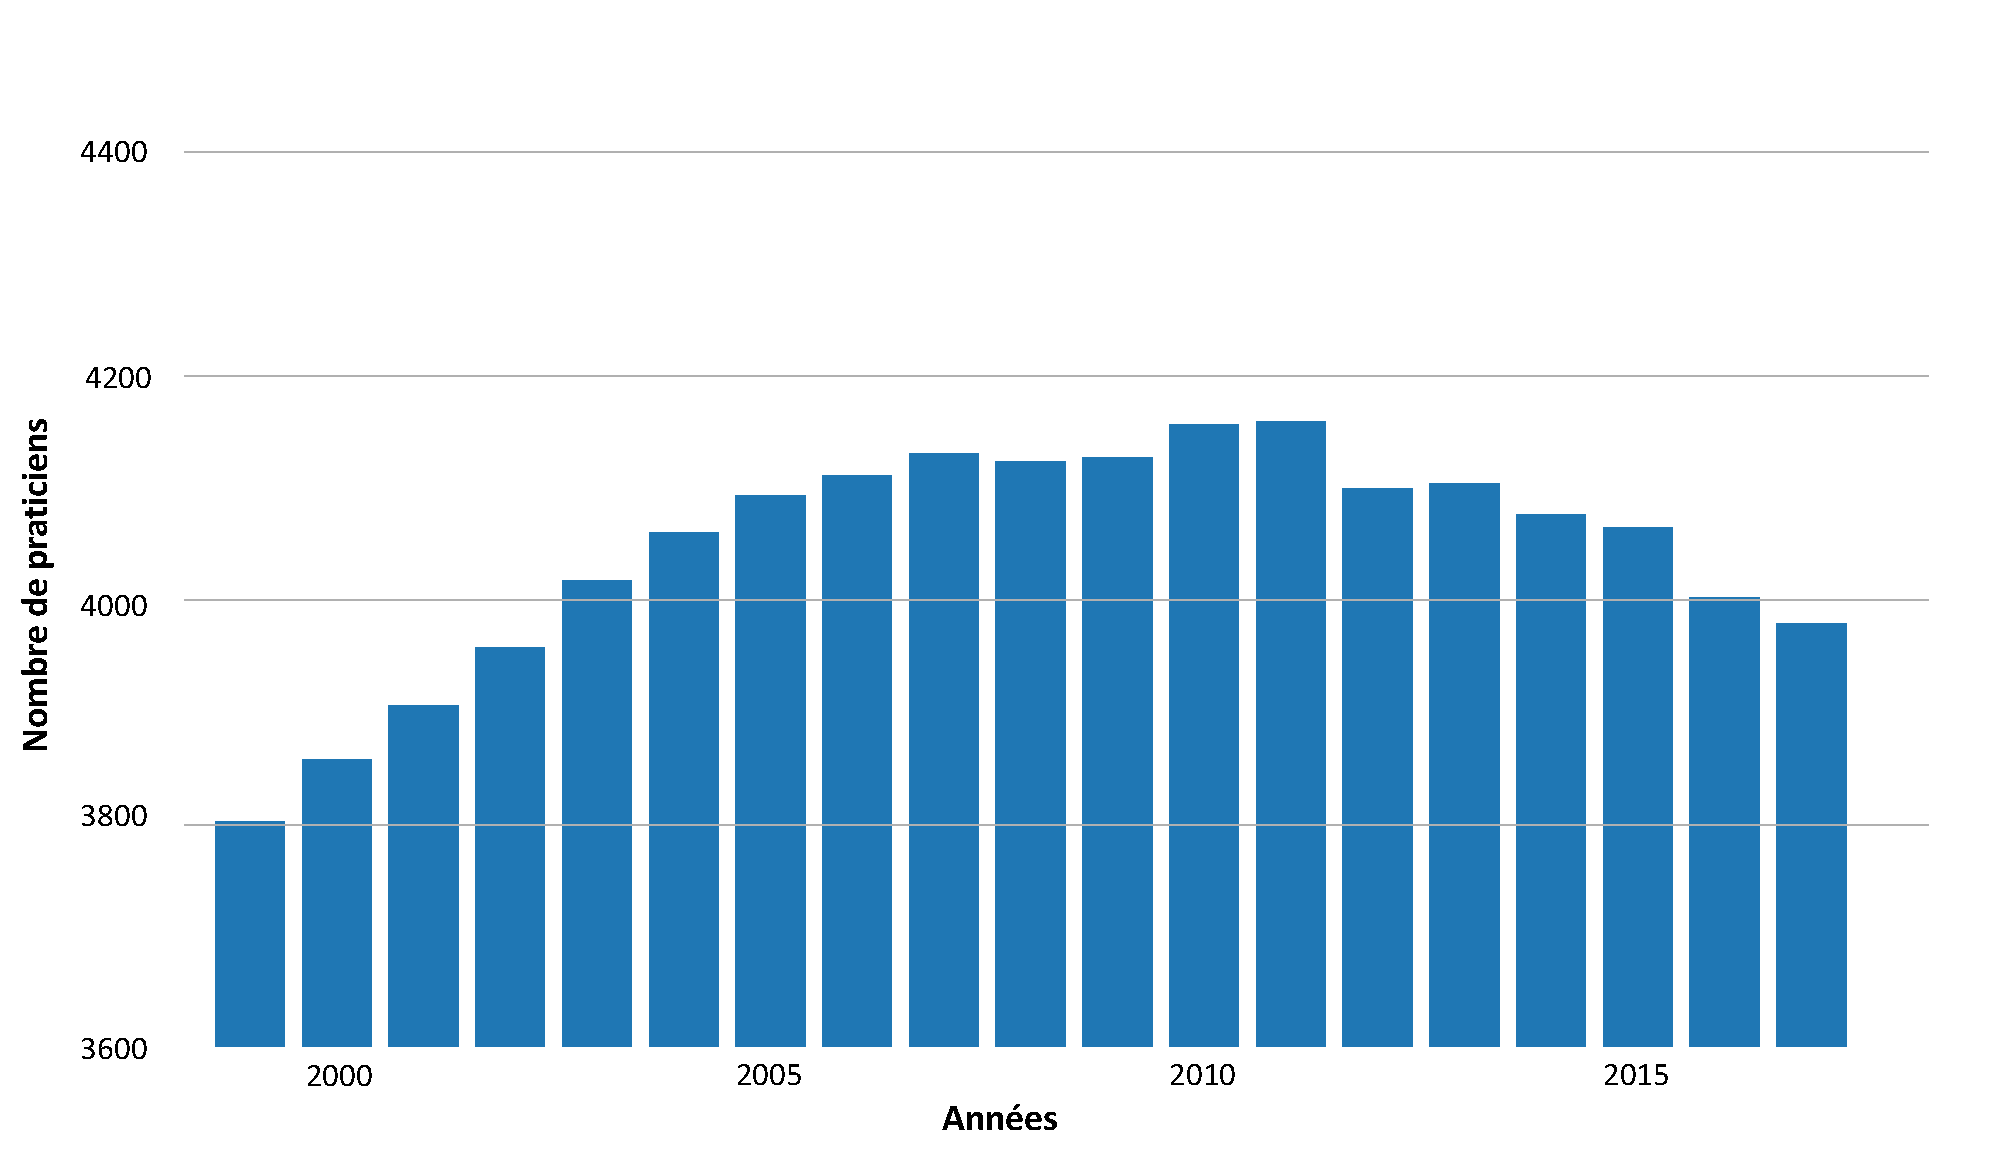
\includegraphics[width=\linewidth]{contents/i_introduction/resources/evolution_dermatologists.pdf}
    \caption{Évolution du nombre de dermatologues en France entre les années 1999 et 2017 \textsuperscript{\ref{footnote:number_dermatologists}}.}
    \label{fig:number_dermatologists}
\end{figure}\par
\addtocounter{footnote}{1}
\footnotetext[\thefootnote]{Source image~: Graphique généré à partir de données en provenance du site du  \href{http://www.data.drees.sante.gouv.fr/}{gouvernement} sur la santé. \label{footnote:number_dermatologists}}

Néanmoins, cette thématique ne demeure pas moins intéressante d’un point de vue scientifique. En effet, les 20 dernières années ont été portées par une forte tendance sur le sujet comme le démontre la \Cref{fig:evolution_publications}. Cette tendance est régie par plusieurs facteurs~:
\begin{itemize}
    \item Le besoin sociétal de la thématique, et l'intérêt porté par les industriels
    \item Le phénomène "machine learning", et ses récentes avancées (notamment avec l'apprentissage profond)
    \item Le "challenge" apporté par cette thématique, que nous développerons.
\end{itemize}\par

Ce travail tente d'apporter de nouveaux éléments de résolution, par l’apport notamment d’une dimension de multi modalité encore peu exploitée dans cette branche. 
\begin{figure}[H]
    \centering
    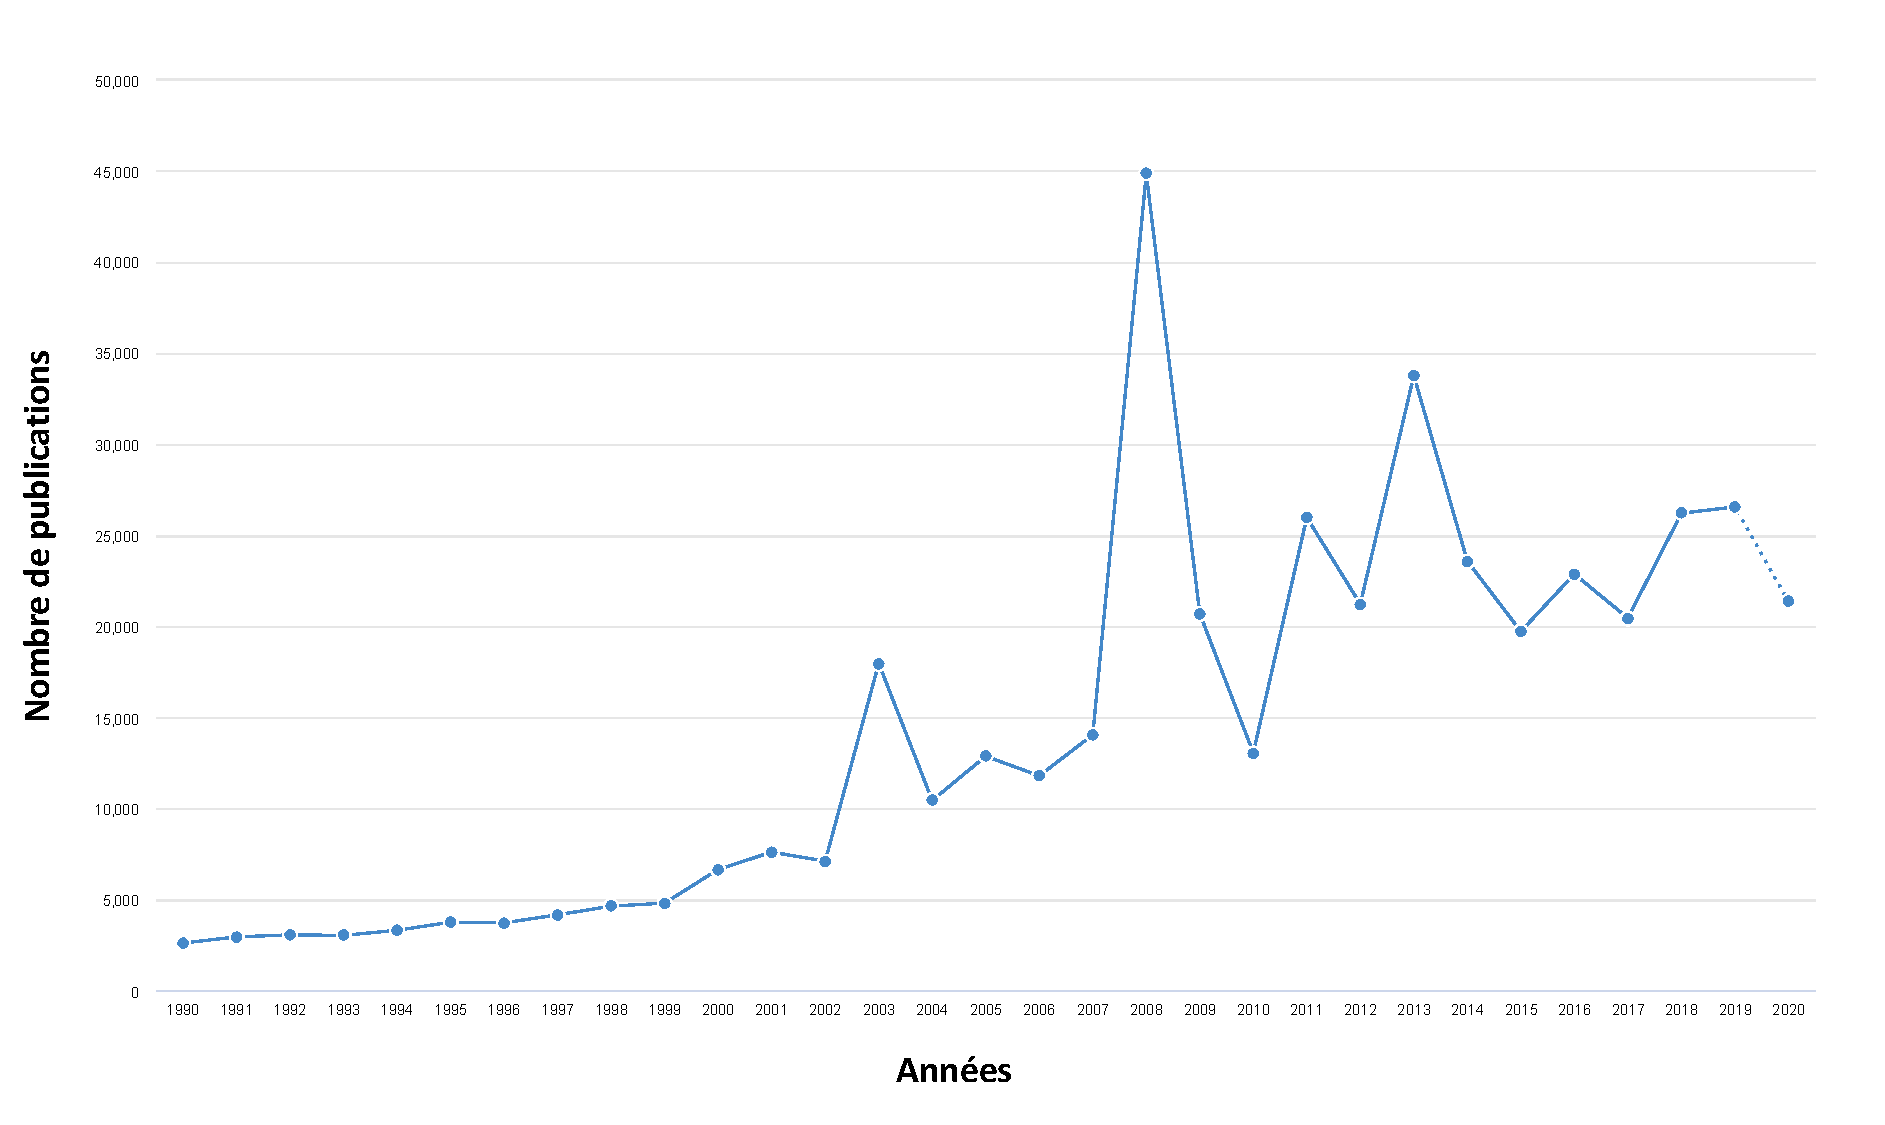
\includegraphics[width=\linewidth]{contents/i_introduction/resources/evolution_publications.pdf}
    \caption{Évolution de la recherche autour des termes "skin lesion computer diagnosis" durant ces 20 dernières années \textsuperscript{\ref{footnote:evolution_publications}}.}
    \label{fig:evolution_publications}
\end{figure}\par
\addtocounter{footnote}{1}
\footnotetext[\thefootnote]{Source image~: Graphique généré à partir de données en provenance du moteur de recherche \href{https://scholar.google.fr/}{Google Scholar.} \label{footnote:evolution_publications}}

Ce travail s'inscrit dans une démarche d'aide au diagnostic des lésions de la peau et particulièrement des pathologies de \gls{lm} et \gls{lmm}. De nombreux travaux se sont portés sur l'aide à la détection par ordinateur de lésions de la peau à partir d'une modalité unique d'imagerie. Néanmoins, peu d'entre eux s'intéressent à une démarche multimodale de cette thématique, soit par non-considération de cette application, soit par manque ou insuffisance de données à leur disposition.\par

La matière première mise à notre disposition permet une orientation de nos travaux dans le sens de la multimodalité. En effet, l'une des problématique majeure aujourd'hui en dermatologie est ce que les médecins qualifient de zone d'indécision, également appelée \textit{zone grise}. Il s'agit d'une catégorie de cas cliniques pour lesquels le médecin n'a pas à un instant $t$ suffisamment d'information ou de connaissances pour prendre une décision. Ces cas nécessitent souvent une prise en charge plus importante, avec l'aide d'autres spécialistes ou encore avec notamment de nouveaux examens plus spécifiques.\par

La finalité de ce travail est de proposer diverses techniques et outils permettant une aide à la décision dans la gestion de cette zone grise, et ainsi améliorer la prise en charge clinique en service de dermatologie. Ainsi, nous proposons un schéma macroscopique de cet objectif sur la \Cref{fig:scheme_reduce_indecision}.\par

\begin{figure}[H]
    \centering
    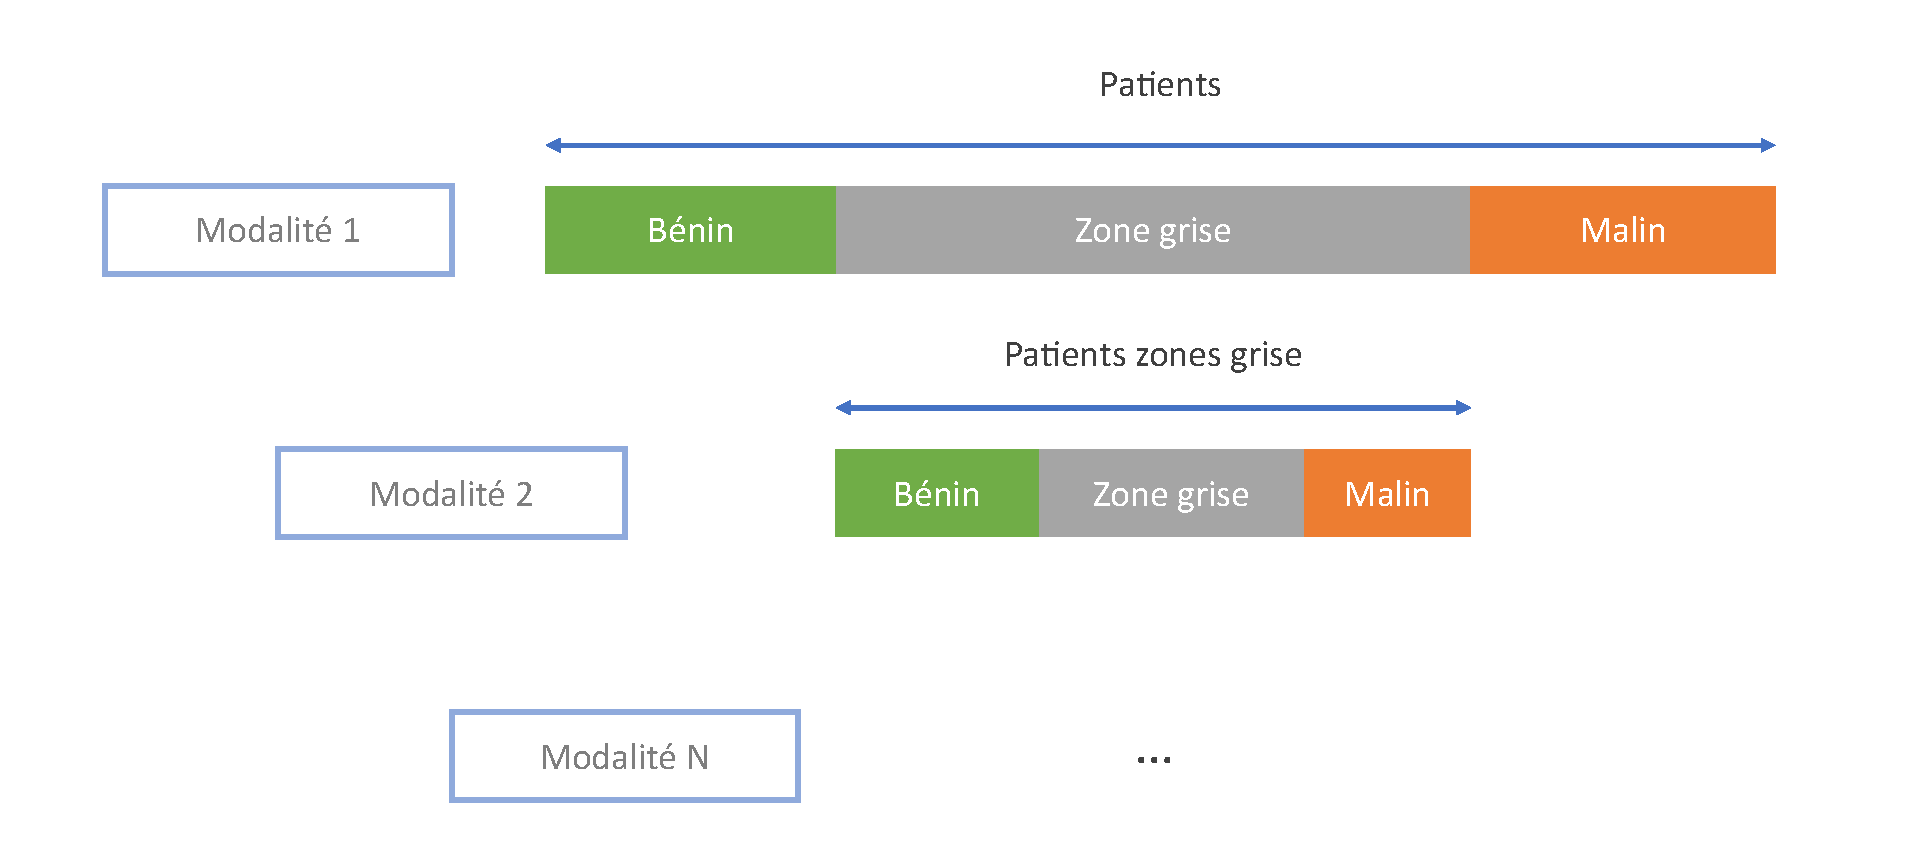
\includegraphics[width=\linewidth]{contents/i_introduction/resources/scheme_reduce_indecision.pdf}
    \caption{Représentation du processus de réduction de l'indécision du médecin ou \textit{zone grise}. L'objectif de ce travail consiste à réduire cette indécision des divers cas d'études en notre possession, par l'ajout de modalités d'imagerie en s'inspirant du processus cognitif des dermatologues.}
    \label{fig:scheme_reduce_indecision}
\end{figure}\par

Dans ce schéma idéal représenté sur la \Cref{fig:scheme_reduce_indecision}, les patients jugé avec une certaine certitude comme "bénin" ou "malin", seront exclus des procédures suivantes. Seuls les patients encore présents dans cette "zone grise" seront pris en charge pour des examens supplémentaires, par lesquels nous réitérons ce processus.\par 

A cette fin, nous mobiliserons des connaissances en provenance de divers champs d'applications propre~:
\begin{inlinerate}
    \item à la peau d'un point de vue médical, 
    \item aux modalités permettant l'observation des tissus,
    \item et à l'intelligence artificielle.
\end{inlinerate} Cette complémentarité est représentée sous forme de schéma macroscopique sur la \Cref{fig:scheme_our_work}.\par

\begin{figure}[H]
    \centering
    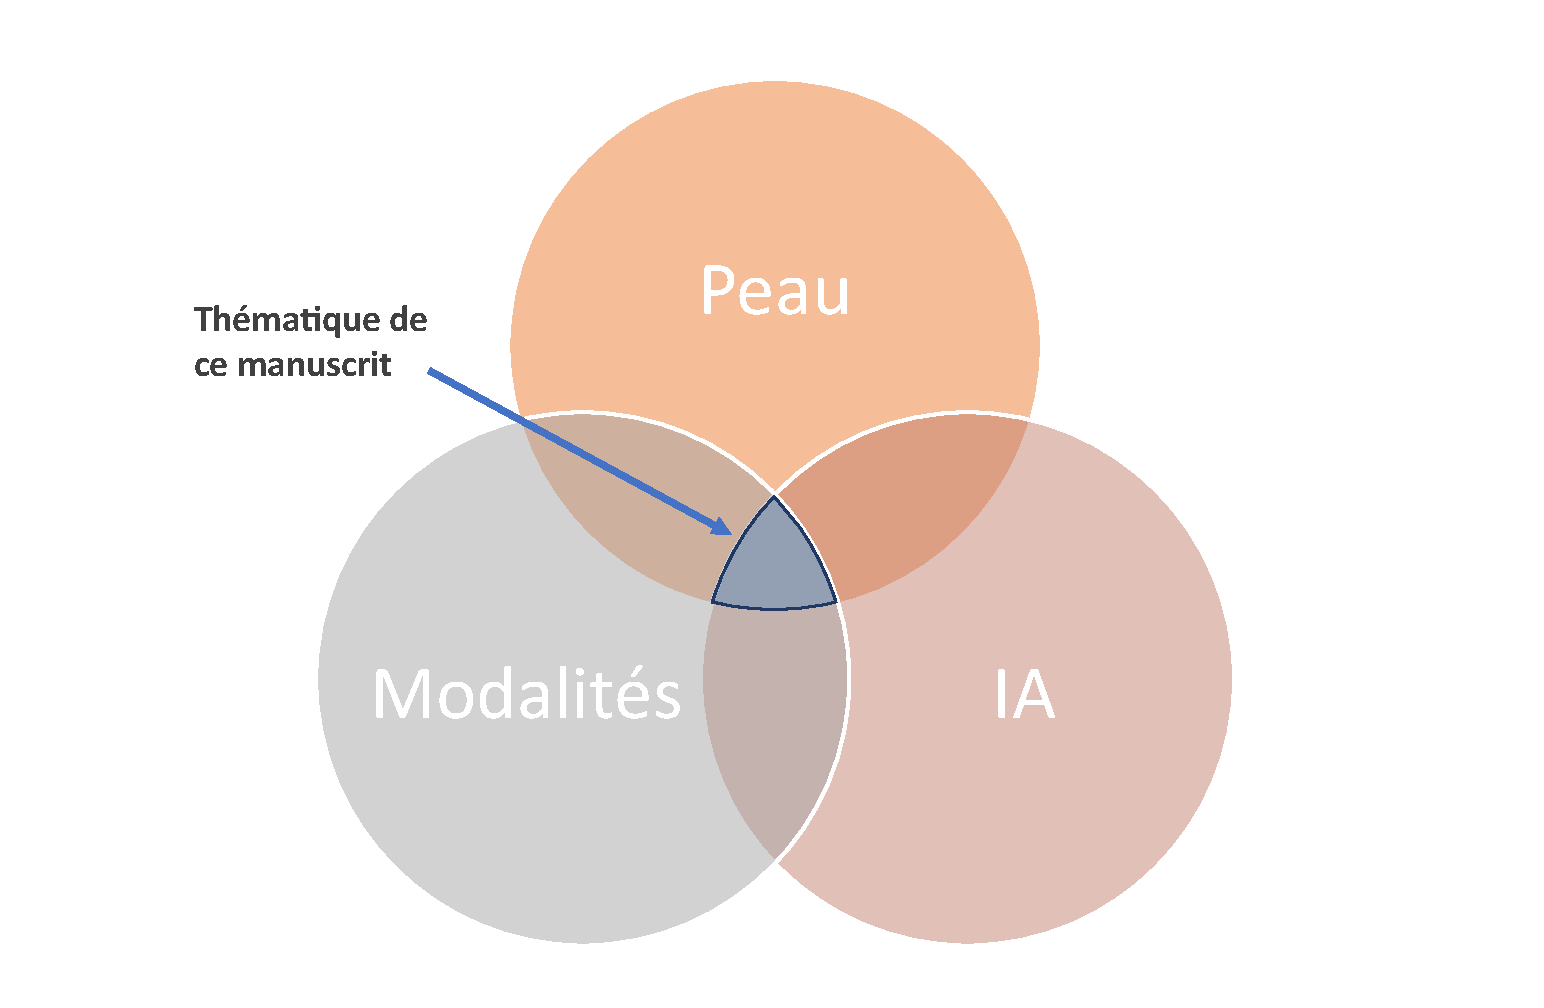
\includegraphics[width=0.8\linewidth]{contents/i_introduction/resources/scheme_our_work.pdf}
    \caption{Représentation macroscopique des domaines impliqués de cette thématique de recherche. Notre travail se retrouve ainsi aux confluents de connaissances de la peau, des modalités d'imagerie permettant son acquisition et des domaines de l'intelligence artificielle.}
    \label{fig:scheme_our_work}
\end{figure}\par

Dans un premier temps, nous aborderons le contexte de cette étude dans la \Cref{part:contexte}. Ainsi, nous débuterons au sein du \Cref{chap:chapter_1} par une présentation de la peau, l'organe majeur de cette étude. Puis, nous procéderons dans le \Cref{chap:chapter_2} à une mise en évidence des principes d'interaction entre la peau et la lumière, avant de présenter les techniques de visualisation mises à disposition des médecins. Pour finir cette partie, le \Cref{chap:chapter_3} met à la disposition du lecteur l'ensemble des connaissances d'intelligence artificielle sollicitées dans ce manuscrit.\par

Dans un second temps, nous nous consacrerons à l'aide de la \Cref{part:microscopy} au traitement de la modalité \gls{rcm}, qui met à notre disposition plusieurs images par lésions. A cet effet, nous débuterons par le traitement des images de cette modalité dans un \Cref{chap:chapter_4} dédié à la classification de ces images. Nous étendrons ces travaux dans le \Cref{chap:chapter_5}. Puis, nous terminerons l'analyse de cette modalité dans un \Cref{chap:chapter_6} dédié à la prise de décision au niveau d'une lésion.\par

Dans un dernier temps, nous nous consacrerons à la finalité de ce travail, celui de la multimodalité, par la \Cref{part:multimodal}. Le \Cref{chap:chapter_7} reprendra les travaux des autres modalités en notre possession ainsi que les conclusions de la \gls{rcm} et mettra en avant des méthodes d'agrégation de l'information.\par

% Part 1
\part{Contexte}
\label{part:contexte}
\renewcommand{\thechapter}{\arabic{chapter}}
\setcounter{chapter}{0}

\chapter{La peau et ses lésions}
\label{chap:chapter_1}
\chapterintro
Ce premier chapitre apporte une description de l'organe sujet de cette étude, à savoir la peau. Ainsi, ces quelques pages posent diverses bases en décrivant pas à pas des aspects qui permettent une compréhension de sa physiologie, de son fonctionnement et de ses rôles. De plus, ce chapitre est l'emplacement idéal pour aborder les multiples pathologies pouvant altérer cet organe.\par

Dans un premier temps, une explication de ses principales couches et composantes est réalisée par profondeur croissante. Dans un second temps, ce travail consacre une section dédiée à la présentation de quelques-unes de ses principales lésions. Par ailleurs, ces pages sont l'occasion d'aborder une première fois le Lentigo, pathologie centrale de cette étude, et tout particulièrement ses formes malignes~:~le \acrlong{lm} et le \acrlong{lmm}.\par
\newpage

\section{Présentation, composition et fonctions}
La première section de ce chapitre dédié à la peau propose d'introduire de manière synthétique la composition et le fonctionnement de cet organe, avant de présenter ses lésions. Ainsi, les différentes couches la définissant sont abordées par ordre croissant de profondeur lors des prochains paragraphes.\par

\subsection{Présentation}
Le terme \textit{peau} caractérise dans son sens le plus global, l’enveloppe externe propre aux vertébrés. Présente chez l’homme, elle est l’un de ses organes majeurs mais également l’un des plus lourds~:~chez un individu adulte d’un poids de \SI{70}{\kilo\gram}, elle représente une surface plane d’environ \SI{2}{\metre\squared}, soit une masse estimée à \SI{5}{\kilo\gram}~\cite{McGrath2010}. Son épaisseur diffère selon la zone du corps étudiée~:~de \SI{0,5}{\milli\metre} au niveau de zones fines telles que les paupières, à plusieurs centimètres sur les zones adipeuses. La surcharge pondérale influe également de manière importante sur son épaisseur, bien plus élevée chez des personnes souffrant d'obésité.\par

Bien que la peau soit l'un des premiers éléments visibles d'un individu, son fonctionnement et ses fonctionnalités sont souvent méconnus par la plupart des individus. Ses rôles sont pourtant multiples, parmi lesquels~:
\begin{itemize}
    \item un rôle \textbf{physique}, en apportant une protection contre le monde extérieur,
    \item un rôle \textbf{mécanique}, en limitant la perte d’eau ou en offrant une thermorégulation,
    \item un rôle \textbf{sensoriel}, en permettant l'appréhension de notre monde.
\end{itemize}\par

La dermatologie, branche médicale dédiée à l’étude de la peau, permet de mieux comprendre sa composition, son fonctionnement, ses vulnérabilités et permet d’apporter conseils, préventions et traitements dans le cas de certaines pathologies.\par

Cette barrière se décompose en diverses couches fondamentales~:~l’épiderme, la jonction dermo-épidermique, le derme et l’hypoderme, dont la représentation est visible sur la \Cref{fig:illustration_skin_kholoski}.\par
\begin{figure}[H]
    \centering
    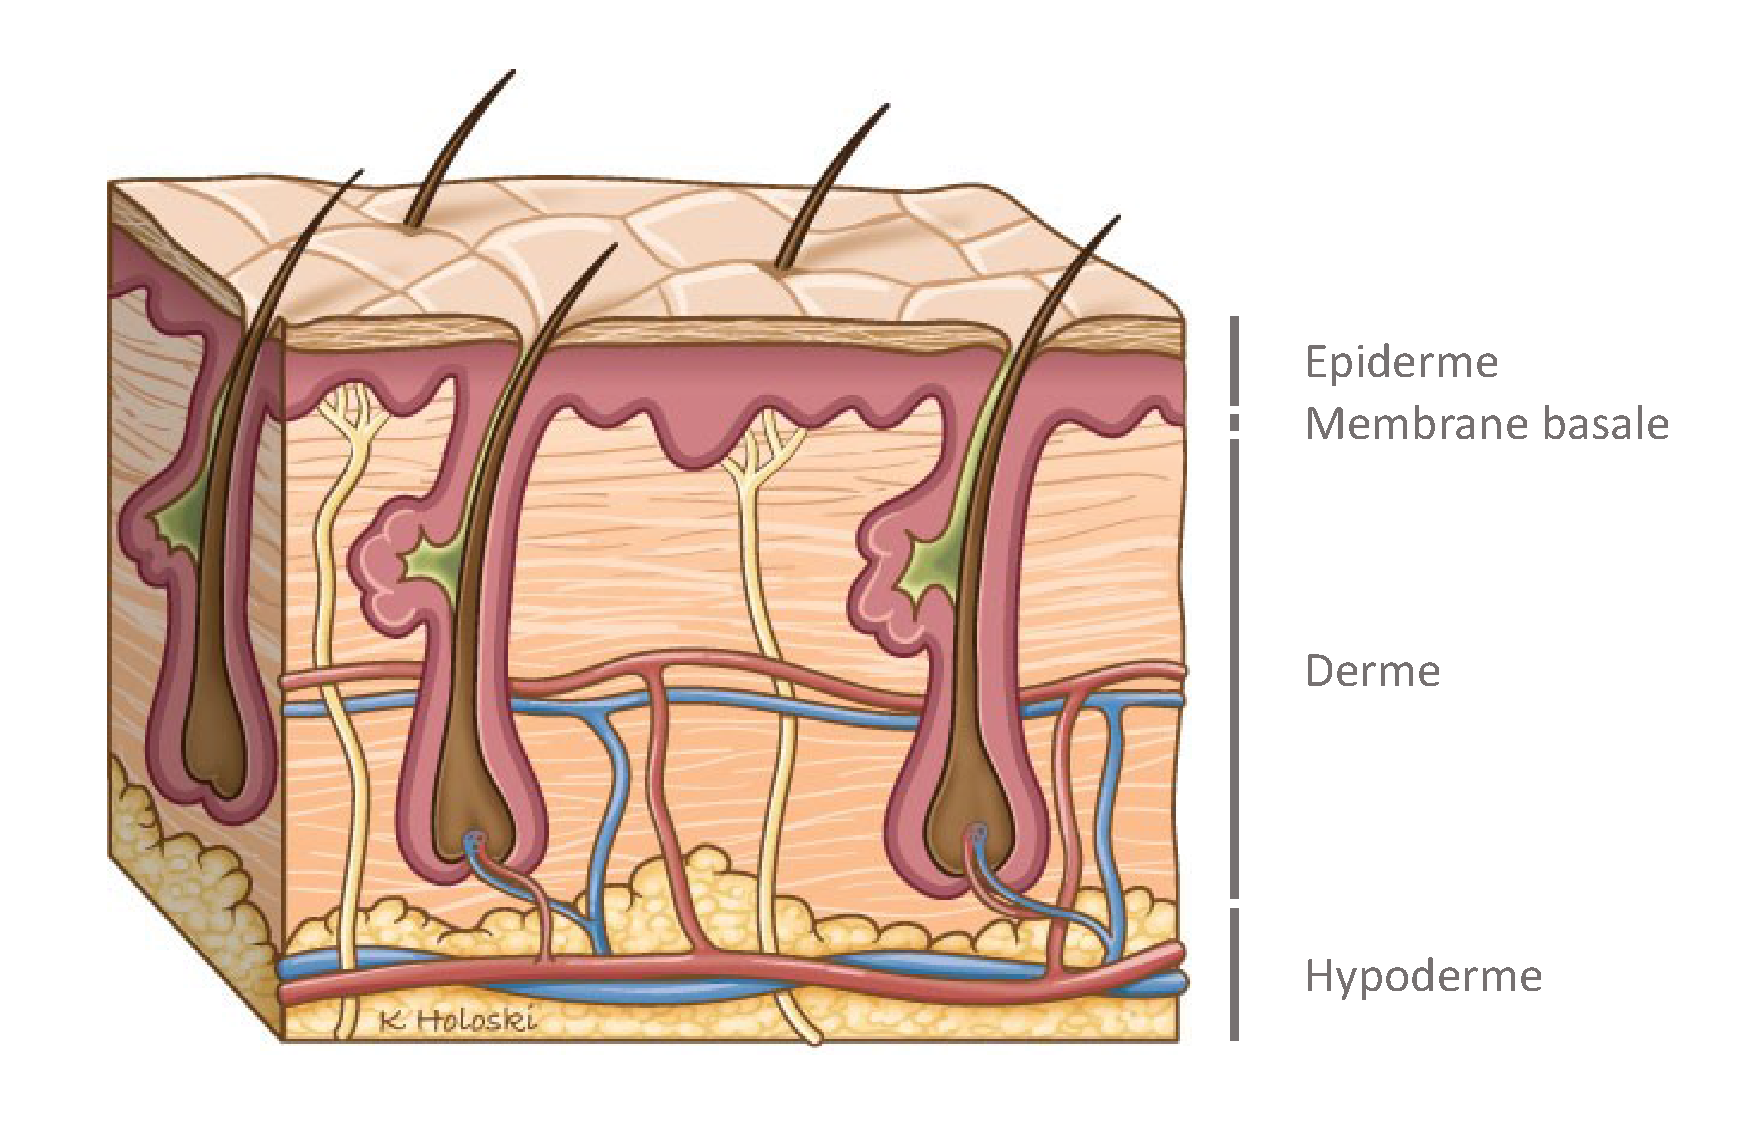
\includegraphics[width=0.6\linewidth]{contents/chapter_1/resources/illustration_skin_kholoski.pdf}
    \caption{Illustration de la peau et de ses diverses couches~\textsuperscript{\ref{footnote:illustration_skin_kholoski}}.}
    \label{fig:illustration_skin_kholoski}
\end{figure}\par 

\addtocounter{footnote}{1}
\footnotetext[\thefootnote]{Image source~:~Dessin par \href{http://kholoski.com/}{Kellie Holoski} – Illustrateur médical. \label{footnote:illustration_skin_kholoski}}

\subsection{Épiderme}
L’épiderme correspond à la couche superficielle de notre peau et mesure entre \SI{0,01}{\milli\metre} et \SI{0,1}{\milli\metre} d’épaisseur~\cite{Sandby-Moller2003}. Un aperçu des différents types de cellules composant cette couche est visible sur la \Cref{fig:illustration_epidermis_kholoski}, parmi lesquelles sont recensés~:
\begin{itemize}
    \item les \textbf{kératinocytes}~:~des cellules dont le rôle est d'offrir une protection contre l'environnement extérieur et d'apporter une imperméabilité. Elles représentent 90~\% des cellules de l'épiderme.
    \item les \textbf{cellules de Langerhans}~:~des cellules dont le rôle est immunitaire.
    \item les \textbf{cellules de Merkel}~:~des cellules dont le rôle est sensitif.
    \item les \textbf{mélanocytes}~:~des cellules dont le rôle est d'assurer la protection contre les rayonnements \gls{uv} par l'apport d'une pigmentation.
\end{itemize}\par

L'une des caractéristiques essentielles de cette couche est le fonctionnement de son processus de différenciation des cellules. Les kératinocytes migrent de la couche inférieure à la couche supérieure en subissant différentes modifications chimiques conduisant à la perte de leur noyau et à la mort de ces cellules. Ce processus porte le nom de kératinisation, et se subdivise en sous couches aux propriétés variées, respectivement par profondeur croissante~:~Cornée (\textit{Stratum corneum}), Transition (\textit{Stratum lucidum}), Granuleuse (\textit{Stratum granulosum}), Épineuse (\textit{Stratum spinosum}), Basale (\textit{Stratum basale}). Ces différentes couches peuvent être observées sur la \Cref{fig:illustration_epidermis_kholoski}. En fin de parcours, ces cellules perdent leur cohésion dans un processus de desquamation conduisant la peau à se renouveler.\par

 \begin{figure}[H]
    \centering
    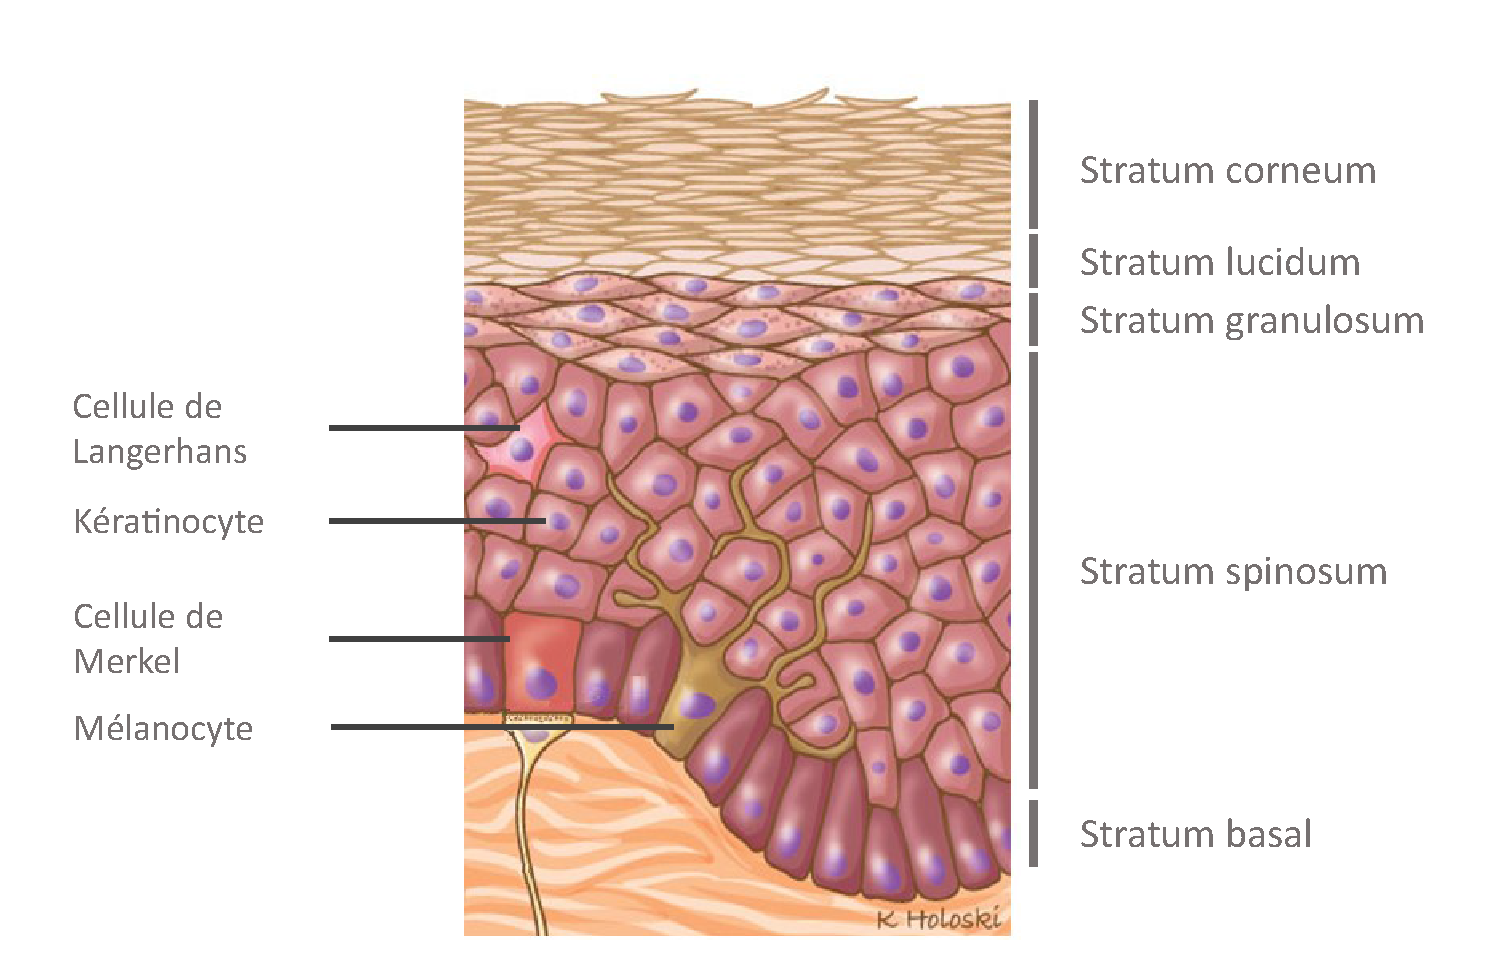
\includegraphics[width=0.9\linewidth]{contents/chapter_1/resources/illustration_epidermis_kholoski.pdf}
    \caption{Illustration des diverses couches de l'épiderme formées par un processus de différenciation ainsi que ses divers composés cellulaires \textsuperscript{\ref{footnote:illustration_epidermis_kholoski}}.}
    \label{fig:illustration_epidermis_kholoski}
\end{figure}\par

\addtocounter{footnote}{1}
\footnotetext[\thefootnote]{Image source~:~Dessin par \href{http://kholoski.com/}{Kellie Holoski} – Illustrateur médical. \label{footnote:illustration_epidermis_kholoski}}
\clearpage

\subsection{Jonction dermo-épidermique}
La \gls{jde}, également connue sous le terme de \textit{membrane basale}, se situe à la jonction de l’épiderme et du derme, assurant la cohésion entre ces deux couches. Selon la zone du corps considérée, son épaisseur varie de valeurs estimée entre \SI{60}{\nano\metre} et \SI{300}{\nano\metre}.\par

Représentée sur la \Cref{fig:illustration_basal_basement}, cette membrane est scindée en 2 parties~:
\begin{itemize}
    \item la \textbf{lame basale} (\textit{lamina basalis}), pouvant être subdivisée en deux nouvelles couches~:~la \textit{lamina lucida} et la \textit{lamina densa},
    \item la \textbf{lame réticulaire} ou zone fibrillaire (\textit{lamina reticularis}).
\end{itemize}\par

\begin{figure}[H]
    \centering
    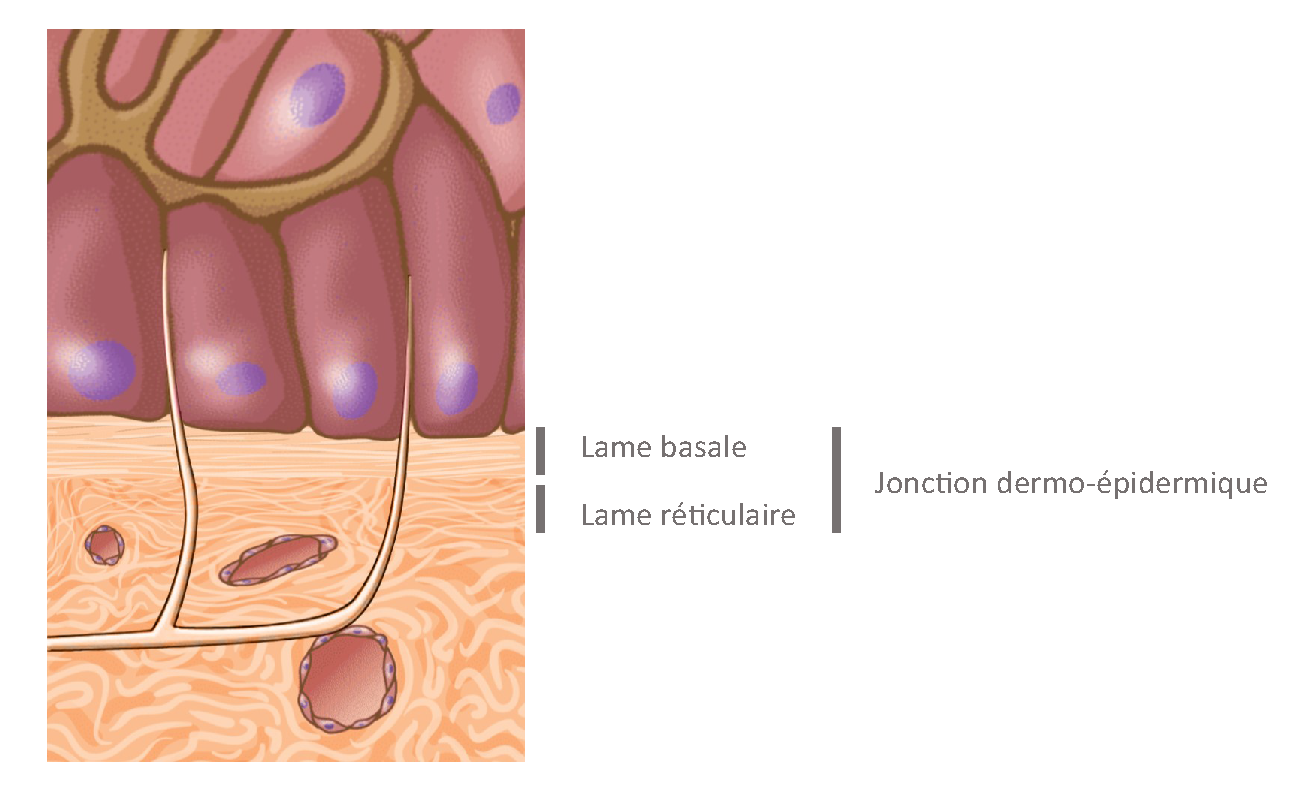
\includegraphics[width=\linewidth]{contents/chapter_1/resources/illustration_basal_basement.pdf}
    \caption{Illustration de la \acrlong{jde} \textsuperscript{\ref{footnote:illustration_basal_basement}}. Cette jonction dont le rôle est d'assurer une cohésion entre l'épiderme et le derme peut être subdivisée en deux sous couches~:~la lame basale et réticulaire.}
    \label{fig:illustration_basal_basement}
\end{figure}\par

\addtocounter{footnote}{1}
\footnotetext[\thefootnote]{Image source~:~Principles of Anatomy and Physiology – John Wiley \& Sons. \label{footnote:illustration_basal_basement}}

Il s’agit d’une zone fibreuse, composée de laminine mais également de collagène de type III / IV / VI lui conférant entre autres des propriétés de résistance mécanique et élastique. Ces fibres lui permettent d’assurer une cohésion entre épiderme et derme au travers de points d’ancrage. Sa seconde fonction essentielle est au travers d’un mécanisme de régulation des échanges moléculaires, permettant d’assurer la nutrition des cellules de base de l’épiderme. Pour finir, elle possède un rôle fondamental de ré-épidermisation essentiel à la cicatrisation.\par
\clearpage

\subsection{Derme}
Le derme est une couche d’une épaisseur estimée comprise entre \SI{0,5}{\milli\metre} et \SI{5}{\milli\metre}, composée majoritairement de collagène à hauteur de 80~\% (sur la matière sèche), et de fibres élastiques~\cite{McGrath2010}. Cette couche est traversée par de nombreux éléments dont~:~

\begin{itemize}
    \item des \textbf{vaisseaux sanguins} qui apportent des nutriments,
    \item des \textbf{vaisseaux lymphatiques} qui assurent une fonction immunitaire.
\end{itemize}\par

En outre, cette strate contribue de manière essentielle à des aspects de résistance et de contrainte mécanique de la peau, ainsi qu’aux mécanismes de thermorégulation et de cicatrisation de cette dernière. Enfin, cette couche tient un rôle essentiel dans la perception sensorielle (somesthésie) assurant d’une part des propriétés liées à la pression (mécanorécepteurs) mais également liées à la chaleur (thermorécepteurs). Outre ces fonctions, on lui attribue également un rôle nutritif important de par son irrigation sanguine.\par

La littérature scinde le derme en deux parties majeures, visibles en \Cref{fig:illustration_dermis_kholoski}, dont~:
\begin{itemize}
    \item le \textbf{derme Papillaire} (Papillary dermis), permettant essentiellement la thermorégulation,
    \item le \textbf{derme Réticulaire} (Reticular dermis), assurant la plupart des fonctions mécaniques.
\end{itemize}\par

\begin{figure}[H]
    \centering
    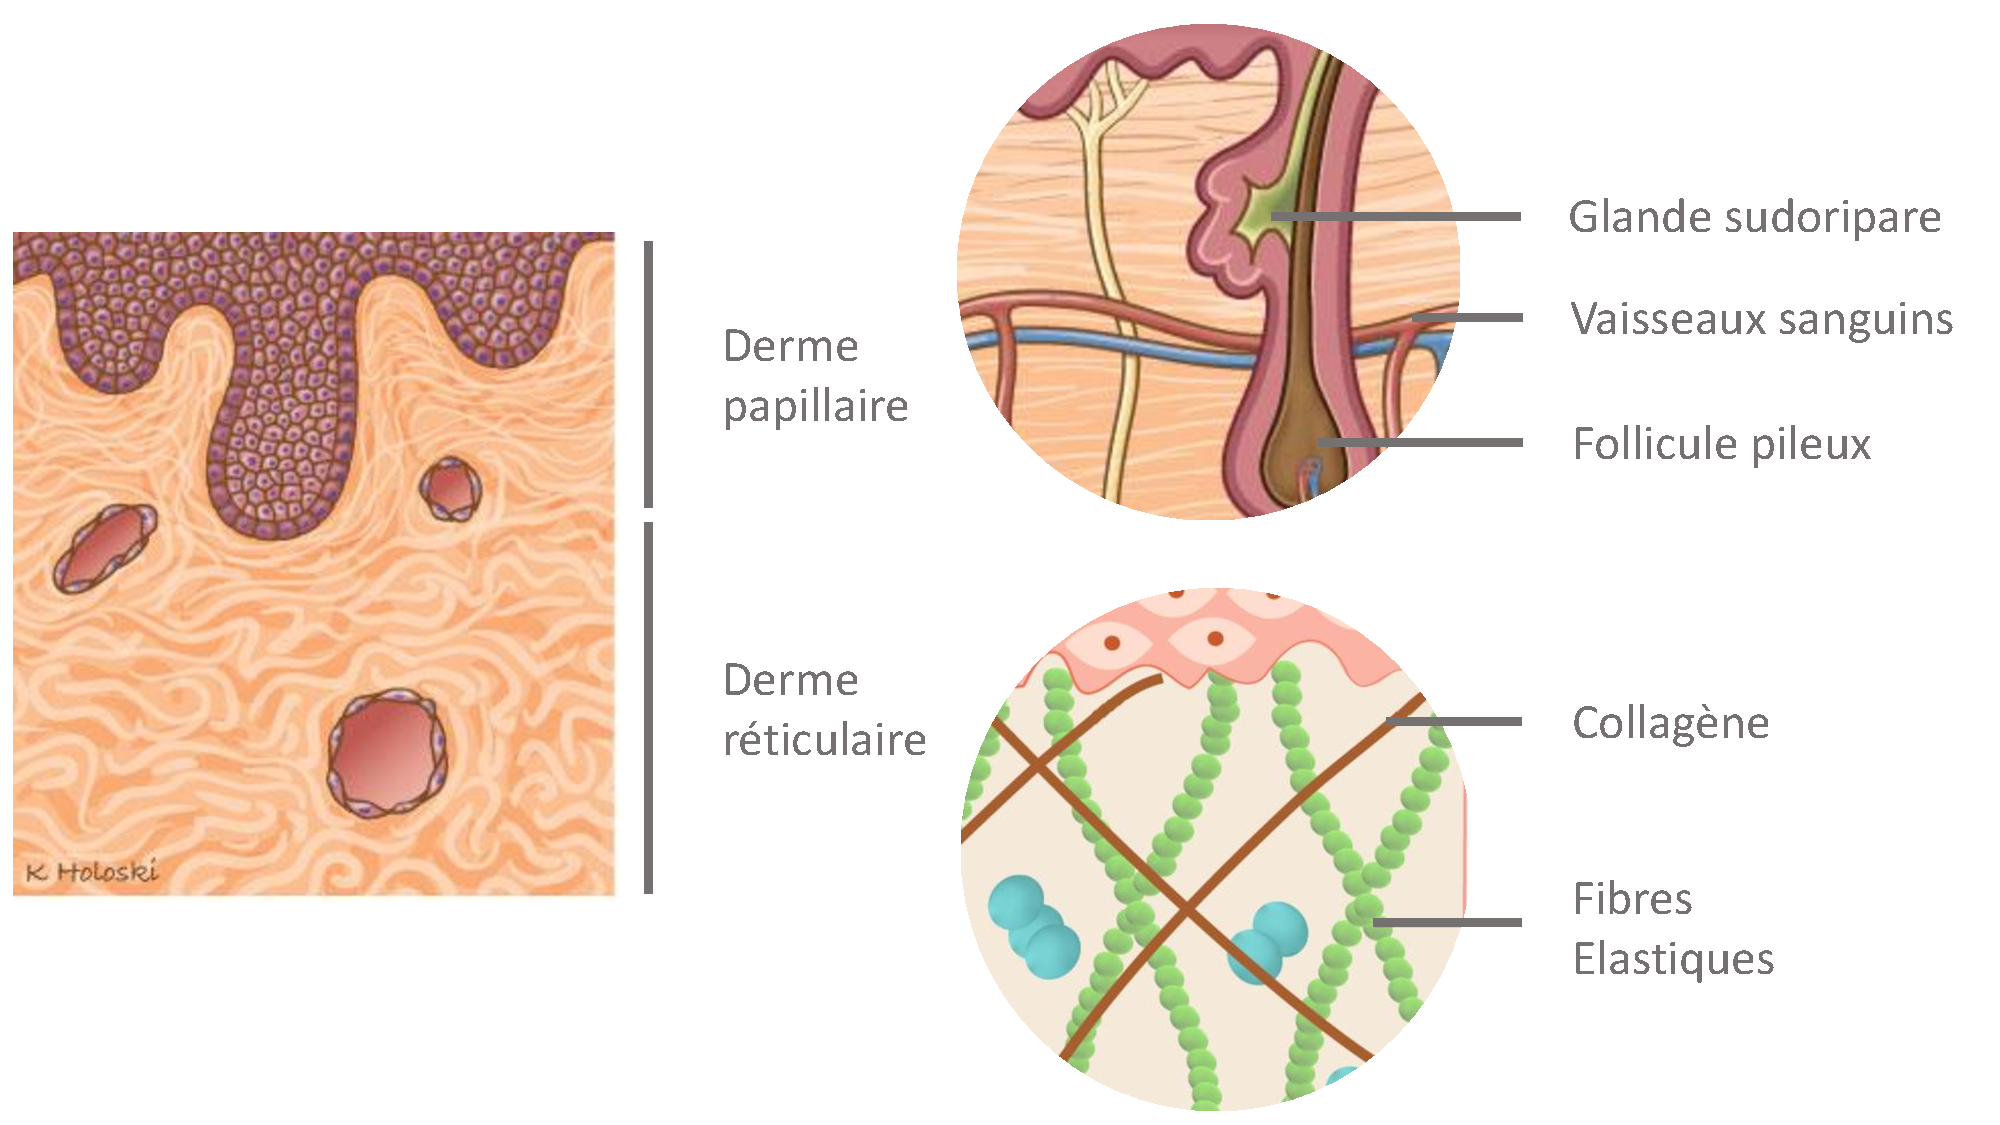
\includegraphics[width=\linewidth]{contents/chapter_1/resources/illustration_dermis_kholoski.pdf}
    \caption{Illustration de représentation du derme \textsuperscript{\ref{footnote:illustration_dermis_kholoski}}. Le derme est subdivisé en deux couches aux propriétés distinctes~:~le derme papillaire et réticulaire.}
    \label{fig:illustration_dermis_kholoski}
\end{figure}\par

\addtocounter{footnote}{1}
\footnotetext[\thefootnote]{Image source~:~Dessin par \href{http://kholoski.com/}{Kellie Holoski} – Illustrateur médical. \label{footnote:illustration_dermis_kholoski}}
\clearpage

\subsection{Hypoderme}
L’hypoderme, également appelé couche sous-cutanée, est un tissu présent sous le derme composé essentiellement de graisses (adipocytes, cellules spécialisées dans le stockage de graisses). Son épaisseur est extrêmement variable de \SI{0,1}{\centi\metre} à \SI[parse-numbers = false]{plusieurs}{\centi\metre}, selon~:
\begin{itemize}
    \item la zone considérée,
    \item l’âge du patient,
    \item l’alimentation,
    \item les prédispositions génétiques.
\end{itemize}\par

Cette couche de tissu assure diverses fonctions, dont~:
\begin{itemize}
    \item le passage des vaisseaux sanguins et lymphatiques, ainsi que celui des nerfs jusqu’au derme
    \item l’interface entre les structures sous cutanées et la peau.
\end{itemize}\par

\subsection{Types de peau}
Il est nécessaire afin de bien aborder ce sujet et ses problématiques, d’être conscient des variations inter individus. Pour répondre partiellement à ces variations, Fitzpatrick a établi une classification des profils type de peau, visant à caractériser leur réaction suite à l’exposition au soleil. Ce travail a également permis de créer une association entre les profils type et les risques de cancers associés~\cite{Fitzpatrick1988}.\par

Cet aspect est un élément important à prendre en compte lors de notre appréhension de la problématique. En effet, la plupart des travaux d'aide au diagnostic par ordinateur de la littérature ne décrivent pas les types de peau employés~\cite{Celebi2007,Wiltgen2008,Koller2011}. Néanmoins, les échantillons mis en avant par ces travaux semblent majoritairement axés sur les types I et II selon l'échelle de Fitzpatrick. Certaines pathologies sont ainsi plus propices à se développer sur un type de peau en particulier~\cite{Narayanan2010}. De plus, une même pathologie peut diverger en termes de caractéristiques~\cite{Tuma2015}. La \Cref{fig:scheme_fitzpatrick_scale} propose une synthèse visuelle des types de peau identifiés par Fitzpatrick, mais également de la résistance aux \gls{uv} et du risque de cancer associé à chacun d'entre eux.\par

\begin{figure}[H]
    \centering
    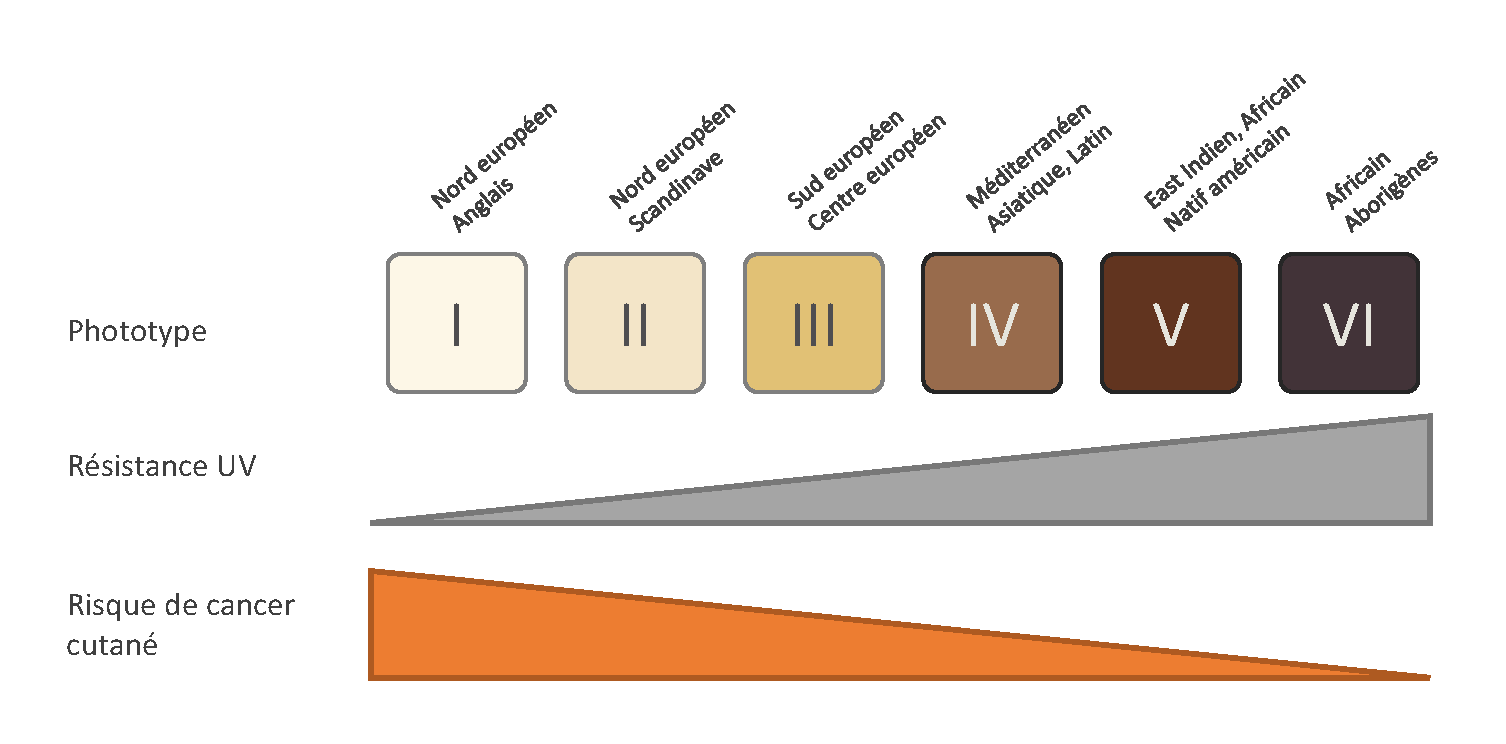
\includegraphics[width=0.8\linewidth]{contents/chapter_1/resources/scheme_fitzpatrick_scale.pdf}
    \caption{Échelle de Fitzpatrick associant type de peau et propriétés associées~\cite{Fitzpatrick1988}.}
    \label{fig:scheme_fitzpatrick_scale}
\end{figure}


\section{Lésions de la peau}
Notre sujet abordant les lésions de la peau, il convient de définir le terme lésion pour bien situer l’objet de notre recherche. Selon PubMed, une lésion « correspond à toute anomalie touchant les tissus d’un organisme, généralement provoquée par une maladie ou par un traumatisme. » \textsuperscript{\ref{footnote:lesion_pubmed}}.\par
\addtocounter{footnote}{1}
\footnotetext[\thefootnote]{Source~:~Définition par \href{https://www.ncbi.nlm.nih.gov/pubmedhealth}{PubMed Health}. \label{footnote:lesion_pubmed}}

Les lésions de la peau correspondent à un terme générique caractérisant une partie de la peau ayant, en comparaison de la peau l’entourant, une croissance/apparence ou structure qui diffère de tissus considérés comme sains. Ces lésions peuvent ainsi être pré-natales ou post-natales, comporter diverses formes et peuvent présenter différents risques.\par

Ces lésions sont une catégorie très vaste dont les origines sont multiples, et peuvent être spécifiées par des termes complémentaires. Ainsi, le terme de \textit{lésion pigmentaire} caractérise les lésions affectant la peau par la présence de pigmentations essentiellement liées à la mélanine ou aux globules rouges.\par

Ces lésions sont sommairement présentées au travers de ces quelques pages. D'une part, les \textbf{lésions bénignes} sont abordées à l'aide d'une brève sous-section, et d'autre part, les \textbf{lésions malignes} sont traitées plus en détail lors d'une seconde sous-section présentant les pathologies majeures mais également les cas de \acrlong{lm} et \acrlong{lmm}.\par

\subsection{Lésions bénignes}
Ces lésions désignent les diverses altérations classées comme sans conséquences graves pour la santé d'un individu, néanmoins ces lésions peuvent présenter un terrain pour des lésions plus dangereuses.\par

L'une des lésions bénignes les plus communes est le \textbf{naevus mélanocytaire}, à l’apparence de structures souvent circulaires ou ovales présentes en surface de peau chez l’homme. Les naevus sont susceptibles d’évoluer au cours du temps et peuvent rarement aboutir à un mélanome. La plupart d'entre eux apparaissent durant les trente premières années de vie en moyenne et présentent des couleurs variées, avec des teintes allant d'un rose rougeâtre jusqu'au noir. Parmi ces lésions, peuvent être cités~:
\begin{itemize}
    \item le \textbf{nævus commun}, également connu sous le nom de \textit{grain de beauté}, est l'une des lésions les plus fréquentes composée de mélanocytes regroupés en amas.
    \item le \textbf{nævus atypique} se caractérise souvent par une pigmentation variable et des bordures irrégulières.
    \item le \textbf{nævus congénital} apparaît en début de vie, le plus souvent sous forme de tâche.
    \item le \textbf{nævus de Spitz} s’apparente souvent à un mélanome de par sa croissance rapide (souvent de 2 à 6 mois) ainsi qu’une couleur brun-rouge.
    \item le \textbf{phénomène de Sutton} caractérisé par une dé-pigmentation aux abords d’un naevus existant sur une durée de quelques semaines à quelques mois.
\end{itemize}\par

La meilleure des solutions est de réaliser une surveillance régulière chez les individus afin de s'assurer que ces lésions ne dégénèrent pas en pathologies malignes.\par

\subsection{Lésions malignes}
Le terme malin qualifie dans le contexte de ce manuscrit une pathologie cancéreuse dont les conséquences peuvent aller jusqu'au décès de l'individu sans l'intervention adéquate d'un spécialiste. Ces cancers de la peau sont issus d’une division ou d’une mutation anormale de cellules de la peau et le risque de décès est principalement causé par des métastases de la tumeur initiale. Certaines de ces tumeurs peuvent être difficiles à prendre charge car susceptibles de réapparaître sans prendre une marge de sécurité suffisante lors de l'excision. Outre le décès, ces lésions peuvent donc à des stades avancés et selon le type de tumeur engendrer des lésions cicatricielles permanentes à la suite de leur prise en charge chirurgicale, mais également des gênes corporelles importantes. Il est donc crucial de détecter au plus tôt ces lésions et de procéder à leur prise en charge le plus rapidement possible afin de limiter les conséquences voir les désagréments.\par

Ces cancers résultent pour la plupart d’une exposition aux \gls{uv}, principal facteur de mutation. D’autres facteurs tels que le tabagisme, les virus, des prédispositions génétiques ou encore l’utilisation de médicaments immunosuppresseurs peuvent favoriser leur apparition. Les prochaines sous-sections reprennent pathologies malignes de la peau les plus importantes par ordre d'incidence.\par

\subsubsection{Carcinome spinocellulaire (ou épidermoïde)}
Les \gls{csc} se développent à partir de l'épiderme dont la croissance devient incontrôlée. Cette pathologie peut prendre de multiples apparences, variant de simples plaques rouges à des cas de plaies ouvertes. Cette pathologie est à même de provoquer des métastases chez un individu, et donc de se propager.\par

Ce type de cancer est au second rang des cancers cutanés les plus graves, principalement lié à cette caractéristique de propagation. Ces cancers émergent le plus souvent de zones exposées régulièrement au soleil telles que le visage, les oreilles, le cou, \ldots. Ces zones dénotent le plus souvent des symptômes liés au dommage du soleil, tels que~:
\begin{itemize}
    \item des rides,
    \item des tâches,
    \item une perte d’élasticité.
\end{itemize}
Les prédispositions génétiques, les conditions de travail et le sexe d’un individu sont autant de facteurs pouvant influer sur l’apparition de ce type de cancer.\par

\subsubsection{Carcinome basocellulaire}	
Le \gls{cbc} correspond à une tumeur maligne développé à partir des cellules basales. Il s’agit de la forme de cancer de la peau la plus fréquente chez l'humain. Ses conséquences médicales sont le plus souvent d'ordre cicatriciel, liées à l'exérèse de cette tumeur. Néanmoins, le coût sociétal engendré est considérable du fait de leur grande fréquence. En effet, ces cancers ont peu de risques de métastases et sont donc moins enclins à se propager à l’ensemble de l’organisme et de provoquer la mort du patient. Ce cancer peut résulter de divers facteurs comme ses homologues, dont les principaux restent la surexposition au soleil ou la défaillance du système immunitaire.\par

\subsubsection{Mélanome}
Le mélanome est l'un des cancers de la peau les plus agressifs, également qualifié de tumeur mélanocytaire car se développant à partir de mélanocytes. Ce type de cancer apparaît dans environ 70~\% des cas sur une peau saine et dans les 30~\% restant sur un naevus présent au préalable. Bien que cette tumeur ne représente que 2~\% des cas de cancers de la peau~\cite{Tortora2012}, il s’agit en contrepartie du type le plus agressif de cancer de la peau. Au niveau mondial et pour l'année 2015, ce cancer a été détecté chez plus de 350 000 personnes et a provoqué le décès de 59 800 individus~\cite{Karimkhani2017}. Son incidence est fortement aggravée par l’exposition prolongée au soleil et plus particulièrement aux \gls{uv}. Par ailleurs, les types I et II sur l’échelle de Fitzpatrick sont les types de peau les plus concernés par cette pathologie.\par

Deux types de catégories de mélanomes sont recensés avec d’une part les pathologies superficielles caractérisant les mélanomes qui présentent une phase d’extension épidermique (extension horizontale) et d'autre part les pathologies qui présentent une phase de développement en profondeur (extension verticale).\par

La première catégorie, dont la sévérité est évaluée par l'épaisseur (indice de Breslow) et l'extension en profondeur (indice de Clark~\cite{Clark1969} - \Cref{fig:illustration_clarklevels_kholoski}), distingue trois types de pathologies~:
\begin{itemize}
    \item les mélanomes d'extension superficielle – environ 70~\% des mélanomes,
    \item les mélanomes acro-lentigineux – environ 10~\% des mélanomes,
    \item les \textbf{\acrlong{lm}} et de \textbf{\acrlong{lmm}} – environ 10~\% des mélanomes~\cite{LeGal2011}.
\end{itemize}

La seconde catégorie est composée des mélanomes nodulaires, dont l'évolution plus rapide est liée à un développent vertical dès les premiers symptômes. L'indice de Clark est également employé dans le but de caractériser les stades de ce type de mélanomes~\cite{Clark1969}, représenté sur la \Cref{fig:illustration_clarklevels_kholoski}.\par

\begin{figure}[H]
    \centering
    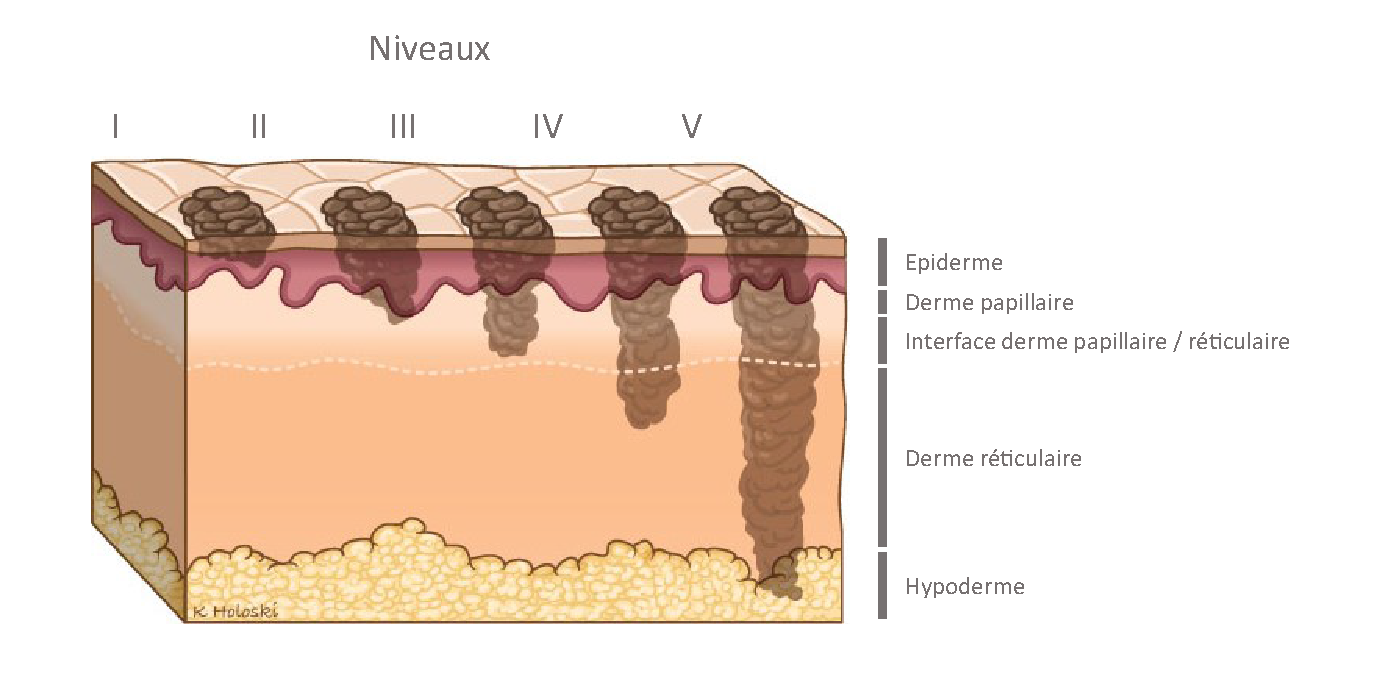
\includegraphics[width=0.9\linewidth]{contents/chapter_1/resources/illustration_clarklevels_kholoski.pdf}
    \caption{Illustration de l'indice de Clark~\cite{Clark1969}, défini par plusieurs niveaux de progression \textsuperscript{\ref{footnote:illustration_clarklevels_kholoski}}.}
    \label{fig:illustration_clarklevels_kholoski}
\end{figure}\par

\addtocounter{footnote}{1}
\footnotetext[\thefootnote]{Image source~:~Dessin par \href{http://kholoski.com/}{Kellie Holoski} – Illustrateur médical. \label{footnote:illustration_clarklevels_kholoski}}

\subsubsection{Une pathologie particulière~:~le Lentigo maligna}
\label{subsec:lentigo}
Les termes de \acrfull{lm} et de \acrfull{lmm} correspondent à des tumeurs qui touchent les zones les plus exposées chez un individu tel que le visage chez les populations de plus de 60 ans. Comme précédemment énoncé, ils représentent environ 10~\% des cas de mélanomes mais tendent à augmenter ces dernières années et vont désormais jusqu'à toucher les populations considérées comme jeunes. Le facteur explicatif le plus probable à ce jour est l'exposition au soleil croissante chez les différentes populations~\cite{Baccard2009, LeGal2011, LeDuff2014}.\par

Le \gls{lm} résulte d'une prolifération de cellules malignes mélanocytaire au sein de la couche basale de l'épiderme. Son développement progressif est constitué de plusieurs étapes successives, dont~:
\begin{inlinerate}[label=(\alph*)]
    \item l'apparition de points gris et de globules,
    \item l'apparition d'ouvertures asymétriques et de demi-cercles,
    \item l'apparition de structures rhomboïdales et de cercles,
    \item l'apparition de cercles imbriqués,
    \item l'apparition de follicules comblés,
    \item et pour finir l'apparition de zones sans structures visibles.
\end{inlinerate} 
Les étapes propres à ce développement sont schématisées sur la \Cref{fig:illustration_surface_progression}. Ces observations typiques du développement de cette lésion vont dans le sens d'un suivi régulier par un expert permettant de lever toute ambiguïté.\par

En outre, le \textbf{\gls{lm}} est considéré comme un \textit{stade 0} également considéré sous le terme de \textit{melanoma-in-situ}. Lorsque cette prolifération se propage aux cellules profondes de la peau au-delà de la \gls{jde} par le biais des follicules pileux, cette pathologie est alors qualifiée de \textbf{\gls{lmm}} et donne lieu à un risque important de métastases résultant de cette infiltration de cellules cancéreuses. Bien que la transition de \gls{lm} à \gls{lmm} soit souvent d'une dizaine d'années, il n'est pas isolé d'observer des cas cliniques dont l'évolution a lieu entre deux examens bi-annuels~\cite{Mckenna2006, LeGal2011}. 

\begin{figure}[H]
    \centering
    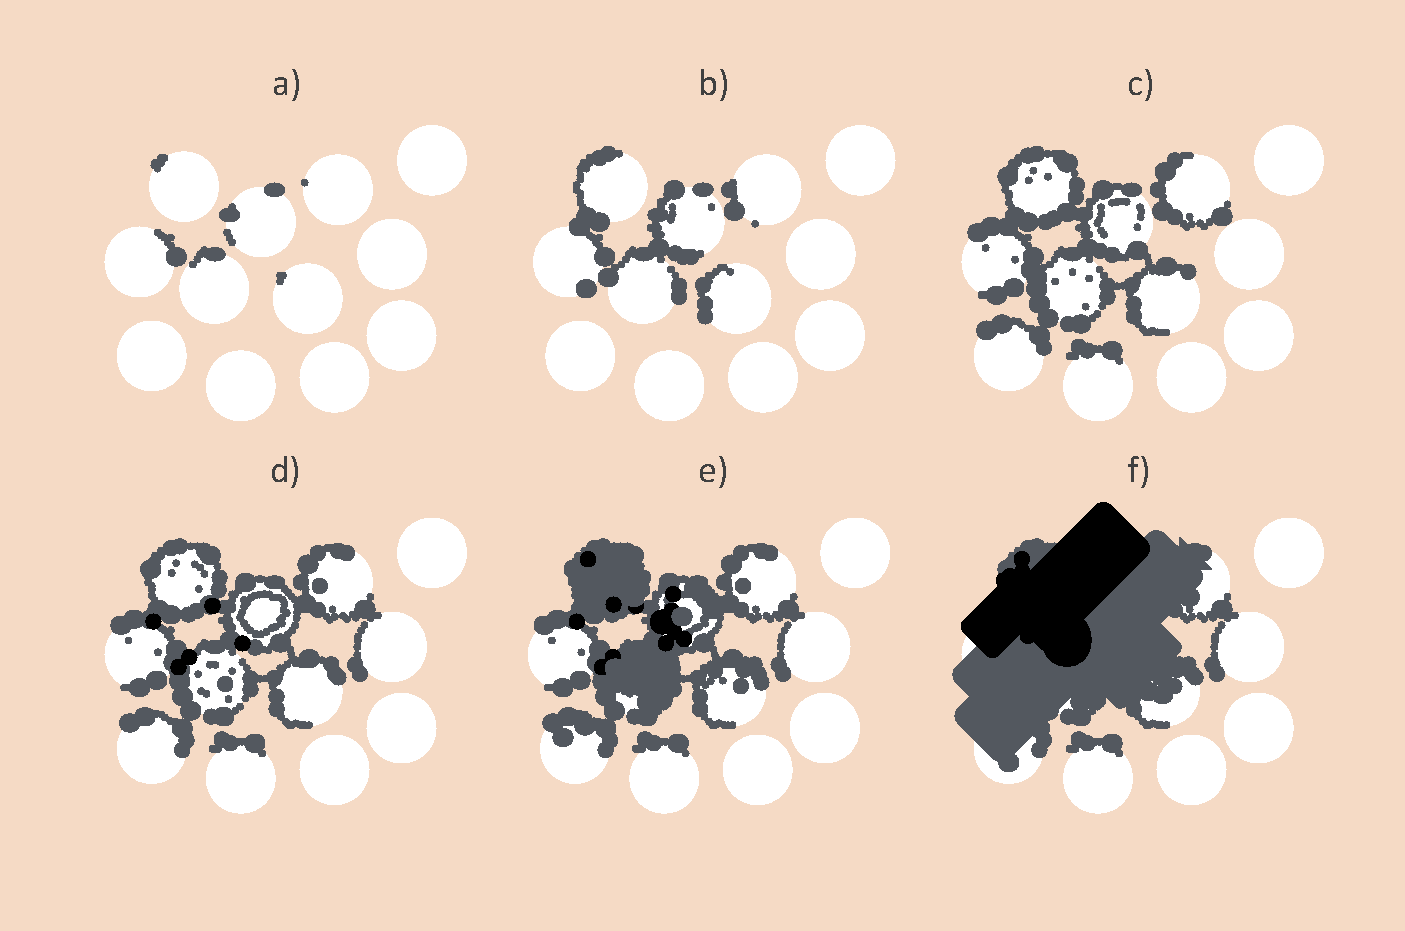
\includegraphics[width=\linewidth]{contents/chapter_1/resources/illustration_surface_progression.pdf}
    \caption{Illustration par Jean-Luc Perrot des stades d'évolution d'un \gls{lm}. Les points blancs permettent de représenter les follicules pileux.}
    \label{fig:illustration_surface_progression}
\end{figure}\par

Les pathologies de \gls{lm} sont difficiles à diagnostiquer à l’œil nu et peuvent être confondues avec des pathologies bénignes telles qu'un \gls{ls}, une \gls{ks} ou une \gls{kap}~\cite{LeDuff2014}. Par ailleurs, les \gls{lm} sont très différents des autres types de mélanomes dont les limites peuvent être difficiles à définir. En effet, leur prolifération périphérique peut-être discrète voire non pigmentée~\cite{LeGal2011}. En termes de signes propres, le \gls{lm} se caractérise le plus souvent par une macule pigmentée, et par la présence de bordures et de pigmentations irrégulières dont la taille atteint aisément une dizaine de centimètres. Pour sa part, le \gls{lmm} se présente sous la forme d'une lésion tumorale papuleuse ou nodulaire~\cite{Mckenna2006, LeGal2011}.\par

Afin de lever cette ambiguïté, il est possible d'avoir recours à \textbf{l'histopathologie}. Le dermatologue procède à l'excision par biopsie d'un tissu intra-lésionnel considéré comme pathologique, puis ce même tissu est préparé afin d'être observé par microscope. D'une part, cette procédure est relativement longue à réaliser et d'autre part représente une charge financière importante une fois rapportée au coût par examen. En addition, il s'agit d'une procédure incommodante pour le patient, pouvant échouer si le prélèvement est effectué en dehors d'un foyer mélanocytaire~\cite{LeGal2011}. Des exemples histologiques de pathologie de \gls{lm} peuvent être observés sur la \Cref{fig:example_lentigo_maligna} - en d) et e).\par

Cette difficulté à distinguer ces pathologies et les limitations induites par l'histopathologie conduisent à l'utilisation de dispositifs d'imagerie \textit{in-vivo} prévus pour ce domaine d'application. Ainsi, parmi les plus utilisés dans ce domaine peuvent être cités~:
\begin{inlinerate}
    \item la dermatoscopie,
    \item et la microscopie confocale par réflectance.
\end{inlinerate} Des exemples d'images de pathologies de \gls{lm} issues de ces dispositifs peuvent être observé sur la \Cref{fig:example_lentigo_maligna} - en a), b) et c). Le chapitre suivant s'oriente en ce sens en apportant des bases quant aux propriétés physiques de la peau et à la manière de l'observer.\par

\begin{figure}[H]
    \centering
    \includegraphics[width=\linewidth]{contents/chapter_1/resources/example_lentigo_maligna.pdf}
    \caption{Exemple d'une pathologie de \gls{lm} perçue à l'aide de différents dispositifs médicaux. En a), un aperçu par photographie clinique ; En b), un aperçu par dermatoscopie ; En c), un aperçu par Microscopie confocale par réflectance. En d) et e), les images fournissent un aperçu par histologie.}
    \label{fig:example_lentigo_maligna}
\end{figure}\par
%%%%% CHAPTER SKIN PROPERTIES TO DATA
\chapter{Des propriétés physiques aux données cliniques}
\label{chap:chapter_2}
\chapterintro
Lors du précédent chapitre, nous avons présenté la peau, ses pathologies dont l'une d'entre elle en particulier~: le \acrfull{lm} et le \acrfull{lmm}. Nous avons également présenté les moyens actuels permettant son diagnostic et ses contraintes actuelles.\par

Ce nouveau chapitre nous permet d'appréhender certaines propriétés physiques de la peau, notamment les mécanismes d'interaction avec la lumière. Dans un second temps, ce chapitre évoque les principaux dispositifs optiques actuels et le type d'information mise à disposition pouvant servir le diagnostic, mais également certains dispositifs actuellement considérés pour la dermatologie et basés sur des mesures physiques autres.\par

Pour finir, ce chapitre nous permet de présenter l'étude clinique ayant servi de base à ce travail et de comprendre sa construction. Nous présenterons également la base d'images permettant la réalisation de nos divers tests.\par 
\newpage

\section{Propriétés de la peau}
Notre perception de la peau est façonnée par divers phénomènes physiques d'interaction entre la lumière et ses tissus. Ces derniers influent essentiellement de~: 
\begin{inlinerate}
    \item par leur structure, c'est à dire par la disposition de la matière constituant la peau,
    \item par leurs composants, c'est à dire par la matière elle-même.
\end{inlinerate}
Nous aborderons cette section de manière descendante, en déroulant le processus d'interaction d'un photon qui entre en contact avec la peau. Ce processus est schématisé de manière macroscopique sur la \Cref{fig:scheme_light_interaction}. La \textbf{réflexion spéculaire} est le premier phénomène de structure pouvant se produire à l'interface entre l'air et la peau. La lumière incidente est par ce phénomène réfléchie à un angle identique avec celui de la surface considérée. Ce phénomène est accentué par une peau lisse et uniforme~\cite{Yang2009}. Cette lumière est ainsi identique en propriété à celle de sa source d'émission, et peut être la plupart du temps considérée comme un parasite car elle ne contient aucune information propre aux composants du milieu et apparaît souvent saturée sur un capteur. La \textbf{réflexion diffuse}, est un second phénomène par lequel la lumière est réfléchie dans une multitude de directions. Ce phénomène peut avoir pour origine de multiples réflexions liées à la structure du composé, ou être issu de diffractions liées au changement de propriétés du milieu~\cite{Yang2009} (coefficient de réfraction proche de celui de l'eau pour la peau). Enfin, une partie de cette lumière est perdue ou transformée selon la longueur d'onde de celle-ci~:
\begin{inlinerate}
    \item son énergie peut-être dissipée sous forme de chaleur, on parle alors de phénomène \textbf{d'absorption},
    \item ou être ré-émise avec une longueur d'onde différente souvent caractérisée par le terme de \textbf{fluorescence} ou de \textbf{phosphorescence}~\cite{Kollias2002}.
\end{inlinerate}\par

\begin{figure}[H]
    \centering
    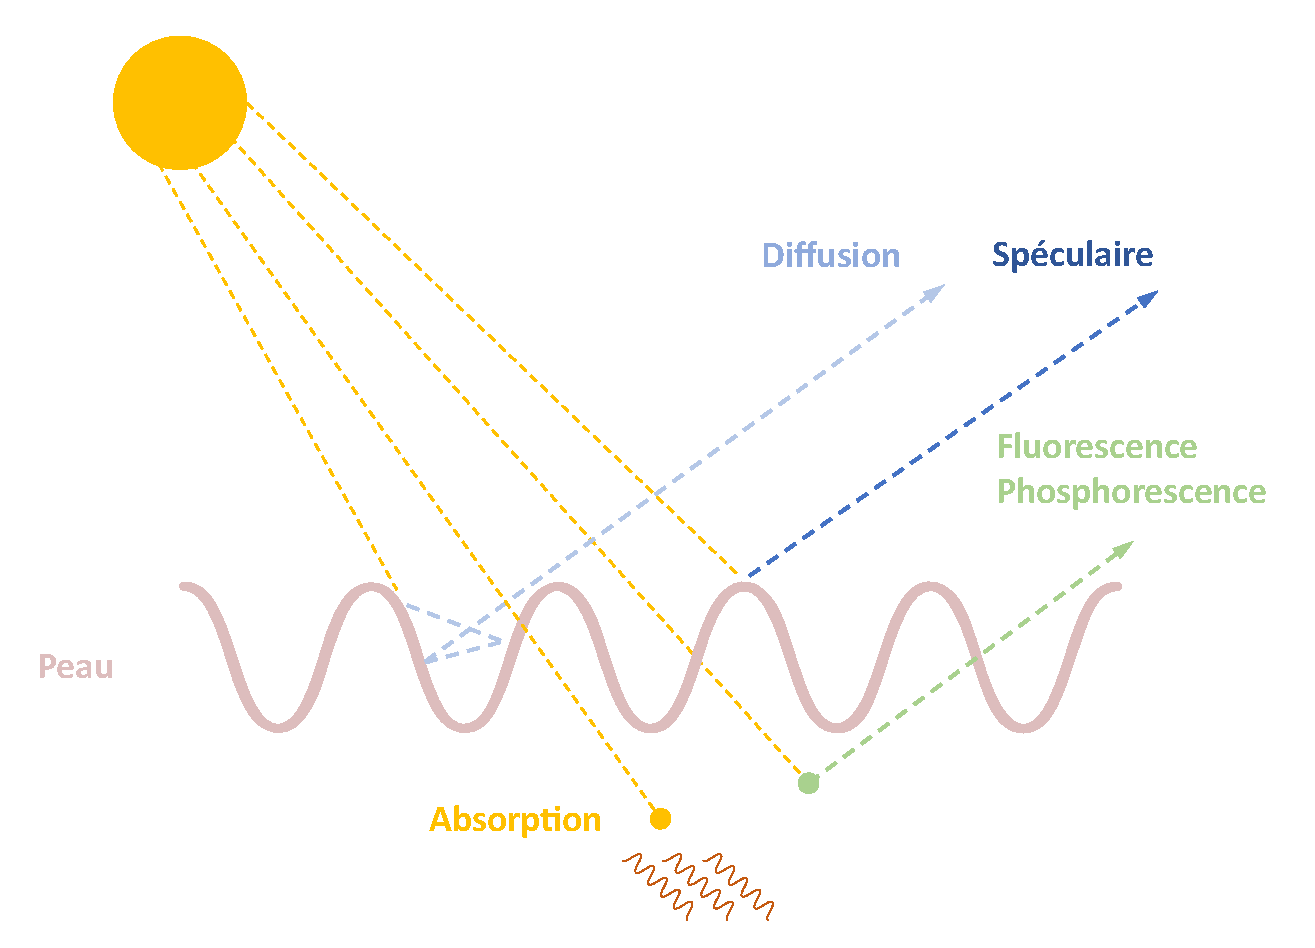
\includegraphics[width=\linewidth]{contents/chapter_2/resources/scheme_light_interaction.pdf}
    \caption{Schéma représentant les divers mécanismes d'interaction qui peuvent survenir suite à l'interaction de la lumière avec la peau. Ce sont ces divers phénomènes que les modalités optiques tentent d'exploiter pour extraire une information sur les tissus analysés.}
    \label{fig:scheme_light_interaction}
\end{figure}\par

Dans cette configuration, le choix de la source d'émission de lumière est l'un des points importants. En effet, comme démontré dans un travail précédent employant le principe de la \gls{led} en dermatologie~\cite{Barolet2008}, la longueur d'onde d'émission est l'un des paramètres d'influence possible quant à la profondeur des structures à observer dans la peau. Ainsi, des longueurs d'onde à l'entrée du spectre visible humain ($\approx$\SI{360}{\nano\metre}) ne parviennent pas à se frayer un chemin en profondeur et ne frôlent que les couches supérieures de l'épiderme, tandis que des longueur d'ondes plus élevées de ce même spectre ($\approx$\SI{780}{\nano\metre}) tendent à atteindre l'hypoderme et ses vaisseaux sanguins. Une synthèse de la pénétration de la lumière en fonction de la longueur d'onde est visible sur la \Cref{fig:scheme_light_penatrating}.\par

\begin{figure}[H]
    \centering
    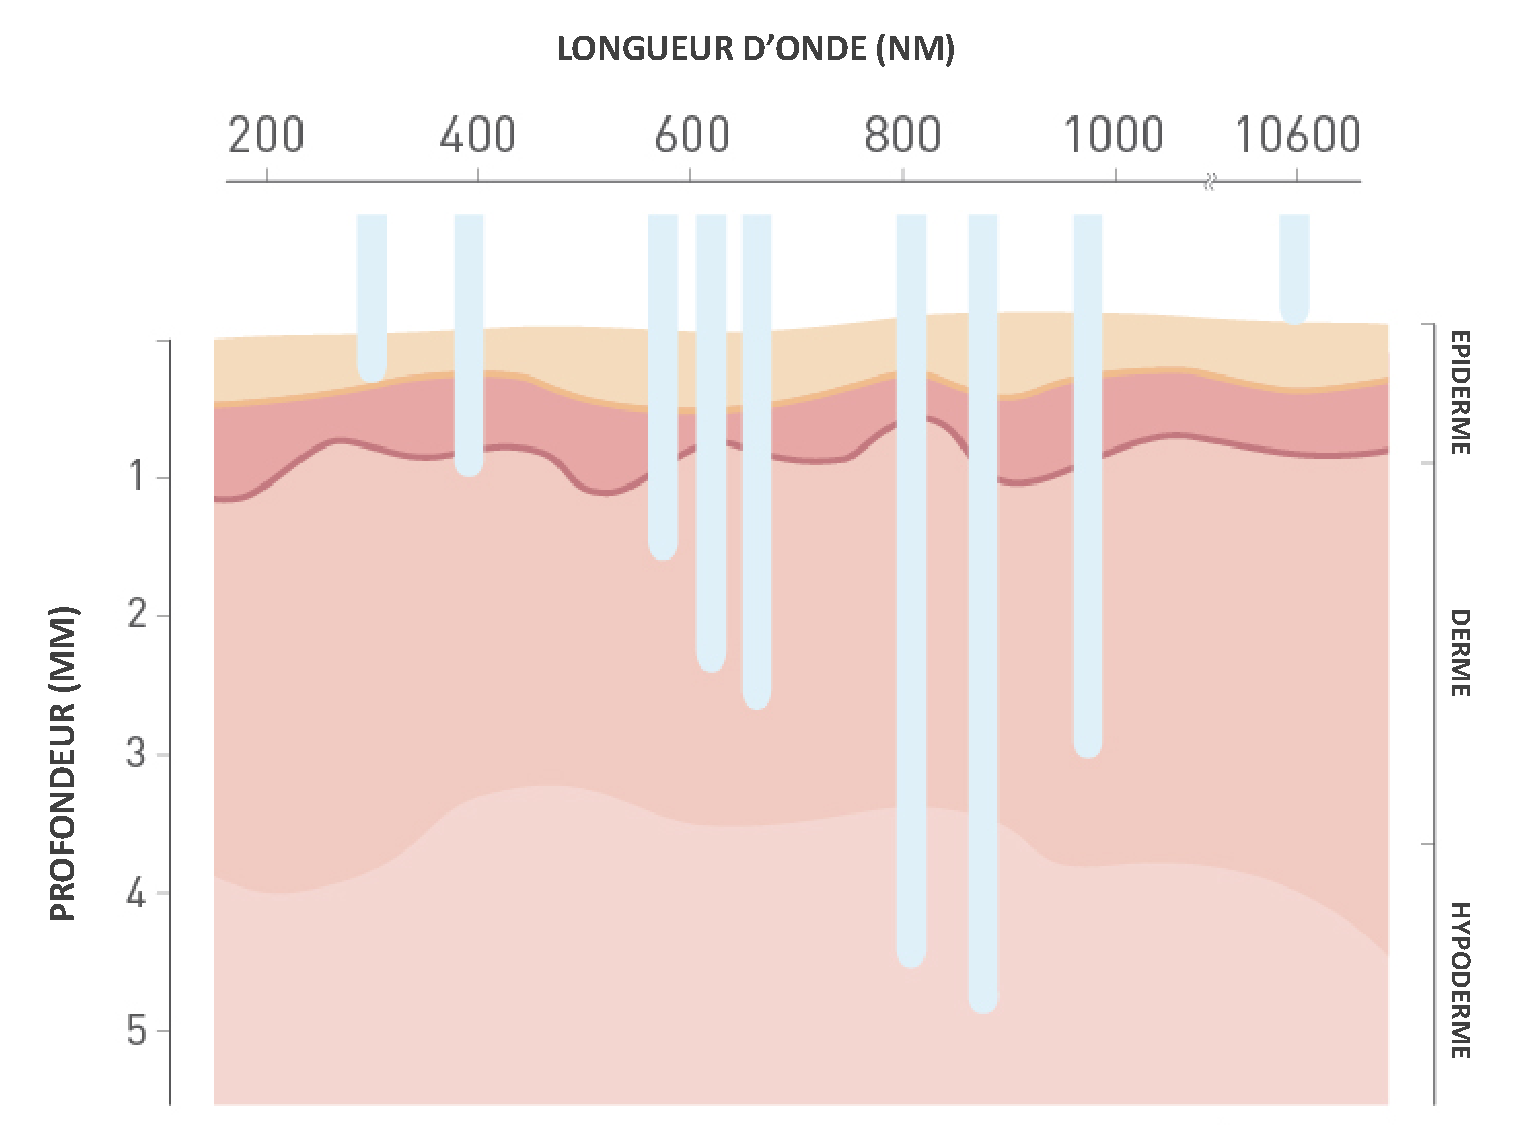
\includegraphics[width=0.8\linewidth]{contents/chapter_2/resources/scheme_light_penatrating.pdf}
    \caption{Schéma représentatif de la profondeur de pénétration (en mm) de la peau en fonction de la longueur d’onde de la lumière~\cite{Barolet2008}. Il s'agit d'un ordre de grandeur moyen constaté chez l'être humain, les propriétés de la peau varient d'un emplacement à un autre. Aucune information relative aux types de peaux étudiées, selon l'échelle de Fitzpatrick par exemple, n'a été mentionnée.}
    \label{fig:scheme_light_penatrating}
\end{figure}\par

Outre la question de la profondeur, le choix de la longueur d'onde permet d'interagir avec différents types de chromophores pouvant renseigner l'observateur sur des propriétés locales à la peau. Certains travaux focalisés sur les systèmes lasers et d'émission en général~\cite{Stewart2013} ont permis de mettre en avant le rapport entre la longueur d'onde et des composants majeurs de la peau tels que l'eau, l'hémoglobine (oxygénée ou non) ou la mélanine. Pour illustrer ce propos, la \Cref{fig:scheme_light_absorption} synthétise ce rapport entre la longueur d'onde d'émission et l'absorption associée aux principaux composants chromophores de la peau dont les quatre mentionnés. La quantification de ces composants peut présenter un intérêt dans la mesure où certaines pathologies peuvent altérer le métabolisme et donc modifier fondamentalement le ratio de chromophores présents, pouvant par exemple amener à une hypervascularisation. Certains travaux tentent ainsi de revenir à des fonctions de métabolisme~\cite{Im2016}.\par

\begin{figure}[H]
    \centering
    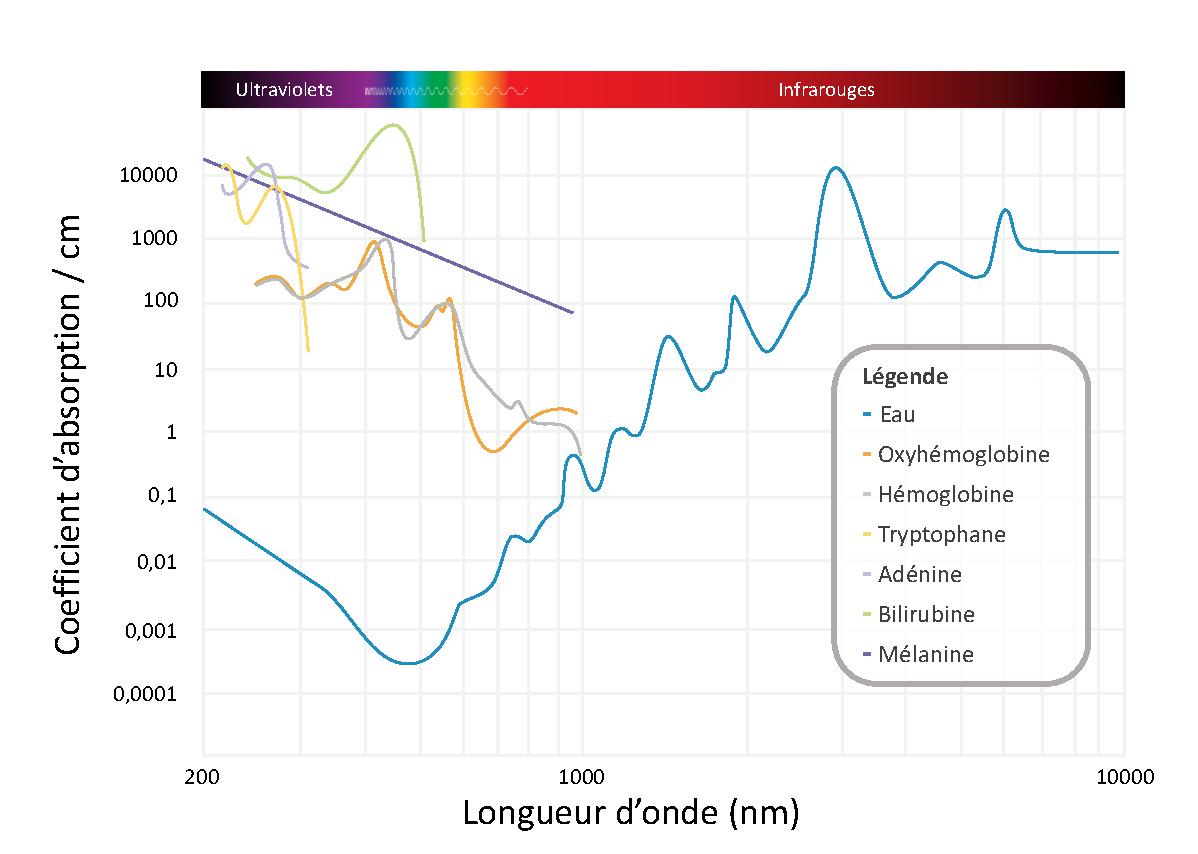
\includegraphics[width=\linewidth]{contents/chapter_2/resources/scheme_light_absorption.pdf}
    \caption{Représentation des coefficients d'absorption en fonction de la longueur d'onde pour les principaux composants chromophores présents dans la peau~\cite{Raulin2013}.}
    \label{fig:scheme_light_absorption}
\end{figure}
 
\clearpage

\section{Modalités d’imagerie non-invasives}
Afin de mieux suivre, voire de conserver une trace de leurs patients, les dermatologues disposent de nombreux outils. Ils peuvent entre autre dans leur pratique clinique se référer à divers types d’examens que nous distinguons au travers de deux catégories~:
\begin{itemize}
    \item D’une part \textbf{les examens dit non-invasifs}, c’est-à-dire ne provoquant pas de destruction des tissus du corps humain. Ces dispositifs sont capables de restituer une image de différente nature selon la nature du phénomène physique observé et ne provoquent en général pas d’inconfort particulier pour le patient. Ils peuvent représenter un investissement initial important mais s'amortissent assez bien sur le long terme. 
    \item D’autres part \textbf{les examens invasifs}, c’est-à-dire provoquant une effraction des tissus. L'histopathologie est le principal mode d'examen invasif et représente à ce jour le « gold standard » de ce domaine. Cet examen se réalise par biopsie, c'est à dire par prélèvement de tissus puis par une analyse histologique de ceux-ci. Cette technique peux être incommodantes pour le patient, requiert plus de temps qu'un examen non-invasif et est généralement plus coûteuses à l'unité.
\end{itemize}\par

Après avoir abordé de manière non exhaustive les principales pathologies de la peau et les principes d'interaction majeurs de la lumière avec la peau, il convient désormais d'aborder les diverses méthodes permettant une observation non invasive. Ces modalités d'imagerie franchissent en majorité le cap du numérique permettant un suivi plus aisé, voire un échange plus rapide entre professionnels, et l’utilisation de traitements automatiques. Nous séparons ces techniques en deux catégories distinctes~: d’une part les techniques de mesure optique et d'autre part les autres dispositifs basés sur une mesures physique indépendante de l'optique.\par

\subsection{Modalités par mesure optique}
Cette partie va nous permettre de décrire les principaux appareillages existants permettant l'observation des cellules de la peau. Évidemment, ces modalités sont également transposables à d'autres domaines d'applications que celui de la dermatologie. Nous ne traitons pas des dispositifs méconnus ou expérimentaux encore loin d'une application clinique car encore du domaine de la recherche clinique. La \Cref{tab:light_absorption} met en lumière ces dispositifs et leurs caractéristiques générales à but indicatif.\par
\begin{table}[H]
\begin{tabular}{lllll}
    \toprule
    \textbf{Technologie}                        & \textbf{Effet}    & \textbf{Résolution Spatiale} & \textbf{Profondeur}                \\ \hline
    Imagerie clinique                           & Réflectance       & Lentille dépendant           & \SIrange{0.1}{1}{\milli\metre}     \\
    Dermatoscopie                               & Réflectance       & Lentille dépendant           & \SIrange{0.1}{1}{\milli\metre}     \\
    Microscopie confocale par réflectance       & Réflectance       & \si{\micro\metre}            & \textless{} \SI{200}{\micro\metre} \\
    Tomographie en cohérence optique            & Réflectance       & \si{\micro\metre}            & \SIrange{1}{2}{\milli\metre}       \\
    Imagerie multispectrale                     & Réflectance       & Lentille dépendant           & \SIrange{0.1}{1}{\milli\metre}     \\
    Spectroscopie à réflexion                   & Réflectance       & Diamètre de la fibre         & \SIrange{0.1}{1}{\milli\metre}     \\
    Microscopie confocale Raman                 & Raman             & \si{\micro\metre}            & \SI{150}{\micro\metre}             \\
    \bottomrule
\end{tabular}
\caption{Aperçu des principales modalités de mesure optique actuelles en dermatologie, utilisées à but clinique ou à un stade de recherche clinique~\cite{Kollias2002}.}
\label{tab:light_absorption}
\end{table}\par

\subsubsection{Imagerie clinique}
L’examen de dépistage classique est associé en dermatologie à une inspection à l’œil nu exercée par une personne compétente ou sensibilisée à la détection de pathologies. Cette première modalité fait appel à un dispositif de photographie non propre à la dermatologie. Par ailleurs, elle constitue historiquement la première modalité de cette discipline mais également la moins onéreuse car emploie des caméras non propre à la discipline.\par

Cette modalité, avant l’avènement de l’informatique, se basait sur des supports de type argentique. L’évolution de ce matériel vers le numérique, et l’arrivée de systèmes de type \gls{pacs} ont conjointement motivé une transition vers des données dématérialisées.\par

Ce type d’imagerie donne à l’observateur un point de vue subjectif, similaire à une observation à l’œil nu, utile dans le cadre d’un diagnostic à distance ou dans le suivi à long terme d’un patient. Néanmoins, l'un des points faibles est le manque de standard concernant le format d'image et de protocole concernant l'acquisition des images~: pas de contraintes d'éclairage, ni de contraintes sur le point de vue à adopter au moment de la prise d'image. Ces éléments amènent à une grande diversité de données, comme nous pouvons le voir sur la \Cref{fig:example_photography}.\par

\begin{figure}[H]
\centering
    \begin{subfigure}{.45\textwidth}
      \centering
      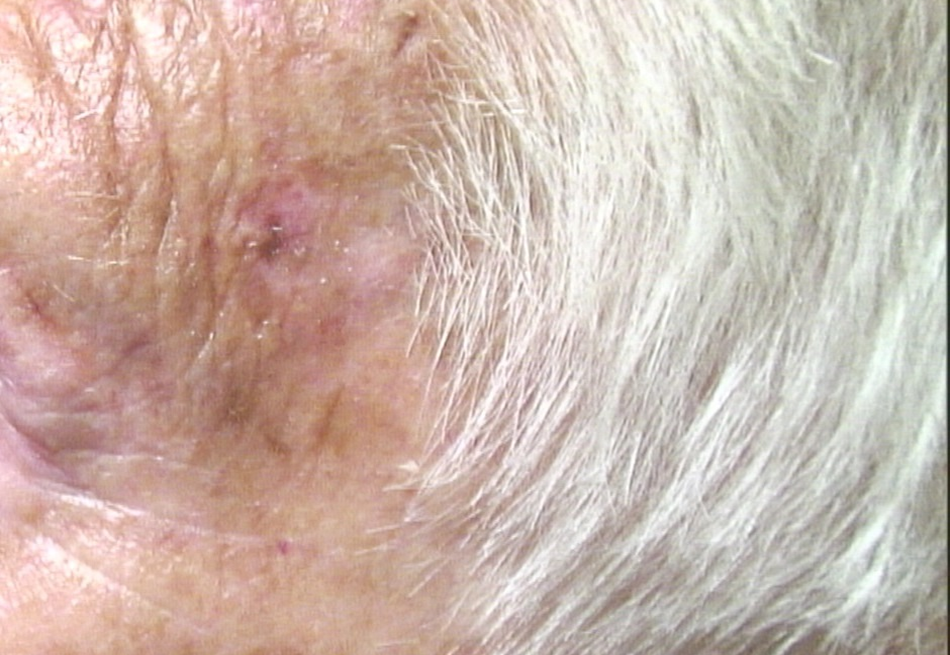
\includegraphics[width=\linewidth]{contents/chapter_2/resources/example_photography_1.png}
    \end{subfigure}
    \begin{subfigure}{.45\textwidth}
      \centering
      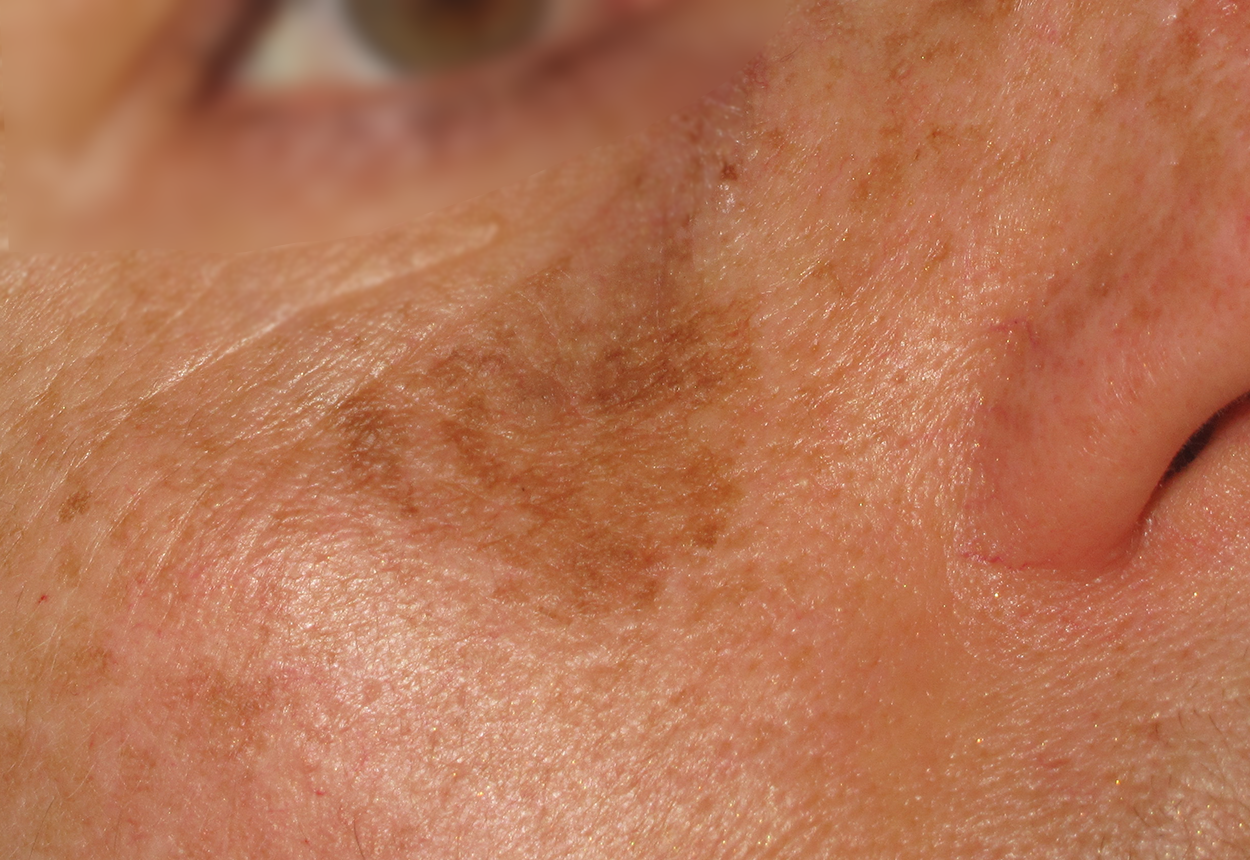
\includegraphics[width=\linewidth]{contents/chapter_2/resources/example_photography_2.png}
    \end{subfigure}
    \caption{Exemple d'images dites de photographie clinique. Ces deux exemples donnent un aperçu de la diversité des acquisitions en terme d'exposition, d'angle de vue et de résolution d'image.}
    \label{fig:example_photography}
\end{figure}\par

Ces dernières années ont vu l'émergence de nouveaux types d'appareillages qui étendent la photographie clinique au corps entier. Ces appareils permettent une traçabilité et un suivi des lésions apparentes sur le corps d'un patient. En effet, l'un des meilleurs critères du suivi de lésions dans le dépistage de maladies, tel que le mélanome, reste l'évolution au cours du temps de ces lésions. Cet élément a notamment été mis en avant en 2004, et est encore considéré de nos jours comme l'un des critères majeurs~\cite{Abbasi2004,Glazer2017}. Différents industriels commercialisent des dispositifs de plus en plus performants dont FotoFinder et son système ATBM mais également la société Pixience avec le "Body-Mapper®" permettant ce suivi ainsi qu'un contrôle de l'éclairage lors de la prise de vue. Une interface guide le médecin lors de la prise d'images et permet d'associer à un modèle humain les diverses parties du corps (voir la \Cref{fig:example_device_bodymapper}).\par

\begin{figure}[H]
\centering
    \begin{subfigure}{.28\textwidth}
      \centering
      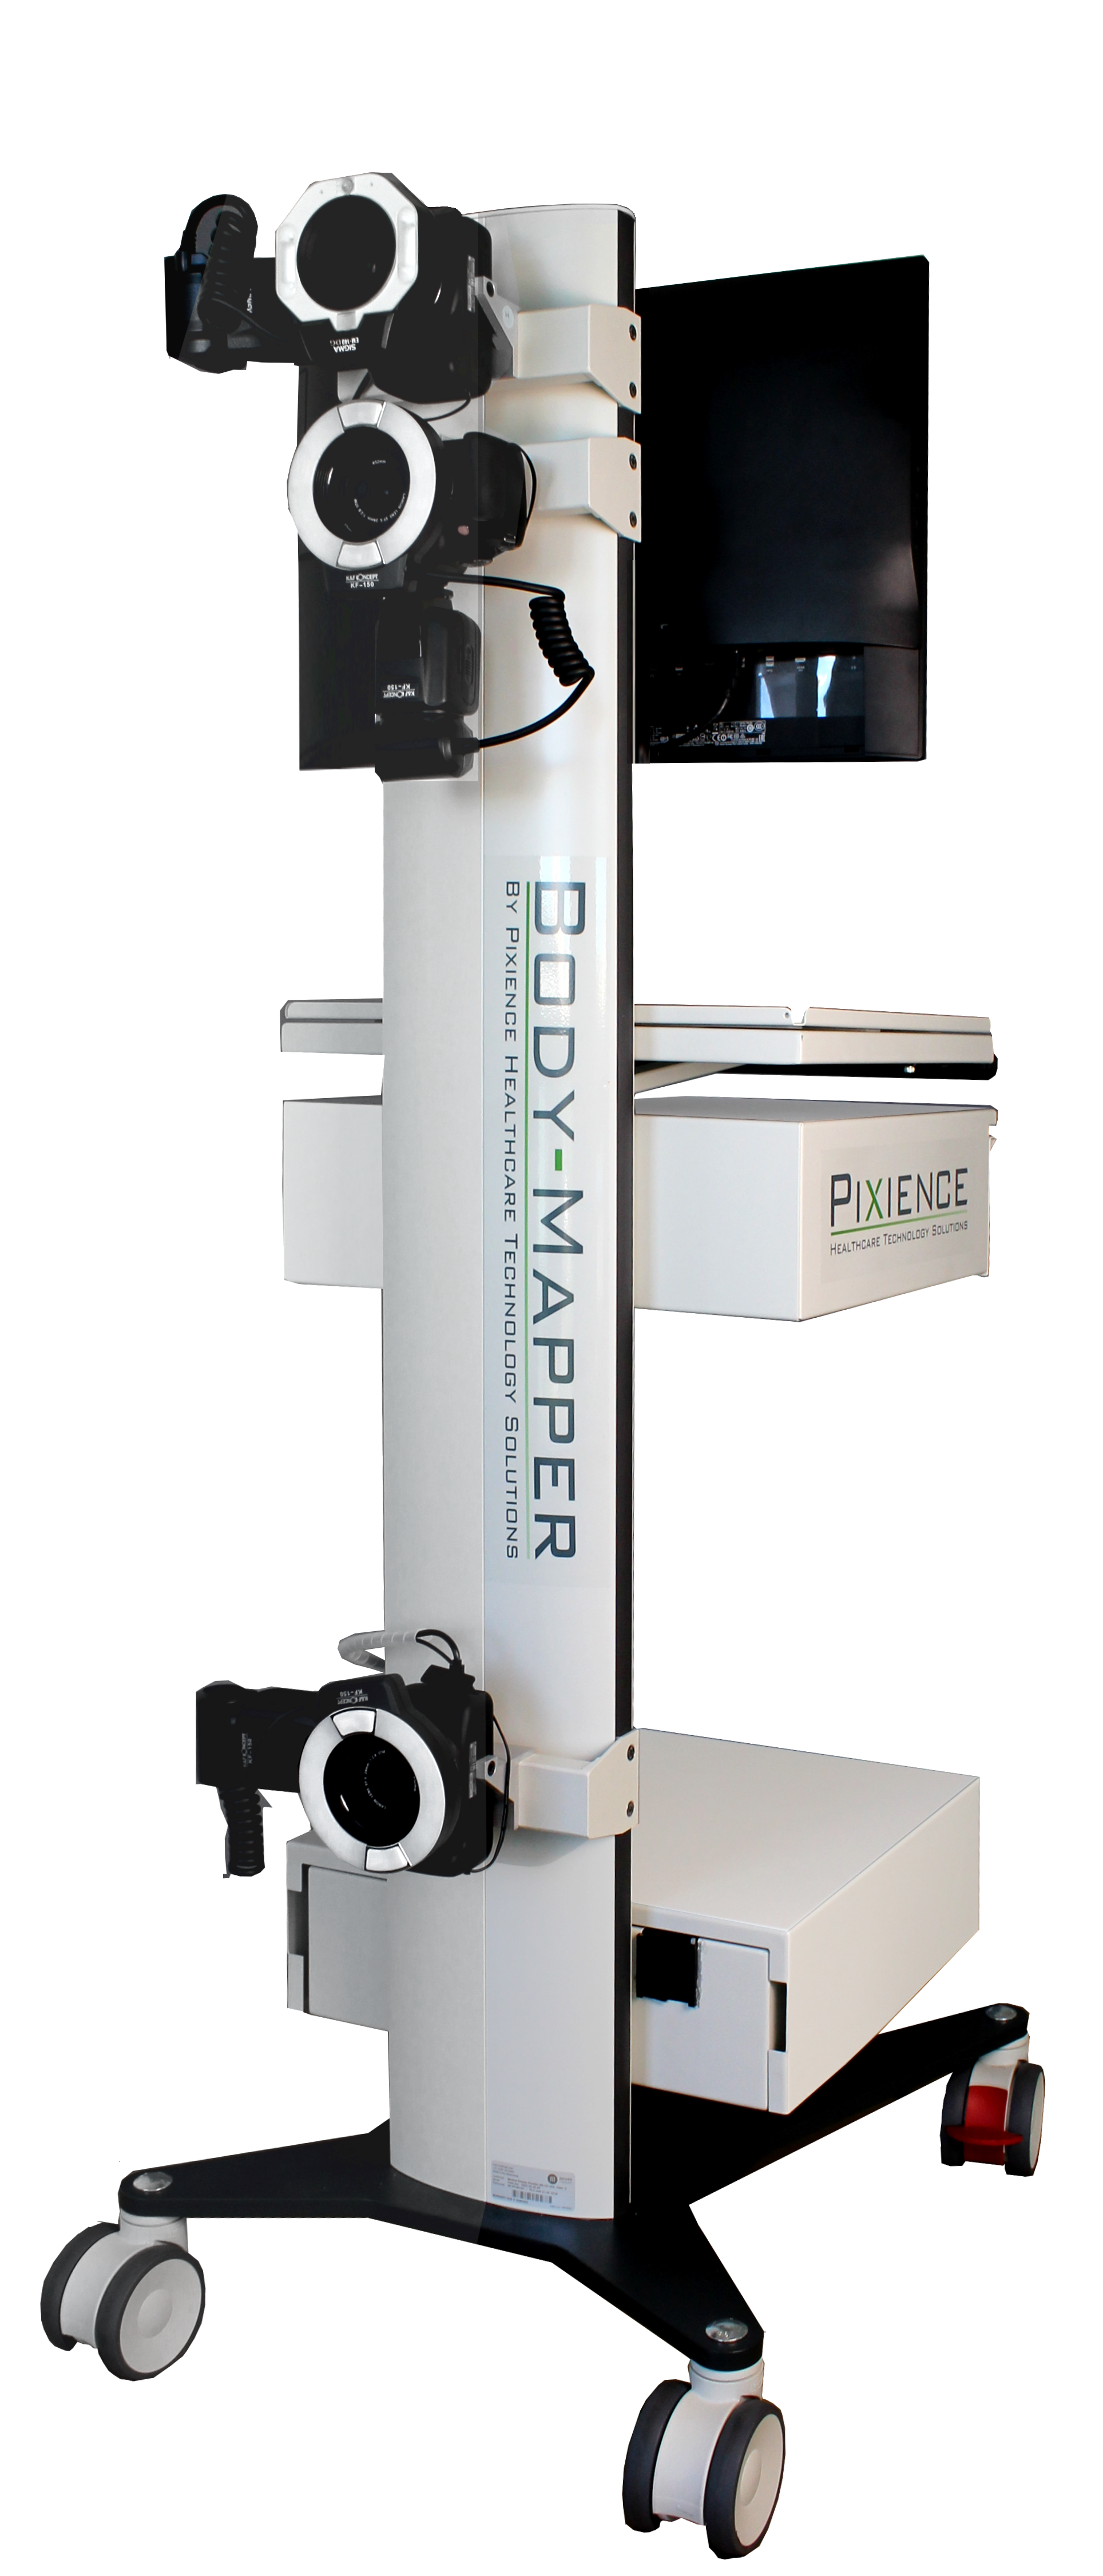
\includegraphics[width=\linewidth]{contents/chapter_2/resources/example_device_bodymapper_1.png}
    \end{subfigure}
    \begin{subfigure}{.65\textwidth}
      \centering
      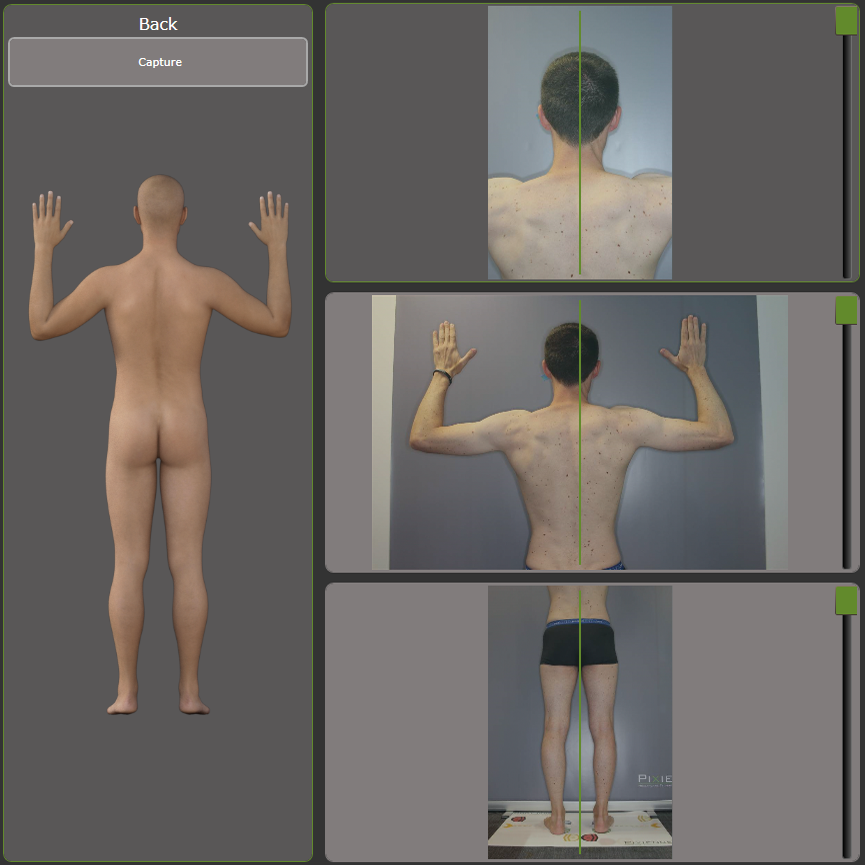
\includegraphics[width=\linewidth]{contents/chapter_2/resources/example_device_bodymapper_2.png}
    \end{subfigure}
    \caption{Exemple du Body-Mapper, un appareil de photographie clinique corps entier, proposé par Pixience. A gauche, l'appareil d'acquisition ; A droite, son interface logicielle permettant d'acquérir les diverses partie du corps.}
    \label{fig:example_device_bodymapper}
\end{figure}\par


\subsubsection{Dermatoscopie}
Également appelé dermoscopie, microscopie en épiluminescence ou encore microscopie de surface, ce dispositif permet d’observer les lésions cutanées. Nous préférons le terme de dermatoscopie pour la suite de ce manuscrit. Cette technique d’imagerie est partiellement attribuée à Johan Christophorus Kohlhaus dont les travaux menés, au XVIIème siècle, sur la microscopie de surface, auraient grandement contribué à initier cette modalité. Les premiers dispositifs ont émergés en 1971~\cite{MacKie1972}, et ce sont les années 1980 qui ont contribué à son essor chez un grand nombre de praticiens.\par

Cet outil possède comme première caractéristique, de réduire les réflexions de lumière et contribue à rendre le stratum corneum translucide~\cite{Katz2001}, permettant ainsi au praticien de visualiser les couches sous-jacentes~: épiderme, jonction derme/épiderme ou encore le derme papillaire non visible à l’œil nu. Cette réflexion de lumière était initialement supprimée par l’utilisation d’un fluide (eau, gel, …) entre la peau et la lentille du dispositif (dermatoscope non polarisé). De récentes améliorations ont permis de rendre l'utilisation d'un fluide obsolète par l'utilisation de lumière polarisée (dermatoscope polarisé). Un premier filtre, polarisé horizontalement, est disposé juste après la source de lumière, puis un second filtre, polarisé verticalement, est mis en place avant le capteur/fenêtre de visée (voir \Cref{fig:scheme_polarized_dermoscopy}). Ce dispositif permet ainsi de s'affranchir de la lumière spéculaire directement issue de la source de lumière qui parasite l'observation~\cite{Campos-do-Carmo2008}.\par

\begin{figure}[H]
\centering
    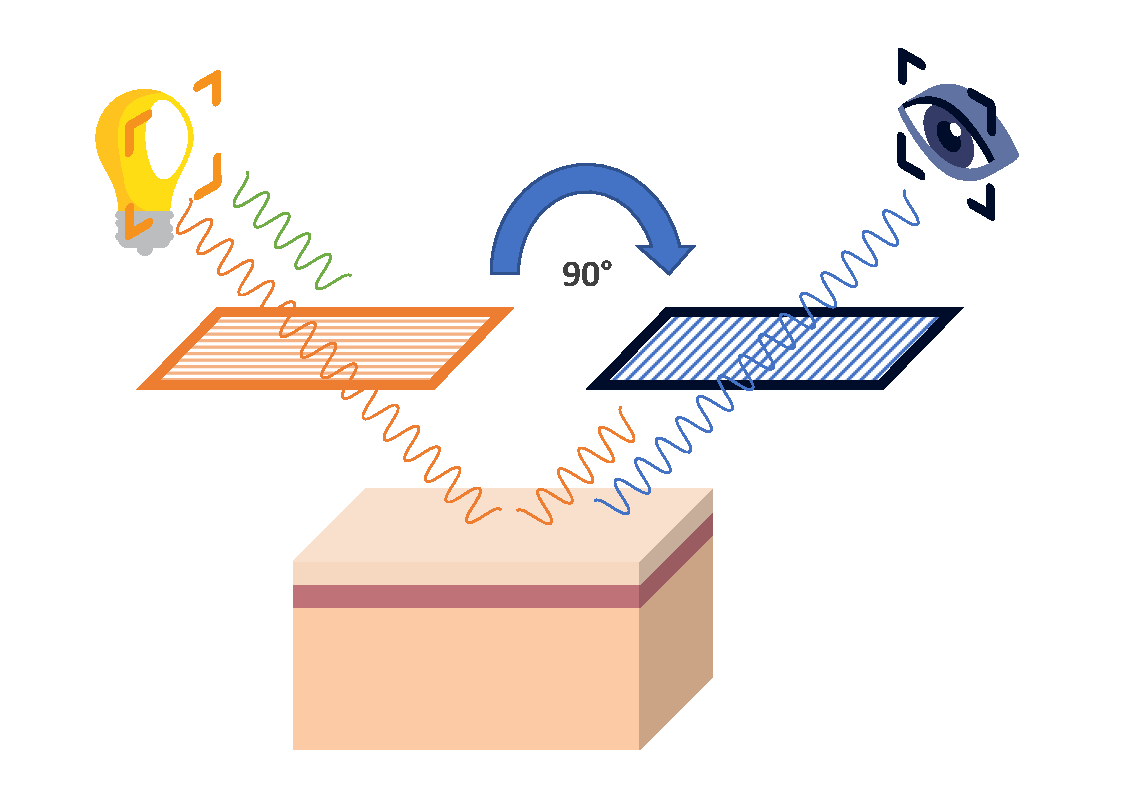
\includegraphics[width=0.7\linewidth]{contents/chapter_2/resources/scheme_polarized_dermoscopy.pdf}
    \caption{Principe de dermatoscope à lumière polarisée. Un filtre est disposé après la source de lumière, puis un second dont la polarisation est perpendiculaire au premier juste avant la fenêtre d'observation~\cite{sonthalia2019}.}
    \label{fig:scheme_polarized_dermoscopy}
\end{figure}\par

Une seconde caractéristique non négligeable, est la mise à disposition d’un zoom permettant de grossir en lumière blanche jusqu'à 150 fois selon la complexité des modèles proposés \cite{Campos-do-Carmo2008}. Cette dernière caractéristique octroie au praticien la possibilité d’appréhender au mieux la structure dans ses moindres détails.\par

De plus, son faible coût d’achat, sa rapidité de diagnostic et son efficacité en comparaison avec le seul œil humain \cite{Lallas2013} contribuent largement à sa démocratisation dans la profession. Bien qu’utilisée majoritairement dans le dépistage de lésions pigmentaires, son efficacité semble avérée dans le cas de lésions dites non pigmentaires (\gls{bcc} et \gls{scc}) \cite{Lallas2013}. 

Ces dispositifs tendent à s'adapter de plus en plus aux besoins de leur marché, en proposant par exemple une caméra haute résolution et permettant une utilisation polyvalente de l'appareil avec un connecteur générique comme le propose Pixience (voir la \Cref{fig:example_device_ccube}). Leur appareil a permis la mise en avant de lésions chez la souris et l'homme~\cite{Cinotti2016,Pillon2017}. D'autres sociétés comme Dermlite proposent une solution plus nomade et adaptable aux principaux appareils du marché, dont le principal dispositif est visible sur la \Cref{fig:example_device_dermlite}.\par

\begin{figure}[H]
    \centering
    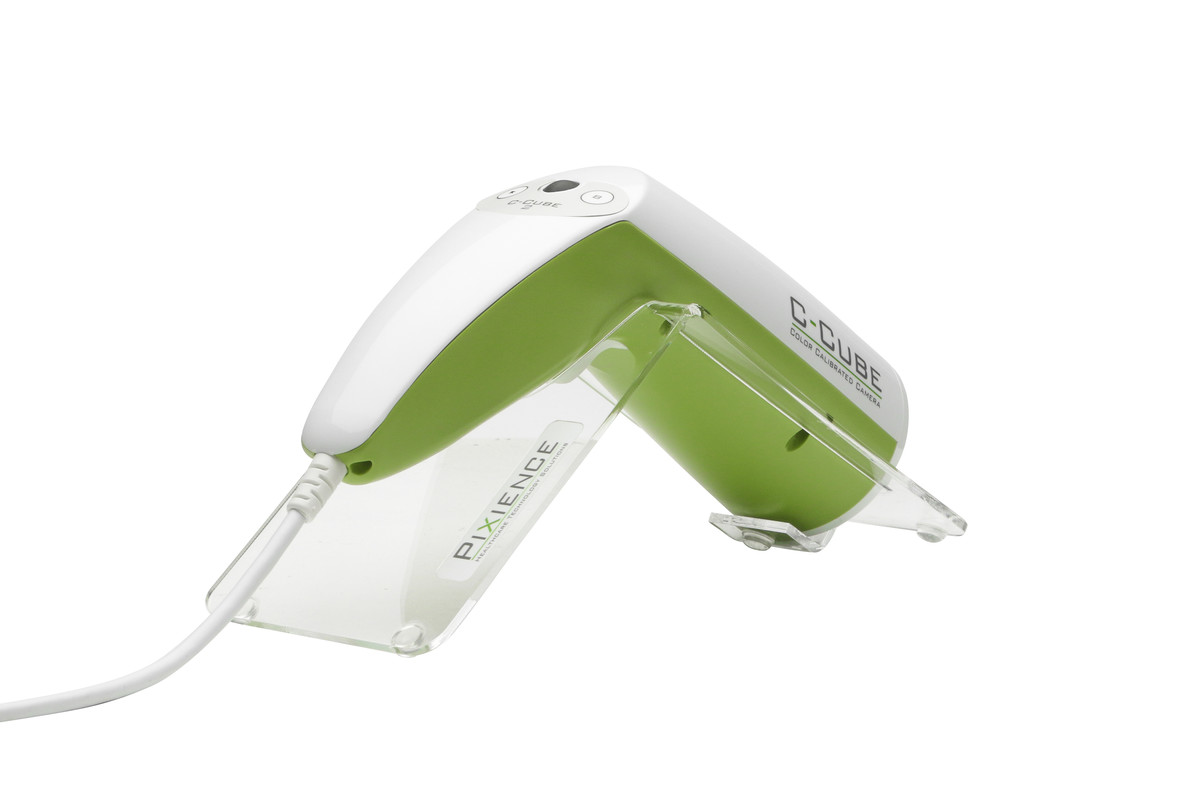
\includegraphics[width=0.50\linewidth]{contents/chapter_2/resources/example_device_ccube.jpg}
    \caption{Exemple du dermatoscope C-Cube proposé par la société Pixience.}
    \label{fig:example_device_ccube}
\end{figure}\par

\begin{figure}[H]
\centering
    \begin{subfigure}{.32\textwidth}
      \centering
      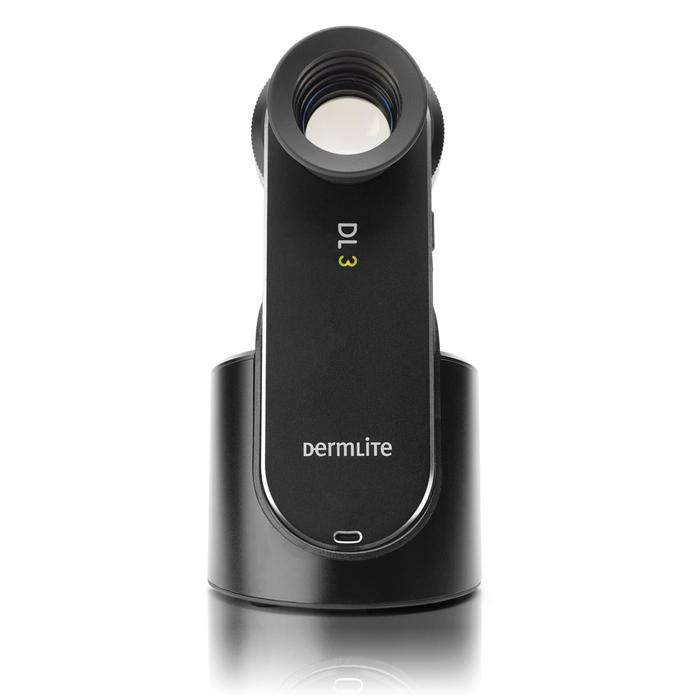
\includegraphics[width=\linewidth]{contents/chapter_2/resources/example_device_dermlite_1.png}
    \end{subfigure}
    \begin{subfigure}{.32\textwidth}
      \centering
      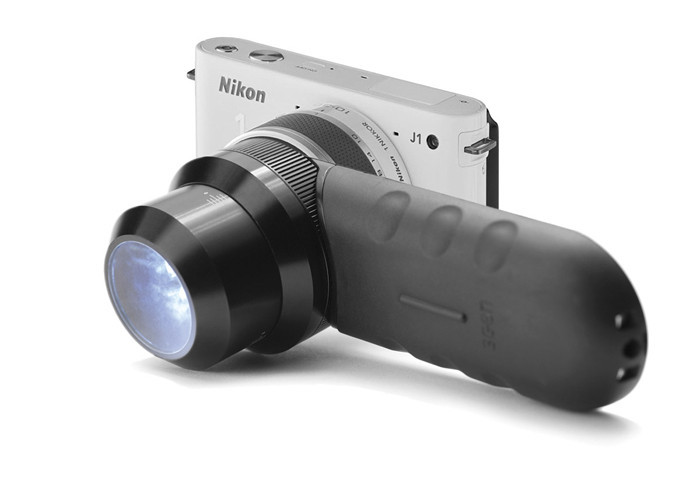
\includegraphics[width=\linewidth]{contents/chapter_2/resources/example_device_dermlite_2.png}
    \end{subfigure}
    \begin{subfigure}{.32\textwidth}
      \centering
      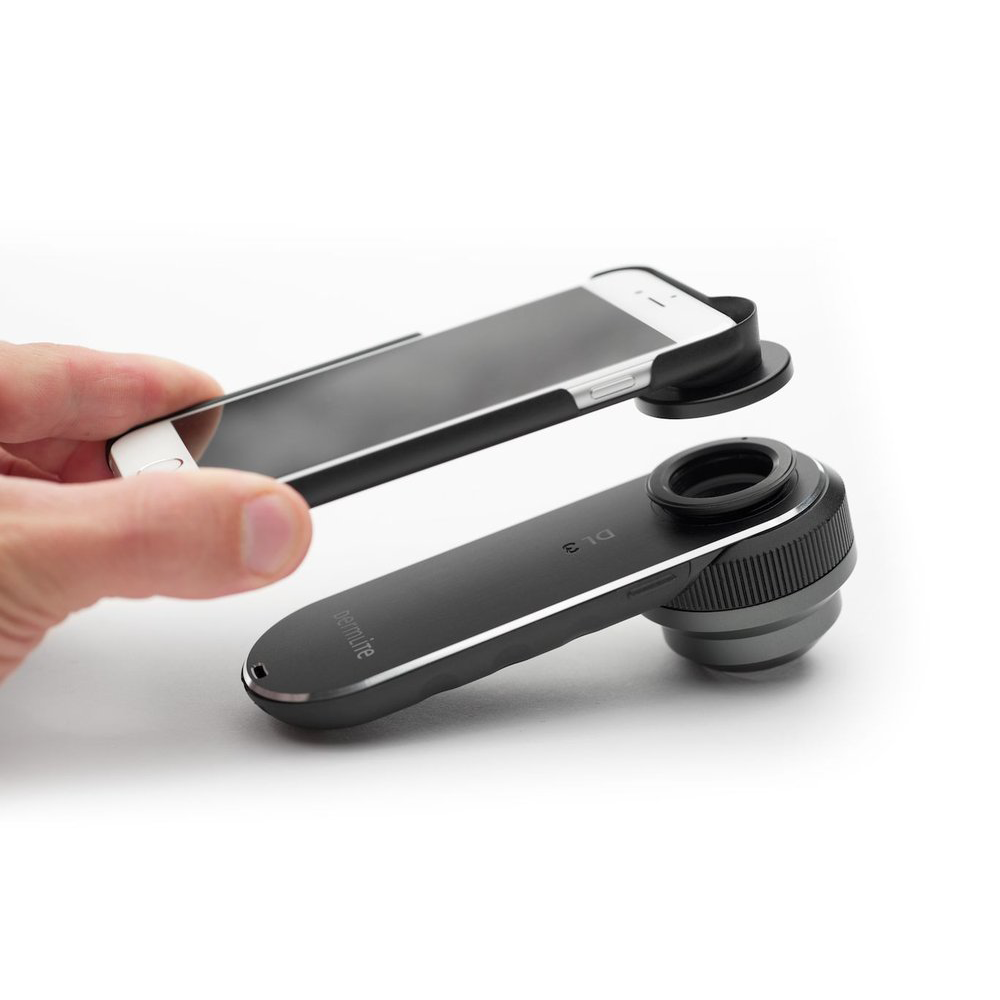
\includegraphics[width=\linewidth]{contents/chapter_2/resources/example_device_dermlite_3.png}
    \end{subfigure}
    \caption{Exemple de dermatoscope proposé par la société Dermlite. A gauche, le dispositif seul ; Au milieu, ce même dispositif adapté à un appareil photo standard ; A droite, le dispositif adapté à une caméra de téléphone portable.}
    \label{fig:example_device_dermlite}
\end{figure}\par

\subsubsection{Microscopie confocale par réflectance}
La \acrfull{rcm} est une technique d’imagerie décrite durant les années 1950 par Marvin Minsky~\cite{Sheppard2019}. Les avancées réalisées durant les années 1990 ont permis de réduire considérablement la taille de cet appareil et de faciliter ainsi son utilisation dans divers domaines. Cette technique de plus en plus répandue dans les services de dermatologie a également connu un regain de notoriété dans les journaux scientifiques~: une recherche à l’aide des mots clés « reflectance confocal microscopy skin » apporte une dizaine de publications vers les années 2000 contre un moyenne de 1500 chaque année depuis 2010~\textsuperscript{\ref{footnote:scholar_rcm}}.\par

\addtocounter{footnote}{1}
\footnotetext[\thefootnote]{Source~: Google Scholar. \label{footnote:scholar_rcm}}

\begin{figure}[H]
\centering
    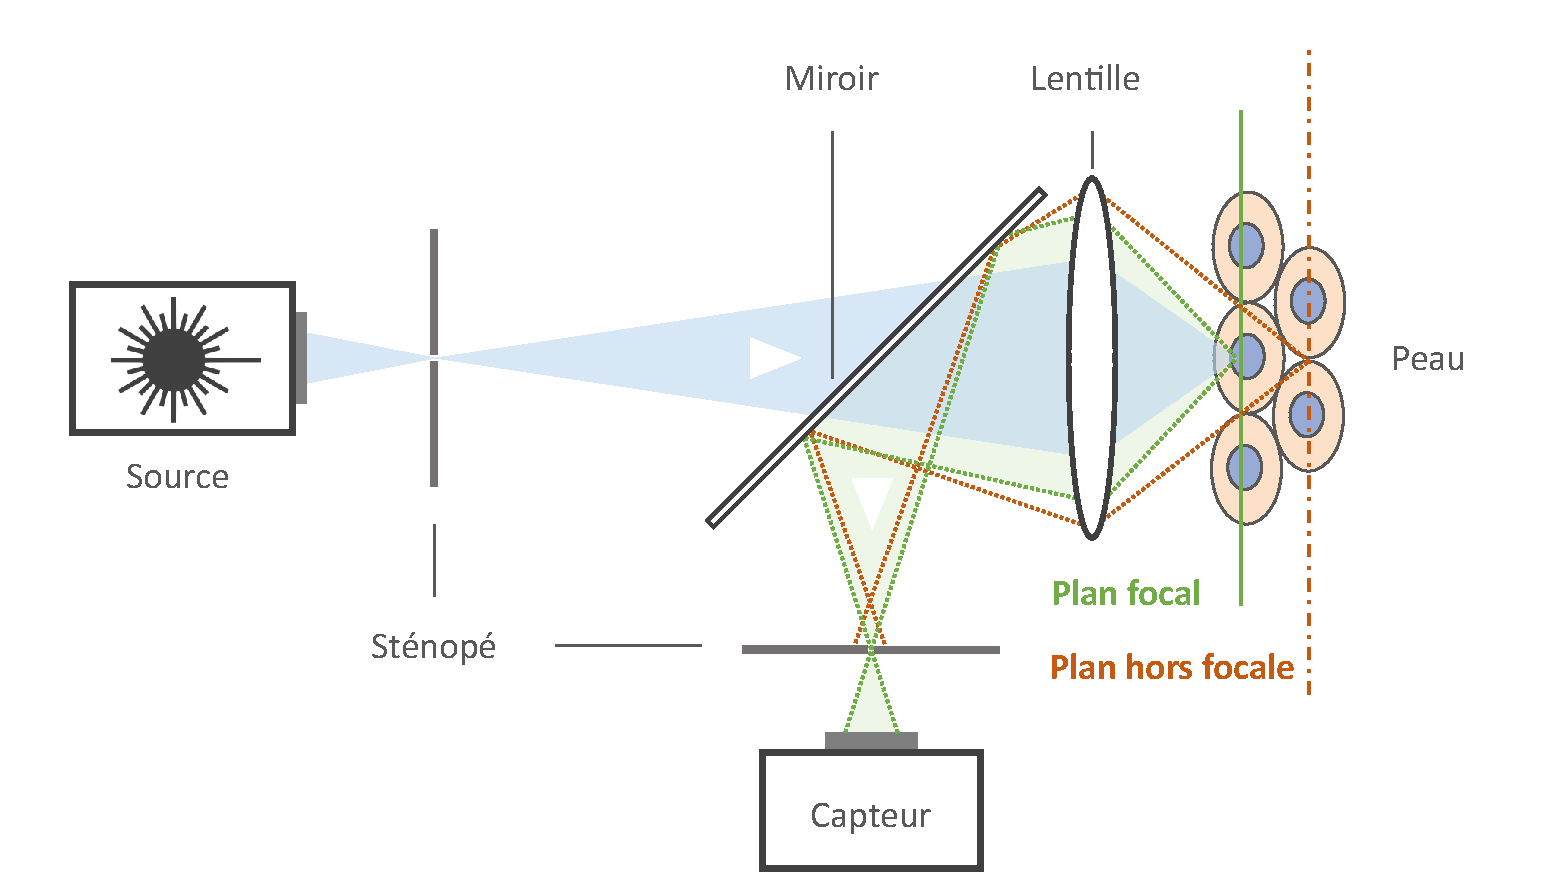
\includegraphics[width=0.9\linewidth]{contents/chapter_2/resources/scheme_principle_rcm.pdf}
    \caption{Schéma de fonctionnement du \gls{rcm} par Marvin Minsky. Une source de lumière est émise et focalisée en un point spécifique de la peau puis la lumière est réfléchie et reçue par une caméra au travers d'un sténopé (trou de faible diamètre). La lumière hors focale est ainsi arrêtée.}
    \label{fig:scheme_principle_rcm}
\end{figure}\par

Cette technique emploie l’utilisation d’un sténopé situé devant le capteur et permet de conserver uniquement les photons issus du plan focal choisi, illustré en \Cref{fig:scheme_principle_rcm}. Nous pouvons par ce principe, obtenir différents plans focaux ou plans de coupes, participant à l’obtention d’une information 3D~\cite{Sheppard2019}. En dermatologie, les dispositifs se basent sur des longueurs d’ondes de \SI{830}{\nano\metre} non invasives pour la peau et les yeux, mais limitent la profondeur du dispositif à \SIrange{200}{300}{\micro\metre}.\par

Pour finir, à la manière du dermatoscope, un gel à base d’eau de réfraction proche de celle de l’épiderme est utilisé entre la lentille du microscope et la peau afin de limiter la perte de photons et de permettre l’obtention d’images du derme.\par

\subsubsection{Tomographie en cohérence optique}
Initialement conçue pour le domaine de l’ophtalmologie, la \gls{oct} est une technologie récente qui tend à se démocratiser à de nombreux domaines d’intervention dont celui de la dermatologie. Ces dispositifs se basent sur un principe d’interférométrie, préalablement utilisé pour les dispositifs dits d’interférométrie à faible cohérence temporelle fournissant une information à une dimension. Le principe consiste à utiliser une source de lumière commune divisée en deux faisceaux, l’un servant de référence et le second servant à l’analyse de l’échantillon considéré. Le faisceau de référence possède un miroir ajustable, permettant de modifier sa distance parcourue et définissant ainsi la profondeur d’échantillon analysable. En effet, deux faisceaux peuvent interférer si la distance parcourue (et leur déphasage) est identique comme représenté dans la \Cref{fig:scheme_principle_oct}.\par

Le \gls{oct} est une extension de ce principe à deux dimensions, permettant la caractérisation d’une « tranche » de tissu. Cette modalité d’imagerie propose ainsi une information temps réel en profondeur (de l’ordre du millimètre), avec une résolution proche du micromètre. Nous pouvons obtenir, par acquisition de plusieurs plans de coupe, une reconstruction de la peau et de ses structures.\par

\begin{figure}[H]
    \centering
    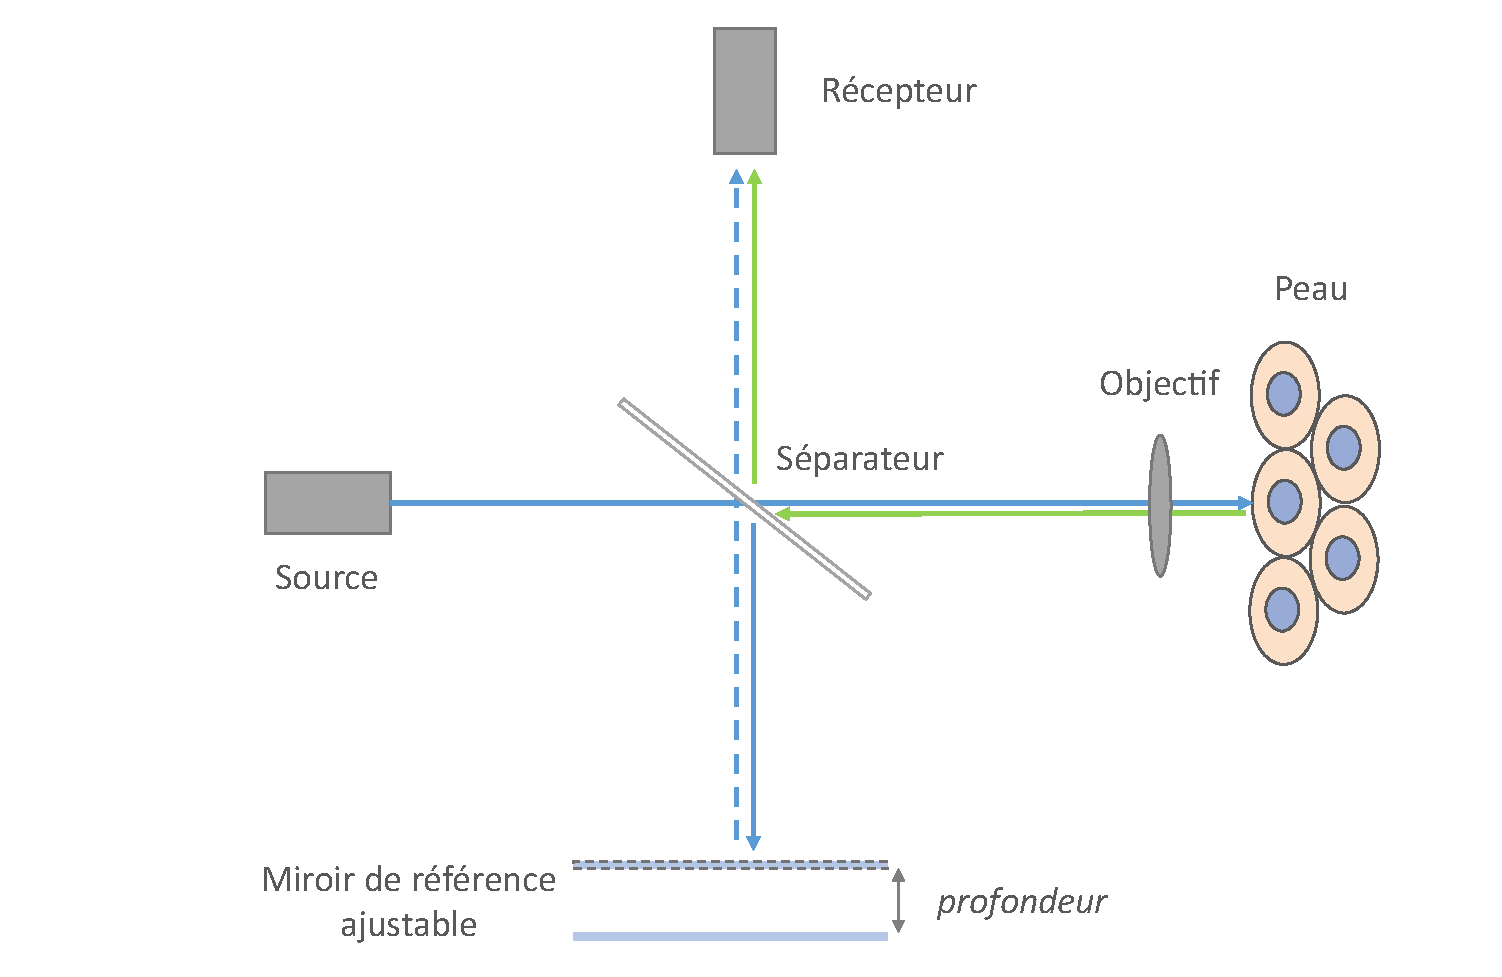
\includegraphics[width=0.8\linewidth]{contents/chapter_2/resources/scheme_principle_oct.pdf}
    \caption{Schéma de fonctionnement du \gls{oct}.}
    \label{fig:scheme_principle_oct}
\end{figure}\par

\subsubsection{Spectroscopie par réflectance}
La spectroscopie de réflectance peut être assimilée à l'imagerie multispectrale dans le sens ou elle fournit également une information de spectre à un même instant, c'est à dire contenant plusieurs valeurs numériques, chacune propre à une longueur d'onde spécifique. Néanmoins ce principe diffère en plusieurs points~: l'information fournie est propre à un unique point de l'espace et est obtenue en temps réel.\par

Pour cela, une source de lumière stable dans le temps, uniforme et couvrant l'ensemble du spectre que l'on désire observer est utilisée. Cette lumière est ensuite canalisée au sein d'une ou plusieurs fibres optiques afin d'être conduite jusqu'à l'échantillon supposé. Le phénomène de réflectance de l'échantillon est ensuite capté à l'aide d'une ou plusieurs fibres optiques jusqu'à un spectromètre qui va dissocier le signal (phénomène de diffraction), afin de cibler de multiples cellules présentes sur un capteur numérique~\cite{Murphy2005,Malla2008}\textsuperscript{\ref{footnote:aventes_spectrometer}}.\par

Ces capteurs font l'objet d'une procédure de calibration à l'aide de pantones ou nuanciers dont les propriétés visuelles sont établies, comme le propose par exemple le ColorChecker\textsuperscript{®}~\textsuperscript{\ref{footnote:colorchecker}}. En effet, il est nécessaire d'empêcher une saturation du signal conduisant à une perte d'information tout en exploitant au mieux la quantification octroyée par le capteur. Sa nécessité est le fruit des multiples conditions d'éclairage possibles de l'environnement mais également de la variété des sources de lumière pouvant être employées avec ce type de dispositif. Cette étape permet ainsi de rectifier et compenser le signal "idéal".\par

\begin{figure}[H]
    \centering
    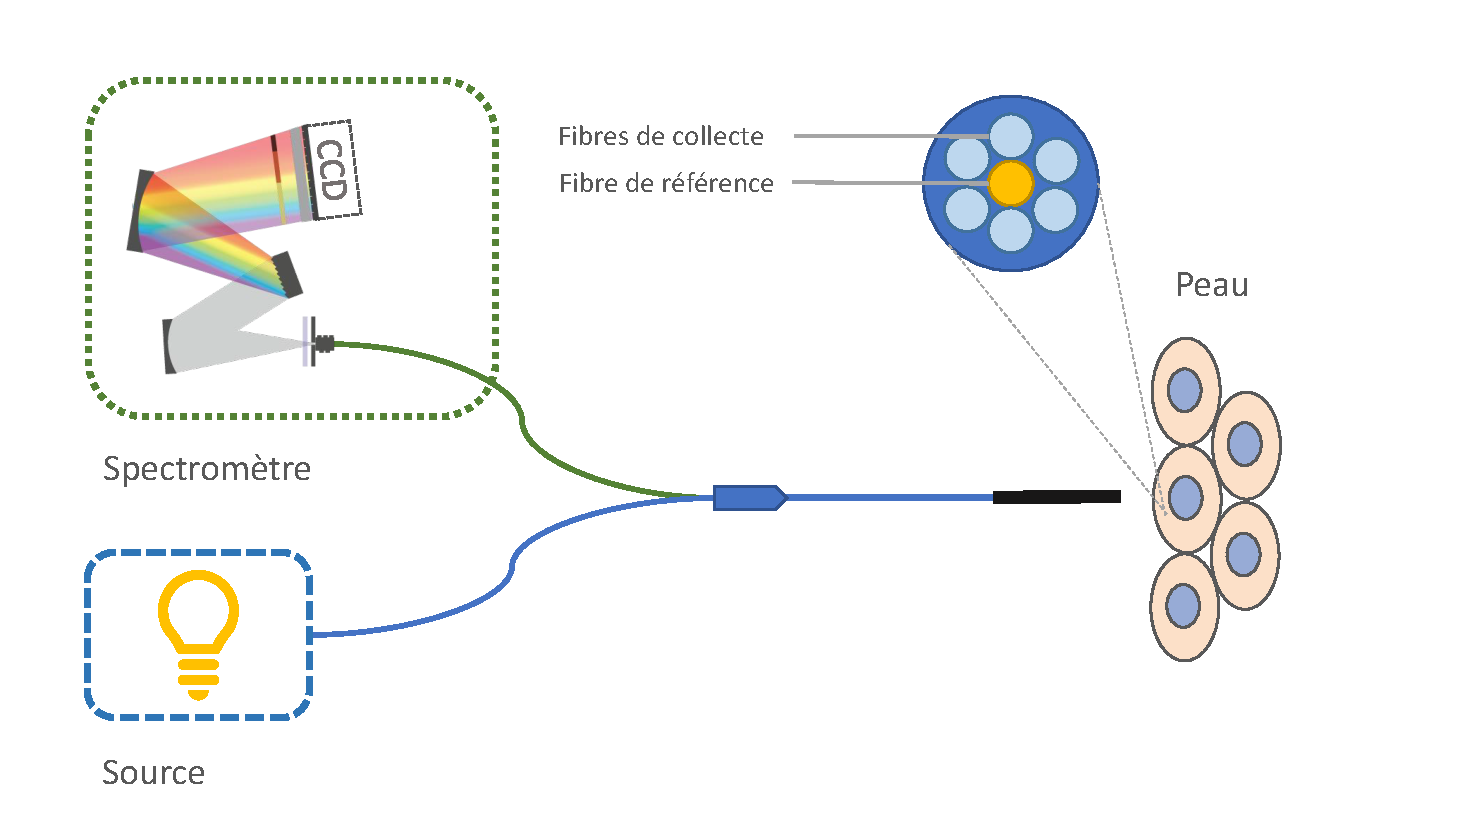
\includegraphics[width=\linewidth]{contents/chapter_2/resources/scheme_principle_spectroscopy.pdf}
    \caption{Schéma représentant le fonctionnement d'un spectroscope par réflectance. Une lumière de référence est générée puis acheminée jusqu'à la zone cible. Cette lumière transite le long d'une ou plusieurs fibres optiques. Puis le phénomène de réflectance est capté et envoyé au spectromètre par le biais d'une ou plusieurs fibres. Le signal reçu est ensuite décomposé puis envoyé à la surface d'un capteur numérique.}
    \label{fig:scheme_principle_spectroscopy}
\end{figure}\par

\addtocounter{footnote}{1}
\footnotetext[\thefootnote]{Source~: Spectromètres AvaSpec\textsuperscript{®}, Avantes, Pays-Bas. \label{footnote:aventes_spectrometer}}

\addtocounter{footnote}{1}
\footnotetext[\thefootnote]{Source~: X-Rite, ColorChecker\textsuperscript{®}, Michigan, États-Unis. \label{footnote:colorchecker}}

\subsubsection{Imagerie multispectrale}
L'imagerie multispectrale est un principe d'imagerie dans lequel les pixels contenus dans une image ne se résument pas une ou trois valeurs (respectivement pour une image en intensités ou RGB), mais à une multitude de valeurs décrivant chacune une longueur d'onde. Ce nombre de valeurs (ou échantillonage) spectral est ainsi dépendant de la précision recherchée dans un domaine d'application particulier. Ces dispositifs sont séquentiels, même si les temps d'acquisition entre les diverses valeurs tendent à se réduire fortement avec les évolutions technologiques. Différents principes sont mis en oeuvre pour parvenir à l'obtention de ces images, visible sur la \Cref{fig:scheme_multispectral_principle}. Nous retiendrons les principes suivants~:
\begin{itemize}
\item par modification \textbf{de la source émettrice de lumière}, soit en utilisant des \gls{led} programmables ou soit des combinaisons de filtres (il peut s'agir de filtres programmables) permettant de modifier les propriétés de la lumière,
\item par filtrage \textbf{de la lumière reçue}, bien souvent à l'aide de combinaison de filtres (il peut s'agir de filtres programmables) permettant de choisir les longueurs d'ondes désirées. Des capteurs multicouches émergent permettant une acquisition quasiment simultanée de l'information sur le capteur en lui-même~\textsuperscript{\ref{footnote:foveon_sensor}}.
\end{itemize}\par

Ce principe à ainsi pour but de revenir à une information plus riche, que celle transmise par les capteurs standards. Ces appareils permettent de mettre leur information en relation des modèles d'absorptions (cf \Cref{fig:scheme_light_absorption}), et d'isoler les longueurs d'ondes responsables du phénomène à analyser.\par 

\addtocounter{footnote}{1}
\footnotetext[\thefootnote]{Source~: Foveon X3®, Foveon, Santa Clara, Californie. \label{footnote:foveon_sensor}}

\begin{figure}[H]
    \centering
    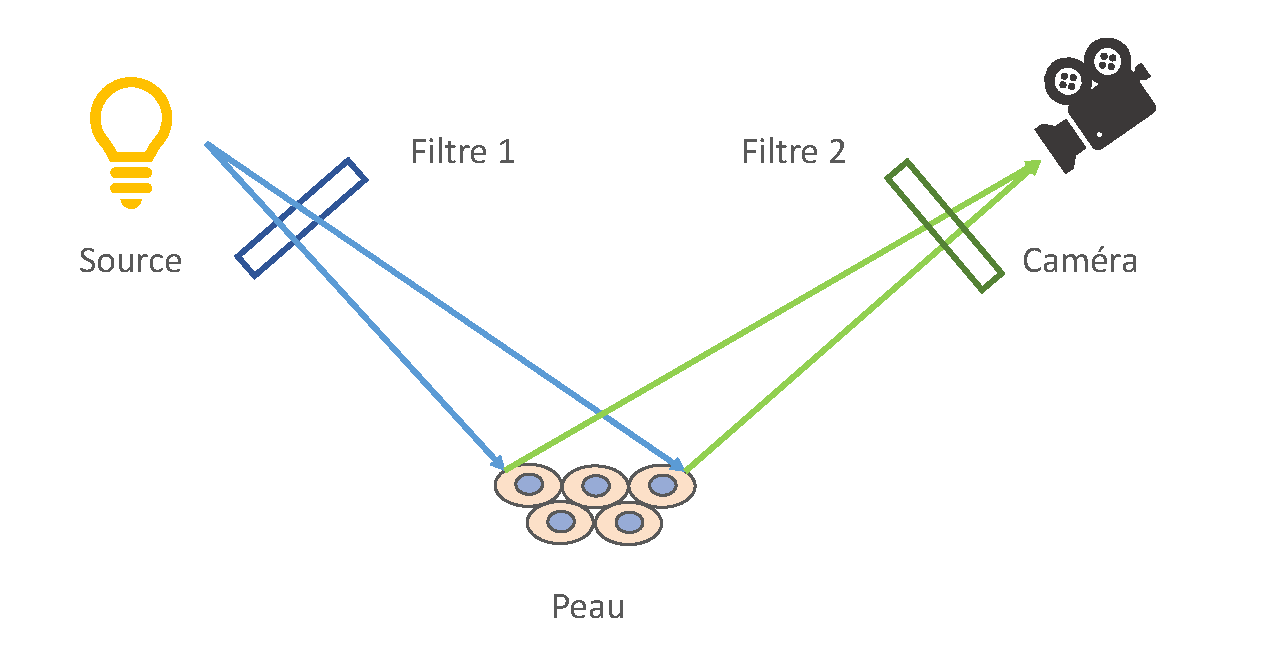
\includegraphics[width=\linewidth]{contents/chapter_2/resources/scheme_multispectral_principle.pdf}
    \caption{Schéma de fonctionnement d'une caméra multispectrale. Les dispositifs peuvent de nos jours adapter la longueur d'onde de la source à partir d'éclairage \gls{led} ou de filtres de lumière (Filtre 1), ou capter différentes longueurs d'ondes à partir de la lumière ré émise (Filtre 2).}
    \label{fig:scheme_multispectral_principle}
\end{figure}\par

\subsubsection{Microscopie confocale Raman}
Ce type de dispositif porte le nom de l'effet Raman, lui-même inspiré par le nom du physicien Chandrashekhara Venkata Râman à l'origine de cette découverte. Son principe consiste à analyser un décalage de fréquence entre la lumière incidente et la lumière diffusée. Ainsi, ce décalage est propre à chaque matériau et permet de retrouver ce dernier. Cet effet est par son principe non destructif, et a l'avantage de ne pas être dépendant de la longueur d'onde d'excitation. Contrairement à l'effet de fluorescence pour lequel la lumière doit posséder une longueur d'onde spécifique afin d'entrer en "résonance" avec la matière traversée, l'effet Raman s'obtient quelle que soit la longueur d'onde de la lumière. Les différentes interactions et leurs différences sont schématisées sur la \Cref{fig:scheme_principle_raman}.\par

\begin{figure}[H]
    \centering
    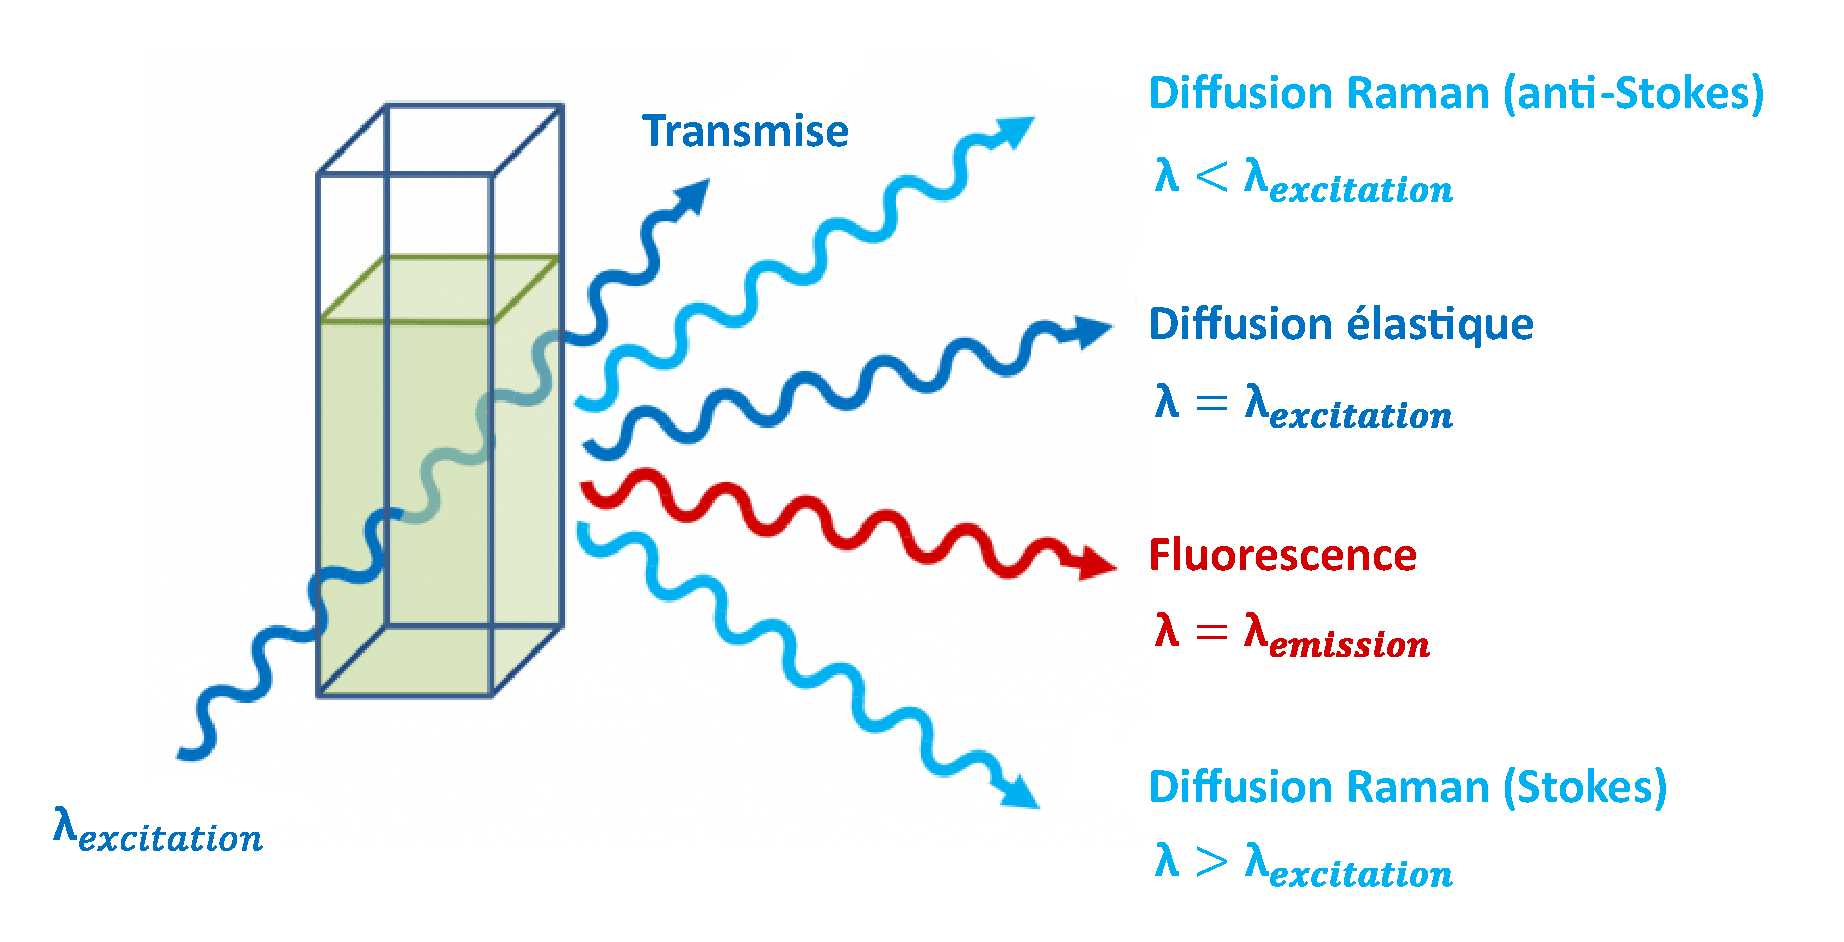
\includegraphics[width=\linewidth]{contents/chapter_2/resources/scheme_principle_raman.pdf}
    \caption{Schéma reprenant les divers effets résultant de l'interaction entre la lumière et la matière\textsuperscript{\ref{footnote:edinburgh_instruments}}. La diffusion Raman se distingue par un décalage de longueur d'onde supérieur (Stokes) ou inférieur (anti-Stokes).}
    \label{fig:scheme_principle_raman}
\end{figure}\par

\addtocounter{footnote}{1}
\footnotetext[\thefootnote]{Source~: Edinburgh Instruments, Livingston, Royaume-Uni. \label{footnote:edinburgh_instruments}}

Cet effet a été employé en spectroscopie assez tôt~\cite{Ferraro2003,Ferraro2003b} et s'est étendu progressivement à la microscopie confocale~\cite{Casper2003} permettant d'obtenir non plus une information relative à un point unique, mais d'obtenir des images à deux dimensions, avec une profondeur ajustable par modification du plan focal.\par

Ses applications dans le milieu de la dermatologie sont variées. En effet, de nombreux travaux ont porté sur la détection des lésions cancéreuses mélanocytaires, dont essentiellement le mélanome avec une sensibilité supérieur à 90\%~\cite{Lui2012,Schleusener2015}. Les lésions cancéreuses non mélanocytaires ont également été abordées dont essentiellement le \gls{bcc} et le \gls{scc} avec des précisions de détection élevées, supérieures à 90\%~\cite{Lieber2008,Silveira2015}.\par
\clearpage

\subsection{Modalités par mesure non optique}
Nous évoquons au travers de ces quelques lignes des modalités alternatives aux techniques optiques employées dans le milieu de la dermatologie à titre plus expérimental. Nous décrivons dans un premier temps le fonctionnement de l'\gls{mri} et dans un second temps celui de l'échographie haute fréquence.\par

\subsubsection{Imagerie par résonance magnétique}
Le principe global de fonctionnement de l'\gls{mri} est basé sur l'interaction et l'observation des moments magnétiques des noyaux d'hydrogène. A leur état initial, les noyaux d'hydrogène possèdent un moment magnétique non contraint et donc désordonné (la somme de ces moments magnétiques à l'échelle macroscopique est approximativement nulle). Ainsi, la première étape consiste à contraindre le moment magnétique des noyaux d'hydrogène dans une même direction (mais pas forcément un même sens) par un champ magnétique constant, on parle de précession. Dans une seconde étape, des radio-fréquences sont émises pour contraindre, de manière homogène, ces moments magnétiques dans une nouvelle direction (généralement perpendiculairement à ce champ) et ce par excitation. Enfin, l'émission de radio-fréquences est stoppée, puis le temps de retour à l'équilibre est mesuré (temps de relaxation) à l'aide d'une antenne de réception. Ce fonctionnement est résumé à l'aide du schéma disponible sur la ~\Cref{fig:scheme_principle_mri}.\par

\begin{figure}[H]
    \centering
    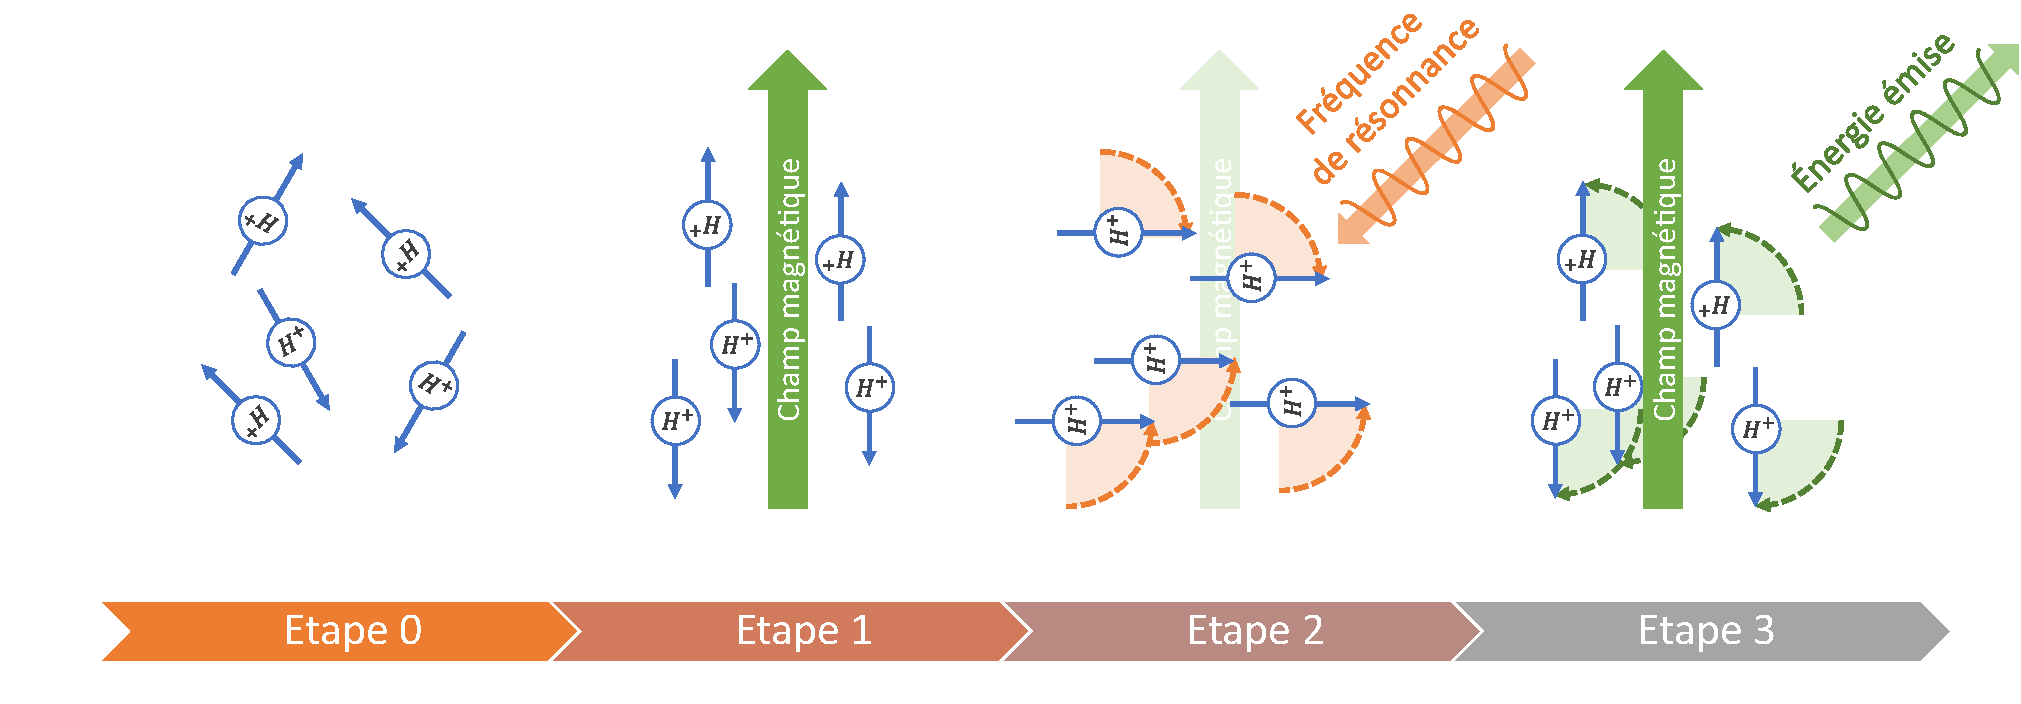
\includegraphics[width=\linewidth]{contents/chapter_2/resources/scheme_principle_mri.pdf}
    \caption{Schéma du principe de fonctionnement de l'\gls{mri} en quatre étapes. Le champ magnétique constant permet de contraindre les noyaux d'hydrogène, puis l'excitation par radio-fréquence permet d'observer par la suite leur temps de relaxation.}
    \label{fig:scheme_principle_mri}
\end{figure}\par

En ce qui concerne l'utilisation de l'\gls{mri} en dermatologie, le champ d'application semble assez restreint, malgré des études positives concernant son utilisation dans le cadre de dépistage et l'utilisation à but pré-opératoire du mélanome. De plus, l'utilisation d'agent de contraste comme le gadolinium semble être opportun pour le dépistage de lésions de la peau~\cite{Zemtsov1993}. Une étude plus récente liée à la dermatologie a été menée sur les mécanismes nerveux de récompense associés aux démangeaisons, mais impliquant une \gls{mri} fonctionnelle du cerveau et non de la peau en elle-même~\cite{Mueller2017}. Néanmoins, l'une des principales contraintes évoquée concerne l'acquisition d'échantillons de faible taille sur des machines conventionnelles rendant le ratio signal sur bruit important et les temps d'acquisition pour compenser ce dernier inexploitable~\cite{Gobel2016}. De plus, les forts coûts associés à ces appareils et leur utilisation contraignante en font des outils difficilement applicables au domaine de la dermatologie.\par

\subsubsection{Échographie haute fréquence}
Les dispositifs d'échographie sont des appareils d'imagerie basés sur l'utilisation d'ondes acoustiques. Pour cela, une sonde composée de transducteurs électro-acoustique est employée pour l'émission mais également la réception de ces ondes, par utilisation de l'effet piézoélectrique inverse et direct. Il existe de multiples sondes pouvant émettre à divers intervalles de fréquences et permettant d'atteindre diverses profondeurs. Ces ondes sont ainsi émises par la sonde (effet piézoélectrique inverse) et se propagent au sein des tissus du corps humain, avant d'être partiellement renvoyés à chaque changement de l'impédance de ces tissus. Les ondes renvoyées sont ainsi réceptionnées par la sonde émettrice (effet piézoélectrique direct) et pour former un signal.\par

Comme énoncé différentes fréquences sont employées selon la profondeur recherchée, de \SIrange{2}{10}{\mega\hertz} pour des structures assez lointaines allant de l'abdomen aux artères, et \SIrange{10}{70}{\mega\hertz} pour des structures plus proches et fines telles que la peau et l'oeil. Ainsi, les travaux de la peau par échographie emploient le terme d'échographie haute fréquence.\par

Les travaux de recherches mêlant dermatologie et échographie avant les années 2000 ont montré une efficacité de la technique afin de suivre l'évolution de mélanomes~\cite{Cammarota1998}. Des travaux plus récents ont permis d'étendre la techniques à d'autres pathologies cancéreuses tels que les \gls{bcc}~\cite{Barcaui2014}, mais également des \gls{scc}~\cite{Catalano2010}. Enfin, cette technique aurait un potentiel pour le suivi de pathologies plus bénignes tels que l'eczema ou l'arthrose psoriasique~\cite{Bhatta2018}.\par

\begin{figure}[H]
    \centering
    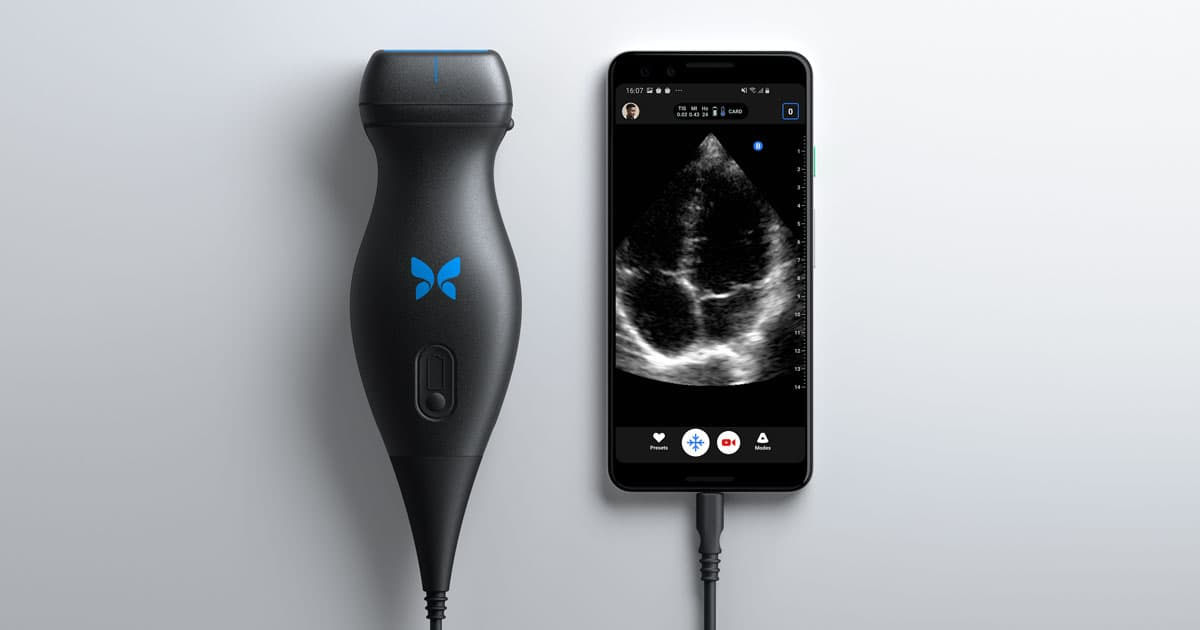
\includegraphics[width=\linewidth]{contents/chapter_2/resources/exemple_ultrasound.jpg}
    \caption{Exemple de la sonde à ultrasons Butterfly iQ\textsuperscript{\ref{footnote:device_ultrasound}}, proposant une solution nomade et connectée.}
    \label{fig:exemple_ultrasound}
\end{figure}\par


\addtocounter{footnote}{1}
\footnotetext[\thefootnote]{Source~: Butterfly Network, New York, États-Unis. \label{footnote:device_ultrasound}}
\chapter{Intelligence artificielle et notion complémentaires}
\label{chap:chapter_3}
\chapterintro
Lors du précédent chapitre, les interactions entre la peau et la lumière ont été abordées ainsi que les dispositifs majeurs permettant l'acquisition d'informations de la peau.\par

De nos jours, l’informatique est une ressource omniprésente dans de nombreux domaines d’application. Ses facultés à divertir ou encore à guider ses usagers dans leurs choix quotidiens personnels et professionnels en font un précieux allié.\par 

De nouvelles pratiques font leurs apparitions, intégrant la machine au cœur des processus décisionnels. Les disciplines médicales évoluent largement et l’ordinateur permet de répondre aux besoins croissants de précision et reproductibilité (intra et inter opérateur) et de gain de temps au sein de la pratique clinique. Il s’agit également d’un moyen de formaliser la connaissance au travers d’un outil, qui dans un cadre bien défini, peut être utilisé par des non-initiés.\par

Cette nouvelle partie permet de dérouler un peu plus le plan de ce manuscrit, en abordant cette fois-ci les systèmes d'intelligence artificielle et leur utilité vis à vis des données médicales présentes.\par
\newpage

\section{Généralités sur l'intelligence artificielle}
\label{sec:artificial_intelligence}
La notion \textbf{d’\gls{ai}} est assez souvent contestée, mais se définit plus généralement comme étant « L’ensemble de théories et de techniques mises en œuvre en vue de réaliser des machines capables de simuler l'intelligence humaine »~\textsuperscript{\ref{footnote:ia_larousse}}. Ainsi, dans cette définition, ces techniques ne se limitent pas à la reproduction du comportement interactif social humain souvent représenté dans les médias. La mise en pratique sous forme informatique de mécanismes dédiés à la prise de décision à partir de données ou encore, la retranscription du raisonnement d'un expert fait partie de cette définition.\par

Une vision plus complète de ce terme consiste a décomposer l'\gls{ai} en une discipline organisée en sous domaines possédant chacun leurs spécificités, comme schématisé sur la \Cref{fig:scheme_overview_ia}. Ainsi, le terme \textbf{d'apprentissage automatique} ou de "Machine Learning" caractérise un premier sous champ de l'\gls{ai} et est employé pour qualifier l'utilisation de mécanismes statistiques dans le but de générer des règles, à partir de données d'apprentissage. Ces données étant souvent complexes, il est souvent nécessaire de laisser l'humain intervenir pour extraire l'information pertinente à l'accomplissement de la tâche souhaitée. Enfin, le terme \textbf{d'apprentissage profond} ou de "Deep Learning" désigne un sous champ de l'apprentissage automatique, dans lequel des couches de prises de décision vont permettre d'augmenter la complexité des relations entre les données d'entrée et les tâches.\par

\addtocounter{footnote}{1}
\footnotetext[\thefootnote]{Source~: Encyclopédie Larousse. \label{footnote:ia_larousse}}

\begin{figure}[H]
    \centering
    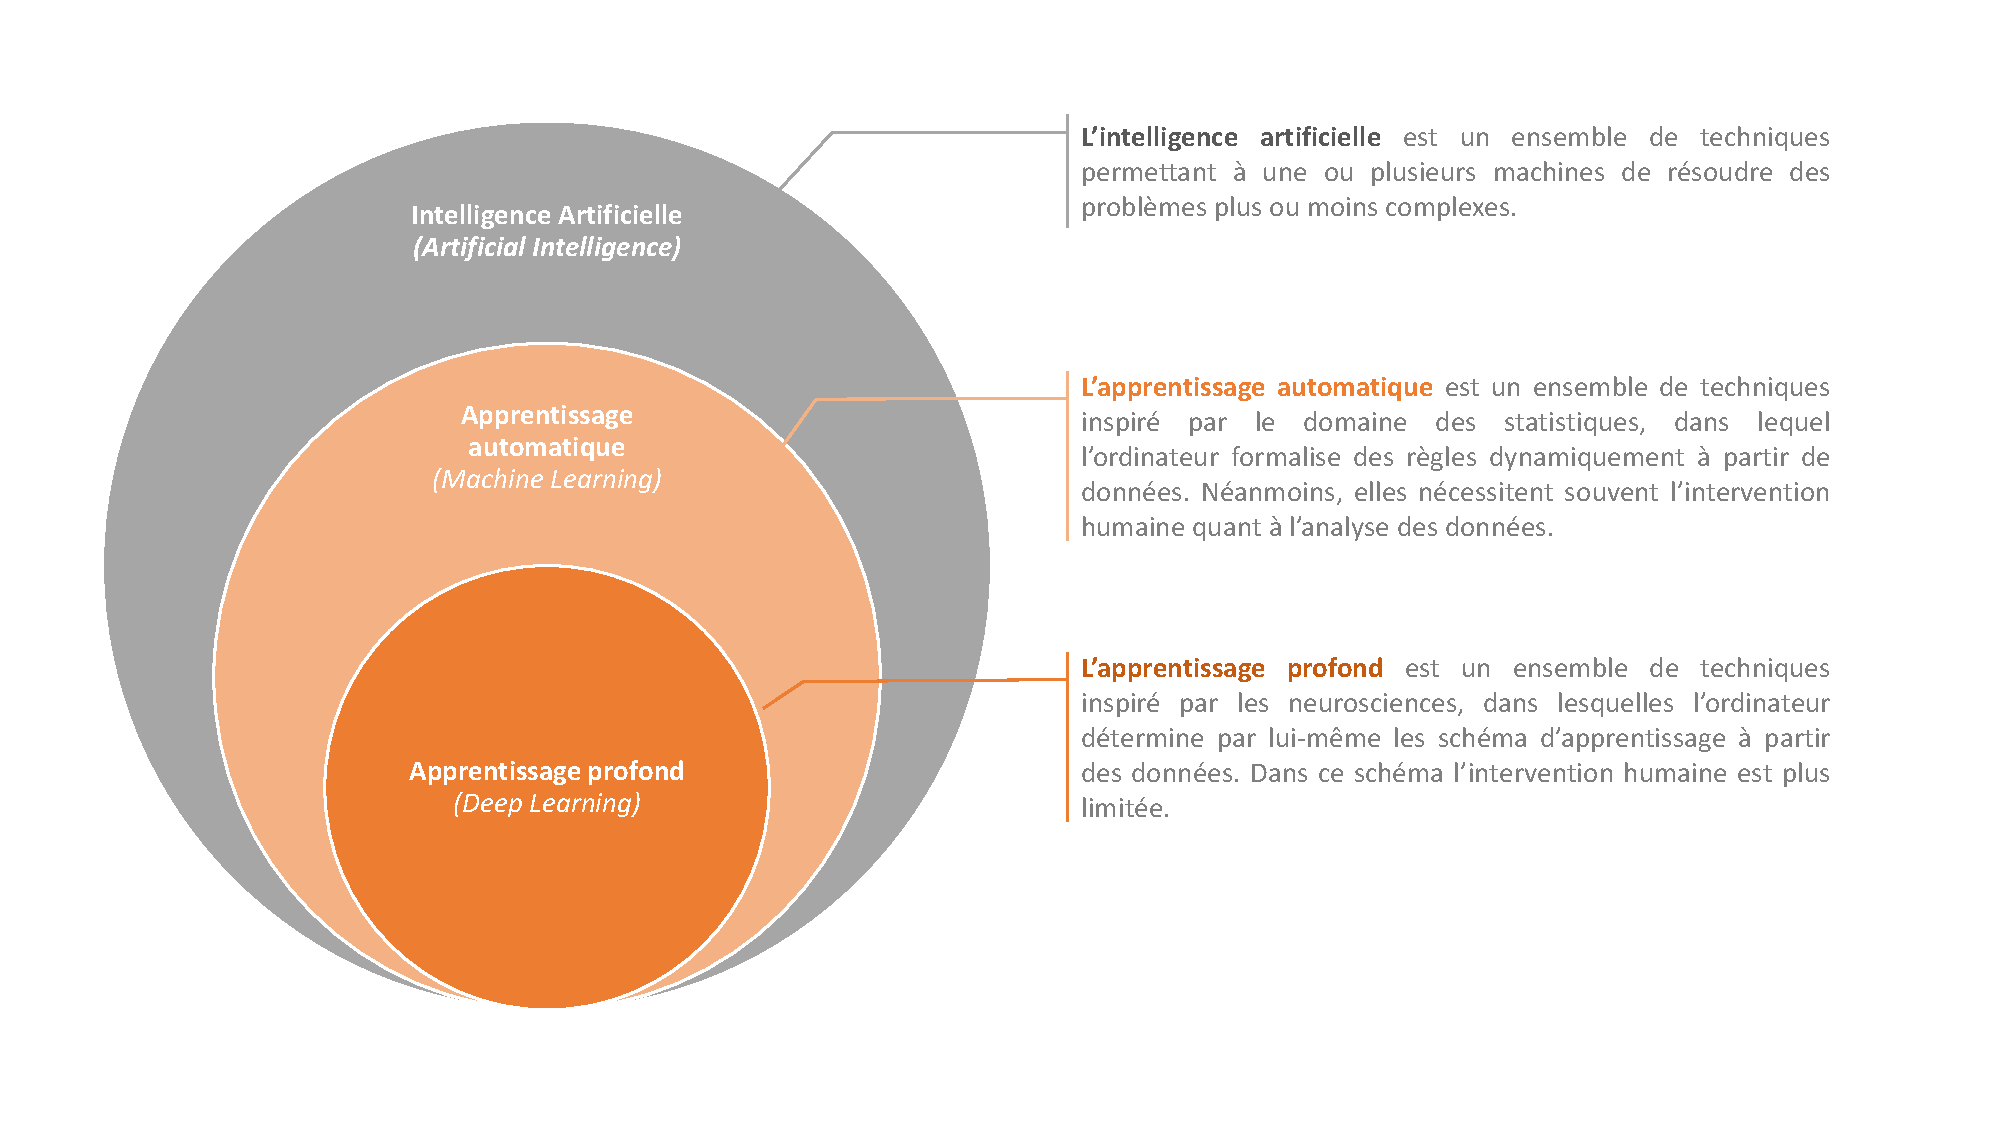
\includegraphics[width=\linewidth]{contents/chapter_3/resources/scheme_overview_ia.pdf}
    \caption{Représentation des relations entre "Intelligence artificielle", "Apprentissage automatique" et "Apprentissage profond".}
    \label{fig:scheme_overview_ia}
\end{figure}\par

Cette partie a pour vocation d’amener à la compréhension générale des courants d’\gls{ai}, qui permettent la résolution de problématiques variées telles que la dermatologie. Dans une première section, les approches par apprentissage sont décrites, puis par extension amène à la présentation de l'apprentissage profond dans une seconde section. La troisième section décrit les méthodes permettant le paramétrage et l'évaluation de ces modèles. Enfin, la dernière section décrit les principes de fusions utiles à ce travail.\par

\section{Approches par apprentissage}
\label{sec:machine_learning}
Ce courant a été « évoqué » en 1948 par Alan Turing ; son idée était de proposer des « machines à apprendre susceptibles de construire elles-mêmes leurs propres codes » \cite{Turing1950}. En 1959, Arthur Samuel formule une première définition des approches par apprentissage comme étant un « domaine d’étude dans lequel la possibilité est donné à l’ordinateur d’apprendre sans avoir été explicitement programmé ».\par 

Les approches par apprentissage automatique peuvent être résumées aux techniques permettant à un système informatique d’adapter son analyse et son comportement en fonction de ses données d’entrée. Une définition plus formelle et récente de ce domaine proposée par Tom Michael Mitchell est qu’un « programme informatique apprend d’une expérience E, en adéquation avec des tâches T et une mesure de performance P, si sa performance sur les tâches T, mesurée par P, s’améliore avec l’expérience E ».\par

Ainsi au sein des courants d’apprentissage, deux grandes sous catégories synthétisé dans la \Cref{fig:scheme_machine_learning} peuvent être distingués, dont~: 
\begin{itemize}
    \item L'apprentissage \textbf{supervisé} correspond aux techniques visant à faire correspondre les données d'entrée avec des sorties de valeurs discrètes (on parle aussi de classification) ou continues (on parle alors de régression),
    \item L'apprentissage \textbf{non-supervisé} correspond à des approches exploratoires, dans lesquelles l'ordinateur tente d'identifier des corrélations au sein des données (désigné par le terme de clustering),
    \item L'apprentissage \textbf{semi-supervisé}~\cite{Murphy2012} reprend les précédentes théories afin d'exploiter au mieux l'ensemble des données à disposition et de mieux discerner le problème.
\end{itemize}

Les prochaines sous-sections abordent chacune de ces catégories.\par
 
\begin{figure}[H]
    \centering 
    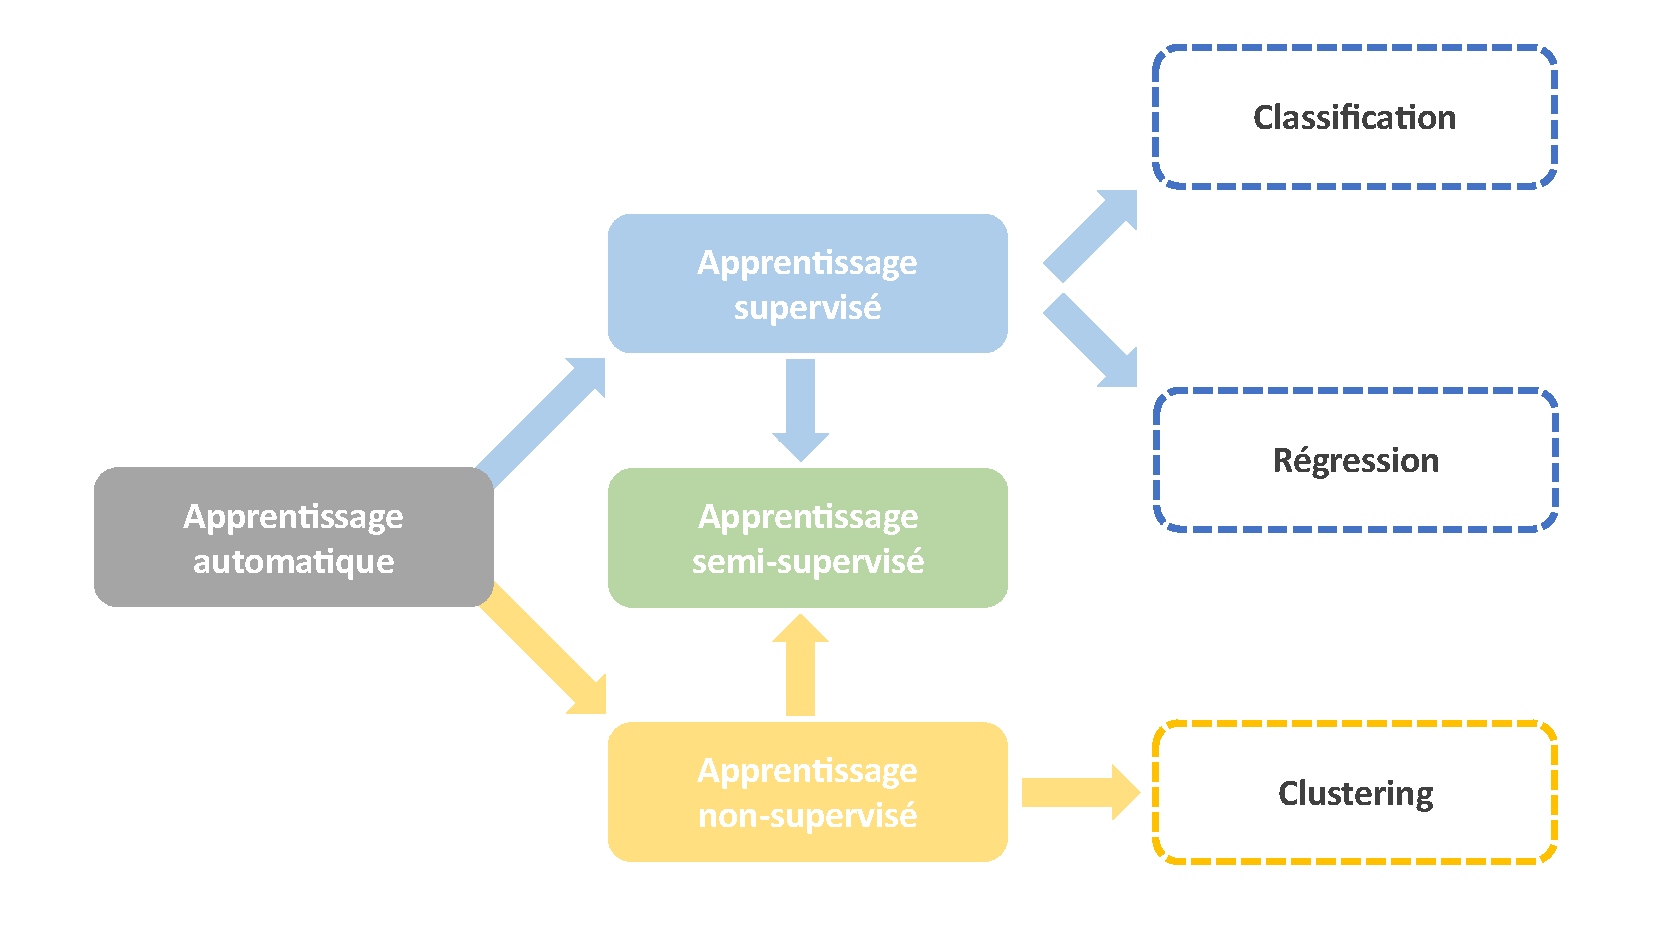
\includegraphics[width=\linewidth]{contents/chapter_3/resources/scheme_machine_learning.pdf}
    \caption{Schéma de décomposition des approches par apprentissage automatique.}
    \label{fig:scheme_machine_learning}
\end{figure}

\subsection{Apprentissage supervisé}
\label{sec:supervised_learning}
L’apprentissage supervisé consiste à déterminer la relation permettant de faire correspondre des données d’entrée $x$ et des données de sorties $y$ et cela, dans le but de produire sur de nouvelles données d’entrée $x'$, de nouvelles sorties $y'$.\par

Cette approche implique l’utilisation d’une base d’apprentissage, définie comme \textit{un ensemble de couples entrée-sortie} noté $\{(x_1,y_1 ),\ldots,(x_n,y_n )\}$ avec $n \in N$. Ainsi, l’humain tente d'apporter une signification à ces données sous forme d'annotations (ou étiquettes) pour lesquelles la machine devra être en mesure de trouver la relation existante.\par

Dans le but d'achever cette tâche, les variables propres à chaque observation sont supposées suffisamment discriminantes pour permettre l'identification des annotations. Ce problème est défini par la relation $y=f(x)$, où $f$ est notre fonction inconnue correspondant au phénomène observé, par une fonction d’approche $g$ appelée fonction de prédiction tel que $y=g(x)$, avec $x=\{x_1,x_2,\ldots,x_n\}$ un vecteur de caractéristiques possédant suffisamment d'information~\cite{foulds2010}.\par 

Cet apprentissage, schématisé sur la \Cref{fig:scheme_supervised_classification}, se découpe en deux processus distincts~:
\begin{itemize}
    \item \textbf{l’apprentissage} ou \textit{entraînement}, qui consiste à approcher la fonction $f$ par une fonction $g$ compte tenue de données étiquetées,
    \item \textbf{la prédiction} ou \textit{inférence}, qui consiste à prédire sur de nouvelles données à partir de $g$ tel que $g(x') = y'$.
\end{itemize}\par

\begin{figure}[H]
    \centering
    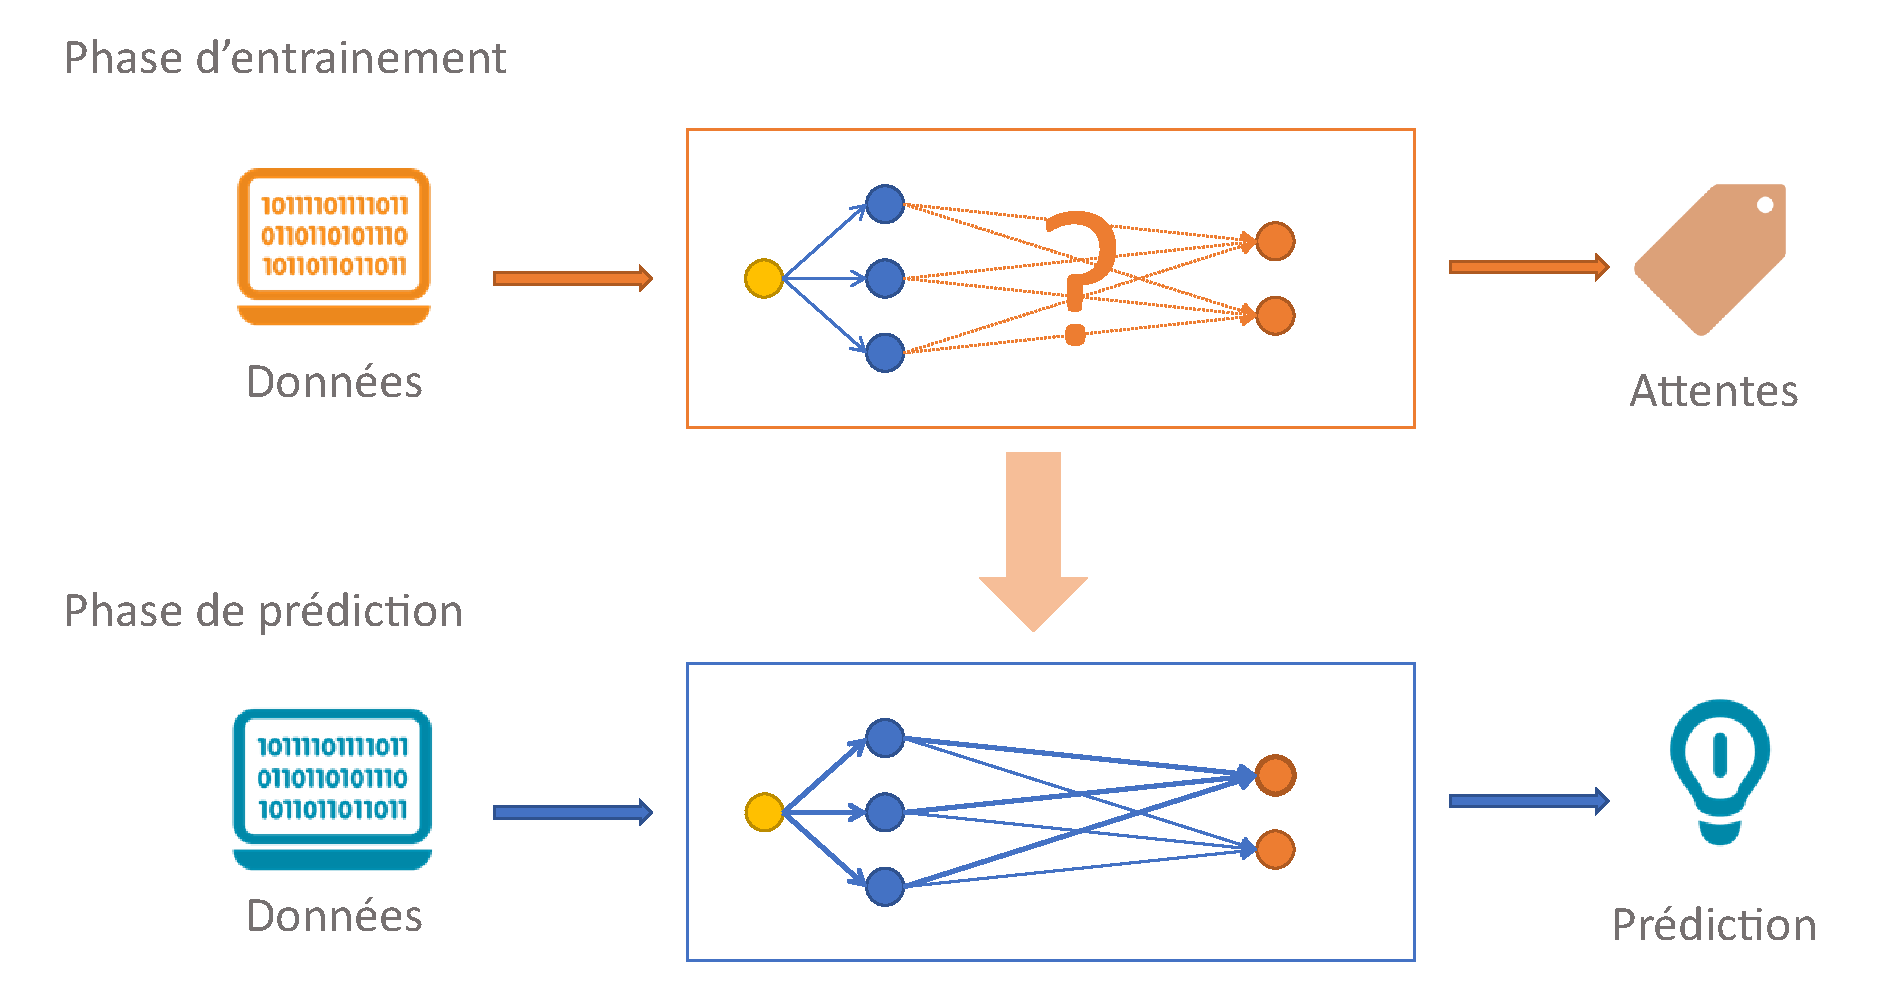
\includegraphics[width=0.8\linewidth]{contents/chapter_3/resources/scheme_supervised_classification.pdf}
    \caption{Schéma de l’approche dite supervisée. La phase d'entraînement permet de déterminer les relations entre données et attentes, sur des données connues dites d'apprentissage. La phase de prédiction réutilise les relation déterminées lors de la phase d'entraînement. }
    \label{fig:scheme_supervised_classification}
\end{figure}

Ces approches dites supervisées se regroupent ainsi au travers de deux catégories majeures~:
\begin{itemize}
    \item La \textbf{classification}, c'est à dire la prédiction de valeurs discrètes, soit l’ensemble des entiers relatifs noté $\pmb{\mathbb{Z}}$. Sont également utilisés les compléments de \textit{classification binaire} lorsque le problème formulé ne comporte que deux classes, et de \textit{classification multi-classes} lorsque la situation nécessite de prédire $N$ classes avec $N$ > 2.
    \item La \textbf{régression}, c'est à dire la prédiction de valeurs continues, soit l’ensemble des nombres réels noté $\pmb{\mathbb{R}}$.
\end{itemize}\par

Les travaux de ce manuscrit portent sur les méthodes de classification, traduit par la catégorisation de données images cliniques pathologiques selon divers niveau de dangerosité. En prenant appui sur l'un des travaux~\cite{Kotsiantis2007}, un échantillon de ces méthodes et de leur principe respectif est fourni, dont~:
\begin{itemize}
    \item \textbf{Les approches logiques} qui correspondent à des approches par succession de décisions~\cite{Kotsiantis2007}. Dans cette catégorie, nous retrouvons les arbres de décision~\cite{Breiman1984} (également connu sous le terme de \gls{cart}) dont le principe peut se résumer à la construction d'un graphe, dans lequel chaque noeud est associé à une décision caractérisée par le choix d'une caractéristique et d'un seuil~\cite{Quinlan1986}. Toute la complexité de ces approches repose sur le choix de ces caractéristiques, Ainsi, les caractéristiques sont utilisées par ordre d'importance dans la séparation du problème.
    \item \textbf{Les approches statistiques} qui correspondent à des approches probabilistes, qui déterminent dans quelle mesure un élément fait partie d'une classe. Le \gls{nbm}~\cite{Zhang2004} est un exemple typique de ce type d'approche, dans lequel chaque caractéristique est considérée comme indépendante. La relation entre caractéristique et annotation se définit ainsi comme le produit des probabilités de chacune d'entre elles d'appartenir à la classe supposée (voir l'\Cref{eq:bayesian}). Ce type de classification bayésienne peut également être étendue sous la forme de réseau~\cite{Kononenko1989}.
    \item \textbf{Les approches par instances} qui qualifient des méthodes consistant à une accumulation des échantillons afin d'enrichir un espace et non pas de leur interprétation menant à une forme de connaissances. La méthode la plus connue reposant sur ce principe est celle des \gls{knn}~\cite{Cover1967}, dont la théorie majeure repose sur l'appartenance d'une donnée à une classe si celle-ci est suffisamment proche par ses caractéristiques, d'échantillons pré-existants de cette dernière. Il est alors nécessaire de définir un critère de distance, le principal utilisé étant celui de la distance euclidienne. 
    \item \textbf{Les approches par \gls{svm}}~\cite{Cortes1995} correspondent à des approches assez récentes dont le principe se résume à déterminer une frontière de séparation entre les diverses classes, qui maximise une marge suffisante permettant entre autres une meilleure tolérance au bruit. Afin de déterminer au mieux cette frontière, divers noyaux ont été établis dont le plus simple d'entre eux est \textbf{le noyau linéaire}. Nous noterons également la présence \textbf{d'un noyau de fonction de base radiale} ou \textit{Radial Basis Function} considéré comme un \textit{approximateur universel}, si les données à disposition sont suffisantes~\cite{Wang2004}.
    \item \textbf{Les approches par ensembles} sont une catégorie qui qualifie les méthodes qui emploient un ensemble de modèles prédictifs afin de construire un unique modèle plus robuste. L'une de ces méthodes, les \gls{rf}~\cite{Breiman2001} sont une extension du principe d'arbre de décision précédemment évoqué, destiné à réduire le risque de sur-apprentissage du modèle initial. Cette méthode réalise $N$ sélections aléatoires d'observations, pour lequel $N$ arbres de décision sont générés. Afin de diversifier ces arbres, un mécanisme de tirages aléatoires de caractéristiques est également réalisé au niveau de chaque noeud de décision. Une autre de ces méthodes, l'\gls{gb} est un mode opératoire généralement constitué par des arbres de décisions. En opposition avec les \gls{rf} où chaque arbre de décision correspond à un modèle de prédiction faible, l'\gls{gb} consiste à diminuer de manière séquentielle une fonction de coût à chaque nouvel arbre généré~\cite{Friedman2001}.
\end{itemize}\par

\begin{equation} 
    \label{eq:bayesian}
    \hat{y} = \underset{k \in \{1, \ldots, K\}}{\operatorname{argmax}} \ p(C_k) \displaystyle\prod_{i=1}^n p(x_i \mid C_k)
\end{equation}

Devant ces nombreuses méthodes, il est difficile de déterminer un modèle optimal à une situation particulière, notamment dans le cadre de données à forte complexité. En effet, une évaluation de manière empirique de ces diverses méthodes reste encore la meilleure solution afin de déterminer ce modèle optimal, en contrepartie d'un temps de calcul important. Néanmoins, l'un des travaux menés sur la performance des modèles supervisés, a permis de déterminer un certain nombre de critères de comparaison entre ces diverses techniques mettant en valeur en général les avantages et inconvénients de chacune~\cite{Kotsiantis2007}.\par

Pour cela, nous avons, au sein de la \Cref{tab:model_comparison}, recensé la plupart des critères importants évoqués par ce travail de recherche. La performance de classification notamment, qui semble indéniable dans le champ que nous tentons d'évaluer avec une emphase forte en termes de performances pour les \gls{svm}. La vitesse d'apprentissage a également été précisée, bien que contraignante lors de nos essais, elle ne constitue pas un frein et reste le principal inconvénient des \gls{svm}. Enfin, ces derniers sont reconnus comme robustes face à des situations pouvant comporter des caractéristiques non pertinentes ou redondantes.\par

A la vue de ces éléments, il semble plus que nécessaire de considérer l'utilisation des \gls{svm} au sein de nos travaux. De même, il est nécessaire de considérer l'utilisation des deux méthodes d'approches par ensemble mentionnées, les \gls{rf} et l'\gls{gb}, pour lesquelles aucun travail comparatif généraliste n'a été trouvé. Néanmoins, une étude génomique semble plaider dans le sens des \gls{svm} et de l'\gls{gb}~\cite{Ogutu2011}. Pour finir, il est également nécessaire de considérer ces modèles de classification au sein de processus proposés par des travaux proches de notre thématique. Nous abordons plus en détails ces éléments dans leur partie respective.\par

\begin{table}[H]
  \small
  \centering 
    \begin{tabular}{lcccc}
        \toprule
                                                                    & \textbf{\gls{cart}}   & \textbf{\gls{nbm}}& \textbf{\gls{knn}}    & \textbf{\gls{svm}}\\
        \midrule
        \textbf{Performances de classification}                     & **                    & *                 & **                    & ****              \\
        \midrule
        \textbf{Vitesse d'apprentissage}                            & ***                   & ****              & ****                  & *                 \\
        \midrule
        \textbf{Tolérance aux caractéristiques non pertinentes}     & ***                   & **                & **                    & ****              \\
        \midrule
        \textbf{Tolérance aux caractéristiques redondantes}         & **                    & **                & **                    & ***               \\
        \bottomrule
  \end{tabular}
  \caption{Table de comparaison des méthodes d'apprentissage majeures de la littérature~\cite{Kotsiantis2007}. Ce tableau propose un système de notations allant de une (mauvaise performance) à quatre étoiles (bonne performance).}
  \label{tab:model_comparison}
\end{table}
\clearpage

\subsection{Apprentissage non-supervisé}
\label{sec:unsupervised_learning}
L’apprentissage non supervisé ou « descriptif » est une seconde approche d’apprentissage dans laquelle l’ordinateur tente de « découvrir » en autonomie, des corrélations au sein de jeux de données. Ces approches émergent de problématiques diverses, telles que~:
\begin{itemize}
    \item Réduire le coût, ou temps humain nécessaire, d’obtention de données étiquetées, c’est-à-dire pour lesquelles le couple de données d’entrée et de sortie attendue est connu.
    \item Découvrir les diverses relations pouvant exister au sein d’un amas de données. En effet, un label n’est qu’un échantillonnage de l’information primaire, et ne permet pas d’obtenir les relations pouvant régir des modèles complexes.
    \item Explorer de nouvelles relations de type « cause – effet », en réaction à la masse de données produites par les objets connectés. 
\end{itemize}\par

Plusieurs applications existent, telles que~:
\begin{itemize}
	\item Le regroupement par classes, des algorithmes comme les k-moyennes tentent de minimiser la différence d’énergie entre les points d’un même groupe.
	\item La réduction de dimensions sur des données à grande complexité, par projection de ces dernières sur des espaces à dimension réduite. On souhaite par ce procédé garder l’information essentielle au processus décisionnel.
	\item La découverte de relations au sein de l’information, et des relations les plus robustes entre variables et dépendances.
\end{itemize}\par
 
\begin{figure}[H]
    \centering
    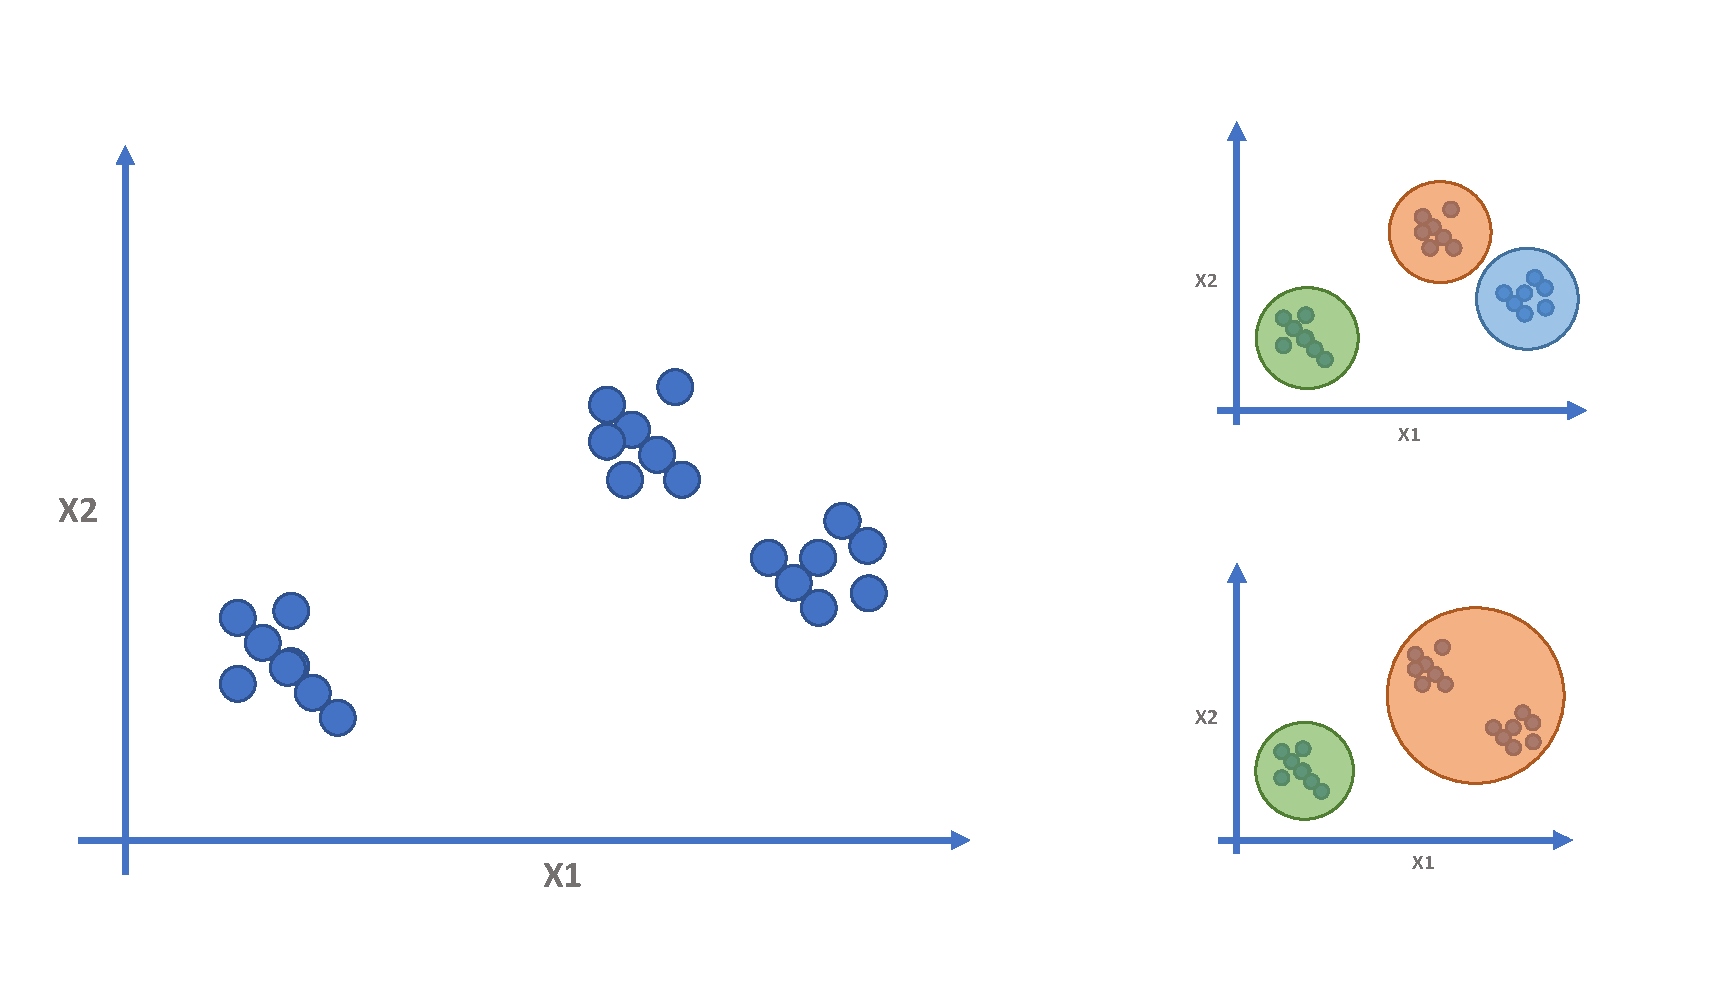
\includegraphics[width=0.8\linewidth]{contents/chapter_3/resources/scheme_unsupervised.pdf}
    \caption{Les données fournies ne sont pas associées à un label attendu. Nous demandons à la machine de découvrir des groupes de données (exemple avec 2 groupes et 3 groupes).}
    \label{fig:scheme_unsupervised}
\end{figure}

Ce principe a été également utilisé dans le but de réduire la dimension des données d'entraînement avant l'apprentissage supervisé. Cette technique porte le nom de sacs de mots ou "Bag-of-words" initialement prévue pour l'analyse de texte~\cite{Zhang2010} et utilisée dans des domaines tels que l'analyse d'image de la peau~\cite{Situ2008}.\par

\subsection{Apprentissage semi-supervisé}
\label{sec:semisupervised_learning}
Les techniques d'apprentissage semi-supervisé tentent de combiner les deux principes précédents et sont la conséquence du coût de l'annotation des données qui nécessite souvent le travail d'experts. En effet, il peut être difficile d'avoir accès à une vérité terrain qui couvre la totalité d'un jeu de données sans pour autant perdre l'apport de cette information non-annotée. Ce dernier point est particulièrement intéressant dans le cadre de données à grande dimensions pour lesquelles \textbf{l'espace} des dimensions croît de manière exponentielle et "dilue" les échantillons (connu sous le terme de "Fléau des dimensions"~\cite{Donoho2000}).\par 

Ainsi, l'apprentissage semi-supervisé se base sur plusieurs hypothèses auxquelles doivent se confronter les données~\cite{Zhu2009}, dont~:
\begin{itemize}
	\item un critère \textbf{d'homogénéité}, c'est à dire que des données issues d'une zone de haute densité partagent les mêmes annotations, 
	\item un critère \textbf{de séparation par faible densité}, c'est à dire que s'il existe une  séparation entre plusieurs types d'annotations, celle-ci se situant dans une zone à faible densité~\cite{chapelle2005}.
\end{itemize}
En pratique, il est difficile de s'assurer que les données en notre possession respectent bien ces engagements. Afin de mieux visualiser ce concept, l'exemple en \Cref{fig:example_semi_supervised} démontre l'intérêt de telles approches. Ce principe permet d'éviter d'extrapoler des frontières difficilement définissables dans une situation de faible densité de l'information étiquetée.\par
 
\begin{figure}[H]
    \centering
    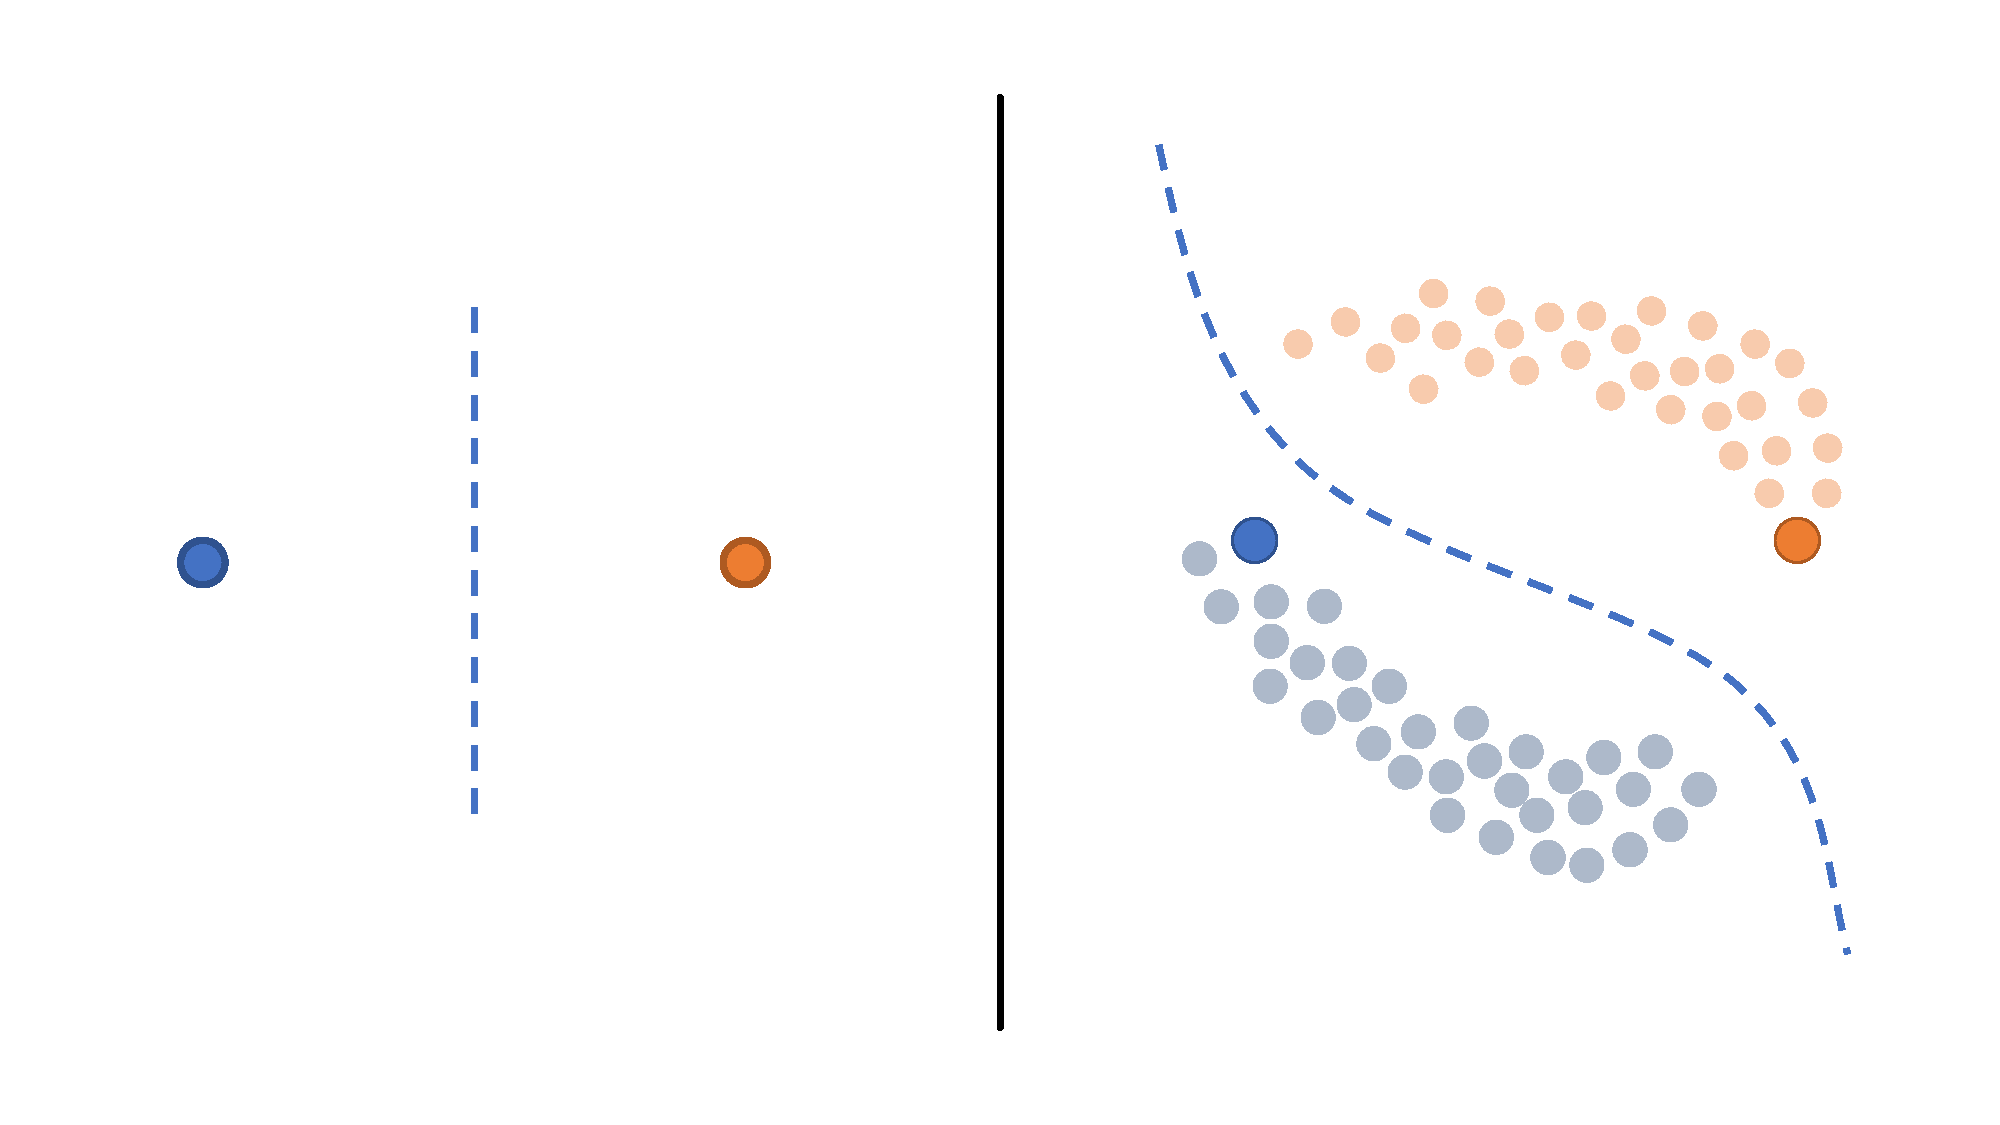
\includegraphics[width=\linewidth]{contents/chapter_3/resources/example_semi_supervised.pdf}
    \caption{Exemple fréquemment employé pour démontrer l'intérêt de l'apprentissage semi-supervisé du point de vue du principe de densité. A gauche, une classification obtenue à partir de deux données étiquetées ; A droite, la même situation avec l’ajout de données non étiquetées.}
    \label{fig:example_semi_supervised}
\end{figure}

\clearpage

\section{Apprentissage profond}
\label{sec:deep_learning}
L’apprentissage profond correspond à un sous-ensemble de l’apprentissage automatique, encouragé par les récents apports des neurosciences sur le fonctionnement et le rôle des neurones sur la prise de décisions complexes~\cite{Quartz1997,Shrager1996}. En effet, le cerveau possède divers niveaux de traitement de l’information, ce que tente d'imiter l'apprentissage profond par l'apport de multiples couches de traitement.\par

En effet, dans le cadre des méthodes « standard » d’apprentissage évoquées dans la partie précédente, la dimension de « couches » de traitement n’est pas intégrée. Les approches par apprentissage simple proposent une architecture en trois couches, dont l’une des couches est allouée à la corrélation entre les données d’entrée et de sortie. Par opposition, les approches par apprentissage profond proposant des structures en $n$ couches, avec $n \in \pmb{\mathbb{N}}$ et $n>1$. Ces couches intermédiaires sont également qualifiées de couches cachées.\par 

Nous présentons dans une première étape le principe de \gls{ann} puis dans un seconde temps le principe de \gls{cnn} et détaillons leur principe respectif. Enfin, nous abordons les aspects liés au transfert de connaissances.\par

\subsection{Réseau de neurones artificiels}
Les \gls{ann} sont des structures multicouches composées d'unités basiques appelées neurones. Dans ce schéma, chaque neurone ou unité est connecté à l'ensemble des unités de la couche $N-1$ et $N+1$ et forme un "maillage".\par

Les neurones se partagent ainsi l'information de point à point de l'entrée vers la sortie, appliquant respectivement l'opération dont ils sont responsables. Cette opération au sein d'une unité est de la forme $y = W\mathbf{x}+\mathbf{b}$ dans laquelle $W$ représente une matrice de poids qui permettra de pondérer les signaux des prédécesseurs et $b$ un terme de correction appelé biais~\cite{Stephen1990}. Ainsi, les neurones en entrée d'un réseau reçoivent une information "brute" tandis que, les neurones situés en sortie du réseau recevront une information pré-traitée par les prédécesseurs. Le schéma présent sur la \Cref{fig:scheme_deep_understanding} permet de mettre en évidence un cas simple de résolution par apprentissage pour appréhender cette notion.\par

Néanmoins, cet exemple met également en avant que ce même modèle pourrait être représenté à l'aide d'une fonction d'ordre suffisante~\cite{Bishop2006}. Ce mécanisme seul ne suffit pas à créer des réseaux exploitant les bénéfices d'un tel agencement. En effet, si une unité de ce réseau est représentée par $y = W\mathbf{x}+\mathbf{b}$, une succession de ces unités pourrait se résumer à la fonction linéaire représentée par l'\Cref{eq:proof_linearity}~\textsuperscript{\ref{footnote:equation_andrewng}}. Afin de tirer parti du potentiel de ce choix d'agencement en couches, ont été introduites des fonctions d'activation (tanh, ReLu, \ldots) qui permettent d'introduire une non-linéarité au sein de ces réseaux, permettant notamment l’autodétermination de structures de décision complexes.\par

\begin{equation} 
    \label{eq:proof_linearity}
    \begin{split}
        y = h(\mathbf{x})   &=\mathbf{b}_n+W_n(\mathbf{b}_{n-1}+W_{n-1}(\dots (\mathbf{b}_1+W_1 \mathbf{x})\dots))\\
                            &=\mathbf{b}_n+W_n\mathbf{b}_{n-1}+W_nW_{n-1}\mathbf{b}_{n-2}+\dots+W_nW_{n-1}\dots W_1\mathbf{x}\\
                            &=\mathbf{b}'+W'\mathbf{x}
    \end{split}
\end{equation}
\par

Un très bon représentant de ces types de réseaux est le \gls{mlp} utilisé à des fins de classification. Par ailleurs, un inconvénient majeur de ces réseaux est le grand nombre d'hyperparamètres à disposition. Il est ainsi délicat de procéder au choix du nombre de neurones ou même de celui des fonctions d'activation.\par

\addtocounter{footnote}{1}
\footnotetext[\thefootnote]{Source~: Plateforme de cours en ligne \href{https://www.deeplearning.ai/}{Deep Learning AI}, démonstration par Andrew Ng. \label{footnote:equation_andrewng}}

\begin{figure}[H]
    \centering
    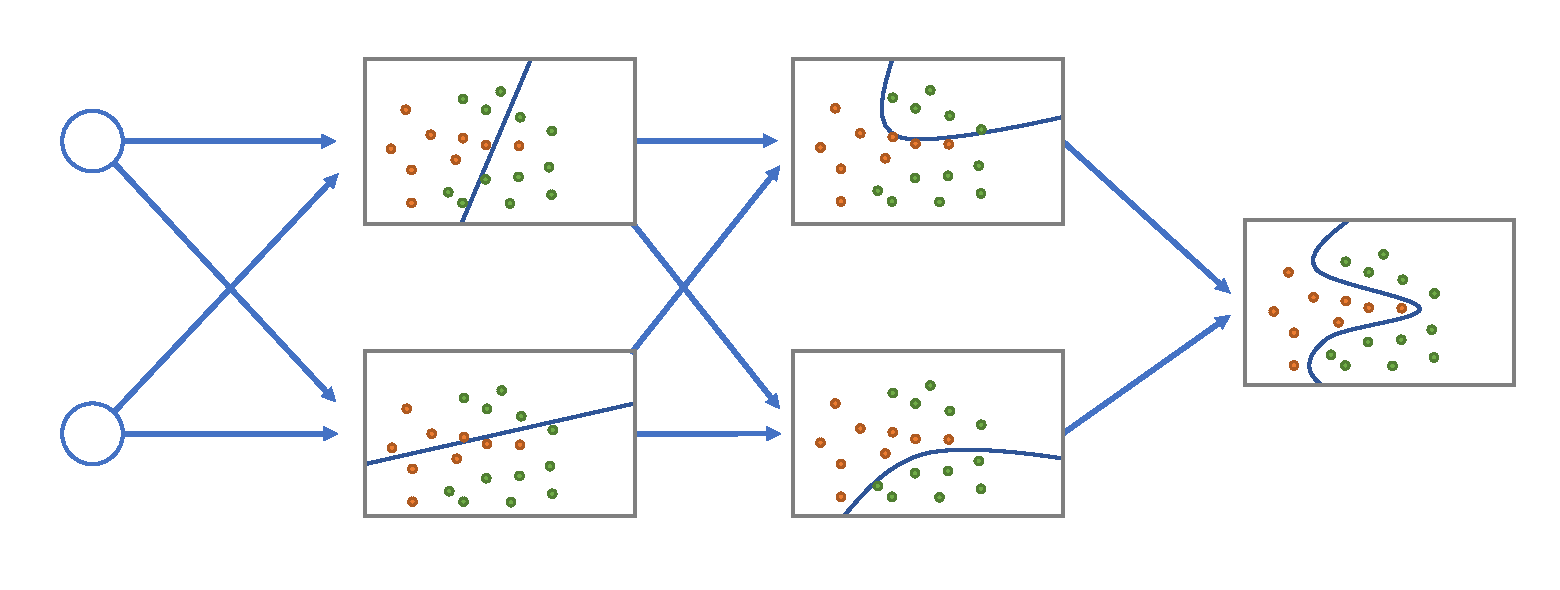
\includegraphics[width=\linewidth]{contents/chapter_3/resources/scheme_deep_understanding.pdf}
    \caption{Exemple simplifié d'une structure d’apprentissage profond. Ce modèle se compose de deux couches intermédiaires cachées~: la première couche extrait des caractéristiques linéaires simples, tandis que la seconde couche par combinaison avec la première couche conduit à une extraction de caractéristiques plus complexes. Ainsi, la première couche s'apparente à un polynôme de degré 1, tandis que la seconde couche représente des fonctions de degré 2 et ainsi de suite.}
    \label{fig:scheme_deep_understanding}
\end{figure}

\subsection{Réseau neuronal convolutif}
\label{sec:convolutionnal_neural_network}
Les \gls{cnn} sont une extension des réseaux de neurones profond, essentiellement utilisé dans un but de traitement de l'image, même si d'autres applications de ce principe peuvent être réalisées, appliquée à un signal ou à un volume par exemple.\par

Ces \gls{cnn} sont une réponse à l'application des \gls{ann} à des problématiques impliquant des données images et des contraintes multiples qu'ils comportent. Parmi ces contraintes de l'application des \gls{ann} aux images, nous pouvons évoquer~: 
\begin{inlinerate}
\item les \textbf{nombreuses connexions et paramètres requis},
\item l'\textbf{absence d'utilisation de la cohérence de l'information spatiale},
\item et la \textbf{dépendance} du réseau à la taille des informations d'entrée.
\end{inlinerate}\par

Ainsi, ces réseaux font appel à des couches de convolution permettant de résoudre ces trois principales contraintes. D'une part la convolution permet de réduire fortement le nombre de paramètres d'entraînement, le réseau n'est ainsi plus entièrement "connecté". Certaines optimisations récentes consistent à remplacer les filtres de convolution 2D par une succession de filtres 1D horizontaux et verticaux, proposant des résultats semblables et réduisant fortement le nombre de paramètres. D'autres part, la convolution permet d'apporter une logique à la dimension spatiale des données ainsi qu'une indépendance à la taille. En effet, le réseau n'est plus entièrement connecté et donc ne dépend plus d'une taille fixe, et peut ainsi traiter des données de tailles différentes mais qui doivent respecter une taille minimum. Le traitement des données par ces couches de convolution porte le nom de carte d'activation, maximum quand le produit de convolution est en phase.\par

% \begin{equation} 
%     \label{eq:convolution_integral}
%     \begin{split}
%         (f\ast g) (x) = \int_{-\infty}^{+\infty} f(x-t)g(t) \, \mathrm dt = \int_{-\infty}^{+\infty} f(t)g(x-t) \, \mathrm dt
%     \end{split}
% \end{equation}

\clearpage

\subsection{Transfert de connaissances}
\label{sec:transfer_learning}
L’apprentissage par transfert est une technique connexe à l’apprentissage profond défini comme « faisant référence à la situation où ce qui a été appris dans un contexte \ldots est exploité pour améliorer la généralisation dans une autre contexte » \cite{Ngiam2011}. Cette discipline s’inscrit dans le champ de « l’adaptation de domaine », définie comme le transfert des connaissances d’un domaine $D_S$, défini par l’hypothèse $h: X_S \rightarrow Y_S$, vers un domaine cible $D_T$ afin de satisfaire $h: X_T \rightarrow Y_T$. Son champ d'application n'est pas limité aux réseaux d'apprentissage profond, mais les contraintes qui leur sont associées font de ces techniques une ressources utile.\par

En effet, ces solutions permettent de réduire les difficultés liées à la grande quantité de ressources de calcul, de temps, mais également de données mobilisées nécessaires à un entraînement depuis sa base. Le modèle d’apprentissage attendu est alors initialement plus performant, croît plus efficacement et est plus performant qu’un apprentissage spécifique (\Cref{fig:learning_curves}).\par

Néanmoins, cette solution n’est envisageable que lorsque l’apprentissage, réalisé lors de la première tâche, généralise suffisamment le phénomène observé. Ainsi, il est d’usage courant de ne spécifier lors du transfert que la couche finale de classification du réseau, les premières couches étant employées comme extracteur général de caractéristiques. Toutefois, certaines méthodes de la littérature s’accordent sur l'entraînement conjoint des couches de classification ainsi que des couches de convolutions hautes, considérées comme moins génériques.\par

\begin{figure}[H]
    \centering
    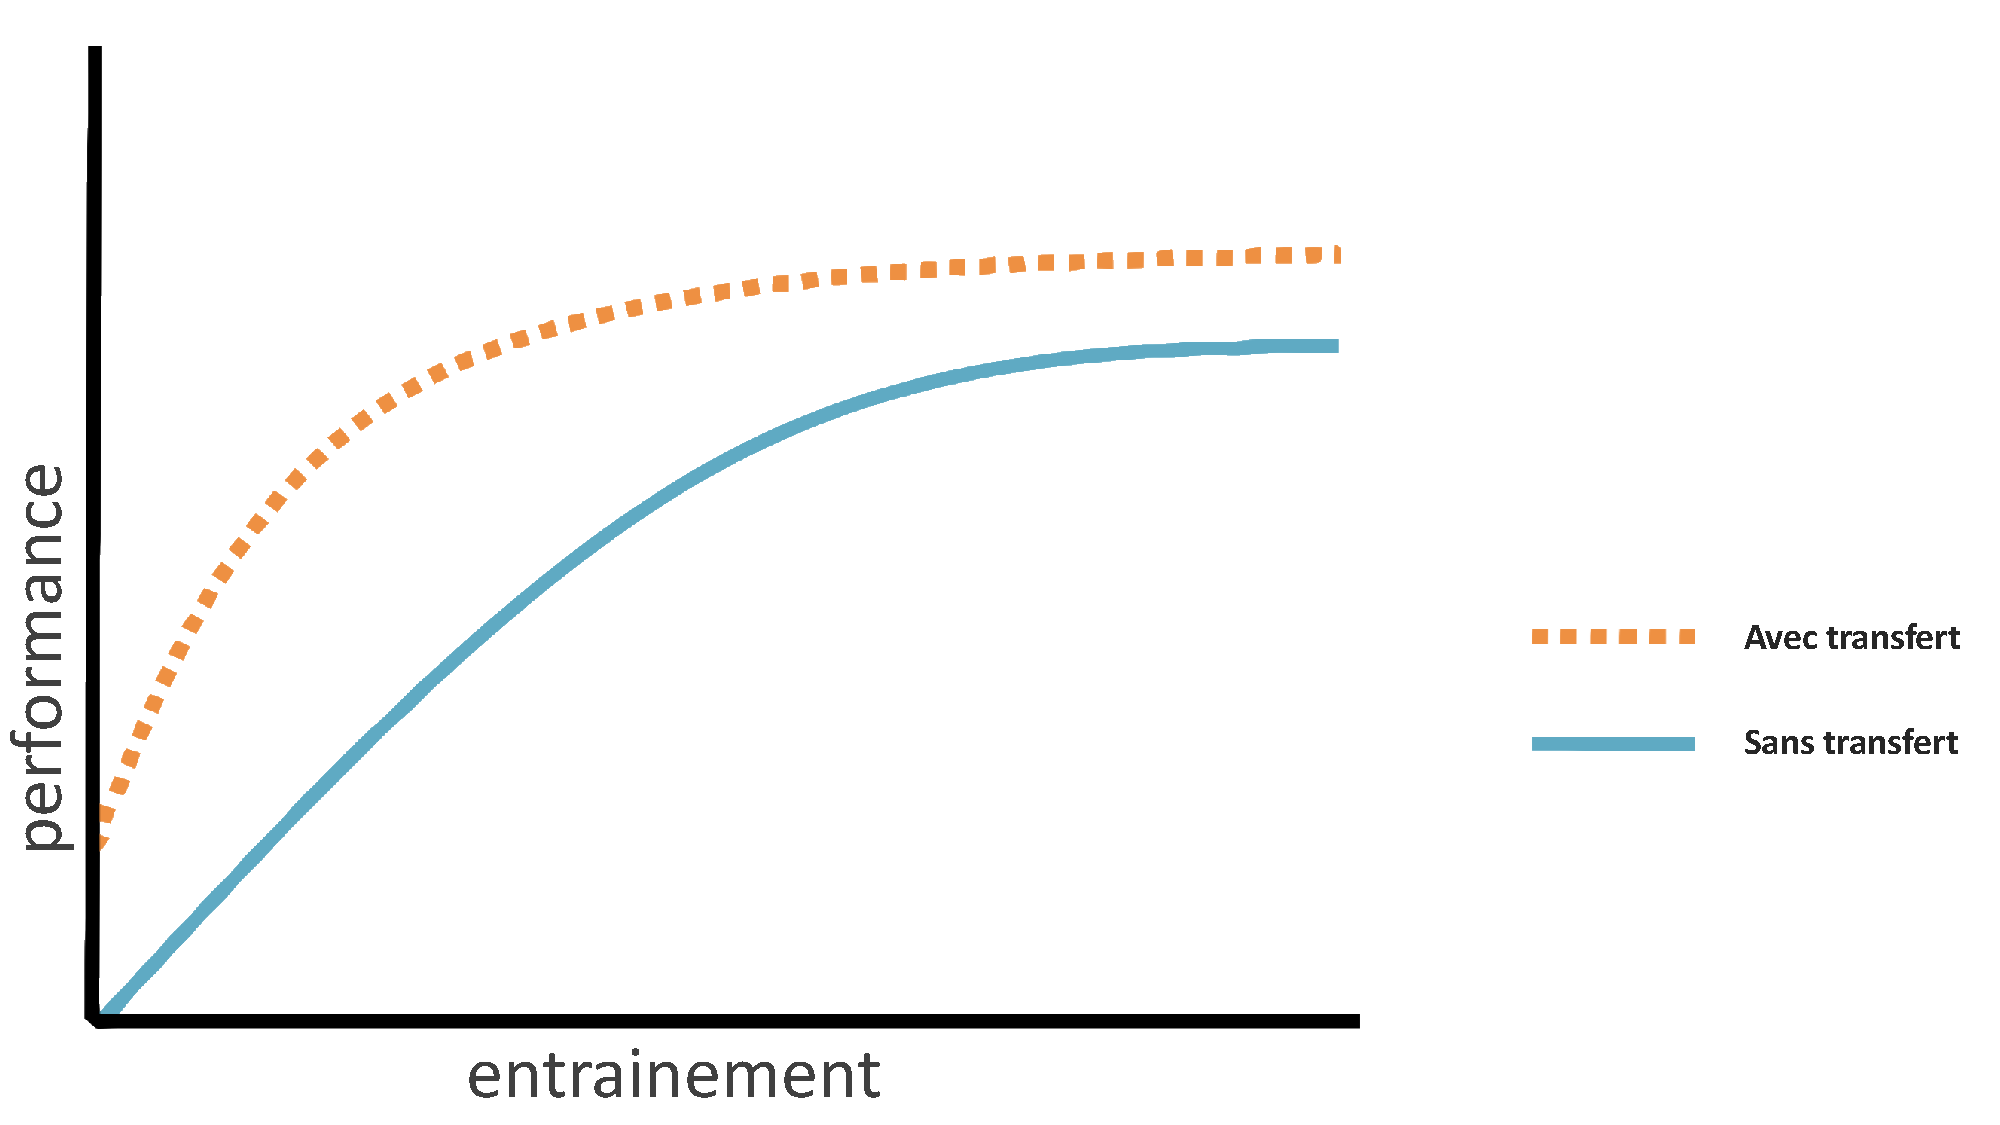
\includegraphics[width=\linewidth]{contents/chapter_3/resources/example_learning_curves.pdf}
    \caption{Exemple d'attentes liées à un apprentissage par transfert en opposition à un apprentissage classique.}
    \label{fig:learning_curves}
\end{figure}

\clearpage

\section{Paramétrage et évaluation de modèles prédictifs}
\label{sec:models_settings}
Cette partie se concentre sur des problématiques de biais lors de l'apprentissage et de l'évaluation de modèles. Nous tentons de présenter rapidement le phénomène et les risques associés, puis nous proposons des solutions permettant de s'affranchir de ces biais durant l'évaluation des modèles.\par

\subsection{Généralisation de modèles}
\label{subsec:generalized_models}
A l'aide de couples d'entrée/sortie à notre disposition, ces modèles d’apprendre une relation capable de \textbf{généraliser} et d’estimer de nouvelles sorties sur de nouvelles données. Il est pour cela nécessaire de parvenir à isoler l'information responsable de ce cheminement, plus ou moins séparable, en cause souvent la qualité de~:
\begin{inlinerate}
    \item l'hypothèse formulée, c'est à dire si la relation qui lie l'observation et sa conséquence est directe et vraie dans toute circonstance,
    \item l'information possédée, c'est à dire si l'information est juste pour répondre à la problématique cible (qualité de l'observation, rapport signal sur bruit, etc.),
    \item \ldots.
\end{inlinerate}\par 

Ce problème, évoqué dans la littérature porte le nom de « dilemme biais / variance », dans lequel le biais représente le manque de relation pertinente entre données d’entrée et de sortie et où la variance représente l’influence du modèle au petites fluctuations souvent issues de bruit. Ces termes sont intrinsèquement liés aux problématiques respectives de \textbf{sous-apprentissage} et \textbf{sur-apprentissage}. La \Cref{fig:example_underfit_overfit} reprend de manière visuelle ces problématiques, et les exprime selon un jeu d’entraînement et de test. A noter que le sur-apprentissage peut être limité par l’utilisation de termes de régularisation, de schémas de validation de modèle adaptés ou l’utilisation d’ensembles de données suffisantes.\par
 
\begin{figure}[H]
    \centering
    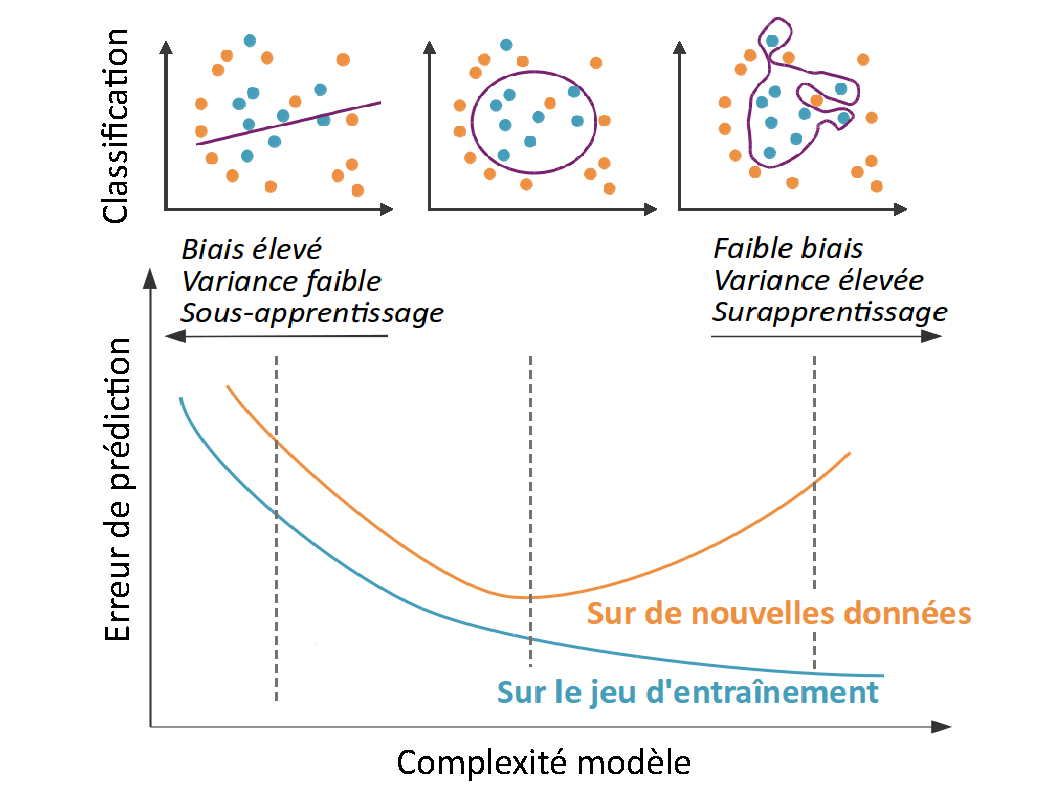
\includegraphics[width=0.8\linewidth]{contents/chapter_3/resources/example_underfit_overfit.pdf}
    \caption{Exemple de dilemme Biais/Variance. A gauche, un cas de sous-apprentissage, ce modèle est une sous approximation du phénomène observé. A droite, un cas de sur-apprentissage, le modèle ne généralise pas suffisamment le phénomène observé.}
    \label{fig:example_underfit_overfit}
\end{figure}

\subsection{Choix de métriques}
\label{subsec:metrics}
Le choix des métriques représente une part importante de nos problématiques lors de la mise en place de modèles d’apprentissage. En effet, il permet d'une part de déterminer la sélection d'un modèle parmi un ensemble de modèles et, d'autre part, de retenir des performances attendues de ce dernier par exemple dans le monde réel.\par

L’un des principaux outils à disposition afin d'évaluer la performance est la matrice de confusion, schématisé sur la \Cref{fig:scheme_confusion_matrix}. Elle permet de faire correspondre les classes réelles et prédites~: la diagonale de cette matrice fait figurer les prédictions correctement réalisées par notre modèle, tandis que les éléments restants nous renseignent sur les prédictions erronées. Dans une situation à deux classes ou \textit{binaire}, cette matrice fait ainsi ressortir quatre valeurs~:
\begin{itemize}
	\item Les \textbf{vrais positifs}, les éléments de la classe positive détectés comme positif,
	\item Les \textbf{vrais négatifs}, les éléments de la classe négative détectés comme négatif,
	\item Les \textbf{faux positifs}, les éléments de la classe négative détectés comme positifs,
	\item Les \textbf{faux négatifs}, les éléments de la classe positive détectés comme négatifs.
\end{itemize}\par

\begin{figure}[H]
    \centering
    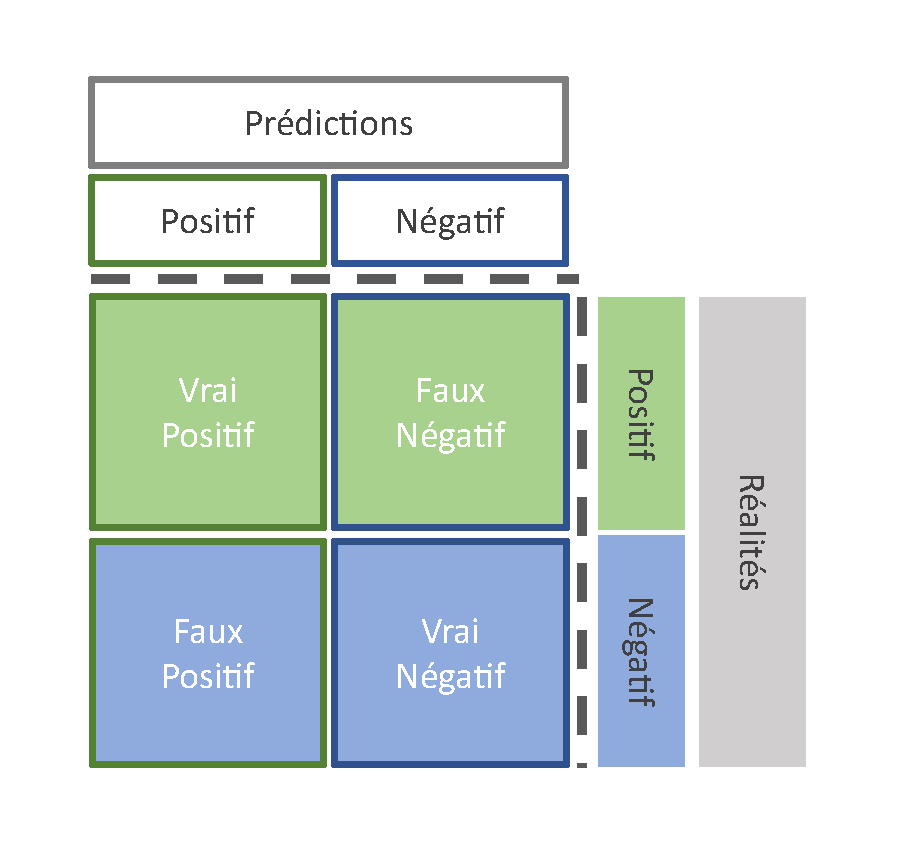
\includegraphics[width=0.55\linewidth]{contents/chapter_3/resources/scheme_confusion_matrix.pdf}
    \caption{Schéma représentatif d’une matrice de confusion, qui met en avant une situation binaire.}
    \label{fig:scheme_confusion_matrix}
\end{figure}

Bien que déjà réduite, l'information de cette matrice est encore très riche et difficile à utiliser comme critère de sélection. Pour cela, diverses métriques éprouvées sont à envisager selon la problématique à laquelle nous tentons de répondre. Parmi les plus courantes d'entre elles, les critères de précision, sensibilité ou encore spécificité sont pléthores dans la littérature mais ont tendance à ne capter qu'une partie du problème. Par exemple, la sensibilité est un critère très important en médecine ou détection de fraude, mais ne qualifie en rien la spécificité du modèle. De même, la moyenne fait également partie des critères extraits dans le domaine de l'intelligence artificielle, mais peut également manquer de sens en cas de non balancement de l'information~\cite{Guo2008} ou même ne pas mettre en avant un important gouffre entre spécificité et sensibilité. Ces métriques sont détaillés dans l'\Cref{eq:metrics_basics}.\par

\begin{equation} 
    \label{eq:metrics_basics}
    \begin{split}
    Sensibilit\acute{e} &= VP/(VP+FN) \\
    Rappel &= VP/(VP+FN) \\	
    Sp\acute{e}cificit\acute{e} &=  VN/(VN+FP) \\
    Pr\acute{e}cision &= VP/(VP+FP) \\
    Moyenne &= (VP+VN)/(VP+VN+FP+FN)
    \end{split}
\end{equation}

Dans ce cas, il peut être préférable de privilégier des métriques plus robustes, dans le cadre de données non balancées. La plupart des méthodes s’accordent sur l’utilisation de métriques tels que le \fscore{}, associant conjointement sensibilité et précision, par principe de la moyenne harmonique~\cite{Guo2008}. L'\Cref{eq:metrics_fscore} met à disposition l'expression générique de cette métrique, dont le paramètre $\beta$ permet de moduler l'importance de la précision ou du rappel. L'influence de ce paramètre est neutre lorsque sa valeur est égale à 1 comme dans le cas du \fscore.\par
 
\begin{equation} 
    {F_\beta \: score}=(1+\beta^2)*(Pr\acute{e}cision*Rappel)/((\beta^2*Pr\acute{e}cision)+Rappel)
    \label{eq:metrics_fscore}
\end{equation}
 
Une autre métrique permettant de se prémunir de ces effets de non balancement de l'information et celui de l'\acs{auc} et découlant de la courbe \gls{roc} dont le principe est résumé sur le schéma \Cref{fig:scheme_roc_curve}). La courbe \gls{roc} est tracée à partir des informations de spécificité / sensibilité et par variation d'une valeur seuil appliquée au modèle de prédiction, tandis que l'\gls{auc} correspond à l'intégration de l'aire de cette courbe. Ainsi, l'\gls{auc} est robuste au non-balancement de données mais ses valeurs sont optimistes sur des modèles de prédiction dont la variation du seuil est homogène vis à vis des résultats.\par

\begin{figure}[H]
    \centering
    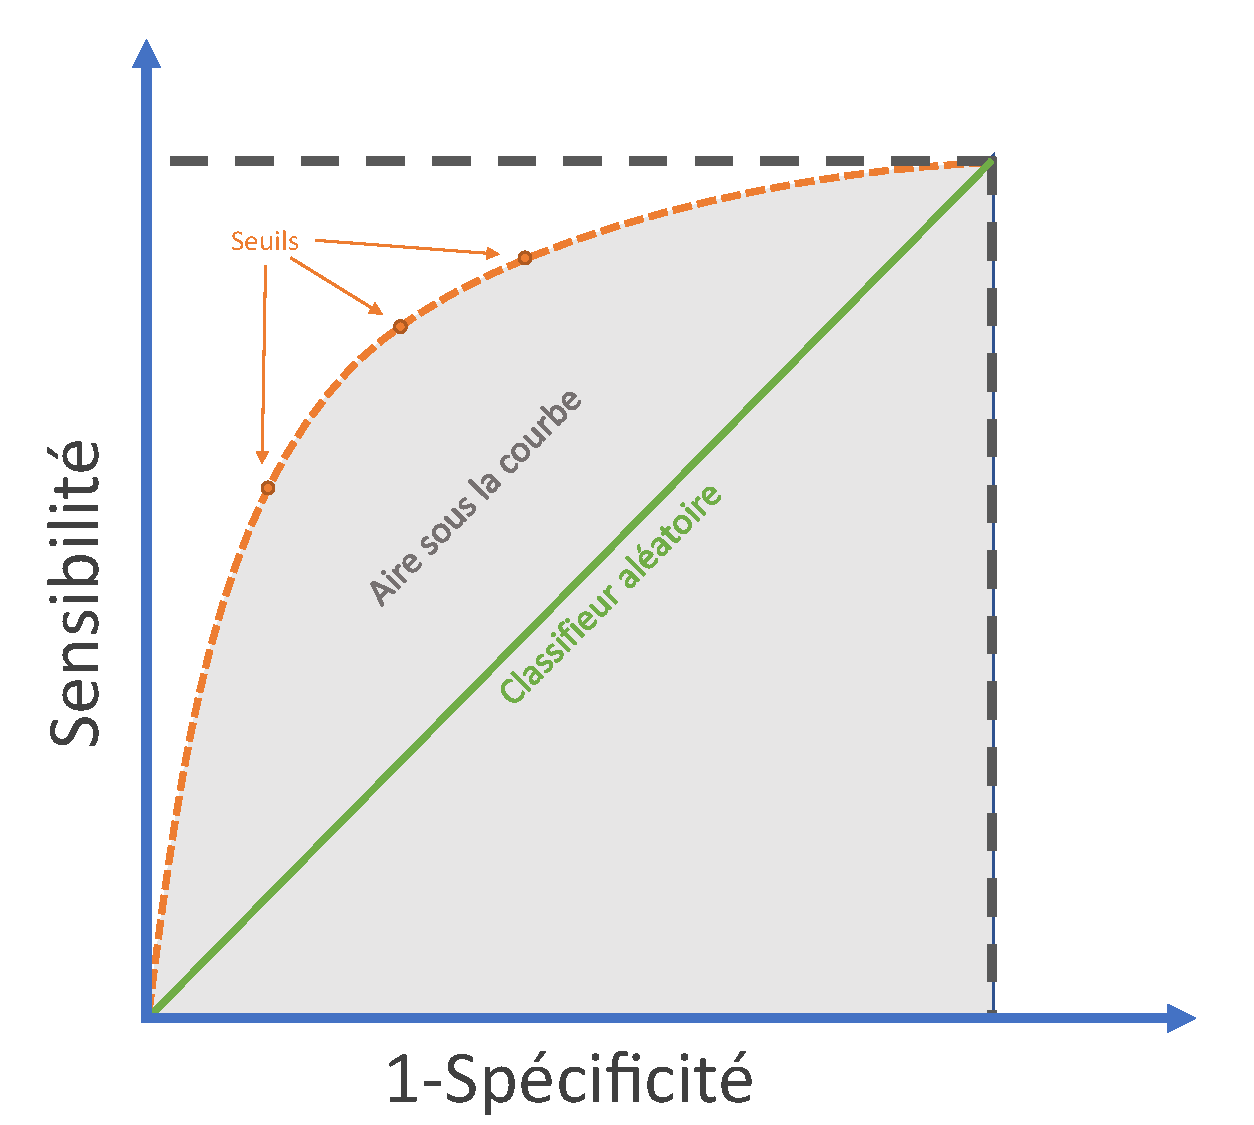
\includegraphics[width=0.55\linewidth]{contents/chapter_3/resources/scheme_roc_curve.pdf}
    \caption{Schéma de courbe \gls{roc} en orange et \gls{auc} en gris.}
    \label{fig:scheme_roc_curve}
\end{figure}

D'autres alternatives moins biaisées ont également été formulées~\cite{Sokolova2006}. Néanmoins le \fscore{} et l'\gls{auc} sont couramment utilisés dans des articles cliniques et constituent une des bases de notre travail.\par

\subsection{Réglages des hyperparamètres}
\label{subsec:hyperparameter}
Avant d’entrer plus en profondeur dans le sujet, il est nécessaire de revenir sur le terme « d’hyperparamètres ». Il caractérise les paramètres d'un processus d'apprentissage automatique dont le réglage doit être effectué avant la phase d'entraînement et dont les valeurs dépendent des données à traiter. Le réglage des hyperparamètres peut rarement être déterminé par la simple observation des données, et nécessite ainsi un réglage en fonction de chaque situation rencontrée.\par

L’une des premières techniques permettant ce réglage consiste à définir une « grille » de ces hyperparamètres, contenant pour chacun leurs possibles variations~\cite{Liu2006}. Il s'agit de la méthode la plus équitable puisqu'elle consiste à évaluer chaque combinaison par comparaison des performances finales (voir la \Cref{fig:example_hyperparameter_selection} - Gauche). Néanmoins, elle possède deux limitations majeures, dont~:
\begin{itemize}
    \item Son \textbf{temps de calcul}, qui va croître de manière exponentielle en fonction du nombre d'hyperparamètres à valider,
    \item Sa \textbf{précision}, qui va dépendre du pas choisi pour chacun des paramètres.
\end{itemize}\par

La seconde technique consiste à définir un « espace » de recherche dont la distribution de chaque hyperparamètre sera choisie, ainsi qu'un nombre d'évaluations à réaliser pour déterminer la meilleure combinaison possible. Ce nombre d'évaluation est ensuite réalisé sous forme de tirage aléatoire, effectué à l'intérieur de cet espace de recherche défini~\cite{bergstra2012} (voir la \Cref{fig:example_hyperparameter_selection} - Droite). Cette méthode possède l'avantage d'être prévisible en termes de temps puisque le nombre de combinaisons évaluées est défini au préalable et quel que soit les proportions de l'espace. Néanmoins, cette méthode possède également des inconvénients comme la représentation des tirages au sein de l'espace défini.

\begin{figure}[H]
    \centering
    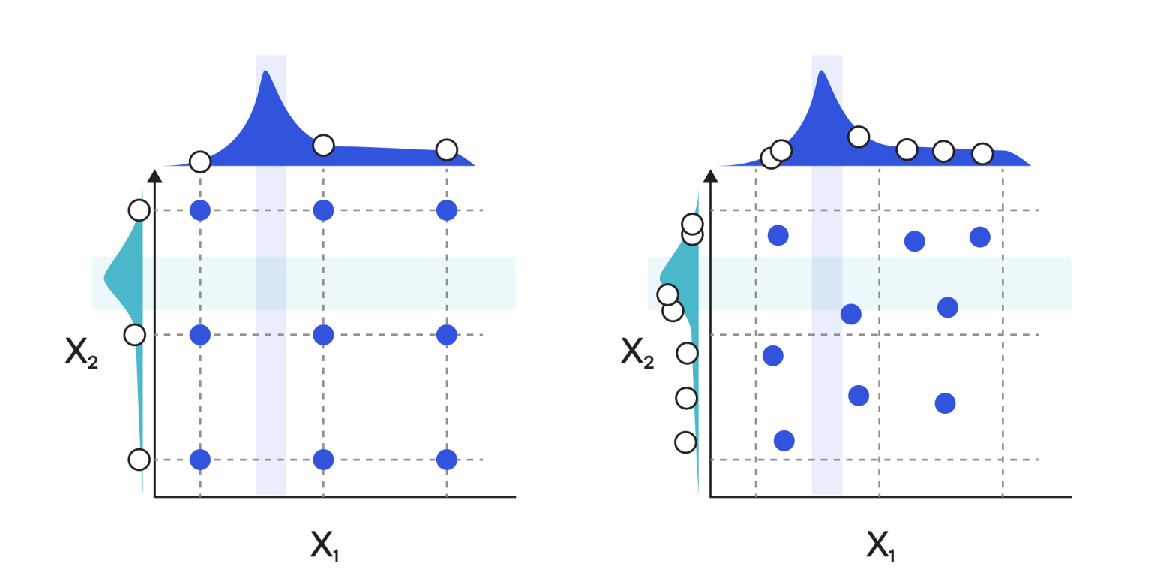
\includegraphics[width=\linewidth]{contents/chapter_3/resources/example_hyperparameter_selection.pdf}
    \caption{Exemple de recherche sur deux hyperparamètres $X_1$ et $X_2$. A gauche, une recherche sous forme de grille rigide, dans laquelle chaque combinaison est évaluée. A droite, une recherche aléatoire de ces hyperparamètres.}
    \label{fig:example_hyperparameter_selection}
\end{figure}

\subsection{Méthodes d'évaluation}
Nous avons évoqué divers éléments permettant l'ajustement des modèles, voir la \Cref{subsec:hyperparameter}, et la mesure de performance, voir la \Cref{subsec:metrics}. Il est nécessaire d'orchestrer cet ensemble afin d'obtenir la meilleure attente possible d'un modèle de prédiction, tout en conservant une mesure permettant de nous renseigner sur la fiabilité de ce modèle et de ses prédictions futures dans des situations où la vérité terrain n'est pas connue. En effet, l'évaluation d'un modèle de prédiction sur des données identiques à celles utilisées constitue un biais, par l'utilisation de connaissance \textit{a posteriori}. De même, l'ajustement des hyperparamètres rentre dans cette catégorie de l'entraînement, et l'évaluation ne peut se faire sur des données ayant servi à les déterminer. Par ailleurs, une telle évaluation permet de détecter les problèmes de sous-apprentissage et sur-apprentissage évoqués en \Cref{subsec:generalized_models}.\par

La méthode \textbf{holdout} est la plus simple d'entre elles et consiste à diviser l’échantillon de données en deux sous-ensembles respectivement d'entraînement et de test. Il est important lors de cette étape de vérifier que les données présentes dans chacun de ces sous-ensembles soient représentatives de chaque classe présente dans la problématique. Les données spécifiées pour le test restent ainsi non utilisées jusqu'à leur confrontation au modèle définitif qui est alors évalué sur ces dernières. Le principal inconvénient de cette méthode est que seule une partie du jeu de données sert d'évaluation à la méthode développée. Néanmoins, cette méthode est rapide à exécuter puisqu'elle ne nécessite l'entraînement que d'un modèle. Cette méthode est schématisée sur la \Cref{fig:scheme_holdout_cv}, partie gauche.\par

La méthode de \textbf{validation croisée} permet d'étendre la méthode précédente à l'ensemble du jeu de données et d'obtenir un score moins biaisé. Pour cela, le jeu de données est subdivisé ainsi en \textbf{$k$ échantillons}, servant à tour de rôle de jeu de test, le reste de ces données étant réservé à l'entraînement. Nous obtenons ainsi $k$ modèles de prédictions et autant de scores d'évaluation qui se résument à une unique valeur par application d'une fonction de moyenne. Le principal inconvénient de cette méthode est son temps de réalisation puisqu'elle nécessite l'entraînement d'autant de modèles que d'échantillons. Cette méthode est schématisée sur la \Cref{fig:scheme_holdout_cv}, partie droite.\par

\begin{figure}[H]
    \centering
    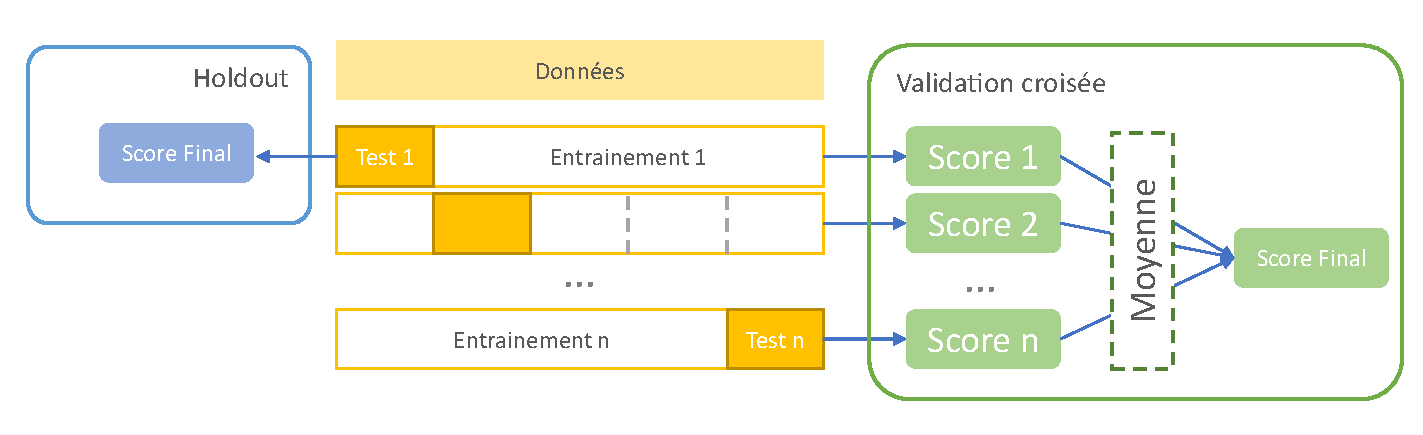
\includegraphics[width=\textwidth]{contents/chapter_3/resources/scheme_holdout_cv.pdf}
    \caption{Schéma des principes des deux approches majeures d'évaluation de modèles. A gauche, la méthode de « holdout » ; A droite, la méthode de validation croisée.}
    \label{fig:scheme_holdout_cv}
\end{figure}

Dans ce travail, nous nous intéressons à la technique de validation croisée ainsi qu'à la valeur moyenne renvoyée par celle-ci. Afin de rendre l'information plus complète, nous calculons également la valeur de l'écart-type à partir des évaluations réalisées sur les divers échantillons, jugée fiable afin de mesurer la stabilité du processus vis-à-vis des données~\cite{Kim2009}. La plupart des travaux ayant recours à la validation croisée emploient une valeur $k$ de 5, jugée suffisante pour l'obtention de valeurs de moyenne et écart-type dans un temps de calcul raisonnable. Néanmoins, il est possible d'amener ce principe à l'extrême en choisissant la plus petite valeur possible pour un lot dédié à l'évaluation soit la taille d'une donnée. Cette valeur $k$ devient égale au nombre de données à traiter, nous basculons alors dans un schéma qualifié de \textit{leave-one-out} ou littéralement "en laisser un de côté".\par

Par ces deux méthodes nous répondons à la problématique de l'évaluation, mais n'apportons pas de solution quant au choix des hyperparamètres. En effet, utiliser un schéma de validation croisée pour régler et évaluer les modèles conduit inévitablement à surestimer les performances du modèle~\cite{Tsamardinos2014}. Ce type de démarche revient à ajuster au mieux une courbe à un nuage de points tout en affirmant que ces mêmes données correspondent à des données inconnues. L'une des solutions à ce problème est l'utilisation d'un double schéma de validation, dont l'un des plus fonctionnels actuellement est celui de la validation croisée imbriquée~\cite{Cawley2010}. Le principe de cette méthode est schématisé sur la \Cref{fig:scheme_hyperparameter_process}, dans laquelle nous retrouvons~:
\begin{itemize}
    \item une boucle \textbf{externe}, permettant d'évaluer un modèle à partir de données de \textbf{test},
    \item une boucle \textbf{interne}, permettant de valider un modèle et ses réglages à partir de données de \textbf{validation}.
\end{itemize}\par
  
\begin{figure}[H]
    \centering
    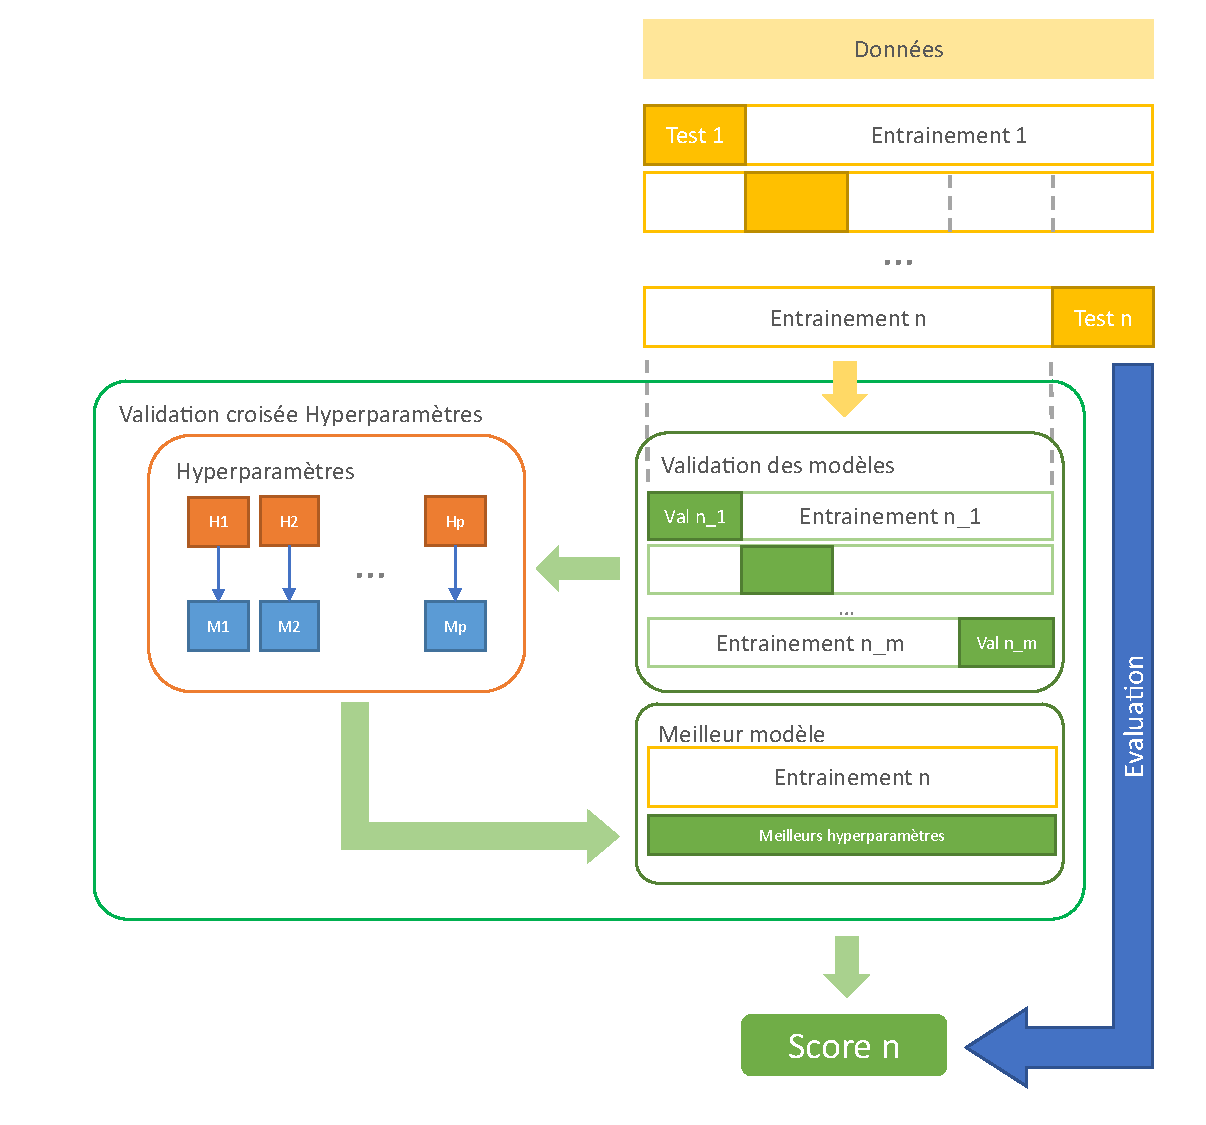
\includegraphics[width=0.9\linewidth]{contents/chapter_3/resources/scheme_hyperparameter_process.pdf}
    \caption{Schéma de la validation croisée imbriquée assurant le choix de la meilleur combinaison d'hyperparamètres et assurant une évaluation robuste des performances du modèle.}
    \label{fig:scheme_hyperparameter_process}
\end{figure}\par

\clearpage

\section{Fusion d’informations}
\label{sec:fusion_information}
Dernier aspect de notre sujet, la fusion d’informations se définit comme l’action de "combiner des informations issues de plusieurs sources afin d’améliorer la prise de décision" ~\cite{Bloch2003}. Cette fusion se retrouve dans de nombreux domaines d'applications dont celui de la santé ou encore de la biométrie, et peut être considérée comme un moyen d'augmenter la fiabilité de systèmes. L'intérêt croissant pour ce domaine correspond, entre autres, à une réponse de l'augmentation et de la diversification du nombre de capteurs présents. L'ouvrage de Bloch~\cite{Bloch2003} justifie la fusion d'informations, par différentes notions auxquelles sont soumises chaque capteur, dont~:
\begin{itemize}
    \item \textbf{l'incertitude}~: c'est à dire son "degré de conformité avec la réalité".
    \item \textbf{l'imprécision}~: définie comme une "mesure du défaut quantitatif de connaissance, sur une mesure".
    \item \textbf{l'incomplétude}~: correspond à "l'absence d'information d'une source sur des aspects du problème".
\end{itemize}\par

Cette fusion est indispensable pour permettre la réalisation de certaines tâches, l'effet de McGurk est un exemple concret de la \textit{complémentarité} de la vision et de l'audition dans le rôle de la perception de la parole, mais également de la difficulté à gérer les \textit{conflits} d'informations sur ces deux sources séparées~\cite{Mcgurk1976}. L'ouvrage de Bloch~\cite{Bloch2003} définit trois termes propres à cette fusion~:
\begin{itemize}
    \item \textbf{le conflit}~: l'une des notions pouvant conduire à une mauvaise interprétation du système lorsque plusieurs informations contradictoires sont reçues.
    \item \textbf{la redondance}~: l'apport multiple d'une même information, pouvant dans l'idéal permettre de réduire les incertitudes et les imprécisions.
    \item \textbf{la complémentarité}~: généralement des sources, liée à un apport de caractéristiques différentes permettant l'accès à une information globale et de lever des ambiguïtés.
\end{itemize}\par

Il est nécessaire également de caractériser le résultat de la fusion d'informations. Il est relativement difficile d'obtenir une vision commune sur les divers niveaux et termes associés. Ainsi, ce travail se réfère à l'une d'entre elles~\cite{Dasarathy1997} proche de notre problématique. Trois niveaux de fusion y sont décris~:
\begin{itemize}
    \item le \textbf{niveau bas}, considéré comme étant la fusion sur les données,
    \item le \textbf{niveau moyen}, considéré comme la fusion des caractéristiques ou données plus abstraites,
    \item le \textbf{niveau haut}, considéré comme la fusion des décisions.
\end{itemize} Niveaux au sein desquels le processus de fusion d'informations peut aboutir à~:
\begin{inlinerate}
    \item une sélection,
    \item une transformation,
    \item une extraction,
    \item ou encore une classification de l'information.
\end{inlinerate} La \Cref{fig:scheme_overview_fusion} propose une schématisation macroscopique de ce concept.\par
 
\begin{figure}[H]
    \centering
    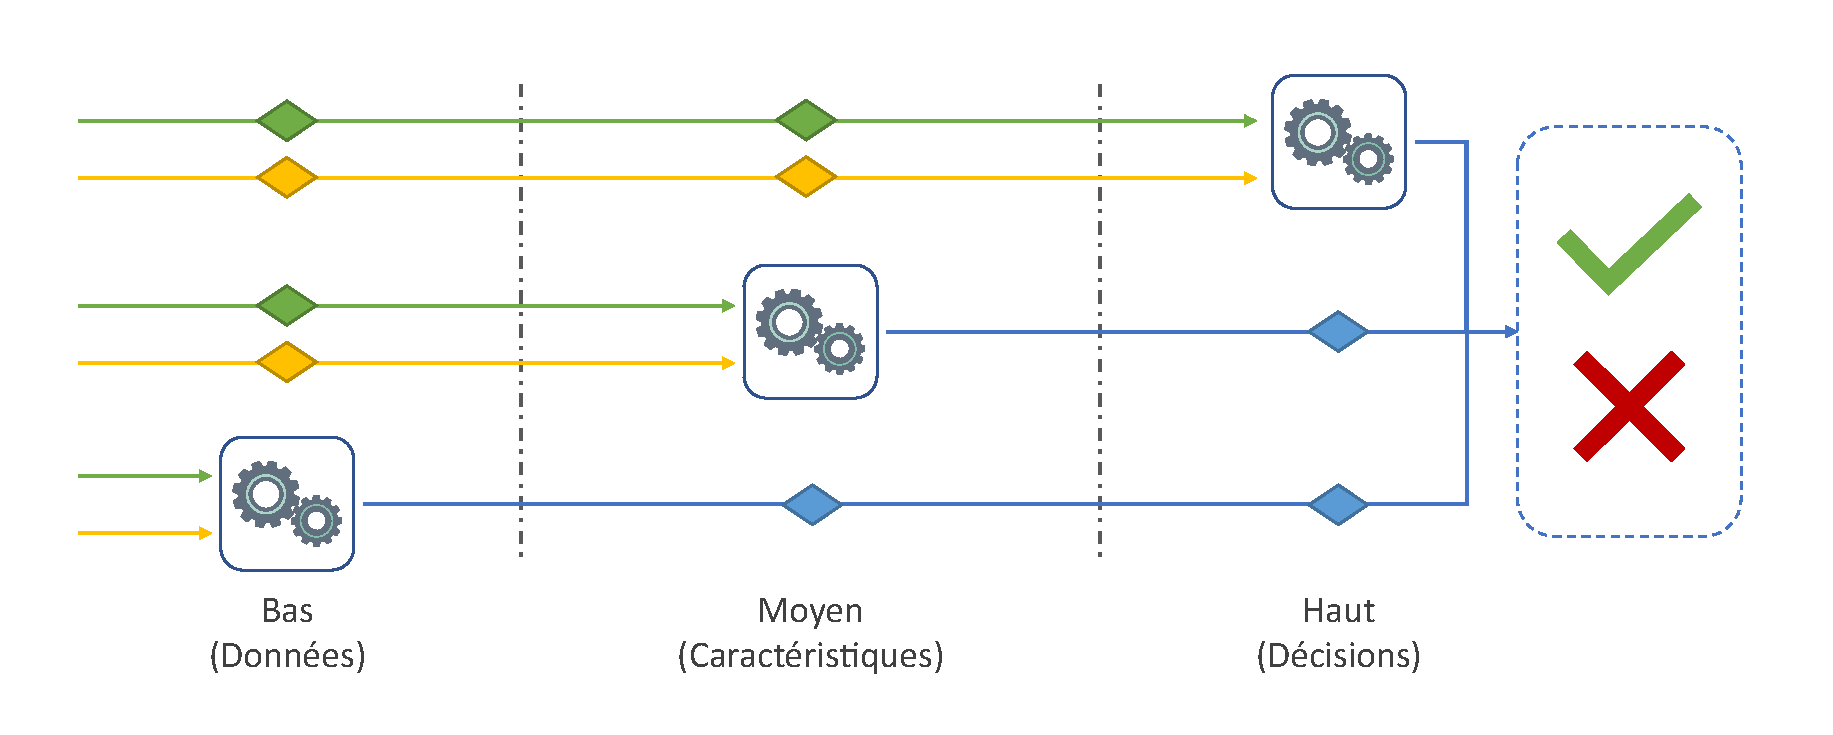
\includegraphics[width=\linewidth]{contents/chapter_3/resources/scheme_overview_fusion.pdf}
    \caption{Schéma des différents niveaux théoriques de fusion sur un schéma multimodal à deux capteurs. Le niveau bas représente le niveau le plus proche des données et des capteurs, le niveau moyen représente le niveau au plus proche de l'extraction de caractéristiques avancées, enfin le niveau haut représente le niveau de prise de décision.}
    \label{fig:scheme_overview_fusion}
\end{figure}\par

La fusion à \textbf{bas niveau} s'exerce au niveau du capteur, quand celui-ci bénéficie de plusieurs relevés d'informations physiques, ou après l'acquisition de données provenant de plusieurs capteurs. Cela va nécessiter une cohérence entre ces modalités~: un référentiel, un repère commun permettant la mise en parallèle de ces dernières. La fusion à ce niveau consiste essentiellement à fournir une cohérence de ces modalités d'information, voire à réduire cette dernière afin de n'obtenir que celle jugée pertinente dans le cadre de son utilisation.\par

La fusion à \textbf{moyen niveau} s'exerce au niveau de caractéristiques, c'est à dire après un premier traitement de chacune des modalités pour n'extraire que les éléments nécessaires à la réalisation du processus. Il s'agit d'une mise en commun des vecteurs d'information dans leur totalité ou réduite nécessitant dans ce second cas une sélection de l'information pertinente.\par

Enfin, la fusion à \textbf{haut niveau} s'exerce après les mécanismes de prise de décision. C'est à dire que les branches correspondant à chaque modalité exercent indépendemment leur prise de décision. Il est donc nécessaire de définir une stratégie permettant de privilégier une décision ou d'extraire une décision à partir de l'information. Deux catégories sont ainsi identifiables~: 
\begin{inlinerate}
    \item la \textbf{sélection dynamique de modèle} de prédiction dans lequel l'objectif est de définir le modèle pertinent,
    \item et la \textbf{fusion de modèles} de prédiction dans lequel le but est d'obtenir une décision globale tenant compte des différentes décisions.
\end{inlinerate}\par

Plus particulièrement, dans le cadre de problématique binaire, la fusion de modèle comporte deux niveaux conceptuels de décision basés sur le type d'information mise à disposition par ces modèles. D'une part, au plus haut niveau~: la fusion appliquée au \textbf{niveau décisionnel}. Seules les décisions issues de chaque modèle sont alors considérées selon diverses stratégies~: le vote à la majorité ou encore la pondération des votes en sont deux représentants. D'autre part, au plus bas niveau~: la fusion appliquée aux scores~\cite{Kittler1998}. Dans le cadre de problématiques à plusieurs classes, nous pouvons évoquer une troisième prise de décision au niveau du rang, c'est à dire en considérant la position de chaque classe prédite issue des divers modèles.\par


% \subsection{Équilibrage de données}
% Nous regroupons au travers de ce terme l’ensemble des problématiques relatives à notre jeu de données et à la représentation de ses classes. Dans le cas de pathologie de la peau, cela peut se caractériser par un jeu de données composé de 100 éléments dont 20\% d’entre elles se réfèrent à des patients atteints de mélanomes et le reste à des patients sains. Nous constatons dans ce cas un déséquilibre entre les classes de ce jeu de données, qu’il nous faudra prendre en compte. Un tel jeu de données peut être qualifié de « non balancés », la répartition de ses classes n’étant pas égale en proportions.
% En effet, certains algorithmes de prédictions peuvent être biaisés, comme par exemple « l’algorithme des plus proches voisins » qui se composera de zones de forte densité privilégiant les données présentes en masse (exemple Figure 37). Un autre biais est également présent lors de l’extraction de métriques pour juger de la pertinence d’un modèle. En effet, dans le cas d’un classifieur qui prédirait constamment « sain », nous obtiendrons un score de 80\% de précision sur notre jeu de données précédent.
  
% \begin{figure}[H]
%     \centering
%     \includegraphics[width=\linewidth]{contents/chapter_3/resources/unbalanced.pdf}
%     \caption{Illustration du problème de données non balancées sur l’algorithme KNN. La densité des données bleu étant supérieure, des prédictions à la frontière de nos deux classes favorisent la classe bleue.}
%     \label{fig:unbalanced}
% \end{figure}

% Plusieurs méthodes existent dans la littérature, pour permettre de rétablir l’équilibre entre les différentes classes. Nous pouvons citer les deux principaux~:
% 	Le sur-échantillonnage, c’est-à-dire que nous gonflons les classes sous représentatives de manière à égaliser la population de la classe majoritaire (en créant de nouveaux éléments artificiels par exemple).
% 	Le sous-échantillonnage, c’est-à-dire que nous réduisons la population de l’ensemble des classes à celle de la classe minoritaire.
 
% \begin{figure}[H]
%     \centering
%     \includegraphics[width=\linewidth]{contents/chapter_3/resources/example_balancement_strategies.pdf}
%     \caption{Représentation de deux principales catégories de stratégie de balancement des données. Le suréchantillonnage tente d’augmenter la taille du jeu de données faible tandis que le sous échantillonnage tend à réduire la classe majoritaire. }
%     \label{fig:example_balancement_strategies}
% \end{figure}
\chapter{État de l'art}
\label{chap:chapter_31}
\chapterintro
Après avoir présenté les trois domaines impliqués dans ce travail, nous allons procéder à la présentation des données qui nous ont servi de base à la réalisation de ces travaux, ainsi que les méthodes cliniques et d'aide au diagnostic de la littérature.\par

Dans un premier temps, nous traiterons de la "matière" utilisée afin de mener cette recherche dans la \Cref{sec:clinical_data}. En effet, l'ensemble de ce travail prend appui sur une base de données mise à disposition initialement pour la réalisation d'une étude clinique menée sur la pertinence de la dermatoscopie et de la \gls{rcm} en milieu clinique~\cite{Cinotti2018}. Nous débuterons par une présentation de l'étude clinique en décrivant les conditions d'inclusions des patients, les dispositifs d'acquisition et le protocole d'évaluation des experts et nous aborderons ces aspects de structuration de la base nécessaire à son utilisation dans le reste de ce document.\par

Dans un second temps et dernier temps, nous procéderons d'une part à un état de l'art clinique des méthodes proposées par la littérature au sein de la \Cref{sec:clinical_methods} et uniquement sur les trois modalités en notre possession, et d'autre part procéderons à un état de l'art similaire consacré cette fois ci aux méthodes d'aide au diagnostic en \Cref{sec:cad_methods} pour les même modalités.\par
\newpage

\section{Données de travail}
\label{sec:clinical_data}
Cette base a reçu une autorisation de la part du comité d'éthique du \gls{chuse} pour son exploitation au sein de l'étude clinique mentionnée précédemment mais également pour ce travail universitaire (numéro du comité d'examen institutionnel 672016/CHUSTE).\par

Cette base de données compile des lésions faciales possédant les critères suivants~:
\begin{itemize}
    \item les images proviennent de patients inclus entre les années 2011 et 2015, dont les données ont exclusivement été acquises au \gls{chuse},
    \item les données sont disponibles pour chaque patient sous 3 formes que sont la photographie clinique, la dermatoscopie et la \gls{rcm} (multimodales),
    \item les lésions considérées dans cette base sont celles dont le diagnostic différentiel, c'est à dire par élimination méthodique des causes (voir
    \Cref{subsec:lentigo}), était fortement controversé et supposé comme étant un \gls{lm} ou \gls{lmm}.
\end{itemize}\par

En terme de composition, la base regroupe 201 patients répartis entre 96 femmes et 105 hommes d'un âge moyen égal à 70 ans compris entre 29 et 97 ans comme présenté sur la \Cref{fig:statistics_age_sex}. Cette base comporte 223 lésions uniques dont le diagnostic que nous utiliserons comme référence provient de l'histologie. Ainsi, nous avons à notre disposition~:
\begin{itemize}
    \item 115 \textbf{lésions malignes}, scindée en 92 \gls{lm} et 23 \gls{lmm},
    \item 108 \textbf{lésions bénignes}, dont 20 \gls{bcc}, 37 \gls{sl}, 23 \gls{sk}, 15 \gls{pak}, 8 nævus, 2 kératoses lichénoïde, 2 cicatrices et 1 maladie de Bowen pigmentée.
\end{itemize}\par

\begin{figure}[H]
    \centering
    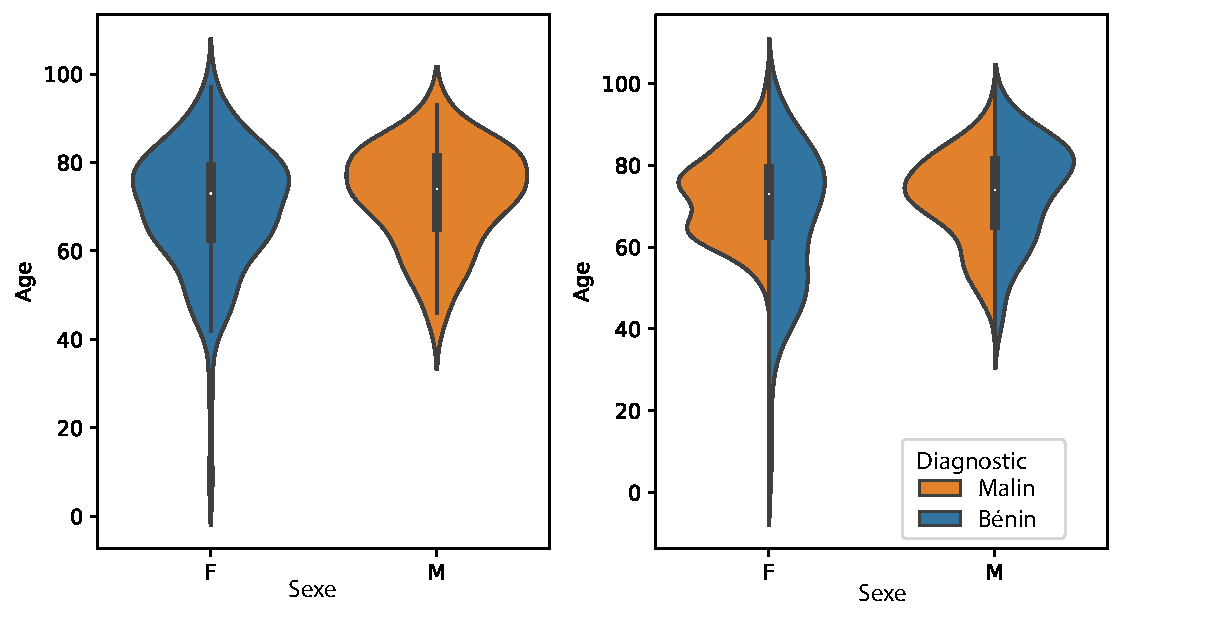
\includegraphics[width=0.8\linewidth]{contents/chapter_3_1/resources/statistics_age_sex.pdf}
    \caption{A gauche, répartition en fonction de l'âge et du sexe. A droite, répartition entre l'âge et le sexe en tenant compte du diagnostic binaire.}
    \label{fig:statistics_age_sex}
\end{figure}\par

Les acquisitions ont été à chaque fois réalisée par l'un des 3 experts investigateurs de l'étude clinique~\cite{Cinotti2018}. Tout cas de collisions de tumeurs au sein d'un même groupe a été exclu de cette étude. En ce qui concerne la modalité de dermatoscopie, les données ont été produites à l'aide d'une caméra PowerShot® G7~\textsuperscript{\ref{footnote:device_powershot}} couplée au dispositif proposé par Fotofinder~\textsuperscript{\ref{footnote:device_fotofinder}}. Pour ce qui est de la modalité de \gls{rcm}, les données proviennent d'un VivaScope 3000®~\textsuperscript{\ref{footnote:device_mavig}}. En revanche, aucune information liée à l'acquisition des données de photographie clinique n'a été mentionnée.\par

L'intérêt de ces trois modalités est grand dans le contexte de la dermatologie puisqu'elles représentent le processus "classique" de prise en charge clinique, de la modalité la moins onéreuse avec la \textbf{photographie clinique} mais également la moins précise, à des modalités plus onéreuses, également plus riche en information, avec la \textbf{\gls{rcm}}. Ainsi, chaque modalité permet au praticien de réduire la zone d'incertitude chez un patient souffrant d'une pathologie de la peau.

\addtocounter{footnote}{1}
\footnotetext[\thefootnote]{Source~: Canon Powershot®, Canon, Tokyo, Japon. \label{footnote:device_powershot}}
\addtocounter{footnote}{1}
\footnotetext[\thefootnote]{Source~: FotoFinder Systems GmbH, Bad Birnbach, Allemagne. \label{footnote:device_fotofinder}}
\addtocounter{footnote}{1}
\footnotetext[\thefootnote]{Source~: Distribué en Europe par MAVIG GmbH, Munich, Allemagne. \label{footnote:device_mavig}}

Afin d'évaluer les performances de praticiens face à ces lésions, les investigateurs ont eu recours à 21 dermatologues détenant une expertise des modalités d'imagerie non-invasives. Ces experts sont répartis de manière homogène selon leurs compétences respectives pour chacun des dispositifs. Ainsi, le panel d'évaluation se décompose de la façon suivante~: 
\begin{inlinerate}
    \item 6 experts sont soumis à l'ensemble des modalités,
    \item 15 experts sont soumis à l'évaluation de la photographie clinique et de la dermatoscopie (dont 9 uniquement dédiés a ces deux modalités),
    \item et 12 sont soumis à la \gls{rcm} (dont 6 uniquement dédiés à la \gls{rcm})~\cite{Cinotti2018}.
\end{inlinerate}
La répartition de ces experts est résumée en \Cref{fig:experts_evaluation}.\par

\begin{figure}[H]
    \centering
    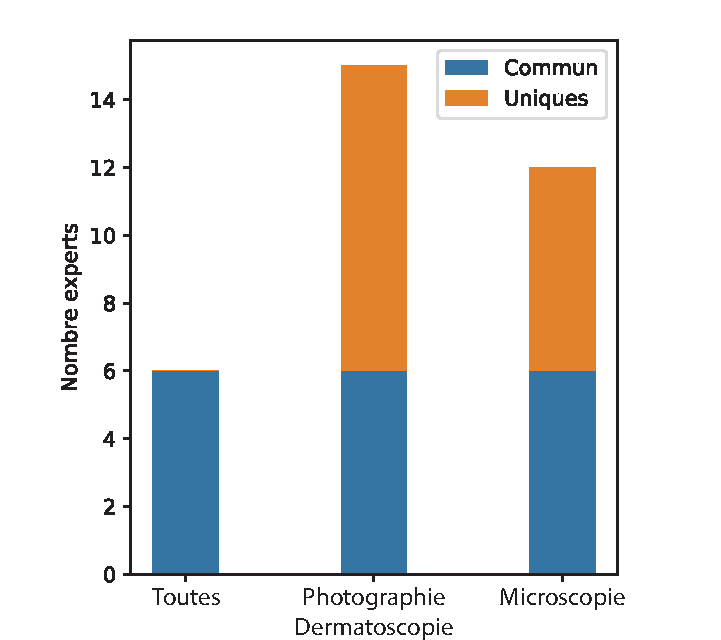
\includegraphics[width=0.6\linewidth]{contents/chapter_3_1/resources/experts_evaluation.pdf}
    \caption{Répartition du panel de 21 dermatologues sur l'évaluation des diverses modalités~\cite{Cinotti2018}.}
    \label{fig:experts_evaluation}
\end{figure}\par

Ces experts ont évalué la gravité pour chaque cas clinique présenté selon les termes bénin et malin. Afin d'éviter un biais de la part des experts qui ont réalisé l'évaluation sur les 3 modalités, ceux-ci ont été sollicités sur trois journées différentes~: 
\begin{inlinerate}
    \item une première journée d'évaluation ne comprenant que les images de photographie clinique et de dermatoscopie,
    \item une seconde journée d'évaluation ne comprenant que les images de \gls{rcm},
    \item et une dernière journée d'évaluation sur l'ensemble de la base d'images.
\end{inlinerate}
Par ailleurs, les cas cliniques ont été présentés dans un ordre différent entre chaque journée d'évaluation afin d'éviter des biais liés à l'activité précédente des experts.\par

La base d'images utilisée pour cette évaluation nous été remise, et ses données sensibles ont été anonymisée afin de ne pas pouvoir ré-identifier les patients. La structure de cette base peut être appréhendée sur la \Cref{fig:db_structure} - Gauche, et se compose~:
\begin{itemize}
    \item d'un \textbf{tableau de lésions}, sous forme de fichier \gls{csv} et contenant~:
    \begin{itemize}
        \item \textbf{en colonne}, les diverses informations relatives au patient, soit \textit{l'âge, le sexe, la zone, son diagnostic binaire issu de l'histologie (malin ou bénin) et diagnostic précis},
        \item \textbf{en ligne}, les divers enregistrements liés à chaque lésion respectant les champs précisé en colonne.
    \end{itemize}
    \item d'un \textbf{répertoire d'images} comprenant les divers cas clinique recensés dans l'étude sous divers formats image.
\end{itemize}\par

Afin d'exploiter au mieux cette base, quelques modifications ont été apportées. D'une part, la diversité des formats images est un frein quant à la gestion de ces données et nous avons opté pour un format matriciel sans perte de type bitmap. D'autre part, la structure de la base dans l'état ne permettait pas l'utilisation d'annotations au niveau des images ou supplémentaires à d'autres niveaux. Afin de rendre plus dynamique cette partie, nous avons opté pour une structure reprenant le tableau des lésions initial, lié à des répertoires associés à chaque lésion. Ce procédé est ainsi répété de manière récursive, chaque dossier de lésion se compose lui même de tableaux d'annotations propre au type d'annotations stockées. Par ailleurs, certains apports d'informations ont été réalisés pour permettre un bon déroulement de la suite de notre travail, tel que l'appartenance à un patient afin de ne pas proposer des données d'un même patient lors de l'entraînement et du test. La \Cref{fig:db_structure} - Droite synthétise la structure de cette base après modification.\par

\begin{figure}[H]
\centering
    \begin{subfigure}{.45\textwidth}
      \centering
      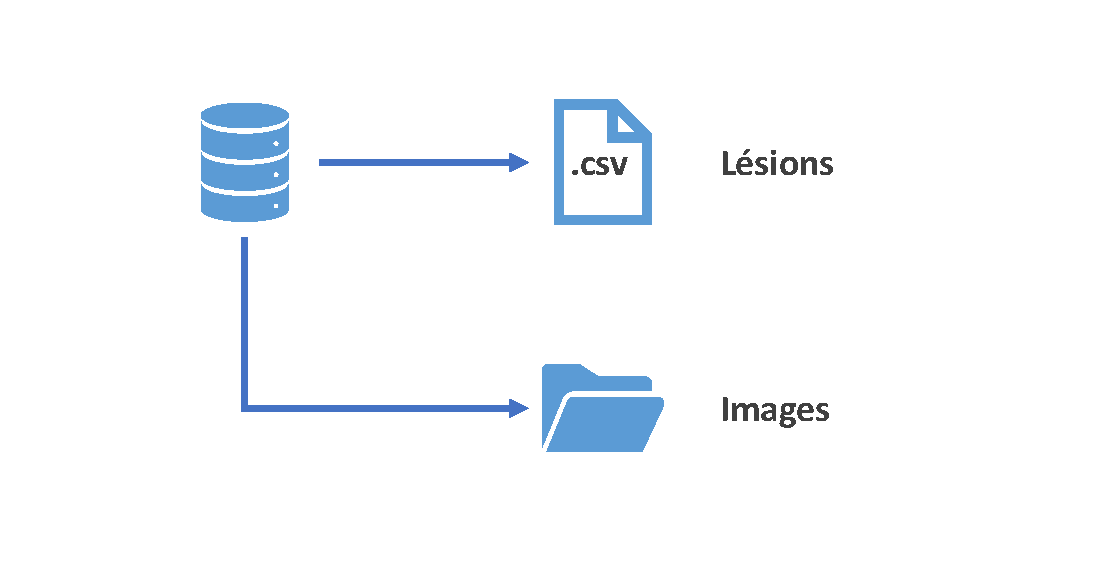
\includegraphics[width=\linewidth]{contents/chapter_3_1/resources/scheme_dbstructure_old.pdf}
    \end{subfigure}
    \begin{subfigure}{.45\textwidth}
      \centering
      \includegraphics[width=\linewidth]{contents/chapter_3_1/resources/scheme_dbstructure_new.pdf}
    \end{subfigure}
    \caption{Schéma de l'organisation de la base de ressources employée. A gauche, la base initiale et à droite, la base restructurée afin de supporter de nouvelles annotations.}
    \label{fig:db_structure}
\end{figure}\par

\section{Méthodes clinique}
\label{sec:clinical_methods}
Pour permettre l'identification de pathologie en dermatologie plus routinière, la mise en avant de critères de diagnostic est une démarche clé permettant de rendre cette tâche plus efficace. Cette mise en avant de critères à été débutée au milieu des années 1980, sous la forme:
\begin{itemize}
    \item d'\textbf{acronyme}: l'idée est de proposer une méthode de diagnostic facile à mémoriser. Le travail de Friedman est un exemple, bien que révisé, le critère ABCD(E) est encore utilisé et applicable par de nombreuses personnes expertes ou non~\cite{Friedman1985}.
    \item de \textbf{liste}: de critères positifs et négatifs, correspondant à des caractéristiques rédhibitoires ou non, et amenant à un score final. Ce score variera selon la pathologie considérée et permettra d'en déduire une décision à prendre. L'un des exemple dans le cadre de lésions pigmentées est celui de MacKie en 1986~\cite{mackie1986}. Ces critères ont été révisés et se destinent néanmoins à un public expert. 
\end{itemize}\par

Ces démarches "algorithmiques" de diagnostic, ainsi nommées, se sont progressivement étendues à d'autre pathologies et dispositifs d'analyse médicaux. Ils permettent de se référer à des critères essentiels en cas de doute. Le \gls{rcm} n'est pas exempt de ces démarches simplifiées, notamment pour le diagnostic du \gls{lm} avec les travaux de Pellacani et Guitera~\cite{Pellacani2007, Guitera2010}. Ces deux travaux proposent sous forme de table de critères ceux jugés positifs et négatifs, dont la \Cref{tab:rcm_algorithm_lentigo} donne un aperçu de la production de ces articles. Leur étude comptabilise 81 cas de \gls{lm} et 203 lésions bénignes, sur lesquels un seuil de score de 2 a été jugé comme pertinent au regard de l'étude statistique menée. Celui-ci a permis de détecter avec 85\% de sensibilité et 76\% de spécificité les \gls{lm}.\par

\begin{table}[H]
\centering
    \begin{tabular}{ll}
        \toprule
        Type de caractéristiques                        & Caractéristiques                                              \\\hline
        \multirow{2}{*}{Positives Majeures (+2 points)} & Papilles à contour faiblement définis                         \\\cline{2-2}
                                                        & Cellules pagétoides rondes >\SI{20}{\micro\metre}             \\\hline
        \multirow{3}{*}{Positives Mineures (+1 points)} & Présence de cellules atypiques dans la \gls{dej}              \\\cline{2-2}
                                                        & Combinaison de follicule / cellules atypique / pagétoide      \\\cline{2-2}
                                                        & Présence de cellules nucléée au sein de papilles              \\\hline
        Négatives Mineures (-1 points)                  & Motif en alvéoles larges                                      \\
        \bottomrule
    \end{tabular}
\caption{Caractéristiques observables par \gls{rcm} jugées pertinentes pour la détection du \gls{lm}~\cite{Guitera2010}.}
\label{tab:rcm_algorithm_lentigo}
\end{table}\par
 
Ainsi, une caractéristique a été déterminée comme pertinente par leurs auteurs~\cite{Pellacani2007, Guitera2010} lorsque celle-ci s'exprimait de manière plus significative dans l'un des deux groupes pathologiques (\gls{lm} ou bénin). L'un de ces travaux~\cite{Guitera2010} procède à une analyse de ces caractéristiques par profondeur croissante de la peau, dont nous listons quelques uns des éléments majeurs~:
\begin{itemize}
    \item au niveau de \textbf{l'épiderme}, les auteurs ont constaté que les pathologies de \gls{lm} comportent un désordre des cellules de l'épiderme (56\% des lésions \gls{lm} contre 18\% des lésions bénignes). Également, une infiltration pagétoïde a été reportée dans la plupart des cas de \gls{lm} (75\% des lésions \gls{lm} contre 28\% des lésions bénignes). En opposition, un épiderme homogène, caractérisé par des motifs en nids d'abeille, ont été constatés dans 92\% des cas bénins. Ces éléments peuvent être observées sur la \Cref{fig:example_rcm_pattern_1}.
    \item au niveau de la \textbf{\gls{dej}}, les auteurs ont constaté que les papilles non démarquées étaient observées dans la majorité des \gls{lm} (68\% \gls{lm} and in 17\% des cas bénins). Ces éléments peuvent être observées sur la  \Cref{fig:example_rcm_pattern_2}.
    \item au niveau du \textbf{derme}, 15\% des cas de \gls{lm} présentent des cellules nuclées large contre 2\% des lésions bénignes. Ces élements peuvent être observées sur la \Cref{fig:example_rcm_pattern_3}.
\end{itemize}\par

\begin{figure}[H]
    \begin{center}
        \includegraphics[width=0.9\linewidth]{contents/chapter_3_1/resources/example_rcm_pattern_1.pdf}
        \caption{Cas de données cliniques \gls{rcm} en provenance de l'épiderme par Guitera~\cite{Guitera2010}. En a) et b), exemples de motifs en large nids d'abeille (\textit{broadened honeycomb pattern}), respectivement d'un kératose séborrhéique et de peau normale ; en c), exemples de motifs de pavés atypiques (\textit{atypical cobblestone pattern}) issus d'un \gls{lm} ; en d), exemples de \textit{large pagetoid} cellules propre au \gls{lmm}. Repère~: barre = \SI{50}{\micro\metre}.}
        \label{fig:example_rcm_pattern_1}
    \end{center} 
\end{figure}\par

\begin{figure}[H]
    \begin{center}
        \includegraphics[width=0.7\linewidth]{contents/chapter_3_1/resources/example_rcm_pattern_2.pdf}
        \caption{Cas de données cliniques \gls{rcm} par Guitera~\cite{Guitera2010}. En a) et au niveau de la flèche, exemple de papille à frontière non marqué (\textit{Nonedge papillae}) et de cellules atypique d'un \gls{lm} acquise à la jonction \gls{dej} ; En b), exemple de papilles à frontières marquées (\textit{Edge papillae}) d'une pathologie bénigne. En c), exemple de cellules atypiques au niveau de la \gls{dej} typique de \gls{lm} ; En d), exemple de halo noir autour de cellules atypiques de l'épiderme issue d'un \gls{lm}. Repère~: barre = \SI{50}{\micro\metre}.}
        \label{fig:example_rcm_pattern_2}
    \end{center} 
\end{figure}\par

\begin{figure}[H]
    \begin{center}
        \includegraphics[width=0.8 \linewidth]{contents/chapter_3_1/resources/example_rcm_pattern_3.pdf}
        \caption{Cas de données cliniques \gls{rcm} par Guitera~\cite{Guitera2010}. En a), exemple de cellules atypiques à proximité d'un follicule pileux au sein de la \gls{dej} sur un \gls{lm} ; En b), exemple de cellules nucléé du derme d'un \gls{lm}. Repère~: barre = \SI{50}{\micro\metre}.}
        \label{fig:example_rcm_pattern_3}
    \end{center} 
\end{figure}\par

Dans l'étude menée par Cinotti et al.~\cite{Cinotti2018}, les auteurs investigateurs ont demandé d'évaluer certaines caractéristiques récurrentes de la littérature, parmi lesquelles~:
\begin{itemize}
    \item la présence de grandes cellules pagétoïdes arrondies, présentes dans 37\% des \gls{lm} et seulement 5\% des pathologies bénignes,
    \item la présence de grandes cellules dendritiques dans l'épiderme, présentes dans 81\% des \gls{lm} contre 13\% des pathologies bénignes,
    \item la localisation au niveau des follicules pileux des cellules atypiques, dans 62\% des \gls{lm} et seulement 7\% des pathologies bénignes.
\end{itemize}\par

\section{Démarches d'aide au diagnostic}
\label{sec:cad_methods}

\cite{Wiltgen2008}
\cite{Halimi2017a}





% Part 2
\part{Analyse de la microscopie confocale par réflectance}
\label{part:microscopy}
\renewcommand{\thechapter}{\roman{chapter}}
\setcounter{chapter}{2}
\setcounter{figure}{0}

\unchapter{Préambule microscopie confocale par réflectance}
\label{chap:preamble_microscopy}
La précédente partie de ce travail consacrée au contexte, permet une mise en situation des connaissances mobilisées et une présentation des recherches liées à celui-ci. Au sein de cette seconde partie est élaborée une méthodologie destinée à la modalité \acrlong{mcr}. Cette recherche est motivée par diverses raisons. En premier lieu, il s'agit de l'une des modalités les plus précises à disposition du spécialiste en condition clinique. Cette modalité représente une référence en matière de qualité de diagnostic à réaliser. En second lieu, cette recherche est motivée par le nombre restreint de travaux menés sur le diagnostic de lésion de la peau appliqué à la modalité de \gls{mcr} et assisté par ordinateur. En effet, cette modalité représente un verrou scientifique qu'il est nécessaire de lever pour accomplir le schéma de diagnostic multimodal. Ce préambule a pour objectif de présenter d'une part les données de travail exclusives à la modalité de \gls{mcr} introduites lors du \Cref{chap:chapter_4}, et d'autre part de présenter les résultats des experts qui constituent la finalité des méthodes d'aide au diagnostic de cette partie.\par

Ainsi dans cette partie, seules les données \gls{mcr} des 224 lésions mises à disposition sont considérées \textbf{pour l'évaluation} des méthodes et sont exclues les images de photographie clinique et de dermatoscopie. Pour rappel, ces données correspondent à des lésions pouvant porter à confusion lors du diagnostic de \gls{lm} et de \gls{lmm} par le spécialiste. En addition à ces données, 28 patients bénins non présents dans la base d'images initiale sont utilisés afin d'augmenter le nombre d'images annotées comme bénignes \textbf{pour l'entraînement} des méthodes développées.\par

Chaque lésion contient des images \gls{mcr} jugées pertinentes par deux des trois médecins investigateurs dont l'acquisition des images provient de la \gls{jde}. En effet, ces deux pathologies sont observables à ce niveau de profondeur~:
\begin{itemize}
    \item les \textbf{pathologies de \gls{lm}} résultent d'une prolifération de cellules au niveau de la lame basale (extrémité supérieure de la \gls{jde}),
    \item les \textbf{pathologies de \gls{lmm}} résultent de l'intrusion de la mélanine se propageant le long des follicules pileux (extrémité supérieure et intérieur de la \gls{jde}).
\end{itemize} Ces images dont l'acquisition est réalisée au niveau de la \gls{jde} sont donc ainsi parfaitement adaptées à la caractérisation de ce phénomène par les médecins.\par

Du point de vue des caractéristiques, ces images arborent une taille constante de \SI{1000}{\px} $\times$ \SI{1000}{\px} pour une section mesurée de \SI{920}{\micro\metre} $\times$ \SI{920}{\micro\metre} et une résolution en profondeur comprise entre \SI{3}{\micro\metre} et \SI{5}{\micro\metre}. Ces données fournissent ainsi une résolution de \SI{1}{\micro\metre}. Les informations d'acquisition (profondeur, longueur d'onde, \ldots) contenues dans les images ne pourront être utilisées car non exploitables (procédure de calibration non réalisée, informations manquantes, \ldots).\par
\clearpage

À partir de ces données, l'analyse menée par les 12 experts en \gls{mcr} de l'étude~\cite{Cinotti2018} permet d'obtenir une valeur moyenne de sensibilité de 0,84 $\pm$ 0,05 et une valeur moyenne de spécificité de 0,75 $\pm$ 0,06 sur l'évaluation des pathologies malignes toutes confondues. Sur l'évaluation des données de \gls{lm} et \gls{lmm}, ces scores deviennent plus homogènes avec une valeur moyenne de sensibilité de 0,80 $\pm$ 0,07 et une valeur moyenne de spécificité de 0,81 $\pm$ 0,05. Les courbes \gls{roc} associées à ces performances sont représentées sur la \Cref{fig:results_roc_rcm_experts}.\par

\begin{figure}[H]
    \begin{center}
        \includegraphics[width=0.95\linewidth]{contents/ii_preamble_microscopy/resources/results_roc_rcm_experts.pdf}
        \caption{Courbes \gls{roc} issues de l'évaluation des données \gls{mcr} par les 12 experts~\cite{Cinotti2018}. À gauche, le résultat de l'analyse des experts, mené sur la détection d'éléments malins~;~À droite, le résultat de l'analyse des experts, mené sur la détection de \gls{lm} et \gls{lmm}.}
        \label{fig:results_roc_rcm_experts}
    \end{center} 
\end{figure}\par

L'objectif visé par cette partie est d'égaler ces scores à l'aide de méthodes de diagnostic sur base d'images issues de la \gls{mcr}. À ce titre, les méta-données extraites des informations patient (telles que l'âge, le sexe ou encore l'emplacement de la lésion) ne sont pas exploitées, bien que l'âge ait été mis à disposition des experts en \gls{mcr} durant leur évaluation. Ce choix est justifié car contrairement aux connaissances des experts, ces méta-données ne sont pas représentatives de la population réelle et peuvent induire des biais de corrélations sur des données extérieures à la base employée. Ainsi, les évaluations des méthodes ne portent que sur \textbf{l'aspect de vision} de ces données \gls{mcr}.\par

Ainsi, diverses ressources d'intelligence artificielle évoquées lors du \Cref{chap:chapter_3} sont mobilisées lors de ce travail. Des apports ont été réalisés pour permettre le déroulement des expériences présentées lors des chapitres suivants. En effet, la base d'images actuelle ne possède que des annotations au niveau des patients, ce qui limite fortement l'étendue des travaux essentiellement basés sur des méthodes d'apprentissage supervisé. À l'aide d'un outil graphique réalisé pour cette étude (\Cref{fig:example_gui_annotation}) et grâce au travail de l'un des dermatologues investigateurs, divers niveaux d'annotations supplémentaires sont obtenus, dont~:
\begin{itemize}
    \item des annotations au \textbf{niveau des images} correspondant au plus petit niveau issu des données originelles,
    \item des annotations au \textbf{niveau de sous-parties d'images} également appelés \textit{patchs} correspondant à l'extraction d'un nouveau niveau de données à partir des images.
\end{itemize}\par
\clearpage

\begin{figure}[H]
\centering
    \begin{subfigure}{.45\textwidth}
      \centering
      \includegraphics[width=\linewidth]{contents/ii_preamble_microscopy/resources/example_gui_annotation_1.png}
    \end{subfigure}
    \begin{subfigure}{.45\textwidth}
      \centering
      \includegraphics[width=\linewidth]{contents/ii_preamble_microscopy/resources/example_gui_annotation_2.png}
    \end{subfigure}
    \caption{Interface logicielle mise à disposition du spécialiste, afin de procéder aux annotations au niveau des images et des sous-images. À gauche, l'onglet permettant l'annotation au niveau des images~;~À droite, l'onglet permettant la création et l'annotation de sous-images.}
    \label{fig:example_gui_annotation}
\end{figure}

Les annotations au niveau des lésions bien que initialement sur deux classes, donnent naturellement lieu au niveau des images à des annotations sur \textbf{trois classes}. Ces annotations, dont des exemples sont visibles sur la \Cref{fig:example_rcm_data}, sont les suivantes~:
\begin{itemize}
    \item Un premier type d'annotation du nom de \textit{malin} a été apposé \textit{sur des images} contenant \textbf{au moins} du tissu de type malin et \textit{sur des sous-images} contenant essentiellement celui-ci.
    \item Un second type d'annotation du nom de \textit{bénin} a été apposé \textit{sur des images} ne contenant \textbf{aucun} tissus malin mais \textbf{au moins} du tissu bénin et \textit{sur des sous-images} composées de celui-ci.
    \item  Enfin, un troisième type d'annotation du nom \textit{sain} a été renseigné \textit{sur des images} ne contenant \textbf{aucun} des deux types de tissus précédents et \textit{sur des sous-images} composées de tissus sains. 
\end{itemize}\par

La répartition complète de cette base annotée est disponible sur la \Cref{fig:scheme_rcm_statistics} dans laquelle peut être visualisée la composition des annotations de la base d'images au niveau des \textbf{lésions}, des \textbf{images} et des \textbf{sous-images}. D'une part, est visible la répartition des données de \textit{la base de référence} ou \textit{base initiale}~\cite{Cinotti2018} de laquelle est issue \textbf{l'évaluation des experts} mais également servant à \textbf{l'entraînement et l'évaluation des méthodes} qui suivent. D'autre part, est visible la répartition des \textit{données additionnelles} qui servent à \textbf{corriger le non-balancement lors de la phase d'entraînement}.\par

\begin{figure}[H]
    \begin{center}
        \includegraphics[width=0.9\linewidth]{contents/ii_preamble_microscopy/resources/example_rcm_data.pdf}
        \caption{Exemple de tissus et annotations, considérés respectivement de gauche à droite comme \textit{sain}, \textit{bénin} et \textit{malin} par le spécialiste.}
        \label{fig:example_rcm_data}
    \end{center} 
\end{figure}\par

\begin{figure}[H]
    \begin{center}
        \includegraphics[width=0.8\linewidth]{contents/ii_preamble_microscopy/resources/scheme_rcm_statistics.pdf}
        \caption{Répartition des annotations réalisées par l'expert sur lésions, les images et sous-images. En bleu foncé, la base initiale de Cinotti~\cite{Cinotti2018}~;~En bleu clair, les données additionnelles.}
        \label{fig:scheme_rcm_statistics}
    \end{center} 
\end{figure}\par

Afin de répondre à ce besoin de diagnostic au niveau des lésions acquises par \gls{mcr}, cette partie dédiée à cette modalité dans laquelle est développée une méthodologie ascendante se compose de trois chapitres~:
\begin{itemize}
    \item dans un premier temps, le \Cref{chap:chapter_5} aborde la \textbf{prise de décision au niveau de l'image} par des schémas simples permettant une prise de décision sur les images \gls{mcr},
    \item dans un second temps, le \Cref{chap:chapter_6} propose des méthodes destinées à \textbf{améliorer ce diagnostic image} par la mise en oeuvre de schémas avancés permettant à nouveau la prise de décision sur les images \gls{mcr},
    \item enfin, le \Cref{chap:chapter_7} se focalise sur une \textbf{prise de diagnostic au niveau du patient} par la présentation de processus décisionnel au niveau lésionnel.
\end{itemize}\par
\newpage
\renewcommand{\thechapter}{\arabic{chapter}}
\setcounter{chapter}{4}

\chapter{Diagnostic de l'image}
\label{chap:chapter_4}
\chapterintro
Comme évoqué durant le préambule, cette partie s'intéresse au premier niveau de diagnostic de notre processus global sur la modalité \gls{rcm}. Nous traiterons en d'autres termes, de la classification des images de cette modalité. Nous nous intéresserons à leur séparation selon trois annotations : saine, bénigne ou maligne, mais également reviendrons à des considérations d'ordre médical de détection de malignité de ces images.\par

Ainsi, ce chapitre séparera plusieurs aspects dont dans un premier temps l'extraction de caractéristiques pertinentes par des méthodes manuelles mais également auto déterminée à l'aide de réseaux profond pré-entraînés, et dans un second temps la mise en œuvre de méthodes de classification éprouvées. Afin de rendre plus riche cette partie et de compléter nos conclusions, nous nous intéresserons également à l'influence de divers paramètres liés à la normalisation des caractéristiques, à la réduction de l'information dans le contexte de méthodes à fort nombre de dimensions, et à l'influence des données sur les résultats de classification.\par	
\newpage

%%%%%%%%%%%%%%%%%%%%%%%%%%%%%%%%%% 
%%%%%%%%%%%%%%%%% METHODOLOGIE
\section{Méthodologie}
La classification de la peau par méthode d'apprentissage est un problème très largement développé dans la littérature, notamment pour le mélanome. Néanmoins, dans le cadre plus particulier de la détection des \gls{lm} et \gls{lmm} sur base d'images \gls{rcm}, cette problématique n'a été abordé que par quelques articles~\cite{Halimi2017a, Halimi2017b, Wiltgen2008, Koller2011}. Nous nous intéresserons à la détection de cette pathologie au sein de la base d'image mise à disposition, et nous étudierons cette problématique selon divers angles d'approche : 
\begin{inlinerate}
    \item d'une part la séparation des tissus malins, bénins et sains sous forme de problématique à 3 classes,
    \item et d'autre part, nous focaliserons sur la séparation entre les tissus malin et le reste des tissus sous forme de problématique binaire.
\end{inlinerate}\par

Afin de traiter ces problématiques, nous aborderons ces cas à l'aide de méthodes d'apprentissage supervisées, que nous déroulerons lors de ces prochains paragraphes. En effet, ces approches sont largement explorées dans des thématiques variées du domaine de l'images médicale et également démontrées comme fonctionnelles~\cite{Litjens2017,Pathan2018}. Nous aborderons les prochains éléments selon un processus de classification classique, dans lequel nous adapterons certains des traitements en conséquence de notre problématique. Une vision macroscopique est présenté sur le schéma de la \Cref{fig:scheme_macro_image_classification}.\par

Le pré-traitement des images n'est pas considéré dans ce travail, car jugé peu utile sur des images \gls{rcm} et assez peu traité dans la littérature. Nous suivrons ce processus selon trois étapes majeures :
\begin{inlinerate}
    \item l'extraction de caractéristiques,
    \item le pré-traitement avant classification,
    \item et les méthodes de classification.
\end{inlinerate}
Ainsi, nous consacrerons une sous-section pour chacun de ces points lors des prochaines sous-parties. Puis, nous présenterons la méthodologie propre au déroulement de ces expériences et critères d'évaluation, avant de procéder à l'analyse des résultats.\par

\begin{figure}[H]
\centering
    \includegraphics[width=\linewidth]{contents/chapter_4/resources/scheme_macro_image_classification.pdf}
    \caption{Représentation macroscopique du processus de diagnostic image suivi dans le cadre de l'apprentissage automatique. Nous arborerons une démarche la plus compréhensive, à 3 classes - a), mais également binaire par une emphase sur les images malignes - b).}
    \label{fig:scheme_macro_image_classification}
\end{figure}\par

\newpage

%%%%%%%%%%%%%%%%%%%%%%%%%%%%%%%%%% 
%%%%%%%%%%%%%%%%% FEATURES
\section{Extraction de caractéristiques}
\label{chap:feature_extraction}
L'étape d'extraction de caractéristiques consiste en l'obtention de valeurs dérivées à partir des données brutes, dans le but de quantifier un phénomène, jugées pertinents pour la suite du traitement (généralement de la classification). Les éléments présentés en préambule visent à montrer l'importance des motifs de tissus, dont l'apparence varie selon :
\begin{itemize}
    \item \textbf{la profondeur de l'acquisition} du tissus considéré, ainsi l'épiderme, \gls{dej} et le derme sont très différents du point de vue des tissus qui les constituent,
    \item \textbf{la pathologie à identifier}, les différentes lésions en notre possession sont assez différentes selon leur état bénin ou malin.
\end{itemize}
Les nombreux échanges menés auprès des dermatologues de notre étude clinique de référence ont également abouti à vérifier l'importance des aspects de textures au sein de leur processus cognitifs de décision vis-à-vis des pathologies de \gls{lm} et \gls{lmm}.\par

Nous traiterons des techniques d'extraction de caractéristiques appliquées à nos images \gls{rcm}, que nous aborderons selon deux axes :
\begin{inlinerate}
    \item d'une part les techniques d'extraction de caractéristiques manuelles ou déterminées par un humain respectivement séparées en caractéristiques \textit{spatiales} et \textit{fréquentielles},
    \item d'autre part les techniques d'extraction de caractéristiques non manuelles.
\end{inlinerate} 
L'appellation "manuelle" s'est ainsi imposé suite à l'apparition de réseaux de convolution profonds, afin de distinguer ces deux types d'approches~\cite{Nanni2017}.\par

\subsection{Extraction de caractéristiques manuelle spatiales}
L'extraction sur base d'information du domaine spatial est un champ de travail assez développé présentant comme avantage d'être intuitif mais pouvant être affecté par le bruit et autres phénomènes de dégradation de l'information. Ces opérations spatiales peuvent être décrites à deux niveaux d'interprétation, d'une part celui des valeurs brutes dont les descripteurs de premier ordre font partie mais ne fournisse aucune valeur de cohérence spatiale et, d'autre part celui par transformation de l'information initiale dont les descripteurs de second ordre ou plus font partie. Ces dernières méthodes prennent en compte la relation d'une valeur locale à celle de son voisinage~\cite{Kamila2015}.\par

Les descripteurs de premier ordre s'appliquent ainsi aux valeurs d'intensité ou à la distribution de celle-ci, sans traitement préalable. La \Cref{tab:first_order_descriptors} recense la plupart de ces caractéristiques issues de la distribution des valeurs brutes. Néanmoins, ces mesures tendent à ressortir des phénomènes globaux de l'image, mais ne suffisent pas à elles seules à analyser des motifs présent~\cite{Tomita1990, Srinivasan2008, Uyun2013, NyeinNyeinHlaing2015}. Ces mesures ont notamment été utilisées comme un complément de classification~\cite{Wiltgen2008}.\par

\begin{table}[H]
    \centering
    \begin{tabular}{ll}
        \toprule
        \textbf{Mesure}             & \textbf{Expression mathématique}                                                  \\ \hline
        Moyenne                     & $\overline{x} = \frac{1}{n}\sum_{i=1}^n x_i$                                      \\   
        Variance                    & $v = \frac{1}{n}\sum_{i=1}^n \left(x_i - \overline{x}\right)^2$                   \\ 
        Entropie                    & $e = -\sum_{i=1}^n {\mathrm{P}(x_i) \log_b \mathrm{P}(x_i)}$                      \\
        Kurtosis                    & $k=\frac{r \sum_{i=1}^{n}\left(x_{i}-\bar{x}\right)^{4}}{\left(\sum_{i=1}^{n}\left(x_{i}-\bar{x}\right)^{2}\right)^{2}}-3$\\
        Asymétrie                   & $a = \mathbb{E} \left[ \left( \frac{X - \mu}{\sigma} \right)^3 \right]$           \\  
        \bottomrule
    \end{tabular}
    \caption{Liste de différentes mesures obtenues à partir du premier ordre.}
    \label{tab:first_order_descriptors}
\end{table}\par

Les descripteurs de second ordre, ou plus, utilisent l'information locale et en déduisent une relation à leur voisinage par l'utilisation d'une transformation intermédiaire. Parmi ces transformations, les plus courantes d'entre elles sont : 
\begin{inlinerate}
    \item \gls{glcm},
    \item \gls{glrlm},
    \item et \gls{glszm}.
\end{inlinerate} 
L'extraction sur la base d'information du second ordre a notamment été traitée en 1973 pour de la reconnaissance sur des images aériennes et satellitaires, par Robert Haralick~\cite{Haralick1973}. Ce travail est une extension des \gls{glcm}, dont le principe consiste en un recensement des combinaisons d'intensité présentes dans une image. Cette extraction nécessite une direction dans laquelle les combinaisons seront recherchées, en 2D ces directions sont aux nombres de quatre :
\begin{inlinerate}
    \item horizontale,
    \item verticale,
    \item et les deux diagonales opposées.
\end{inlinerate}
Le principe de fonctionnement des \gls{glcm} est schématisé en \Cref{fig:scheme_principle_GLCM} pour une extraction selon la direction horizontale. Le travail~\cite{Haralick1973} a ainsi démontré la pertinence des \gls{glcm} dans la différenciation d'images texturés, en calculant selon les quatre directions évoqué précédemment, quatorze critères statistiques. Ces divers critères statistiques sont recensés sur la \Cref{tab:haralick_descriptors}, ainsi que leurs formules associées. Afin de réaliser ces diverses extractions de manière optimale, nous avons recours à la bibliothèque logicielle "Mahotas"~\cite{coelho2012}.\par
 
\begin{figure}[H]
    \centering
    \includegraphics[width=\linewidth]{contents/chapter_4/resources/scheme_principle_GLCM.pdf}
    \caption{Représentation de la création d'une matrice sur base de \gls{glcm} selon la direction horizontale et dont la valeur de distance de voisinage est de 1. Les flèches représentent les divers relation de voisinage horizontal, et leur couleur fait référence à leur emplacement dans la matrice de \gls{glcm}.}
    \label{fig:scheme_principle_GLCM}
\end{figure}\par

Les travaux menés par l'une des études sur les lésions mélanocytaire en \gls{rcm}~\cite{Wiltgen2008}, appuient ces deux catégories de mesures spatiales de l'information de texture. En effet, l'étude met en avant l'importance des douze premières caractéristiques formulées par Haralick~\cite{Haralick1973} et adjoint cinq mesure de premier ordre comme complément d'information dont :
\begin{inlinerate}
    \item la moyenne,
    \item l'erreur quadratique moyenne,
    \item l'asymétrie de la répartition de l'histogramme,
    \item le kurtosis (mesure d'aplatissement de la distribution),
    \item et l'entropie.
\end{inlinerate}
Ce même travail met en avant que la texture des lésions de la peau ne possède pas d'orientation particulière. Afin de rendre ces caractéristiques plus robuste aux rotations et, de réduire la quantité d'information extraite, ses auteurs préconisent l'utilisation d'une moyenne sur les quatre directions. Ainsi, cette manipulation permet de réduire l'information à unique vecteur de taille 1$\times$12 pour ces caractéristiques d'Haralick~\cite{Wiltgen2008}.\par

\begin{table}[H]
    \centering
    \begin{tabular}{ll}
        \toprule
        \textbf{Mesure}                     & \textbf{Expression mathématique}                                                              \\ \hline
        Moment Angulaire                    & $ \sum_i\sum_jp(i,j)^2$                                                                       \\
        Contraste                           & $\sum_{k=0}^{N_g-1} k^2 p_{x-y}(k)$                                                           \\
        Corrélation                         & $\frac{\Large{\sum_{i=1}^{N_g}\sum_{j=1}^{N_g}} (ij)p(i,j) - \mu_x\mu_y}{\sigma_x\sigma_y}$   \\
        Différence des Moments Inverse      & $\sum_{i=1}^{N_g}\sum_{j=1}^{N_g} \frac{1}{1 + (i - j)^2} p(i,j)$                             \\   
        Entropie                            & $-\sum_{i=1}^{N_g}\sum_{j=1}^{N_g} p(i,j) \log(p(i,j))$                                       \\   
        Somme - Moyenne                     & $\sum_{i=2}^{2N_g} i p_{x+y}(i)$                                                              \\    
        Somme - Variance                    & $\sum_{i=2}^{2N_g} (i - f_8)^2 p_{x+y}(i)$                                                    \\    
        Somme - Entropie                    & $\sum_{i=2}^{2N_g} (i - f_8)^2 p_{x+y}(i)$                                                    \\    
        Somme des carrés - Variance         & $\sum_{i=1}^{N_g}\sum_{j=1}^{N_g} (i - \mu)^2 p(i,j)$                                         \\   
        Différence - Variance               & ${\rm variance \ of ~} p_{x-y}$                                                               \\    
        Différence - Entropie               & $-\sum_{i=0}^{N_g-1} p_{x-y}(i) \log(p_{x-y}(i))$                                             \\
        Mesure de Corrélation 1             & $\frac{f_9 - HXY1}{\max(HX,HY)}$                                                              \\  
        Mesure de Corrélation 2             & $[1 - \exp(-2(HXY2 - f_9))]^{1/2}$                                                            \\ 
        Coefficient de Corrélation Maximal  & $(max(\sum_k \frac{p(i,k)p(j,k)}{p_x(i)p_y(k)}))^{1/2}$                                       \\ 
        \bottomrule
    \end{tabular}
    \caption{Liste des des différentes mesures proposée par Robert Haralick applicable aux \gls{glcm}.}
    \label{tab:haralick_descriptors}
\end{table}\par
 
Les expériences menées sur base de descripteurs manuels spatiaux se décomposeront en plusieurs temps. Tout d'abord, nous procéderons à une étude de l'importance séparée des mesures sur l'information de premier ordre et sur les mesures proposées par Haralick sur l'information de second ordre. Nous profiterons de l'expérience pour mesurer l'impact de la moyenne dans cette tâche. Dans un second temps, nous réemploierons la démarche de combinaison conjointe de ces mesures menée par l'un des articles~\cite{Wiltgen2008}. Par ailleurs, la \Cref{tab:number_features_spatial} synthétise l'ensemble des méthodes d'extraction ainsi que le nombre associé de caractéristiques extraites.\par
\begin{table}[h]
    \centering
    \begin{tabular}{ll}
        \toprule
        \textbf{Méthode}                            & \textbf{Nombre de caractéristiques}   \\ \hline
        Mesures premier ordre                       & 14                                    \\ \hline
        Haralick~\cite{Haralick1973} - 4 directions & 56                                    \\ \hline
        Haralick~\cite{Haralick1973} - Moyenne      & 14                                    \\ \hline
        Wiltgen~\cite{Wiltgen2008} - Spatial        & 17 (12+5)                             \\
        \bottomrule                 
    \end{tabular}
    \caption{Liste des méthodes spatiales évaluées dans ce chapitre et leur nombre de caractéristiques extraites associées.}
    \label{tab:number_features_spatial}
\end{table}

\subsection{Extraction de caractéristiques manuelle fréquentielles}
L'extraction sur base d'information du domaine fréquentiel est également un champ de travail assez développé, notamment pour sa robustesse face aux perturbations telle que le bruit, ainsi que la vitesse d'exécution de certaines opérations telle que le filtrage. En revanche, l'information extraite est plus difficile d'interprétation et, nécessite une information spatiale suffisamment conséquente pour être juste~\cite{Kamila2015}. Ce dernier point est négligeable dans ce travail, nos données étant dotées d'une résolution spatiale suffisante de \SI{1000}{\px} $\times$ \SI{1000}{\px}.\par

Plusieurs courants majeurs de représentation fréquentielles sont utilisés, dont : 
\begin{itemize}
    \item la Transformée de Fourier~\cite{Ursani2007, Smach2008a},
    \item la Transformée en cosinus discrète~\cite{Sorwar2001},
    \item la Transformée en ondelettes~\cite{Arivazhagan2003,Hong2010},
    \item et la Transformée de Gabor~\cite{Ursani2007}.
\end{itemize}
Notre travail se consacrera à deux de ces approches, d'une part à la transformée de Fourier et d'autre part à la transformée en ondelettes, toutes deux traitées sur des problématiques de classification similaires~\cite{Wiltgen2008,Halimi2017a,Halimi2017b}. Également, ces deux méthodes sont deux représentants majeurs des deux grandes familles de représentation en fréquences.\par

La transformée de Fourier se résume à la décomposition d'une donnée en une somme de fréquences. Dans le cas d'une image, cette transformation donne lieu à une représentation, dans laquelle : les basses fréquences, au centre, représentent une forme d'homogénéité au sein d'une image ; tandis que les hautes fréquences, en extérieur, sont associées à de fortes zones de transitions. Cette transformation conserve également l'orientation des fréquences, représentés à l'aide d'un angle formé à partir de l'origine. En revanche, bien que la transformée de Fourier permette de décrire parfaitement la composition fréquentielle de l'image, elle ne peut en localiser la provenance des fréquences~\cite{Wiltgen2008}. Cet espace reste néanmoins approprié à la caractérisation d'image texturées, et a suscité un grand intérêt au milieu des années 1980~\cite{Persoon1986}. Différentes mesures ont été proposés dans cet espaces afin de caractériser des textures :
\begin{itemize}
    \item l'extraction d'information à partir \textbf{de cercles concentriques} réguliers~\cite{Smach2008a, Wiltgen2008} afin d'isoler l'information propre à chaque intervalle de fréquences (\Cref{fig:scheme_fourier_features} - a),
    \item l'extraction d'information à partir \textbf{de directions} en partance du centre vers l'extérieur de la transformée à angles constants ~\cite{Wiltgen2008} (\Cref{fig:scheme_fourier_features} - b).
\end{itemize}
Ces deux travaux préconisent l'extraction d'une valeur de moyenne et d'un écart-type sur différentes régions de l'espace fréquentielle afin de qualifier les phénomènes précédemment présentés~\cite{Smach2008a, Wiltgen2008}. 

L'une des expériences menée par Wiltgen~\cite{Wiltgen2008} se base sur la transformée de Fourier, et extrait \textbf{38 descripteurs} du spectre de magnitude :
\begin{itemize}
    \item \textbf{22 descripteurs} correspondent à la moyenne calculée sur des rayons répartis de manière équidistante du centre du spectre (\Cref{fig:scheme_fourier_features} - a),
    \item \textbf{16 descripteurs} correspondent à la moyenne calculée sur des directions à intervalles constants (\Cref{fig:scheme_fourier_features} - b).
\end{itemize}
La transformée de Fourier sera effectuée dans le reste de ce travail par la bibliothèque logicielle "SciPy" \cite{Virtanen2020}.\par

\begin{figure}[h]
    \begin{center}
        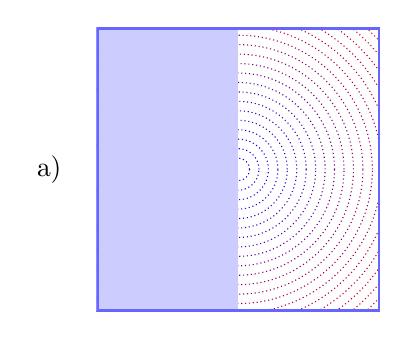
\begin{tikzpicture}[scale=1.2]
            \node[] at (-2, 0) {a)};
            \begin{scope}
                \clip (-1.5, -1.5) rectangle (1.5, 1.5);
                \foreach \cRadius in {1, ..., 22}
                    \pgfmathsetmacro\cColor{\cRadius/22*100}
                    \draw[red!\cColor!blue, densely dotted] (0, 0) circle (0.02+\cRadius*0.1); 
                    
                \fill[blue!20] (-1.5, -1.5) rectangle (0, 1.5);
                \draw[blue!60, ultra thick] (-1.5, -1.5) rectangle (1.5, 1.5);
            \end{scope}
        \end{tikzpicture}
        \qquad
        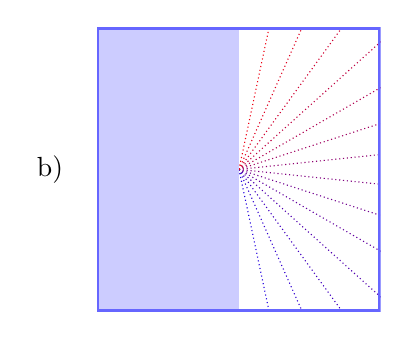
\begin{tikzpicture}[scale=1.2]
            \node[] at (-2, 0) {b)};
            \begin{scope}
                \clip (-1.5, -1.5) rectangle (1.5, 1.5);
                \foreach \cAngle in {1, ..., 16}
                    \pgfmathsetmacro\cColor{\cAngle/16*100}
                    \draw[red!\cColor!blue, densely dotted] (0, 0) -- (\cAngle* 180 / 15 -102:3); 
                \fill[blue!20] (-1.5, -1.5) rectangle (0, 1.5);
                \draw[blue!60, ultra thick] (-1.5, -1.5) rectangle (1.5, 1.5);
            \end{scope}
        \end{tikzpicture}
    \end{center}
    \caption{Schéma représentant l'extraction de caractéristiques à partir de l'espace de Fourier. En a), l'utilisation de cercles concentriques depuis l'origine, schématisé en pointillés ; En b), l'extraction selon une direction.}
    \label{fig:scheme_fourier_features}
\end{figure}\par

La transformée en ondelettes possède divers avantages dont une bonne capacité de localisation, par translation de l'ondelette mère, et la possibilité de prendre en considération plusieurs échelles d'analyse, par homothétie~\cite{Livens1997,Wiltgen2008}. Concernant le choix de l'ondelette mère, celui-ci ne semble pas affecter la qualité des caractéristiques extraites~\cite{Fatemi1996, Livens1997}. Néanmoins, l'un des auteurs préconise le choix d'ondelette symétrique ou anti-symétrique~\cite{Livens1997}. Plusieurs de nos références s'orientant vers des ondelettes de Daubechies ou de Haar, nous privilégierons ces dernières dans nos expériences~\cite{Wiltgen2008,Halimi2017a}. La décomposition en ondelettes sur images se réalise en 3 étapes successives : 
\begin{inlinerate}
    \item de filtrage passe-bas et passe-haut horizontal,
    \item de filtrage passe-bas et passe-haut vertical,
    \item puis une étape de sous-échantillonnage afin de réduire la quantité d'information généré apr ces deux précédentes étapes.
\end{inlinerate} Ce processus est trois temps est schématisé en \Cref{fig:scheme_dwt}. Nous effectuerons la transformée en ondelettes de ce travail à l'aide de la bibliothèque logicielle "PyWavelets"~\cite{lee2006}.\par

\begin{figure}[H]
    \centering
    \includegraphics[width=0.7\textwidth]{contents/chapter_4/resources/scheme_dwt.pdf}
    \caption{Principe de la décomposition en ondelettes appliquée aux images~\cite{Livens1997}. La décomposition est réalisée en trois temps. Un filtrage passe bas (L) et passe haut (H) sont réalisés selon la direction horizontale, puis selon la direction verticale. Enfin, un sous échantillonnage de coefficient 2 est appliqué afin d'obtenir une matrice de même taille que l'image d'origine.}
    \label{fig:scheme_dwt}
\end{figure}\par 

Ainsi, nous réaliserons plusieurs de ces expériences sur base de descripteurs en fréquence. Dans un premier temps, nous tenterons d'étudier l'efficacité des transformations de Fourier et en ondelettes (à l'aide des ondelettes mère de Daubechies et de Haar) sur la séparation des classes. Puis dans un second temps, nous reproduirons la méthode de la littérature employant une combinaison de descripteurs de l'espace de Fourier~\cite{Wiltgen2008}. La \Cref{tab:number_features_frequency} synthétise le nombre associé de caractéristiques extraites par ces diverses méthodes d'extraction fréquentielles.\par

\begin{table}[H]
    \centering
    \begin{tabular}{ll}
        \toprule
        \textbf{Méthode}                        & \textbf{Nombre de caractéristiques}   \\ \hline
        Fourier                                 & 10 / 20 / 30                          \\ \hline
        Ondelettes de Daubechies                & 12                                    \\ \hline
        Ondelettes de Haar                      & 12                                    \\ \hline
        Wiltgen~\cite{Wiltgen2008} - Fourier    & 38 (22+16)                             \\
        \bottomrule
    \end{tabular}
    \caption{Liste des méthodes fréquentielles évaluées dans ce chapitre et leur nombre de caractéristiques extraites associées.}
    \label{tab:number_features_frequency}
\end{table}\par

\subsection{Technique d'apprentissage par transfert de connaissances}
Les techniques d'apprentissage par transfert de connaissances sont un champ d'application relativement récent des techniques d'apprentissage automatique. Le principe est de réutiliser des connaissances précédemment acquises, dans le but de résoudre de nouveau problèmes plus rapidement voire plus efficacement. Pour cela, ce champs vise à proposer des techniques permettant la transposition de connaissance d'une ou plusieurs tâches sources à une tâche cible~\cite{QiangYang2010}.\par

Le phénomène conjoint d'engouement pour les \gls{cnn} et la complexité des architectures récentes pour le traitement des images a accentué les recherches en ce sens. En effet, les techniques d'apprentissage par transfert de connaissance sont une réponse efficace à de nombreuses problématiques autour de l'entraînement des \gls{cnn}, comme : 
\begin{itemize}
    \item les \textbf{contraintes de suffisance de données}, notamment de données convenablement structurées et annotées disponible publiquement,
    \item le \textbf{complexité de l'entraînement}, comprenant le réglage des divers paramètres de ces réseaux (augmentations des données, fonction d'optimisation, \ldots),
    \item et les \textbf{contraintes matérielles nécessaires}, regroupant les aspects matériels dédiés au support de l'entraînement de ces architectures.
\end{itemize}\par

Certains domaines d'application ont vu apparaître de nombreuses bases de données publique, contribuant à résoudre partiellement la contrainte liée aux données. Ces bases ont également pour objectif de permettre de mesurer les performances de système de traitement de l'image, nous retrouvons notamment : 
\begin{inlinerate}
    \item la \textbf{base MNIST}, pour mesurer l'aptitude de systèmes dédiés à la reconnaissance de chiffres manuscrit~\cite{lecun2010},
    \item les \textbf{bases CIFAR10 et CIFAR100}, permettant l'évaluation de systèmes de reconnaissance d'objets sur des image miniatures~\cite{Krizhevsky}, 
    \item et plus récemment, la \textbf{base ImageNet} pour la reconnaissance d'objets sur des images de taille communes~\cite{Deng2008}. 
\end{inlinerate}\par

Actuellement, la base ImageNet est l'une des plus sollicités pour entraîner et évaluer les architectures de \gls{cnn} actuelles. Outre leurs tailles, cette base propose des niveaux d'annotations variées, dont 1000 classes sont proposées. De plus, une très grande diversité d'échantillons est mise à disposition pour chaque classe pour un total de plus de 14 millions d'images. Selon certaines études, ce nombre d'images reste néanmoins sur-dimensionné vis-à-vis du nombre d'éléments nécessaire à l'entraînement de ces réseaux~\cite{Huh2016}.\par

Parallèlement à ce phénomène de mise à disposition de bases de données, sont ouvert publiquement des défis visant à démontrer l'efficacité de chaînes de traitement pour gérer ces données. De nombreuses avancées ont été réalisées sur la base ImageNet, à l'aide d'architectures de \gls{cnn} régulièrement dévoilés et mise à disposition de la communauté. Parmi ces réseaux nous pouvons citer les réseaux AlexNet~\cite{Krizhevsky2012}, GoogLeNet~\cite{Szegedy2015}, VGG~\cite{Simonyan2014}, Inception-V3~\cite{Szegedy2016}, ResNet~\cite{He2016} et Inception-ResNet~\cite{Szegedy2017}, avec respectivement comme précisions 0,54, 0,68, 0,71, 0,76, 0,78, and 0,80 sur la base ImageNet~\cite{Canziani2016}.\par

Néanmoins, la mise à disposition de la communauté de ces bases de données massives et de ces architectures ne permettent de lever les deux verrous liées au contraintes d'entraînement et matérielles de ces réseaux. C'est donc particulièrement le partage de modèles de \gls{cnn} pré-entraînés, couplé aux principes d'apprentissage par transfert de connaissances, qui ont suscités l'intérêt de nombreux travaux dont certains appliqué à de l'imagerie médicale~\cite{Litjens2017}. Ainsi, la majeure partie de ces réseaux pré-entraîné sont obtenus à l'aide de la base ImageNet, bien qu'aucune justification formelle n'ait été fournie à ce propos~\cite{Huh2016}.\par
 
\begin{figure}[H]
    \centering
    \includegraphics[width=\linewidth]{contents/chapter_4/resources/scheme_transfer_learning.pdf}
    \caption{Schéma représentant l'apprentissage par transfert par \gls{cnn}. Le réseau est entraîné sur des données et annotations d'une problématique \textit{source}. Puis, les paramètres de la partie liée à l'extraction de caractéristiques sont conservés et réemployé au sein d'une nouvelle problématique \textit{cible}.}
    \label{fig:scheme_transfer_learning}
\end{figure}\par

L'apprentissage par transfert sur \gls{cnn} se décompose en deux procédés majeurs : 
\begin{inlinerate}
    \item d'une part l'extraction de caractéristiques moins coûteuse en ressources matérielles et temps,
    \item et d'autre part le réglage fin qui nécessite à l'inverse plus de temps et de ressources matérielles. 
\end{inlinerate}
Au sein de cette partie, nous nous focaliserons sur l'extraction de caractéristiques, schématisé en \Cref{fig:scheme_transfer_learning}, afin de limiter les contraintes d'apprentissage. Le principe consiste dans un premier temps à retirer les couches responsables de la classification du problème cible, puisque spécifiques au problème initial. Ces couches sont généralement des couches dites totalement connectées, qui vont pondérer l'importance des zones d'activation jusqu'au classes respectives. Dans un second temps, les couches responsables de l'extraction de caractéristiques sont conservées puis figées, en partant du postulat que ces caractéristiques sont suffisamment variées et adaptées à d'autres problématiques du traitement d'image. Enfin, ces couche sont combinées à de nouvelles couches totalement connectées ou à des modèles de classification~\cite{Litjens2017}.\par 

A cette fin, une première stratégie consiste à aplatir l'information des couches d'extraction par une étape de "Flatten" (littéralement "Applatissement"), transformant celle-ci d'un format de matrice 3D à un vecteur 1D (voir \Cref{fig:scheme_global_pooling} - Gauche). Néanmoins, l'une des problématiques résultantes concerne la dimension spatiale souvent importante de ces caractéristiques extraites. En effet, la dimension spatiale de ces données sera réduite par les couches convolutionelles selon leurs paramètres dépendants de l'architecture choisie. Ainsi, les paramètres de décalage, de pas ou encore de taille du noyau de convolution sont autant de paramètre qui affecterons la dimension spatiale de sortie. Pour pallier à cette information conséquente, des couches dites de "Global pooling" ont été introduites dans la littérature, et consistent à réduire l'information spatiale d'une carte d'activation à une unique valeur (voir \Cref{fig:scheme_global_pooling} - Droite). Les principales fonctions mises à disposition sont la fonction maximum et moyenne, donnant respectivement lieu à des couches de "Global Maximum Pooling" et "Global Average Pooling". D'autres fonctions sont également développées, mais la littérature s'accordera à préférer l'utilisation des couches de "Global Maximum Pooling"~\cite{christlein2019}.\par

\begin{figure}[H]
    \centering
    \includegraphics[width=\linewidth]{contents/chapter_4/resources/scheme_global_pooling.pdf}
    \caption{Schéma représentant l'aplatissement et la réduction d'information par "Global Pooling" au sein de \gls{cnn}. Le réseau est entraîné sur des données sources, généralement plus complètes. Puis, les paramètres de la partie liée à l'extraction de caractéristiques sont conservés et réemployé au sein d'une nouvelle problématique cible.}
    \label{fig:scheme_global_pooling}
\end{figure}\par

Bien que la plupart des travaux en imagerie médicale s'oriente vers l'architecture Inception-V3, son efficacité n'a pas été formellement démontrée au sein des applications médicales. La principale raison la plus probable expliquant le choix de cette architecture est la mise à disposition de ses modèles pré-entraînés par la plupart des librairies de \gls{cnn}~\cite{Litjens2017}. Les différentes expériences que nous mènerons sur l'apprentissage par transfert se focaliseront sur des architectures relativement récentes pré-entraînés sur la base d'image ImageNet et proposés par la bibliothèque "Keras Applications"~\cite{chollet2015a}. Afin de traiter les images dans leur intégralité, nous ne nous baserons que sur des réseaux dont les couches d'extraction de caractéristiques sont purement convolutionnelles et donc indépendante de la taille de l'entrée. Ainsi, nous ne conserverons que quelques architectures de \gls{cnn} représentatives des avancés dans le domaine durant la dernière décennie, dont VGG, Inception-V3, ResNet et Inception-ResNet. L'ensemble des réseaux employés et nombre de paramètres extraits associés sont résumés au sein de la \Cref{tab:number_features_transferlearning}. Finalement, la manipulation des \ac{cnn} est réalisée à haut niveau grâce à la bibliothèque logicielle "Keras"~\cite{chollet2015} et sera couplée à la bibliothèque de bas niveau "Tensorflow"~\cite{tensorflow2015}.\par

\begin{table}[H]
    \centering
    \begin{tabular}{lll}
    \toprule
    \textbf{Architecture}               & Global Pooling   & \textbf{Nombre}    \\ \hline
    \multirow{2}{*}{VGG-16}             & Maximum          & 512                \\ \cline{2-3}
                                        & Moyenne          & 512                \\ \hline
    \multirow{2}{*}{Inception-V3}       & Maximum          & 2048               \\ \cline{2-3}
                                        & Moyenne          & 2048               \\ \hline
    \multirow{2}{*}{ResNet}             & Maximum          & 2048               \\ \cline{2-3}
                                        & Moyenne          & 2048               \\ \hline
    \multirow{2}{*}{Inception-ResNet}   & Maximum          & 1536               \\ \cline{2-3}
                                        & Moyenne          & 1536               \\
    \bottomrule
    \end{tabular}
    \caption{Liste des architecture de \gls{cnn} employés dans ce chapitre et leur nombre de caractéristiques extraites associées.}
    \label{tab:number_features_transferlearning}
\end{table}\par

\subsection{Analyse préliminaire des méthodes d'extraction}
Cette analyse préliminaire de l'information a pour but de montrer l'impact des méthodes d'extraction de caractéristiques précédemment citées sur le jeu de données en notre possession. Nous nous pencherons d'une part sur l'observation de deux images typiques de tissus malin et bénin par l'application des transformations et d'autre part, nous étudierons la capacité de séparation de chacune des méthodes précédentes sur l'ensemble des images.\par

Tout d'abord, il est intéressant de constater en général, la présence de motif plus lisses et moins contrastés au sein des images bénignes que des images malignes. L'application de \gls{glcm} de premier ordre sur nos images typiques est visible sur la \Cref{fig:example_glcm}. Il est possible d'observer une uniformité de cette information quelle que soit la direction observée, allant dans le sens de l'utilisation de la moyenne sur les caractéristiques proposé par Haralick~\cite{Wiltgen2008}. Enfin, cette transformation montre une certaine cohérence des transitions dans les images avec des valeurs présentes en majorité sur la diagonale. Néanmoins, ce phénomène semble plus intense sur l'image bénigne, traduisant des transitions plus douces que sur l'image maligne.\par

\begin{figure}[H]
    \centering
    \includegraphics[width=\linewidth]{contents/chapter_4/resources/example_glcm.pdf}
    \caption{Exemple d'extraction de \gls{glcm} de second ordre sur deux images typique. En haut, un cas d'image bénigne ; En bas, une image pathologique typique de \gls{lm}.}
    \label{fig:example_glcm}
\end{figure}\par

La \Cref{fig:example_fft} met en application la transformée de Fourier centrée sur ces deux même images. L'observation du module de cette transformation permet de constater une information plus présente en intensité sur les basses fréquences que sur les hautes fréquences de l'image bénigne, là où sur l'image maligne cette information au centre forme une tâche plus diffuse. En revanche, à premier abord, la direction ne semble pas apporter d'information pertinente comme suggéré par l'article de Wiltgen~\cite{Wiltgen2008}.\par

\begin{figure}[H]
    \centering
    \includegraphics[width=0.8\linewidth]{contents/chapter_4/resources/example_fft.pdf}
    \caption{Exemple de transformée de Fourier centrée appliquée à deux images typiques, représentation selon le module et la phase. En haut, un cas d'image bénigne ; En bas, une image pathologique typique de \gls{lm}.}
    \label{fig:example_fft}
\end{figure}\par

Enfin, nous terminons l'étude de ces deux exemples par l'application de décomposition en ondelettes. La \Cref{fig:example_wavelet_db4} reflète cette décomposition d'ondelettes de Daubechies tandis que la \Cref{fig:example_wavelet_haar} nous donne un aperçu de cette même méthode par ondelettes de Haar. Nous pouvons constater que les ondelettes de Haar semblent plus propices à isoler les zones de fortes transition que celle de Daubechies. Néanmoins, pour ces deux types d'ondelettes, les décompositions de l'image bénigne semble plus homogènes que celle de l'image maligne. De même, l'extraction des hautes fréquences sur l'axe vertical et horizontal semble plus adaptée que l'extraction combiné de ces deux axes pour l'image maligne.\par

\begin{figure}[H]
    \centering
    \includegraphics[width=\linewidth]{contents/chapter_4/resources/example_wavelet_db4.pdf}
    \caption{Exemple de transformée en ondelettes (Daubechies) appliquée à deux images typiques, à 2, 3 puis 4 niveaux. En haut, un cas d'image bénigne ; En bas, une image pathologique typique de \gls{lm}.}
    \label{fig:example_wavelet_db4}
\end{figure}\par

\begin{figure}[H]
    \centering
    \includegraphics[width=\linewidth]{contents/chapter_4/resources/example_wavelet_haar.pdf}
    \caption{Exemple de transformée en ondelettes (Haar) appliquée à deux images typiques, à 2, 3 puis 4 niveaux. En haut, un cas d'image bénigne ; En bas, une image pathologique typique de \gls{lm}.}
    \label{fig:example_wavelet_haar}
\end{figure}\par

Dans le but d'évaluer la séparation des classes, nous nous aiderons de l'\gls{pca}. En effet, malgré l'extraction de caractéristiques les données en notre possession contiennent un grand nombre de dimensions, rendant le problème difficile à analyser visuellement. De nombreuses techniques de réduction de l'information permettant une meilleure visualisation sont proposé dans la littérature, comme par exemple le T-SNE~\cite{Maaten2008} mais dont le principal inconvénient réside dans le nombre de degrés de liberté proposés. Néanmoins, l'\gls{pca} est une technique communément acceptée à cette fin~\cite{Himberg2001} et possède l'avantage de ne pas être dépendante de ce type de paramètres. Nous faisons également figurer la variance propre à ces deux axes, et pour chaque classes leur centre et leur dispersion sur la base de l'écart type.\par

Ainsi, la \Cref{fig:visualisation_spatial} met en évidence cette technique pour l'ensemble des méthodes d'extraction spatiales. Le premier constat concernant la variance expliquée est que ces deux axes semblent à même de fournir l'intégralité de la variance. Les données extraites à l'aide des techniques d'extraction de premier ordre ne semblent pas optimaux comme nous pouvons le constater sur \Cref{fig:visualisation_spatial}. En effet, les centres de masses et leur dispersion semble assez similaire, notamment pour les données bénignes et malignes. De plus, la séparation des classes ne semble pas marquée dans ces divers schémas d'extraction, et les classes de données vont jusqu'à se chevaucher pour les classes bénignes et saines pour les méthodes employant les caractéristiques d'Haralick. Par ailleurs, la distribution des méthodes employant ces caractéristiques d'Haralick semble similaire, suscitant de faibles différences entre elles.\par

\begin{figure}[H]
    \centering
    \begin{subfigure}{.45\textwidth}
      \includegraphics[width=\textwidth]{contents/chapter_4/resources/visualisation_spatial_FirstOrder.png}
    \end{subfigure}
    \begin{subfigure}{.45\textwidth}
      \includegraphics[width=\textwidth]{contents/chapter_4/resources/visualisation_spatial_Haralick.png}
    \end{subfigure}
    
    \begin{subfigure}{.45\textwidth}
      \includegraphics[width=\textwidth]{contents/chapter_4/resources/visualisation_spatial_HaralickMean.png}
    \end{subfigure}
    \begin{subfigure}{.45\textwidth}
      \includegraphics[width=\textwidth]{contents/chapter_4/resources/visualisation_spatial_WiltgenSpatial.png}
    \end{subfigure}
    
    \caption{Visualisation des caractéristiques obtenues par techniques d'extraction spatiales et projection \gls{pca} sur les deux premières composantes.}
    \label{fig:visualisation_spatial}
\end{figure}\par

La \Cref{fig:visualisation_frequency} permet de mettre en évidence la distribution des données extraites par les méthodes d'extraction fréquentielle. Ainsi, les méthodes basées sur l'extraction de caractéristiques de Fourier semblent posséder une distribution similaire quel que soit le nombre de caractéristiques extraites. De plus, la méthode de Fourier proposé par Wiltgen~\cite{Wiltgen2008}, proposant d'extraire des caractéristiques selon diverses directions, ne semble pas influer cette distribution. Du point de vue des méthodes basées sur le principe d'ondelettes, la séparation des données semble être davantage marquée, et l'impact de l'ondelette mère ne semble pas influer sur la distribution des données et des classes. Pour l'ensemble de ces méthodes, les deux premières composantes de l'\gls{pca} semblent suffisantes à exprimer la quasi-intégralité de la variance.\par

\begin{figure}[H]
    \centering
    \begin{subfigure}{.45\textwidth}
      \includegraphics[width=\textwidth]{contents/chapter_4/resources/visualisation_frequency_Fourier10.png}
    \end{subfigure}
    \begin{subfigure}{.45\textwidth}
      \includegraphics[width=\textwidth]{contents/chapter_4/resources/visualisation_frequency_Fourier20.png}
    \end{subfigure}
    
    \begin{subfigure}{.45\textwidth}
      \includegraphics[width=\textwidth]{contents/chapter_4/resources/visualisation_frequency_Fourier30.png}
    \end{subfigure}
    \begin{subfigure}{.45\textwidth}
      \includegraphics[width=\textwidth]{contents/chapter_4/resources/visualisation_frequency_WiltgenFourier.png}
    \end{subfigure}
    
    \begin{subfigure}{.45\textwidth}
      \includegraphics[width=\textwidth]{contents/chapter_4/resources/visualisation_frequency_Haar.png}
    \end{subfigure}    
    \begin{subfigure}{.45\textwidth}
      \includegraphics[width=\textwidth]{contents/chapter_4/resources/visualisation_frequency_Daubechies.png}
    \end{subfigure}
    
    \caption{Visualisation des caractéristiques obtenues par techniques d'extraction fréquentielles et projection \gls{pca} sur les deux premières composantes.}
    \label{fig:visualisation_frequency}
\end{figure}\par

Pour finir, la \Cref{fig:visualisation_transfer} recense les projections par \gls{pca} de l'ensemble des méthodes d'extraction basée sur des architecture de \gls{cnn} pre entrainées, catégorisées sous le terme de transfert par apprentissage. Une différence notable est à remarquer entre les architectures utilisant une couche de global pooling moyen et celle utilisant une couche de global pooling maximum. En effet, la séparation entre classes est marquée de manière plus importante lorsque qu'une couche de global pooling moyen est employé. En addition, cette séparation semble être plus prononcée sur les architectures InceptionV3 et ResNet. Enfin, nous pouvons noter par ces méthodes, que la variance exprimée sur les deux premières composantes n'est que de 20\% à 40\%. Ce dernier constat s'explique par la grande quantité d'information initialement proposé par ces architectures, soit entre 512 et 2048 caractéristiques extraites en comparaison des dizaine d'entre elles extraites par les méthodes manuelles.\par

\begin{figure}[H]
    \centering
    \begin{subfigure}{.45\textwidth}
      \includegraphics[width=\textwidth]{contents/chapter_4/resources/visualisation_transfer_VGG16Avg.png}
    \end{subfigure}
    \begin{subfigure}{.45\textwidth}
      \includegraphics[width=\textwidth]{contents/chapter_4/resources/visualisation_transfer_VGG16Max.png}
    \end{subfigure}
    
    \begin{subfigure}{.45\textwidth}
      \includegraphics[width=\textwidth]{contents/chapter_4/resources/visualisation_transfer_InceptionV3Avg.png}
    \end{subfigure}
    \begin{subfigure}{.45\textwidth}
      \includegraphics[width=\textwidth]{contents/chapter_4/resources/visualisation_transfer_InceptionV3Max.png}
    \end{subfigure}
    
    \begin{subfigure}{.45\textwidth}
      \includegraphics[width=\textwidth]{contents/chapter_4/resources/visualisation_transfer_ResNetAvg.png}
    \end{subfigure}
    \begin{subfigure}{.45\textwidth}
      \includegraphics[width=\textwidth]{contents/chapter_4/resources/visualisation_transfer_ResNetMax.png}
    \end{subfigure}
    
    \begin{subfigure}{.45\textwidth}
      \includegraphics[width=\textwidth]{contents/chapter_4/resources/visualisation_transfer_InceptionResNetAvg.png}
    \end{subfigure}
    \begin{subfigure}{.45\textwidth}
      \includegraphics[width=\textwidth]{contents/chapter_4/resources/visualisation_transfer_InceptionResNetMax.png}
    \end{subfigure}
    
    \caption{Visualisation des caractéristiques obtenues par techniques d'extraction basées sur des réseaux de type \gls{cnn} pré-entraînés sur la base ImageNet et projection \gls{pca} sur les deux premières composantes.}
    \label{fig:visualisation_transfer}
\end{figure}\par

\clearpage


%%%%%%%%%%%%%%%%%%%%%%%%%%%%%%%%%% 
%%%%%%%%%%%%%%%%% PRE TRAITEMENTS
\section{Pré-traitements de caractéristiques}
Cette partie dédiée au pré-traitement de caractéristiques, se consacre à l'ensemble des transformations opérées après extraction de l'information par le biais des techniques évoquées en \Cref{chap:feature_extraction}. Nous aborderons au sein de cette section les diverses solutions à notre disposition pouvant parfaire la classification de notre problématique. En effet, de nombreuses contraintes peuvent affecter le bon déroulement de la classification :
\begin{itemize}
    \item un déséquilibre au sein des annotations des divers types de tissus a séparé bien que celui-ci ait été minimisée,
    \item un nombre de caractéristiques trop important conduisant à du sur-apprentissage ou des difficultés à séparer le problème (voir l'extraction de caractéristiques par \gls{cnn}),
    \item ou encore une information non consistante.
\end{itemize}\par

Ainsi, cette partie tentera de répondre à ces questions à l'aide de différents domaines d'étude visant à corriger tout ou partie de ces éléments et nous les aborderons d'un point de vue logique en termes de processus de classification. Ainsi et dans un premier temps, nous discuterons de la \textbf{normalisation} des caractéristiques et de son intérêt au sein de processus de classification. Dans un second temps, nous traiterons des techniques de \textbf{réduction de l'information} et proposerons des solutions notamment dans le cadre de l'extraction de caractéristiques par \gls{cnn}. Finalement, nous aborderons le \textbf{balancement de données} et les principales stratégies mises à disposition.

\subsection{Réduction de dimensions}
Dans le domaine de l'apprentissage automatique, la réduction de dimension est une technique qui permet de diminuer le nombre de dimensions afin de rendre un problème moins complexe, tout en conservant une information suffisante à la résolution du problème. Également, elle est un moyen de se prévenir du "Fléau de la dimension", phénomène qui met en perspective d'une part la croissance exponentielle de l'ajout de nouvelles dimensions à la dilution des divers échantillons dans cet espace. Ce dilemme a pour principales conséquences d'augmenter la complexité d'un problème, la durée nécessaire à sa résolution mais également d'engendrer des risques de sur-apprentissage.\par

Les caractéristiques extraites par méthode spatiales et fréquentielles étant assez restreintes (respectivement de 14 à 56 variables et, de 10 à 39 variables), nous n'étudierons pas leur impact sur ces méthodes. En revanche, le nombre des caractéristiques extraite par méthode de transfert de connaissance est important et varient de 512 à 2048 variables. Nous évaluerons l'impact de certaines d'entre elles sur ces cas particuliers.\par

A cette fin, deux catégories de méthodes cohabitent : d'une part les méthodes de sélection de caractéristiques qui réduisent l'espace en décimant certaines dimensions jugées non pertinente à la résolution du problème ; d'autre part les méthodes par projection ou transformation de l'espace existant qui réduisent et modifient les valeurs existantes. Dans la mesure où nous emploierons cette technique dans le cadre de l'apprentissage par transfert de connaissance, notre investigation ne portera que sur cette seconde catégorie de méthodes. En effet, les méthodes par sélection de caractéristiques ne nous semblent pas pertinente dans le cadre de caractéristiques auto déterminées par des réseaux profonds.\par

L'\gls{pca} est l'une de ces techniques, dont l'idée majeure est de retirer l'information redondante pour ne conserver que l'information de variance, supposée contenir l'information. Cette méthode cherche ainsi à identifier les axes selon lesquels la variation des données est maximisée. Il sera ensuite nécessaire de déterminer un nombre d'axes suffisant à séparer le problème (réduction du nombre de caractéristiques). Plutôt que de choisir ce nombre arbitraire, la littérature préfère retenir des seuils pertinents de cette variance, les plus communs sont 95\%, 97.5\% et 99\%.\par

Le \gls{lda} est une seconde technique employée à une fin de réduction de l'information, pour laquelle nous recherchons des axes de projection qui maximisent la variance inter-groupe. Pour comparaison, la variance est le résultat de la somme de la variance intra-groupe et inter-groupe. De la même manière, nous retiendrons des seuils similaires à ceux de l'\gls{pca} soit 95\%, 97.5\% et 99\%.\par

La \Cref{tab:summary_reduction_methods} permet de résumer ces méthodes et paramétrage associés que nous évaluerons.\par 

\begin{table}[H]
    \centering
    \begin{tabular*}{0.6\linewidth}{lll}
        \toprule
        \textbf{Méthode}       & \textbf{Paramètre}                 & \textbf{Valeurs}                      \\ \midrule
        \gls{pca}              & \multirow{2}{*}{Variance expliquée}& \multirow{2}{*}{[0.95, 0.975, 0.99]}  \\ \cline{1-1}
        \gls{lda}              &                                    &                                       \\ 
        \bottomrule
    \end{tabular*}
    \caption{Liste des méthodes de réduction employées et leurs paramètres associés.}
    \label{tab:summary_reduction_methods}
\end{table}\par

\subsection{Normalisation de caractéristiques}
\label{subsec:features_normalisation}
Selon le domaine d'étude visée, la normalisation de caractéristiques peut être l'une des étapes cruciales quant au bon déroulement de ce processus de classification. Notre recherche a été amenée à considérer cet aspect suite à la dégradation des résultats d'un travail proche de notre thématique portant sur la classification d'image de dermatoscopie~\cite{Celebi2007}.\par

Il est communément admis que des méthodes tels que les \gls{knn} dont le principe repose sur des critères de distances, peuvent être fortement affectés par des caractéristiques non normalisées. Pour d'autres méthodes de classification, cette normalisation des caractéristiques fait davantage appel à un bon sens vis-à-vis de leur principe de fonctionnement. Nous noterons le retour de certains travaux sur la dégradation des performances sur les \gls{svm}~\cite{Juszczak2002} mais également les réseaux de neurones~\cite{Celebi2007}.\par

Diverses méthodes ont ainsi été proposées afin de remédier à ces défauts de distribution de l'information. L'un de ces travaux propose de réduire l'erreur de classification de modèles \gls{svm} par l'apport de normalisations tenant compte de la variance, du maximum ou encore conjointement du minimum et du maximum~\cite{Juszczak2002}. Le travail mené par Celebi et al.~\cite{Celebi2007} propose une normalisation des caractéristiques à l'aide de la "Cote Z" ou "Standard score", c'est à dire par soustraction de la moyenne au sein d'un même groupe de caractéristiques puis par division de l'écart type de ce même groupe.\par

Afin de couvrir au mieux cette problématique de la normalisation, nous l'aborderons à l'aide des deux méthodes majeure de ces deux précédentes études, dont l'\Cref{eq:scaling_methods} reprend les expressions sous forme mathématique. Ainsi, nous envisagerons l'utilisation de :
\begin{itemize}
    \item la normalisation par "Mininimum et Maximum"~\cite{Juszczak2002},
    \item et de la normalisation "Standard" ou "Cote Z"~\cite{Celebi2007}.
\end{itemize}\par

\begin{equation} 
    \label{eq:scaling_methods}
    \begin{split}
    &MinMax=\frac{X-min(X)}{max(X)-min(X)}  \\
    &Standard=\frac{X-\mu{}}{\sigma}	    
    \end{split}
\end{equation}

\subsection{Balancement de données}
L'une des problématiques associées de manière récurrente à l'apprentissage sur des données réelles est celle de la répartition homogène des annotations, en opposition aux domaines impliquant des données synthétiques pouvant provenir de modèles génératifs par exemple. Ces déséquilibres d'annotations sont qualifiés sous le terme anglophone de "class imbalance"~\cite{Prati2009, He2009}.\par

Ces déséquilibres sont propres à de nombreux domaines d'applications, mais touchent essentiellement des champs d'activités dans lesquels la tâche visée correspond à la détection d'événements isolés au sein d'une population, comme par exemple : 
\begin{inlinerate}
    \item les comportements déviants (fraude bancaire~\cite{Phua2004}),
    \item le respect de critère de qualité (vérification de pièces industrielles~\cite{Wu2018}),
    \item ou encore d'anormalités clinique (cancers ou d'autres pathologies cliniques~\cite{Celebi2007}).
\end{inlinerate}\par

Certains choix peuvent permettre de limiter l'impact d'un déséquilibre d'annotations. Ainsi, la sélection d'un métrique adéquate peut permettre de limiter la dépendance au données : la substitution de la précision par des mesures telles que l'\gls{auc}~\cite{Celebi2007} ou le \fscore{} sont des solutions pertinentes dans de telles situations. Néanmoins, la plupart des modèles de classification échoueront à classifier convenablement les données dans des situations de forts déséquilibres. Ces modèles préférerons prédire constamment la classe majoritaire, pour minimiser le coût de l'erreur~\cite{Huang2013}. Dans le cadre de modèles basés sur des arbres de décision, la stratégie générale propose de déterminer les critères majeurs de séparation par partitionnement successif des données. Ce partitionnement conduit inéluctablement à un affaiblissement des classes minoritaires~\cite{He2009}. Deux catégories d'approches coexistent pour solutionner ces déséquilibres~\cite{Huang2013}, d'une part les approches par augmentation ou décimations des diverses catégories d'annotation, et d'autres part les approches algorithmiques consistent à pondérer la valeur des annotations afin de prendre en considération le déséquilibre de l'information~\cite{Ting2002,He2009,Thai2010}.\par

En premier lieu, des approches par correction des données simples, proposes diverses solutions pour palier à ces déséquilibres de classes~\cite{Prati2009, He2009}. Une première catégorie de ces méthodes consiste à \textbf{sous-échantillonner} les données jusqu'à obtenir une égalité entre les classes. Son principe le plus simple est celui du "Sous-échantillonnage aléatoire" consistant à décimer de manière aléatoire les données des classes majoritaires afin d'égaler les échantillons de la classe minoritaire. A l'inverse, une autre catégorie consiste à \textbf{sur-échantillonner} les données possédées afin d'obtenir à nouveau une égalité entre classes. Le principe le plus simples est celui du "Sur-échantillonnage aléatoire" consistant à dupliquer aléatoirement les échantillons des classes minoritaires afin d'égaler le nombre d'élément de la classe majoritaire. Le schéma en \Cref{fig:scheme_data_balancing} reprendre l'idée de ces deux principes.\par

En second lieu, des approches par correction des données plus avancées ont été proposées. De manière non exhaustive nous proposerons l'une d'entre elle pour chaque catégorie :
\begin{itemize}
    \item par \textbf{sous-échantillonnage} : cette catégorie consiste à décimer le nombre d'échantillons à celle de la classe minoritaire. Nous considérerons une décimation des échantillons aléatoire pour cette catégorie.
    \item par \textbf{sur-échantillonnage} : cette catégorie consiste à augmenter les éléments des classes minoritaires. Nous considérerons une duplication aléatoire de ces éléments.
    \item par \textbf{combinaison} : cette catégorie consiste à mêler des méthodes propres aux deux précédentes catégories. L'utilisation de méthode \gls{smote}~\cite{Chawla2002}  est alors réalisé dans un premier temps pour générer de manière synthétique de nouveaux éléments, puis la méthode \gls{tl}~\cite{Tomek1976} ou \gls{enn} est utilisée pour enlever les incohérences des éléments originaux ou synthétiques.
\end{itemize}\par

\begin{figure}[H]
    \centering
    \includegraphics[width=\linewidth]{contents/chapter_4/resources/scheme_data_balancing.pdf}
    \caption{Schéma des deux stratégies principales de balancement de données. A gauche, la stratégie de sous-échantillonnage, dans laquelle des éléments sont aléatoirement choisis jusqu'à réduire l'ensemble des classes au nombre d'éléments de la classe minoritaire ; A droite, la stratégie de sur-échantillonnage, dans laquelle les éléments des classes minoritaires sont dupliqués aléatoirement. }
    \label{fig:scheme_data_balancing}
\end{figure}\par

En opposition à ces méthodes dédiées, les approches par pondération des échantillons consistent à gérer le déséquilibre des annotations en appliquant des poids d'importance différente selon la provenance échantillon lors de l'apprentissage du modèle. Nous considérerons ce choix par défaut, puisqu'il permet de contrer de manière assez intuitive ces

Dans l'optique de récapituler cette partie, les méthodes utilisées dans le but de corriger le déséquilibre des données sont référencée dans la \Cref{tab:summary_balancement_methods}. Afin de traiter au mieux cette tâche, la balancement de données par ses différentes stratégies évoquée sera réalisé avec l'aide de la librairie logicielle "Imbalanced-learn"~\cite{Lemaitre2017}. La correction par algorithme, plus précisément pondération, sera réalisé avec l'aide de la bibliothèque "Scikit-learn"~\cite{pedregosa2011}.\par

\begin{table}[H]
    \centering
    \begin{tabular*}{0.6\linewidth}{l@{\extracolsep{\fill}}l}
        \toprule
        \textbf{Catégorie}                  & \textbf{Méthode}      \\ \hline
        Sous-échantillonnage                 & Aléatoire             \\ \hline
        Sur-échantillonnage                  & Aléatoire             \\ \hline
        \multirow{2}{*}{Combinaison}        & SMOTE + Tomek         \\ \cline{2-2}
                                            & SMOTE + EN            \\
        \bottomrule
    \end{tabular*}
    \caption{Liste des diverses méthodes de balancement mises en œuvre pour corriger les déséquilibre de données.}
    \label{tab:summary_balancement_methods}
\end{table}\par

\section{Méthodes de prédiction}
Afin d'œuvrer à la séparation des échantillons en notre possession sur la base de leurs caractéristiques, nous aurons recours à divers modèles de classification, dont nous évaluerons les performances de classification. En effet, bien que les avantages et inconvénients de la plupart d'entre eux aient été évoqués au sein de la \Cref{sec:models_settings}, nous n'avons pas de contraintes de rapidité lors de la phase d'apprentissage ou de prédiction. Seules les performances de classifications seront mesurées dans ce travail.\par

\begin{table}[H]
    \centering
    \begin{tabular}{cll}
        \toprule
        \textbf{Modèle}                                 & \textbf{Hyperparamètres}  & \textbf{Valeurs}                          \\ \midrule
        \multirow{4}{*}{\gls{cart}}                     & Profondeur maximum        & [3, $\infty$]                             \\ \cmidrule{2-3} 
                                                        & Critère de qualité        & [Gini, Entropie]                          \\ \cmidrule{2-3}   
                                                        & Caractéristiques maximum  & [1, 2, 3, 4, 5, 6, 7, 8, 9]               \\ \cmidrule{2-3}   
                                                        & Échantillons minimum      & [1, 2, 3, 4, 5, 6, 7, 8, 9]               \\ \midrule 
        \multirow{4}{*}{\gls{rf}}                       & Profondeur maximum        & [3, $\infty$]                             \\ \cmidrule{2-3} 
                                                        & Critère de qualité        & [Gini, Entropie]                          \\ \cmidrule{2-3}   
                                                        & Caractéristiques maximum  & [1, 2, 3, 4, 5, 6, 7, 8, 9]               \\ \cmidrule{2-3}   
                                                        & Échantillons minimum      & [1, 2, 3, 4, 5, 6, 7, 8, 9]               \\ \midrule 
        \multirow{4}{*}{\gls{gb}}                       & Profondeur maximum        & [3, $\infty$]                             \\ \cmidrule{2-3}
                                                        & Critère                   & [MSE, MAE]                                \\ \cmidrule{2-3} 
                                                        & Caractéristiques maximum  & [1, 2, 3, 4, 5, 6, 7, 8, 9]               \\ \cmidrule{2-3}   
                                                        & Échantillons minimum      & [1, 2, 3, 4, 5, 6, 7, 8, 9]               \\ \midrule 
        \gls{svm} - Noyau linéaire                      & C                         & [0.001, 0.01, 0.1, 1, 10, 100, 1000]      \\ \midrule
        \multirow{2}{*}{\gls{svm} - Noyau RBF}          & C                         & [0.001, 0.01, 0.1, 1, 10, 100, 1000]      \\ \cmidrule{2-3}   
                                                        & Gamma                     & [0.001, 0.01, 0.1, 1, 10, 100, 1000]      \\ \midrule 
        \multirow{5}{*}{\gls{mlp}}                      & Couche cachées            & [(20,), (20,20,), (20,20,20,)]            \\ \cmidrule{2-3}
                                                        & Activation                & [Tanh, ReLu]                              \\ \cmidrule{2-3}
                                                        & Solveur                   & [SGD, Adam]                               \\ \cmidrule{2-3}
                                                        & Alpha                     & [0.001, 0.01, 0.1, 1, 10, 100, 1000]      \\ \cmidrule{2-3}
                                                        & Taux d'apprentissage      & [Constant, Adaptatif]                     \\ \bottomrule 
    \end{tabular} 
    \caption{Table recensant l'ensemble des modèles de classification et leurs hyperparamètres évalués lors des expériences que nous mènerons.}
    \label{tab:image_classification_models_hyperparameters}
\end{table}\par

Dans un premier temps, nous évaluerons nos données à l'aide de \gls{cart} dont l'utilité a été démontré par l'un de nos travaux de référence ~\cite{Wiltgen2008}. Néanmoins, ces modèles tendent au sur-apprentissage dans des contextes où les dimensions sont nombreuses, ainsi nous évaluerons de manière complémentaires les \gls{rf}~\cite{Breiman2001} et les \gls{gb} plus aptes à gérer cet aspect. Dans un second temps, nous envisageons les modèles \gls{svm} employés dans de nombreux contextes de classification~\cite{Smach2008a}, mais également de classification de lésion de la peau~\cite{Celebi2007}. Enfin, nous envisagerons la piste des \gls{mlp} afin de d'évaluer notre problématique de manière non linéaire.\par

Afin d'évaluer au mieux chacun de ces modèles, nous affinerons les hyperparamètres majeurs de chacun de ces modèles. Il sera bien entendu nécessaire de faire des compromis dans le choix de ces valeurs, et opterons pour celles les plus couramment utilisées. L'ensemble des modèles de classification et de leurs hyperparamètres et valeurs associés sont recensés sur la \Cref{tab:image_classification_models_hyperparameters}.\par

\section{Processus et métriques}
Pour réaliser l'évaluation, nous emploierons une validation croisée imbriquée déjà discuté sur le \Cref{sec:models_settings}. Le choix de cette structure de validation a été déterminé car moins sujet au biais~\cite{Cawley2010}. Nous opterons pour des valeurs de quatre lots pour l'évaluation et de deux lots pour la validation, arbitrairement choisies mais représentant un bon compromis vis-à-vis de nos expériences. Ces répartitions sous forme de lot de nos données est visible sur la \Cref{fig:visualisation_folds}.\par

\begin{figure}[H]
    \centering
    \includegraphics[width=0.7\linewidth]{contents/chapter_4/resources/visualisation_folds.png}
    \caption{Visualisation des divers lots d'évaluation utilisés pour l'évaluation des processus de classification.}
    \label{fig:visualisation_folds}
\end{figure}\par

Afin de régler les hyperparamètres et d'évaluer les performances des divers modèles, nous opterons pour un métrique de type \fscore{} également discuté durant le \Cref{sec:models_settings}. En effet, cette métrique est robuste face à des déséquilibres d'annotations, et représente conjointement sous une unique mesure la précision ainsi que le rappel. Son expression est binaire, il sera ainsi calculé pour chaque classe dont nous pondérerons la valeur par le ratio du nombre de d'échantillons disponibles pour chacune d'entre elles.\par

Ces expériences seront menées en plusieurs étapes successives, et nous débuterons par l'évaluation de l'ensemble des méthodes d'extraction de caractéristiques conjointement à la normalisation de l'information selon le Minimum/Maximum et Standard. Aucun de ces tests ne sera mené sur les caractéristiques brutes, les modèles ne convergeant pas dans un temps raisonnable selon le modèle employé.\par

Dans une seconde phase, nous mesurerons l'impact de la réduction de dimension sur les techniques de transfert de connaissance avant de procéder à leur classification. Contrairement aux recommandations de la librairie~\textsuperscript{\ref{footnote:exemple_pca_scaling}}, nous opterons pour un schéma de type réduction de l'information puis de normalisation de caractéristiques avant classification. En effet, les caractéristiques issues de réseaux convolutionnels possèdent une distribution de valeurs consistantes, et n'affectent pas de manière significative les techniques de réduction de dimensions. En revanche, la réduction d'information par techniques de projection peut affecter la consistance de cette distribution des valeurs. Ce phénomène a notamment été observé sur un lot de 500 données choisies arbitrairement, et présentée sur la \Cref{fig:visualisation_scaling_reduction}.\par

Pour finir ces expériences, nous finirons par mesurer l'impact du balancement des données sur les résultats de classification et évaluerons l'utilité des techniques qui visent à corriger ce déséquilibre.\par

Les choix que nous réaliserons entre ces diverses étapes se baseront sur les résultats à trois classes dans la mesure où ces scores seront représentatifs de la capacité à caractériser la problématique dans son ensemble. Néanmoins dans la dernière partie de cette analyse, nous considérerons les résultats de la détection des images malignes, principal objectif visé par ce travail.\par

\addtocounter{footnote}{1}
\footnotetext[\thefootnote]{Source : Scikit-learn - \href{https://scikit-learn.org/stable/auto_examples/preprocessing/plot_scaling_importance.html}{"Importance of Feature Scaling"}. \label{footnote:exemple_pca_scaling}}
 
\begin{figure}[H]
    \centering
    \includegraphics[width=\linewidth]{contents/chapter_4/resources/visualisation_scaling_PCA.pdf}
    \includegraphics[width=\linewidth]{contents/chapter_4/resources/visualisation_scaling_LDA.pdf}
    \caption{Visualisation de l'influence de la réduction des dimensions appliquée au deux premières composantes principales, sur un échantillon constitué arbitrairement de 500 éléments de nos données. En haut, technique de réduction basée sur le \gls{pca} ; En bas, technique de réduction basée sur le \gls{lda}. A gauche, un processus procédant à la réduction puis à la normalisation ; A droite, un processus procédant à la normalisation puis à la réduction.}
    \label{fig:visualisation_scaling_reduction}
\end{figure}\par

\clearpage

\section{Résultats}
Les premières expérimentations menées sur les techniques d'extraction de caractéristiques associés aux techniques de normalisation nous permettent d'isoler celles d'entre elles jugées comme les plus pertinentes. Dans un premier temps du point de vue des techniques d'extraction spatial, nous obtenons un score maximal pour les caractéristiques proposé par Haralick non moyennés de 0,64 associés un écart-type de 0,07. Ce score est maximisé par l'utilisation par l'utilisation conjointe d'un modèle \gls{svm} avec noyau RBF et d'une normalisation par Minimum/Maximum. Dans un second temps du point de vue des techniques fréquentielles, le score de classification à trois classes est rendu maximal par l'utilisation de l'extraction en ondelettes de Daubechies par l'obtention d'un score de 0,67 associé à un écart type de 0,06. Ce score est maximisé par l'utilisation par l'utilisation conjointe d'un modèle \gls{svm} avec noyau linéaire ou RBF et d'une normalisation par Minimum/Maximum ou Standard. Enfin, par l'utilisation de diverses architectures de \gls{cnn}, nous parvenons à obtenir un score de de 0,77 associé à un écart type de 0,04 sur l'architecture ResNet-50 combinée à une couche de pooling moyen. Ce score est maximisé à l'aide d'un modèle \gls{svm} avec noyau linéaire et de la normalisation Minimum/Maximum. L'ensemble des résultats liées à cette première expérience sont visibles sur la \Cref{fig:results_image_classification} et sont détaillés en annexe.\par

\begin{figure}[H]
    \centering
    
    \begin{subfigure}{\textwidth}
      \includegraphics[width=\textwidth]{contents/chapter_4/resources/results_image_classification_mms.pdf}
    \end{subfigure}
    
    \begin{subfigure}{\textwidth}
      \includegraphics[width=\textwidth]{contents/chapter_4/resources/results_image_classification_ss.pdf}
    \end{subfigure}
    
    \caption{Résultats issues de la classification par les diverses techniques d'extraction et, par les modèles de classification mentionnés en couleur. En haut, les résultats provenant de la normalisation par Minimum/Maximum ; En bas, les résultats provenant de la normalisation par score Standard. A gauche, la représentation basée sur les valeurs moyennes ; A droite, la représentation tenant compte de l'écart-type.}
    \label{fig:results_image_classification}
\end{figure}\par

Le second volet de ces expérimentations vise à mesurer l'impact de la réduction d'informations des techniques d'apprentissage par transfert. En effet, la grande quantité d'information issue de ces techniques peut provoquer une dégradation des performances de classification, et nous souhaitons vérifier cette hypothèse par cette expérience. Seules les architectures précédemment évoquées couplées à une couche de global pooling moyen seront évaluées, leurs performances ayant été significativement supérieures à celle ayant un global pooling maximum. D'une part, la technique de réduction basée sur l'\gls{pca} a permis d'obtenir un score maximal de 0,76 et un écart-type plus restreint de 0,03 lorsque la variance cumulée est de 99\%. Ce score est obtenu avec l'utilisation de l'architecture ResNet-50 avec un pooling moyen, d'une normalisation par Minimum/Maximum et d'un modèle \gls{svm} linéaire. D'autre part, la technique de réduction basée sur le \gls{lda} nous permet de maximiser le score à une valeur de de 0,73 et un écart-type de 0,05 à partir d'une valeur de variance cumulée de 95\%. Ces valeurs sont obtenues par l'utilisation de l'architecture VGG-16 avec un pooling moyen, d'une normalisation Standard et d'un modèle \gls{svm} linéaire. L'ensemble des résultats de ce volet de l'expérience ont été reportés sur la \Cref{fig:results_image_classification_reduction}.\par

\begin{figure}[H]
    \centering
    
    \begin{subfigure}{\textwidth}
      \includegraphics[width=\textwidth]{contents/chapter_4/resources/results_image_classification_reduction_mms.pdf}
    \end{subfigure}
    
    \begin{subfigure}{\textwidth}
      \includegraphics[width=\textwidth]{contents/chapter_4/resources/results_image_classification_reduction_ss.pdf}
    \end{subfigure}
    
    \caption{Résultats issues de la classification par l'utilisation de techniques de réduction combinés aux techniques d'extraction par transfert et, par les modèles de classification mentionnés en couleur. Les tracés de couleurs représentent les divers modèles évalués au cours de l'expérience. En haut, les résultats provenant de la normalisation par Minimum/Maximum ; En bas, les résultats provenant de la normalisation par score Standard. A gauche, la représentation basée sur les valeurs moyennes ; A droite, la représentation tenant compte de l'écart-type.}
    \label{fig:results_image_classification_reduction}
\end{figure}\par

La dernière partie de notre expérimentation vise à étudier l'impact de l'équilibrage des données sur la qualité des résultats de classification. Pour cela, les méthodes les plus performantes précédemment évoquées sont employées à cet usage. Ainsi, sur l'ensemble des méthodes évaluées la méthode par transfert, qui pour rappel emploie une architecture ResNet-50 avec un global pooling moyen et une normalisation Minimum/Maximum associée à un modèle \gls{svm} linéaire, atteint un score à trois classes de 0,77 et un écart type de 0,04. Ce score est obtenu avec l'utilisation d'une pondération dans le but de compenser le déséquilibre de données.\par

\begin{table}[H]
    \begin{tabular}{lllllll}
        \toprule
                    & Aucune    & Pond.             & Sur-éch. & Sous-éch. & SMOTE+ENN & SMOTE+Tomek\\ \hline
        Spatial     & 0.55±0.15 & 0.61±0.09         & 0.54±0.15& 0.58±0.11 & 0.60±0.09 & 0.56±0.16  \\
        Fréquentiel & 0.59±0.13 & 0.67±0.06         & 0.55±0.21& 0.58±0.17 & 0.61±0.12 & 0.64±0.10  \\
        \rowcolor[HTML]{E7E6E6}
        Transfert   & 0.71±0.08 & \textbf{0.77±0.04}& 0.74±0.07& 0.72±0.05 & 0.74±0.05 & 0.74±0.05  \\
        Réduction   & 0.71±0.09 & 0.76±0.03         & 0.74±0.06& 0.73±0.04 & 0.73±0.04 & 0.73±0.06  \\
        \bottomrule
    \end{tabular}
    \caption{Résultats à trois classes issus de l'expérience mêlant les méthodes les plus performantes associée aux méthodes de balancement de données évoquées.}
    \label{tab:results_balancement_multi}
\end{table}\par

Du point de vue de la séparation des tissus malins du reste des tissus, la méthode basée sur l'apprentissage par transfert par l'utilisation d'une architecture ResNet-50 avec un global pooling moyen et une normalisation Minimum/Maximum associée à un modèle \gls{svm} linéaire, reste la plus performante avec un score de 0,82 et un très faible écart-type de 0,01.\par

\begin{table}[H]
    \begin{tabular}{lllllll}
        \toprule
                    & Aucune    & Pond.             & Sur-éch.  & Sous-éch. & SMOTE+ENN & SMOTE+Tomek\\ \hline
        Spatial     & 0.65±0.11 & 0.63±0.07         & 0.64±0.10 & 0.64±0.08 & 0.63±0.09 & 0.59±0.27  \\
        Fréquentiel & 0.70±0.09 & 0.68±0.03         & 0.66±0.09 & 0.66±0.09 & 0.61±0.22 & 0.66±0.09  \\
        \rowcolor[HTML]{E7E6E6} 
        Transfert   & 0.81±0.04 & \textbf{0.82±0.02}& 0.81±0.03 & 0.79±0.01 & 0.80±0.02 & 0.82±0.03  \\
        Réduction   & 0.81±0.03 & 0.81±0.01         & 0.81±0.03 & 0.79±0.03 & 0.80±0.01 & 0.81±0.03  \\
        \bottomrule 
    \end{tabular}
    \caption{Résultats de la détection de tissus malin issus de l'expérience mêlant les méthodes les plus performantes associée aux méthodes de balancement de données évoquées.}
    \label{tab:results_balancement_malignant}
\end{table}\par

Enfin, une les courbes \gls{roc} nous permettent d'appréhender les performances de prédiction de ce système. Ainsi, les performances propre à l'ensemble de la base d'images annotés sont homogènes par cette technique avec des scores \gls{auc} compris entre 0,87 et 0,90. Néanmoins, une analyse \gls{roc} des lésions \gls{lm} et \gls{lmm} permet de mettre en avant des performances moins homogènes entre les diverses classes pouvant montrer des difficultés de cette techniques à séparer les tissus de ces lésions, les score \gls{auc} variant entre 0,79 et 0,92. Ces éléments sont visibles sur la \Cref{fig:results_image_classification_roc}.\par

\begin{figure}[H]
    \centering
    \includegraphics[width=\textwidth]{contents/chapter_4/resources/results_image_classification_roc.pdf}
    \caption{Courbes \gls{roc} et scores \gls{auc} associés aux courbes. A gauche, courbes associées à l'ensemble des lésions d'étude ; A droite, courbes associées aux seules cas pathologiques de \gls{lm}/\gls{lmm}.}
    \label{fig:results_image_classification_roc}
\end{figure}\par

\section{Discussion}
A la suite des précédents résultats, il nous est possible dans un premier temps de formuler divers constats pour donner suite à la mise en pratique des diverses méthodes d'extraction de caractéristiques. La première d'entre elle sur les caractéristiques spatiales, met en avant l'utilité de la méthode d'Haralick sur ces données de \gls{rcm}, mais pour lesquelles l'ajout de mesures de premier ordre ne semble pas ou peu impacter le résultat. La seconde d'entre elle concerne les caractéristiques fréquentielles, et sur l'utilité de l'extraction en ondelettes comparée aux caractéristiques extraites à l'aide de l'espace de Fourier sur ces mêmes données. Nous avons également montré une faible influence de l'ondelette mère, bien que celle de Daubechies soit pertinente sur nos données. Enfin, la proposition de méthode employant des architectures de \gls{cnn} pour l'extraction de caractéristiques a été la plus pertinente d'entre toute, notamment par l'utilisation de couche de global pooling moyen. Sur l'ensemble des architectures évalués, ResNet-50 semble être celle allant dans le sens de notre problématique que nous développerons par la suite.\par

En ce qui concerne les modèles de classification employés, nous pouvons constater que le modèle \gls{svm} à noyau linéaire a été le plus pertinent dans la plupart des expériences menées lors de ce chapitre. Le modèle \gls{svm} à noyau RBF a été essentiellement pertinent à l'aide d'une normalisation par Minimum/Maximum, sa performance et stabilité chutant de manière drastique lorsque les caractéristiques sont nombreuses, comme avec les méthodes par transfert de connaissance. Du côté des méthodes basées sur les arbres de décisions, ces techniques ont été globalement peu influencées par les méthodes de normalisation. Comme attendu, les \gls{cart} ont été performant dans la plupart des situations, exceptée celles par transfert de connaissances dans lesquelles le nombre de caractéristiques est trop important. A cette fin, les techniques de \gls{rf} et \gls{gb} ont été particulièrement adaptées, les \gls{gb} étant légèrement moins stables que les \gls{rf}. Pour finir cette analyse des modèles, l'utilisation de \gls{mlp} dans le but d'observer l'effet de la non-linéarité semble ne pas avoir aidé à améliorer la classification.\par

Afin de compenser le nombre élevé des caractéristiques extraites par les \gls{cnn}, des techniques de réduction ont été mise en œuvre afin de pallier ce problème. Leur utilisation aura réduit les performances globales du système mais également la stabilité en augmentant l'écart-type sensiblement. Néanmoins, des performances non négligeables ont été obtenues dans une configuration utilisant ResNet-50 et l'\gls{pca} avec une variance expliquée de 99\%, avec moins d'un quart des caractéristiques. La variance expliquée obtenue par \gls{pca} est visible sur la \Cref{fig:results_image_classification_pca_variance}.\par

\begin{figure}[H]
    \centering
    \includegraphics[width=0.6\textwidth]{contents/chapter_4/resources/results_image_classification_pca_variance.pdf}
    \caption{Analyse de la variance expliquée cumulée par l'application de l'\gls{pca}. Une variance cumulée de 95\% peux être obtenue à l'aide de 45 caractéristiques tandis qu'une variance cumulée de 99,5\% peux être obtenue à l'aide de 433 caractéristiques.}
    \label{fig:results_image_classification_pca_variance}
\end{figure}\par

La dernière méthode mise en œuvre pour optimiser les performances de classification des images concerne le balancement des annotations. Nous avons initialement favorisé la pondération, proposant une correction des non-balancement à moindre frais, mais sans certitude sur sa pertinence. Sur les diverses méthodes évaluées lors de ces expériences, la pondération à permis l'obtention des meilleurs résultats avec un coup de mise en place faible sur nos données.\par

En conclusion, ce premier chapitre expérimental aura permis de mettre au point un processus permettant de traiter les données \gls{rcm}. Nous avons pu ainsi accomplir une classification avec un \fscore{} de 0,77 et un écart-type de 0,04 pour 3 classes et 0,82 et un écart-type de 0,02 pour la classification d'éléments malins. De plus ce processus aura permis l'obtention d'une \gls{auc} de 0,90 sur l'ensemble des images malignes et de 0,85 sur les images malignes d'origine \gls{lm}/\gls{lmm}.\par

Néanmoins, notre proposition de technique ne prend en compte que la caractérisation des tissus des images. Une amélioration possible de ces expériences pourrait prendre en compte l'intersection d'évènements tels que la présence de tissus caractéristiques et la présence de follicules pileux conjointement.\par
\renewcommand{\thechapter}{\arabic{chapter}}
\setcounter{chapter}{4}

\chapter{Diagnostic de l'image}
\label{chap:chapter_5}
\chapterintro
Comme évoqué durant le préambule, cette partie s'impose comme une première étape au processus global de détection sur la modalité de \gls{mcr}. En d'autres termes ce chapitre regroupe diverses méthodes relatives à la classification des images de cette modalité. Plus précisément, ces méthodes se consacrent à une séparation des images selon les annotations \textbf{saines}, \textbf{bénignes} ou \textbf{malignes} et répondent également à la détection d'images malignes.\par

Ainsi, ce chapitre propose une approche en plusieurs étapes. La première d'entre elles se destine à l'extraction de caractéristiques pertinentes par des méthodes manuelles mais également auto-déterminées à l'aide de réseaux profonds pré-entraînés, tandis que la seconde explore la mise en œuvre de méthodes de classification éprouvées. Afin de rendre plus riche cette partie et de compléter ses conclusions, la dernière étape aborde divers aspects tels que l'influence de paramètres liés à la normalisation des caractéristiques, la réduction de l'information dans le contexte de méthodes à fort nombre de dimensions ou encore l'influence des données sur les résultats de classification.\par	
\newpage

%%%%%%%%%%%%%%%%%%%%%%%%%%%%%%%%%% 
%%%%%%%%%%%%%%%%% METHODOLOGIE
\section{Méthodologie}
La classification de lésions de la peau, telles que le mélanome, par l'utilisation de méthodes d'apprentissage sont l'une des problématiques très largement développé de la littérature. Néanmoins, cette littérature se restreint à quelques articles de recherche~\cite{Halimi2017a, Halimi2017b, Wiltgen2008, Koller2011} lorsque que ce cadre se recentre en particulier sur la détection des pathologies de \gls{lm} et \gls{lmm} couplées à la modalité de \gls{mcr}. Pour cela, la détection de ces pathologies est réalisée à l'aide de la base d'images mise à disposition, essentiellement centrée autour de lésions malignes de \gls{lm} et \gls{lmm}. Divers angles d'approche sont ainsi menés, avec~: 
\begin{itemize}
    \item d'une part sous la forme d'une problématique à trois classes, la séparation des tissus \textbf{sains}, \textbf{bénins} et \textbf{malins},
    \item et d'autre part sous la forme d'une problématique binaire, la séparation entre les tissus \textbf{malins} et le \textbf{reste} des tissus.
\end{itemize}\par

Pour cela, ces deux situations sont abordées à l'aide de processus d'apprentissage supervisées dont les diverses étapes sont déroulées lors de ces prochains paragraphes. En effet, ces approches sont largement développées et démontrées fonctionnelles sur des thématiques variées du domaine de l'imagerie médicale et s'imposent pour la suite de ces travaux~\cite{Litjens2017,Pathan2018}. Ainsi, les étapes essentielles des processus de classification \textit{classiques} sont utilisées et adaptées à la problématique de ce manuscrit.\par

Le pré-traitement des images n'est pas considéré dans ce travail~: d'une part les images \gls{mcr} ne présentent que peu d'artefacts voire aberrations et d'autre part cet aspect est faiblement traité dans la littérature. De ce fait, le processus de classification se compose de trois étapes majeures~:
\begin{inlinerate}
    \item l'extraction de caractéristiques,
    \item le pré-traitement avant classification,
    \item et les méthodes de classification.
\end{inlinerate} La \Cref{fig:scheme_macro_image_classification} permet une vision globale de ce processus de classification. Ainsi, une section est respectivement dédiée à chacune de ces trois étapes, puis à l'aide de deux sections distinctes sont présentés les résultats de ces expérimentations et leur analyse.\par

\begin{figure}[H]
\centering
    \includegraphics[width=\linewidth]{contents/chapter_5/resources/scheme_macro_image_classification.pdf}
    \caption{Représentation du processus de diagnostic suivi dans le cadre de l'apprentissage automatique pour les images \gls{mcr}. Ce processus permet une prédiction à trois classes - a), mais également binaire en se focalisant sur la détection de la classe maligne - b).}
    \label{fig:scheme_macro_image_classification}
\end{figure}\par

\newpage

%%%%%%%%%%%%%%%%%%%%%%%%%%%%%%%%%% 
%%%%%%%%%%%%%%%%% FEATURES
\section{Méthodes d'extraction de caractéristiques}
\label{chap:feature_extraction}
L'étape d'extraction de caractéristiques consiste en l'obtention de valeurs dérivées à partir des données brutes dans le but de quantifier un phénomène. Ces valeurs jugées pertinentes sont ensuite utilisée pour la suite du traitement, généralement de la classification. Les éléments présentés en préambule visent à montrer l'importance des motifs de tissus, dont l'apparence varie selon~:
\begin{itemize}
    \item \textbf{la profondeur de l'acquisition} du tissus considéré, ainsi l'épiderme, \gls{jde} et le derme sont très différents du point de vue des tissus qui les constituent,
    \item \textbf{la pathologie à identifier}, les différentes lésions en notre possession sont assez différentes selon leur état bénin ou malin.
\end{itemize}
Les nombreux échanges, menés auprès de dermatologues visant à l'introspection de leur propre processus cognitif lors de la décision, aboutissent à une forte présomption de l'importance de \textbf{la texture} des tissus présents dans ces images.\par

Les méthodes d'extraction de caractéristiques sont abordées selon deux axes~:
\begin{inlinerate}
    \item d'une part, les \textbf{méthodes \textit{manuelles} d'extraction de caractéristiques} ou déterminées par un humain respectivement séparées en caractéristiques \textit{spatiales} et \textit{fréquentielles},
    \item d'autre part, les \textbf{méthodes \textit{non manuelles} d'extraction de caractéristiques}.
\end{inlinerate} 
L'appellation \textit{manuelle} s'est ainsi imposée suite à l'apparition de réseaux de convolution profonds, afin de distinguer ces deux types d'approches~\cite{Nanni2017}.\par

\subsection{Méthodes manuelles d'extraction de caractéristiques spatiales}
L'extraction sur base d'information du domaine spatial est un champ de travail assez développé présentant comme avantage d'être intuitif mais pouvant être affecté par le bruit et autres phénomènes de dégradation de l'information. Ces opérations spatiales peuvent être décrites à deux niveaux d'interprétation, d'une part celui des valeurs brutes dont les descripteurs de premier ordre font partie mais ne fournissent aucune valeur de cohérence spatiale et, d'autre part celui par transformation de l'information initiale dont les descripteurs de second ordre ou plus font partie. Ces dernières méthodes prennent en compte la relation d'une valeur locale à celle de son voisinage~\cite{Kamila2015}.\par

Les descripteurs de premier ordre s'appliquent ainsi aux valeurs d'intensité ou à la distribution de celles-ci, sans traitement préalable. La \Cref{tab:first_order_descriptors} recense la plupart de ces caractéristiques issues de la distribution des valeurs brutes. Néanmoins, ces mesures tendent à ressortir des phénomènes globaux de l'image, mais ne suffisent pas à elles seules à analyser des motifs présents~\cite{Tomita1990, Srinivasan2008, Uyun2013, NyeinNyeinHlaing2015}. Ces mesures ont notamment été utilisées comme un complément de classification~\cite{Wiltgen2008}.\par

\begin{table}[H]
    \centering
    \begin{tabular}{ll}
        \toprule
        \textbf{Mesure}             & \textbf{Expression mathématique}                                                  \\ \hline
        Moyenne                     & $\overline{x} = \frac{1}{n}\sum_{i=1}^n x_i$                                      \\   
        Variance                    & $v = \frac{1}{n}\sum_{i=1}^n \left(x_i - \overline{x}\right)^2$                   \\ 
        Entropie                    & $e = -\sum_{i=1}^n {\mathrm{P}(x_i) \log_b \mathrm{P}(x_i)}$                      \\
        Kurtosis                    & $k=\frac{r \sum_{i=1}^{n}\left(x_{i}-\bar{x}\right)^{4}}{\left(\sum_{i=1}^{n}\left(x_{i}-\bar{x}\right)^{2}\right)^{2}}-3$\\
        Asymétrie                   & $a = \mathbb{E} \left[ \left( \frac{X - \mu}{\sigma} \right)^3 \right]$           \\  
        \bottomrule
    \end{tabular}
    \caption{Liste de différentes mesures obtenues à partir du premier ordre.}
    \label{tab:first_order_descriptors}
\end{table}\par

Les descripteurs de second ordre, ou plus, utilisent l'information locale et en déduisent une relation à leur voisinage par l'utilisation d'une transformation intermédiaire. Parmi ces transformations, les plus courantes d'entre elles sont~: 
\begin{inlinerate}
    \item la \gls{glcm},
    \item la \gls{glrlm},
    \item et la \gls{glszm}.
\end{inlinerate} 
L'extraction sur la base d'information du second ordre a notamment été traitée en 1973 pour de la reconnaissance sur des images aériennes et satellites, par Haralick et al.~\cite{Haralick1973}. Ce travail est une extension des \gls{glcm}, dont le principe consiste en un recensement des combinaisons d'intensité présentes dans une image. Cette extraction nécessite une direction dans laquelle les combinaisons sont recherchées, en 2D ces directions sont aux nombres de quatre~:
\begin{inlinerate}
    \item horizontale,
    \item verticale,
    \item et les deux diagonales opposées.
\end{inlinerate}
Le principe de fonctionnement des \gls{glcm} est schématisé en \Cref{fig:scheme_principle_GLCM} pour une extraction selon la direction horizontale. Le travail~\cite{Haralick1973} a ainsi démontré la pertinence des \gls{glcm} dans la différenciation d'images texturées, en calculant selon les quatre directions évoquées précédemment, quatorze critères statistiques. Ces divers critères statistiques sont recensés sur la \Cref{tab:haralick_descriptors}, ainsi que leurs formules associées. La bibliothèque logicielle \textit{Mahotas}~\cite{coelho2012} est utilisée afin de réaliser ces diverses extractions de manière optimale et dans un temps raisonnable.\par
 
\begin{figure}[H]
    \centering
    \includegraphics[width=\linewidth]{contents/chapter_5/resources/scheme_principle_GLCM.pdf}
    \caption{Représentation de la création d'une matrice sur base de \gls{glcm} selon la direction horizontale et dont la valeur de distance de voisinage est de 1. En a), les flèches représentent les diverses relations de voisinage horizontal caractérisés par une couleur ; En b), ces diverses relations sont recencés dans la matrice de \gls{glcm} en employant les même codes de couleurs.}
    \label{fig:scheme_principle_GLCM}
\end{figure}\par

Les travaux menés par l'une des études sur les lésions mélanocytaire en \gls{mcr}~\cite{Wiltgen2008}, complètent ces deux catégories de mesures spatiales par de l'information de texture. En effet, l'étude met en avant l'importance des douze premières caractéristiques formulées par Haralick~\cite{Haralick1973} et adjoint cinq mesures de premier ordre comme complément d'information dont~:
\begin{inlinerate}
    \item la moyenne,
    \item l'erreur quadratique moyenne,
    \item l'asymétrie de la répartition de l'histogramme,
    \item le kurtosis (mesure d'aplatissement de la distribution),
    \item et l'entropie.
\end{inlinerate}
Ce même travail met en avant que la texture des lésions de la peau ne possède pas d'orientation particulière. Afin de rendre ces caractéristiques plus robustes aux rotations et, de réduire la quantité d'informations extraite, ses auteurs préconisent l'utilisation d'une moyenne sur les quatre directions. Ainsi, cette manipulation permet de réduire l'information à un unique vecteur de taille 1$\times$12 pour ces caractéristiques d'Haralick~\cite{Wiltgen2008}.\par

\begin{table}[H]
    \centering
    \begin{tabular}{ll}
        \toprule
        \textbf{Mesure}                     & \textbf{Expression mathématique}                                                              \\ \hline
        Moment Angulaire                    & $ \sum_i\sum_jp(i,j)^2$                                                                       \\
        Contraste                           & $\sum_{k=0}^{N_g-1} k^2 p_{x-y}(k)$                                                           \\
        Corrélation                         & $\frac{\Large{\sum_{i=1}^{N_g}\sum_{j=1}^{N_g}} (ij)p(i,j) - \mu_x\mu_y}{\sigma_x\sigma_y}$   \\
        Différence des Moments Inverse      & $\sum_{i=1}^{N_g}\sum_{j=1}^{N_g} \frac{1}{1 + (i - j)^2} p(i,j)$                             \\   
        Entropie                            & $-\sum_{i=1}^{N_g}\sum_{j=1}^{N_g} p(i,j) \log(p(i,j))$                                       \\   
        Somme - Moyenne                     & $\sum_{i=2}^{2N_g} i p_{x+y}(i)$                                                              \\    
        Somme - Variance                    & $\sum_{i=2}^{2N_g} (i - f_8)^2 p_{x+y}(i)$                                                    \\    
        Somme - Entropie                    & $\sum_{i=2}^{2N_g} (i - f_8)^2 p_{x+y}(i)$                                                    \\    
        Somme des carrés - Variance         & $\sum_{i=1}^{N_g}\sum_{j=1}^{N_g} (i - \mu)^2 p(i,j)$                                         \\   
        Différence - Variance               & ${\rm variance \ of ~} p_{x-y}$                                                               \\    
        Différence - Entropie               & $-\sum_{i=0}^{N_g-1} p_{x-y}(i) \log(p_{x-y}(i))$                                             \\
        Mesure de Corrélation 1             & $\frac{f_9 - HXY1}{\max(HX,HY)}$                                                              \\  
        Mesure de Corrélation 2             & $[1 - \exp(-2(HXY2 - f_9))]^{1/2}$                                                            \\ 
        Coefficient de Corrélation Maximal  & $(max(\sum_k \frac{p(i,k)p(j,k)}{p_x(i)p_y(k)}))^{1/2}$                                       \\ 
        \bottomrule
    \end{tabular}
    \caption{Liste des différentes mesures proposée par Haralick et al.~\cite{Haralick1973} applicables aux \gls{glcm} pour caractériser des images texturées.}
    \label{tab:haralick_descriptors}
\end{table}\par
 
Les expériences menées sur base de descripteurs manuels spatiaux se décomposent en plusieurs temps. Tout d'abord, l'importance de l'information de \textbf{premier ordre} et de second ordre proposée par \textbf{Haralick} selon les \textit{quatre directions} mais aussi la \textit{moyenne} sont évaluées sur leur aptitude à séparer les divers groupes de données. Enfin, la méthode de \textbf{Wiltgen} et al. qui propose la combinaison de ces deux précédentes technique est évaluées en ces même termes~\cite{Wiltgen2008}. Par ailleurs, la \Cref{tab:number_features_spatial} synthétise l'ensemble des méthodes d'extraction ainsi que le nombre associé de caractéristiques extraites.\par
\begin{table}[h]
    \centering
    \begin{tabular}{ll}
        \toprule
        \textbf{Méthode}                            & \textbf{Nombre de caractéristiques}   \\ \hline
        Mesures premier ordre                       & 14                                    \\ \hline
        Haralick~\cite{Haralick1973} - 4 directions & 56                                    \\ \hline
        Haralick~\cite{Haralick1973} - Moyenne      & 14                                    \\ \hline
        Wiltgen~\cite{Wiltgen2008} - Spatial        & 17 (12+5)                             \\
        \bottomrule                 
    \end{tabular}
    \caption{Liste des méthodes spatiales évaluées dans ce chapitre et leur nombre de caractéristiques extraites associées.}
    \label{tab:number_features_spatial}
\end{table}
\clearpage

\subsection{Méthodes manuelles d'extraction de caractéristiques fréquentielles}
L'extraction sur base d'information du domaine fréquentiel est également un champ de travail assez développé, notamment pour sa robustesse face aux perturbations telles que le bruit, ainsi que la vitesse d'exécution de certaines opérations telles que le filtrage. En revanche, l'information extraite est plus difficile d'interprétation et, nécessite une information spatiale suffisamment conséquente pour être juste~\cite{Kamila2015}. Ce dernier point est négligeable dans ce travail, les données de \gls{mcr} exploitées dans le cadre de ces travaux étant dotées d'une résolution spatiale suffisante de \SI{1000}{\px} $\times$ \SI{1000}{\px}.\par

Plusieurs courants majeurs de représentation fréquentielle sont utilisés, dont~: 
\begin{itemize}
    \item la Transformée de Fourier~\cite{Ursani2007, Smach2008a},
    \item la Transformée en cosinus discrète~\cite{Sorwar2001},
    \item la Transformée en ondelettes~\cite{Arivazhagan2003,Hong2010},
    \item et la Transformée de Gabor~\cite{Ursani2007}.
\end{itemize}
Ce travail se consacre à deux de ces approches, d'une part à la transformée de Fourier et d'autre part à la transformée en ondelettes, toutes deux traitées sur des problématiques de classification similaires~\cite{Wiltgen2008,Halimi2017a,Halimi2017b}. Également, ces deux méthodes sont deux représentants majeurs des deux grandes familles de représentation en fréquences.\par

\begin{figure}[h]
    \begin{center}
        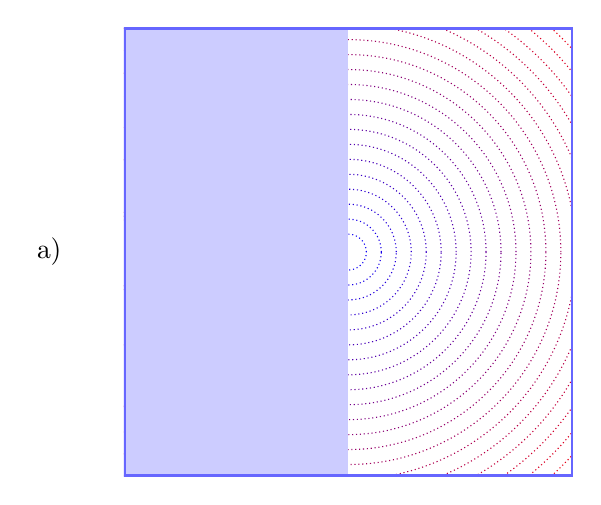
\begin{tikzpicture}[scale=1.9]
            \node[] at (-2, 0) {a)};
            \begin{scope}
                \clip (-1.5, -1.5) rectangle (1.5, 1.5);
                \foreach \cRadius in {1, ..., 22}
                    \pgfmathsetmacro\cColor{\cRadius/22*100}
                    \draw[red!\cColor!blue, densely dotted] (0, 0) circle (0.02+\cRadius*0.1); 
                    
                \fill[blue!20] (-1.5, -1.5) rectangle (0, 1.5);
                \draw[blue!60, ultra thick] (-1.5, -1.5) rectangle (1.5, 1.5);
            \end{scope}
        \end{tikzpicture}
        \qquad
        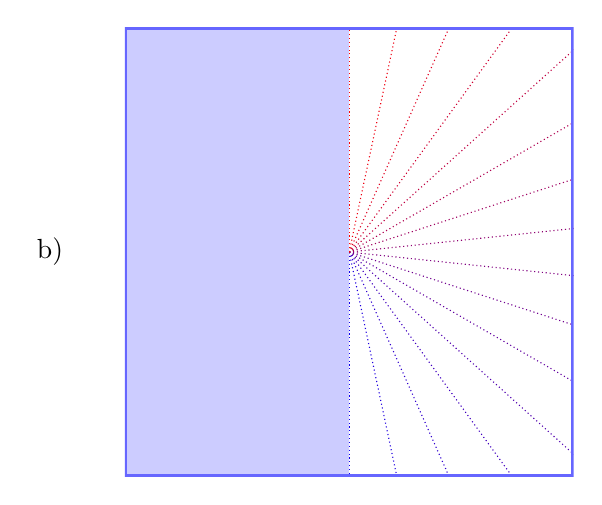
\begin{tikzpicture}[scale=1.9]
            \node[] at (-2, 0) {b)};
            \begin{scope}
                \clip (-1.5, -1.5) rectangle (1.5, 1.5);
                \foreach \cAngle in {1, ..., 16}
                    \pgfmathsetmacro\cColor{\cAngle/16*100}
                    \draw[red!\cColor!blue, densely dotted] (0, 0) -- (\cAngle* 180 / 15 -102:3); 
                \fill[blue!20] (-1.5, -1.5) rectangle (0, 1.5);
                \draw[blue!60, ultra thick] (-1.5, -1.5) rectangle (1.5, 1.5);
            \end{scope}
        \end{tikzpicture}
    \end{center}
    \caption{Schéma représentant l'extraction de caractéristiques à partir de l'espace de Fourier. En a), l'utilisation de cercles concentriques depuis l'origine, schématisé en pointillés ; En b), l'extraction selon une direction.}
    \label{fig:scheme_fourier_features}
\end{figure}\par

La transformée de Fourier se résume à la décomposition d'une donnée en une somme de fréquences. Dans le cas d'une image, cette transformation donne lieu à une représentation, dans laquelle les basses fréquences, au centre, représentent une forme d'homogénéité au sein d'une image tandis que les hautes fréquences, en extérieur, sont associées à de fortes zones de transitions. Cette transformation conserve également l'orientation des fréquences, représentée à l'aide d'un angle formé à partir de l'origine. En revanche, bien que la transformée de Fourier permette de décrire parfaitement la composition fréquentielle de l'image, elle ne peut en localiser la provenance des fréquences~\cite{Wiltgen2008}. Cet espace reste néanmoins approprié à la caractérisation d'images texturées, et a suscité un grand intérêt au milieu des années 1980~\cite{Persoon1986}. Différentes mesures ont été proposées dans cet espace afin de caractériser des textures~:
\begin{itemize}
    \item l'extraction d'information à partir \textbf{de cercles concentriques} réguliers~\cite{Smach2008a, Wiltgen2008} afin d'isoler l'information propre à chaque intervalle de fréquences (\Cref{fig:scheme_fourier_features} - a),
    \item l'extraction d'information à partir \textbf{de directions} en partance du centre vers l'extérieur de la transformée à angles constants~\cite{Wiltgen2008} (\Cref{fig:scheme_fourier_features} - b).
\end{itemize}
Ces deux travaux préconisent l'extraction d'une valeur de moyenne et d'un écart-type sur différentes régions de l'espace fréquentiel afin de qualifier les phénomènes précédemment présentés~\cite{Smach2008a, Wiltgen2008}. 

L'une des expériences menée par Wiltgen et al.~\cite{Wiltgen2008} se base sur la transformée de Fourier, et extrait \textbf{38 descripteurs} du spectre de magnitude~:
\begin{itemize}
    \item \textbf{22 descripteurs} correspondent à la moyenne calculée sur des rayons répartis de manière équidistante du centre du spectre (\Cref{fig:scheme_fourier_features} - a),
    \item \textbf{16 descripteurs} correspondent à la moyenne calculée sur des directions à intervalles constants (\Cref{fig:scheme_fourier_features} - b).
\end{itemize}
La transformée de Fourier est effectuée dans le reste de ce travail par la bibliothèque logicielle \textit{SciPy} \cite{Virtanen2020}.\par

\begin{figure}[H]
    \centering
    \includegraphics[width=0.75\textwidth]{contents/chapter_5/resources/scheme_dwt.pdf}
    \caption{Principe de la décomposition en ondelettes appliquée aux images~\cite{Livens1997}. La décomposition est réalisée en trois temps. Un filtrage passe bas (L) et passe haut (H) sont réalisés selon la direction horizontale, puis selon la direction verticale. Enfin, un sous échantillonnage de coefficient 2 est appliqué afin d'obtenir une matrice de même taille que l'image d'origine.}
    \label{fig:scheme_dwt}
\end{figure}\par 

La transformée en ondelettes possède divers avantages dont une bonne capacité de localisation, par translation de l'ondelette mère, et la possibilité de prendre en considération plusieurs échelles d'analyse, par homothétie~\cite{Livens1997,Wiltgen2008}. Concernant le choix de l'ondelette mère, celui-ci ne semble pas affecter la qualité des caractéristiques extraites~\cite{Fatemi1996, Livens1997} bien que, l'un des auteurs préconise le choix d'ondelettes symétriques ou anti-symétriques~\cite{Livens1997}. Néanmoins, les ondelettes de Daubechies et de Haar sont privilégiées lors de ces diverses expérimentations fréquentielles, les diverses références littéraires s'orientant vers  celles-ci~\cite{Wiltgen2008,Halimi2017a}. La décomposition en ondelettes sur images se réalise en trois étapes successives~: 
\begin{inlinerate}
    \item de filtrage passe-bas et passe-haut horizontal,
    \item de filtrage passe-bas et passe-haut vertical,
    \item puis une étape de sous-échantillonnage afin de réduire la quantité d'informations généré après ces deux précédentes étapes.
\end{inlinerate} Ce processus en trois temps est schématisé sur la \Cref{fig:scheme_dwt} et les opérations de transformée en ondelettes sont effectuées à l'aide de la bibliothèque logicielle \textit{PyWavelets}~\cite{lee2006}.\par

Ainsi, les expériences sur la base de descripteurs en fréquences sont réalisées en plusieurs temps. Dans un premier temps, la performance de la transformation de \textbf{Fourier} et de la transformation en ondelettes de \textbf{Daubechies} mais également de \textbf{Haar} est mesurée sur la séparation des divers groupes d'images. Dans un second temps, la méthode de \textbf{Wiltgen} et al. employant une combinaison de descripteurs de l'espace de Fourier est évaluée dans ces même conditions~\cite{Wiltgen2008}. La \Cref{tab:number_features_frequency} synthétise le nombre associé de caractéristiques extraites par ces diverses méthodes d'extraction fréquentielles.\par

\begin{table}[H]
    \centering
    \begin{tabular}{ll}
        \toprule
        \textbf{Méthode}                        & \textbf{Nombre de caractéristiques}   \\ \hline
        Fourier                                 & 10 / 20 / 30                          \\ \hline
        Ondelettes de Daubechies                & 12                                    \\ \hline
        Ondelettes de Haar                      & 12                                    \\ \hline
        Wiltgen~\cite{Wiltgen2008} - Fourier    & 38 (22+16)                             \\
        \bottomrule
    \end{tabular}
    \caption{Liste des méthodes fréquentielles évaluées dans ce chapitre et leur nombre de caractéristiques extraites associées.}
    \label{tab:number_features_frequency}
\end{table}\par
\clearpage

\subsection{Méthode d'apprentissage par transfert de connaissances}
Les méthodes d'apprentissage par transfert de connaissances sont un champ d'application relativement récent de l'apprentissage automatique. Le principe est de réutiliser des connaissances précédemment acquises, dans le but de résoudre de nouveaux problèmes plus rapidement, voire plus efficacement. Pour cela, ce champs vise à proposer des techniques permettant la transposition de connaissances d'une ou plusieurs tâches sources à une tâche cible~\cite{QiangYang2010}.\par

Le phénomène conjoint d'engouement pour les \gls{cnn} et la complexité des architectures récentes pour le traitement des images a accentué les recherches en ce sens. En effet, les techniques d'apprentissage par transfert de connaissances sont une réponse efficace à de nombreuses problématiques autour de l'entraînement des \gls{cnn}, comme~: 
\begin{itemize}
    \item les \textbf{contraintes de suffisance de données}, notamment de données convenablement structurées et annotées disponibles publiquement,
    \item le \textbf{complexité de l'entraînement}, comprenant le réglage des divers paramètres de ces réseaux (augmentations des données, fonction d'optimisation, \ldots),
    \item et les \textbf{contraintes matérielles nécessaires}, regroupant les aspects matériels dédiés au support de l'entraînement de ces architectures.
\end{itemize}\par

Certains domaines d'application ont vu apparaître de nombreuses bases de données publiques, contribuant à résoudre partiellement la contrainte liée aux données et permettant la mesure des performances de système de traitement de l'image. Parmi celles-ci, peuvent être citées~: 
\begin{inlinerate}
    \item la \textbf{base MNIST}, pour mesurer l'aptitude de systèmes dédiés à la reconnaissance de chiffres écrits à la main~\cite{lecun2010},
    \item les \textbf{bases CIFAR10 et CIFAR100}, permettant l'évaluation de systèmes de reconnaissance d'objets sur des image miniatures~\cite{Krizhevsky}, 
    \item et plus récemment, la \textbf{base ImageNet} pour la reconnaissance d'objets sur des images de taille commune~\cite{Deng2008}. 
\end{inlinerate}\par

Actuellement, la base ImageNet est l'une des plus sollicitées pour entraîner et évaluer les architectures de \gls{cnn} actuelles. Outre sa taille, cette base propose des niveaux d'annotations variées, dont 1000 classes sont proposées. De plus, une très grande diversité d'échantillons est mise à disposition pour chaque classe pour un total de plus de 14 millions d'images. Selon certaines études, ce nombre d'images reste néanmoins sur-dimensionné vis-à-vis du nombre d'éléments nécessaires à l'entraînement de ces réseaux~\cite{Huh2016}.\par

Parallèlement à ce phénomène de mise à disposition de bases de données, sont ouverts publiquement des défis visant à démontrer l'efficacité de chaînes de traitement pour gérer ces données. De nombreuses avancées ont été réalisées sur la base ImageNet, à l'aide d'architectures de \gls{cnn} régulièrement mises à disposition de la communauté. Parmi ces réseaux peuvent être cités les réseaux AlexNet~\cite{Krizhevsky2012}, GoogLeNet~\cite{Szegedy2015}, VGG~\cite{Simonyan2014}, Inception-V3~\cite{Szegedy2016}, ResNet~\cite{He2016} et Inception-ResNet~\cite{Szegedy2017}, avec respectivement comme précisions 0,54, 0,68, 0,71, 0,76, 0,78, and 0,80 sur la base ImageNet~\cite{Canziani2016}.\par

Néanmoins, la mise à disposition de la communauté de ces bases de données massives et de ces architectures ne permet pas de lever les deux verrous liés au contraintes d'entraînement et matérielles de ces réseaux. C'est donc particulièrement le partage de modèles de \gls{cnn} pré-entraînés, couplé aux principes d'apprentissage par transfert de connaissances, qui a suscité l'intérêt de nombreux travaux dont certains appliqués à l'imagerie médicale~\cite{Litjens2017}. Ainsi, la majeure partie de ces réseaux pré-entraînés est obtenu à l'aide de la base ImageNet, bien qu'aucune justification formelle n'ait été fournie à ce propos~\cite{Huh2016}.\par
 
\begin{figure}[H]
    \centering
    \includegraphics[width=\linewidth]{contents/chapter_5/resources/scheme_transfer_learning.pdf}
    \caption{Schéma représentant l'apprentissage par transfert par \gls{cnn}. Le réseau est entraîné sur des données et annotations d'une problématique \textit{source}. Puis, les paramètres de la partie liée à l'extraction de caractéristiques sont réemployés au sein d'une nouvelle problématique \textit{cible}.}
    \label{fig:scheme_transfer_learning}
\end{figure}\par

L'apprentissage par transfert sur \gls{cnn} se décompose en deux procédés majeurs~: 
\begin{inlinerate}
    \item d'une part, \textbf{l'extraction de caractéristiques} moins coûteuse en ressources matérielles et temps,
    \item et d'autre part, \textbf{le réglage fin} qui nécessite à l'inverse plus de temps et de ressources matérielles. 
\end{inlinerate}
Au sein de cette partie, le principe d'extraction de caractéristiques est développé afin de limiter les contraintes d'apprentissage, schématisée sur la \Cref{fig:scheme_transfer_learning}. Le principe consiste dans un premier temps à retirer les couches responsables de la classification du problème cible, puisque spécifiques au problème initial. Ces couches sont généralement des couches dites totalement connectées, qui vont pondérer l'importance des zones d'activation jusqu'aux classes respectives. Dans un second temps, les couches responsables de l'extraction de caractéristiques sont conservées puis figées, en partant du postulat que ces caractéristiques sont suffisamment variées et adaptées à d'autres problématiques du traitement d'image. Enfin, ces couches sont combinées à de nouvelles couches totalement connectées ou à des modèles de classification~\cite{Litjens2017}.\par 

À cette fin, une première stratégie consiste à aplatir l'information des couches d'extraction par une étape de \textit{Flatten} (littéralement \textit{Applatissement}), transformant celle-ci d'un format de matrice 3D à un vecteur 1D (voir \Cref{fig:scheme_global_pooling} - Gauche). Néanmoins, l'une des problématiques résultantes concerne la dimension spatiale souvent importante de ces caractéristiques extraites. En effet, la dimension spatiale de ces données sera réduite par les couches convolutionelles selon leurs paramètres dépendants de l'architecture choisie. Ainsi, les paramètres de décalage, de pas ou encore de taille du noyau de convolution sont autant de paramètres qui affectent la dimension spatiale de sortie. Pour pallier cette information conséquente, des couches dites de \textit{Global Pooling} ont été introduites dans la littérature, et consistent à réduire l'information spatiale d'une carte d'activation à une unique valeur dont le principe est schématisé sur la \Cref{fig:scheme_global_pooling} - Droite. Les principales fonctions mises à disposition sont la fonction maximum et moyenne, donnant respectivement lieu à des couches de \textit{Global Maximum Pooling} (ou \textit{Global Pooling - Maximum}) et de \textit{Global Average Pooling} (ou \textit{Global Pooling - Moyen}). D'autres fonctions sont également développées, mais la littérature s'accorde à préférer l'utilisation des couches de \textit{Global Pooling - Maximum}~\cite{christlein2019}.\par

\begin{figure}[H]
    \centering
    \includegraphics[width=\linewidth]{contents/chapter_5/resources/scheme_global_pooling.pdf}
    \caption{Schéma représentant l'aplatissement et la réduction d'information par \textit{Global Pooling} au sein de \gls{cnn}. Le réseau est entraîné sur des données sources, généralement plus complètes. Puis, les paramètres de la partie liée à l'extraction de caractéristiques sont conservés et réemployés au sein d'une nouvelle problématique cible.}
    \label{fig:scheme_global_pooling}
\end{figure}\par

Bien que la majeure partie des travaux en imagerie médicale s'oriente vers l'architecture Inception-V3, son efficacité n'a pas été formellement démontrée au sein des applications médicales. La raison la plus probable expliquant le choix de cette architecture est la mise à disposition de ses modèles pré-entraînés par la plupart des librairies de \gls{cnn}~\cite{Litjens2017}. Les différentes expériences sur l'apprentissage par transfert se focalisent sur des architectures relativement récentes pré-entraînées sur la base d'image ImageNet et proposées par la bibliothèque \textit{Keras Applications}~\cite{chollet2015a}. Afin de traiter les images dans leur intégralité, ces expérimentations ne considèrent que des réseaux dont les couches d'extraction de caractéristiques sont purement convolutionnelles et donc indépendantes de la taille de l'entrée. Ainsi, sont considérées les architectures de \gls{cnn} représentatives des avancés dans le domaine durant la dernière décennie, dont VGG-16, Inception-V3, ResNet-50 et Inception-ResNet. L'ensemble des réseaux employés et nombre de paramètres extraits associés sont résumés au sein de la \Cref{tab:number_features_transferlearning}. Finalement, la manipulation des \ac{cnn} est réalisée à haut niveau grâce à la bibliothèque logicielle \textit{Keras}~\cite{chollet2015} et est couplée à la bibliothèque de bas niveau \textit{Tensorflow}~\cite{Tensorflow2016}.\par

\begin{table}[H]
    \centering
    \begin{tabular}{lll}
    \toprule
    \textbf{Architecture}               & Global Pooling   & \textbf{Nombre}    \\ \hline
    \multirow{2}{*}{VGG-16}             & Maximum          & 512                \\ \cline{2-3}
                                        & Moyenne          & 512                \\ \hline
    \multirow{2}{*}{Inception-V3}       & Maximum          & 2048               \\ \cline{2-3}
                                        & Moyenne          & 2048               \\ \hline
    \multirow{2}{*}{ResNet-50}          & Maximum          & 2048               \\ \cline{2-3}
                                        & Moyenne          & 2048               \\ \hline
    \multirow{2}{*}{Inception-ResNet}   & Maximum          & 1536               \\ \cline{2-3}
                                        & Moyenne          & 1536               \\
    \bottomrule
    \end{tabular}
    \caption{Liste des architectures de \gls{cnn} employées dans ce chapitre et leur nombre de caractéristiques extraites associées.}
    \label{tab:number_features_transferlearning}
\end{table}\par
\clearpage

\subsection{Analyse préliminaire des méthodes d'extraction}
Cette analyse préliminaire de l'information a pour but de montrer l'impact des méthodes d'extraction de caractéristiques précédemment citées sur le jeu de données mis à disposition. D'une part, cette sous-section propose d'observer l'application des méthodes de transformations précédentes sur deux images typiques de tissus \textbf{malin} et \textbf{bénin}. D'autre part, la capacité de séparation des images de chacune des méthodes précédentes est observée sur l'ensemble des données.\par

Tout d'abord, la présence de motifs plus lisses et moins contrastés au sein des images bénignes peut-être constaté, à l'inverses des motifs présents dans les images malignes. Un exemple de l'application de \gls{glcm} de premier ordre sur des images typiques est visible sur la \Cref{fig:example_glcm}. Il est possible d'observer une uniformité de cette information quelle que soit la direction observée, allant dans le sens de l'utilisation de la moyenne sur les caractéristiques proposées par Haralick et al.~\cite{Wiltgen2008}. Enfin, cette transformation montre une certaine cohérence des transitions dans les images avec des valeurs présentes en majorité sur la diagonale. Néanmoins, ce phénomène semble plus intense sur l'image bénigne, traduisant des transitions plus douces que sur l'image maligne.\par

\begin{figure}[H]
    \centering
    \includegraphics[width=\linewidth]{contents/chapter_5/resources/example_glcm.pdf}
    \caption{Exemple d'extraction de \gls{glcm} de second ordre sur deux images typique. En haut, un cas d'image bénigne ; En bas, une image pathologique typique de \gls{lm}.}
    \label{fig:example_glcm}
\end{figure}\par

La \Cref{fig:example_fft} met en application la transformée de Fourier centrée sur ces deux même images. L'observation du module de cette transformation permet de constater une information plus présente en intensité sur les basses fréquences que sur les hautes fréquences de l'image bénigne, là où sur l'image maligne cette information au centre forme une tâche plus diffuse. En revanche et après une lecture rapide, la direction ne semble pas apporter d'information pertinente comme suggéré par le travail de Wiltgen et al.~\cite{Wiltgen2008}.\par

Enfin, la \Cref{fig:example_wavelet_db4} reflète cette décomposition d'ondelettes de Daubechies tandis que la \Cref{fig:example_wavelet_haar} donne un aperçu de cette même méthode par ondelettes de Haar. L'application de ces transformations permet de constater que les ondelettes de Haar semblent plus propices à isoler les zones de fortes transition que celle de Daubechies. Néanmoins, pour ces deux types d'ondelettes, les décompositions de l'image bénigne semble plus homogène que celle de l'image maligne. De même, l'extraction des hautes fréquences sur l'axe vertical et horizontal semble plus adaptée que l'extraction combinée de ces deux axes pour l'image maligne.\par

\begin{figure}[H]
    \centering
    \includegraphics[width=\linewidth]{contents/chapter_5/resources/example_fft.pdf}
    \caption{Exemple de transformée de Fourier centrée appliquée à deux images typiques, représentation selon le module et la phase. En haut, un cas d'image bénigne ; En bas, une image pathologique typique de \gls{lm}.}
    \label{fig:example_fft}
\end{figure}\par

\begin{figure}[H]
    \centering
    \includegraphics[width=\linewidth]{contents/chapter_5/resources/example_wavelet_db4.pdf}
    \caption{Exemple de transformée en ondelettes de Daubechies appliquée à deux images typiques. En haut, un cas d'image bénigne ; En bas, une image pathologique typique de \gls{lm}.}
    \label{fig:example_wavelet_db4}
\end{figure}\par

\begin{figure}[H]
    \centering
    \includegraphics[width=\linewidth]{contents/chapter_5/resources/example_wavelet_haar.pdf}
    \caption{Exemple de transformée en ondelettes de Haar appliquée à deux images typiques. En haut, un cas d'image bénigne ; En bas, une image pathologique typique de \gls{lm}.}
    \label{fig:example_wavelet_haar}
\end{figure}\par

Dans le but d'évaluer la séparation des classes, l'emploi de la réduction par l'\gls{pca} est privilégié. En effet, les données utilisés dans ce manuscrit contiennent un grand nombre de dimensions et ce malgré l'extraction de caractéristiques, rendant le problème difficile à analyser visuellement. De nombreuses techniques de réduction de l'information permettant une meilleure visualisation sont proposées dans la littérature, comme par exemple le T-SNE~\cite{Maaten2008} mais dont le principal inconvénient réside dans le nombre de degrés de liberté proposés. Néanmoins, l'\gls{pca} est une technique communément acceptée à cette fin~\cite{Himberg2001} et possède l'avantage de ne pas être dépendante de ce type de paramètres. Les informations de variance propre à ces deux axes de projection, ainsi que pour chaque classe leur centre et leur dispersion sur la base de l'écart-type sont proposés pour chaque méthode d'extraction.\par

Ainsi, la \Cref{fig:visualisation_spatial} met en évidence cette technique pour l'ensemble des méthodes spatiales d'extraction. Par ces méthodes, la variance expliquée provenant des deux axes de projection semblent à même de fournir l'intégralité de la variance de ces données. Les caractéristiques extraites à l'aide des techniques d'extraction de premier ordre ne semblent pas suffisante à séparer les diverses classes. En effet, les centres de masses et leur dispersion semblent assez similaires, notamment pour les données bénignes et malignes. De plus, la séparation des classes ne semble pas marquée dans ces divers schémas d'extraction, et les classes bénignes et saines se chevauchent lorsque les méthodes employant les caractéristiques d'Haralick et al. sont utilisées. Par ailleurs, la distribution des méthodes employant ces caractéristiques semble similaire, suscitant de faibles différences entre elles.\par

\begin{figure}[H]
    \centering
    \begin{subfigure}{.49\textwidth}
      \includegraphics[width=\textwidth]{contents/chapter_5/resources/visualisation_spatial_FirstOrder.png}
    \end{subfigure}
    \begin{subfigure}{.49\textwidth}
      \includegraphics[width=\textwidth]{contents/chapter_5/resources/visualisation_spatial_Haralick.png}
    \end{subfigure}
    
    \begin{subfigure}{.49\textwidth}
      \includegraphics[width=\textwidth]{contents/chapter_5/resources/visualisation_spatial_HaralickMean.png}
    \end{subfigure}
    \begin{subfigure}{.49\textwidth}
      \includegraphics[width=\textwidth]{contents/chapter_5/resources/visualisation_spatial_WiltgenSpatial.png}
    \end{subfigure}
    
    \caption{Visualisation des caractéristiques obtenues par techniques d'extraction spatiales et projection \gls{pca} sur les deux premières composantes.}
    \label{fig:visualisation_spatial}
\end{figure}\par

La \Cref{fig:visualisation_frequency} permet de mettre en évidence la distribution des données extraites par les méthodes d'extraction fréquentielle. Ainsi, les méthodes basées sur l'extraction de caractéristiques de Fourier semblent posséder une distribution similaire quel que soit le nombre de caractéristiques extraites. De plus, la méthode de Fourier proposée par Wiltgen~\cite{Wiltgen2008}, proposant d'extraire des caractéristiques selon diverses directions, ne semble pas influer cette distribution. Du point de vue des méthodes basées sur le principe d'ondelettes, la séparation des données semble être davantage marquée, et l'impact de l'ondelette mère ne semble pas influer sur la distribution des données et des classes. Pour l'ensemble de ces méthodes, les deux premières composantes de l'\gls{pca} semblent suffisantes à exprimer la quasi-intégralité de la variance.\par

Pour finir, la \Cref{fig:visualisation_transfer} recense les projections par \gls{pca} de l'ensemble des méthodes d'extraction basée sur des architecture de \gls{cnn} pré-entraînées, catégorisées sous le terme de transfert par apprentissage. Une différence notable est à remarquer entre les architectures utilisant une couche de \textit{Global Pooling - Moyen} et celle utilisant une couche de \textit{Global Pooling - Maximum}. En effet, la séparation entre classes est marquée de manière plus importante lorsque qu'une couche de \textit{Global Pooling - Moyen} est employée. De plus, cette séparation semble être plus prononcée sur les architectures Inception-V3 et ResNet-50, Enfin, par ces méthodes la variance exprimée sur les deux premières composantes n'est que de 20\% à 40\%. Ce dernier constat s'explique par la grande quantité d'informations initialement proposée par ces architectures, soit entre 512 et 2048 caractéristiques extraites en comparaison d'une ou quelques dizaines pour les méthodes manuelles.\par

\begin{figure}[p]
    \centering
    \begin{subfigure}{.49\textwidth}
      \includegraphics[width=\textwidth]{contents/chapter_5/resources/visualisation_frequency_Fourier10.png}
    \end{subfigure}
    \begin{subfigure}{.49\textwidth}
      \includegraphics[width=\textwidth]{contents/chapter_5/resources/visualisation_frequency_Fourier20.png}
    \end{subfigure}
    
    \begin{subfigure}{.49\textwidth}
      \includegraphics[width=\textwidth]{contents/chapter_5/resources/visualisation_frequency_Fourier30.png}
    \end{subfigure}
    \begin{subfigure}{.49\textwidth}
      \includegraphics[width=\textwidth]{contents/chapter_5/resources/visualisation_frequency_WiltgenFourier.png}
    \end{subfigure}
    
    \begin{subfigure}{.49\textwidth}
      \includegraphics[width=\textwidth]{contents/chapter_5/resources/visualisation_frequency_Haar.png}
    \end{subfigure}    
    \begin{subfigure}{.49\textwidth}
      \includegraphics[width=\textwidth]{contents/chapter_5/resources/visualisation_frequency_Daubechies.png}
    \end{subfigure}
    
    \caption{Visualisation des caractéristiques obtenues par techniques d'extraction fréquentielles et projection \gls{pca} sur les deux premières composantes.}
    \label{fig:visualisation_frequency}
\end{figure}\par

\begin{figure}[p]
    \centering
    \begin{subfigure}{.49\textwidth}
      \includegraphics[width=\textwidth]{contents/chapter_5/resources/visualisation_transfer_VGG16Avg.png}
    \end{subfigure}
    \begin{subfigure}{.49\textwidth}
      \includegraphics[width=\textwidth]{contents/chapter_5/resources/visualisation_transfer_VGG16Max.png}
    \end{subfigure}
    
    \begin{subfigure}{.49\textwidth}
      \includegraphics[width=\textwidth]{contents/chapter_5/resources/visualisation_transfer_InceptionV3Avg.png}
    \end{subfigure}
    \begin{subfigure}{.49\textwidth}
      \includegraphics[width=\textwidth]{contents/chapter_5/resources/visualisation_transfer_InceptionV3Max.png}
    \end{subfigure}
    
    \begin{subfigure}{.49\textwidth}
      \includegraphics[width=\textwidth]{contents/chapter_5/resources/visualisation_transfer_ResNetAvg.png}
    \end{subfigure}
    \begin{subfigure}{.49\textwidth}
      \includegraphics[width=\textwidth]{contents/chapter_5/resources/visualisation_transfer_ResNetMax.png}
    \end{subfigure}
    
    \begin{subfigure}{.49\textwidth}
      \includegraphics[width=\textwidth]{contents/chapter_5/resources/visualisation_transfer_InceptionResNetAvg.png}
    \end{subfigure}
    \begin{subfigure}{.45\textwidth}
      \includegraphics[width=\textwidth]{contents/chapter_5/resources/visualisation_transfer_InceptionResNetMax.png}
    \end{subfigure}
    
    \caption{Visualisation des caractéristiques obtenues par techniques d'extraction basées sur des réseaux de type \gls{cnn} pré-entraînés sur la base ImageNet et projection \gls{pca} sur les deux premières composantes.}
    \label{fig:visualisation_transfer}
\end{figure}\par

\clearpage


%%%%%%%%%%%%%%%%%%%%%%%%%%%%%%%%%% 
%%%%%%%%%%%%%%%%% PRE TRAITEMENTS
\section{Pré-traitements de caractéristiques}
Cette partie dédiée au pré-traitement de caractéristiques, se consacre à l'ensemble des transformations opérées après extraction de l'information par le biais des techniques évoquées en \Cref{chap:feature_extraction}. Au sein de cette section sont abordées les diverses solutions pouvant parfaire la classification des images \gls{mcr}. En effet, de nombreuses contraintes peuvent affecter le bon déroulement de la classification~:
\begin{itemize}
    \item un \textbf{déséquilibre des annotations} des divers types de tissus a séparé bien que celui-ci ait été minimisée,
    \item un \textbf{nombre de caractéristiques} trop important conduisant à du sur-apprentissage ou à des difficultés à séparer le problème (voir l'extraction de caractéristiques par \gls{cnn}),
    \item ou encore \textbf{une information non consistante}.
\end{itemize}\par

Ainsi, cette partie tente de répondre à ces questions à l'aide de différents domaines d'étude visant à corriger tout ou partie de ces éléments. Ces solutions sont abordées d'un point de vue logique en termes de processus de classification. Dans un premier temps, la \textbf{normalisation} des caractéristiques est présentées ainsi que son intérêt au sein de processus de classification. Dans un second temps, les méthodes de \textbf{réduction de l'information} sont proposées dans le cadre de l'extraction de caractéristiques par \gls{cnn} afin de limiter la quantité de ces dernières. Finalement, le \textbf{balancement de données} et ses principales stratégies sont mises à disposition du lecteur.

\subsection{Réduction de dimensions}
Dans le domaine de l'apprentissage automatique, la réduction de dimensions est une technique qui permet de diminuer le nombre de dimensions afin de rendre un problème moins complexe, tout en conservant une information suffisante à la résolution du problème. Également, elle est un moyen de se prévenir du «Fléau de la dimension», phénomène qui met en perspective d'une part la croissance exponentielle de l'ajout de nouvelles dimensions à la dilution des divers échantillons dans cet espace. Ce dilemme a pour principales conséquences d'augmenter la complexité d'un problème, la durée nécessaire à sa résolution mais également d'engendrer des risques de sur-apprentissage.\par

Les caractéristiques extraites par méthode spatiales et fréquentielles étant assez restreintes (respectivement de 14 à 56 variables et, de 10 à 39 variables), l'impact de la réduction de dimension n'est pas étudié sur ces méthodes. En revanche, le nombre des caractéristiques extraites par méthode de transfert de connaissance est suffisamment important (entre 512 et 2048 variables) pour justifier de l'utilisation de cette réduction et d'étudier leur impact sur ces cas particuliers.\par

À cette fin, deux catégories de méthodes cohabitent~: d'une part les méthodes de sélection de caractéristiques qui réduisent l'espace en décimant certaines dimensions jugées non pertinentes à la résolution du problème ; d'autre part les méthodes par projection ou transformation de l'espace existant qui réduisent et modifient les valeurs existantes. Dans la mesure où ces techniques s'appliquent sur les méthodes d'extraction par transfert de connaissances, cette investigation ne porte que sur cette seconde catégorie de méthodes. En effet, les méthodes par sélection de caractéristiques ne semblent pas pertinentes dans le cadre de caractéristiques auto-déterminées par des réseaux profonds.\par

L'\gls{pca} est l'une de ces techniques, dont l'idée majeure est de retirer l'information redondante pour ne conserver que l'information de variance, supposée contenir l'information. Cette méthode cherche ainsi à identifier les axes selon lesquels la variation des données est maximisée. Il sera ensuite nécessaire de déterminer un nombre d'axes suffisant à séparer le problème (réduction du nombre de caractéristiques). Ainsi, ce travail retient les seuils de la littérature les plus pertinents de cette variance cumulée, à savoir des valeurs de 95\%, 97,5\% et 99\%.\par

L'\gls{lda} est une seconde technique employée à une fin de réduction de l'information, pour laquelle sont recherchés des axes de projection qui maximisent la variance inter-groupe. Pour comparaison, la variance est le résultat de la somme de la variance intra-groupe et inter-groupe. De manière similaire à la précédente technique, sont retenus des seuils de variance cumulée de 95\%, 97,5\% et 99\%.\par

La \Cref{tab:summary_reduction_methods} reprend ces diverses méthodes ainsi que leurs paramètres mis en oeuvre conjointement à l'utilisation des méthodes d'extraction de caractéristiques sur base de transfert de connaissances.\par 

\begin{table}[H]
    \centering
    \begin{tabular}{lll}
        \toprule
        \textbf{Méthode}       & \textbf{Paramètre}                 & \textbf{Valeurs}                      \\ \midrule
        \gls{pca}              & \multirow{2}{*}{Variance expliquée}& \multirow{2}{*}{[95\%, 97,5\%, 99\%]} \\ \cline{1-1}
        \gls{lda}              &                                    &                                       \\ 
        \bottomrule
    \end{tabular}
    \caption{Liste des méthodes de réduction employées et leurs paramètres associés.}
    \label{tab:summary_reduction_methods}
\end{table}\par

\subsection{Normalisation de caractéristiques}
\label{subsec:features_normalisation}
Selon le domaine d'étude visée, la normalisation de caractéristiques peut être l'une des étapes cruciales quant au bon déroulement de ce processus de classification. Cette recherche a été amenée à considérer cet aspect suite à la dégradation de résultats au sein d'un travail proche de la thématique de ce manuscrit portant sur la classification d'images de dermatoscopie~\cite{Celebi2007}.\par

Il est communément admis que des méthodes tels que les \gls{knn} dont le principe repose sur des critères de distance, peuvent être fortement affectées par des caractéristiques non normalisées. Pour d'autres méthodes de classification, cette normalisation des caractéristiques fait davantage appel à un bon sens vis-à-vis de leur principe de fonctionnement. Certains travaux mettent en évidence la dégradation des performances sur les \gls{svm}~\cite{Juszczak2002} mais également les réseaux de neurones~\cite{Celebi2007}.\par

Diverses méthodes ont ainsi été proposées afin de remédier à ces défauts de distribution de l'information. L'un de ces travaux propose de réduire l'erreur de classification de modèles \gls{svm} par l'apport de normalisations tenant compte de la variance, du maximum ou encore conjointement du minimum et du maximum~\cite{Juszczak2002}. Le travail mené par Celebi et al.~\cite{Celebi2007} propose une normalisation des caractéristiques à l'aide de la \textit{Cote Z} ou \textit{Standard score}, c’est-à-dire par soustraction de la moyenne au sein d'un même groupe de caractéristiques puis par division de l'écart-type de ce même groupe.\par

Afin de couvrir au mieux cette problématique de normalisation, deux des méthodes majeures de la littérature sont envisagées pour la suite de cette sous-section, dont l'\Cref{eq:scaling_methods} reprend les expressions sous forme mathématique. Ainsi, sont considérées~:
\begin{itemize}
    \item la normalisation par \textit{Mininimum / Maximum}~\cite{Juszczak2002},
    \item et la normalisation \textit{Standard}~\cite{Celebi2007}.
\end{itemize}\par

\begin{equation} 
    \label{eq:scaling_methods}
    \begin{split}
    Minimum/Maximum&=\frac{X-min(X)}{max(X)-min(X)}  \\
    Standard&=\frac{X-\mu{}}{\sigma}	    
    \end{split}
\end{equation}

\subsection{Balancement de données}
\label{subsec:balancement}
L'une des problématiques associées de manière récurrente à l'apprentissage sur des données réelles est celle de la répartition homogène des annotations, en opposition aux domaines impliquant des données synthétiques pouvant provenir de modèles génératifs par exemple. Ces déséquilibres d'annotations sont qualifiés sous le terme anglophone de \textit{class imbalance}~\cite{Prati2009, He2009}.\par

Ces déséquilibres sont propres à de nombreux domaines d'applications, mais touchent essentiellement des champs d'activités dans lesquels la tâche visée correspond à la détection d'événements isolés au sein d'une population, comme par exemple~: 
\begin{inlinerate}
    \item les comportements déviants (fraude bancaire~\cite{Phua2004}),
    \item le respect de critère de qualité (vérification de pièces industrielles~\cite{Wu2018}),
    \item ou encore d'anormalités cliniques (cancers ou autres pathologies cliniques~\cite{Celebi2007}).
\end{inlinerate}\par

Certains choix peuvent permettre de limiter l'impact d'un déséquilibre d'annotations. Ainsi, la sélection d'une métrique adéquate peut permettre de limiter la dépendance au données~: la substitution de la précision par des mesures telles que l'\gls{auc}~\cite{Celebi2007} ou le \fscore{} sont des solutions pertinentes dans de telles situations. Néanmoins, la plupart des modèles de classification échouent à classifier convenablement les données dans des situations de forts déséquilibres. Ces modèles préfèrent prédire constamment la classe majoritaire, pour minimiser le coût de l'erreur~\cite{Huang2013}. Dans le cadre de modèles basés sur des arbres de décision, la stratégie générale propose de déterminer les critères majeurs de séparation par partitionnement successif des données. Ce partitionnement conduit inéluctablement à un affaiblissement des classes minoritaires~\cite{He2009}. Deux catégories d'approches coexistent pour solutionner ces déséquilibres~\cite{Huang2013}, d'une part les approches par augmentation ou décimations des diverses catégories d'annotation, et d'autres part les approches algorithmiques qui consistent à pondérer la valeur des annotations afin de prendre en considération le déséquilibre de l'information~\cite{Ting2002,He2009,Thai2010}.\par

En premier lieu, ces déséquilibres de classes peuvent être corrigés par des méthodes simples permettant de pallier ces défauts~\cite{Prati2009, He2009}. Une première catégorie de ces méthodes consiste à \textbf{sous-échantillonner} les données jusqu'à obtenir une égalité entre les classes. Son principe le plus simple est celui du \textbf{sous-échantillonnage aléatoire} consistant à décimer de manière aléatoire les données des classes majoritaires afin d'égaler les échantillons de la classe minoritaire. À l'inverse, une autre catégorie consiste à \textbf{sur-échantillonner} les données possédées afin d'obtenir à nouveau une égalité entre classes. Le principe le plus simple est celui du \textbf{sur-échantillonnage aléatoire} consistant à dupliquer aléatoirement les échantillons des classes minoritaires afin d'égaler le nombre d'éléments de la classe majoritaire. Le schéma en \Cref{fig:scheme_data_balancing} reprendre l'idée de ces deux principes.\par

En second lieu, des approches par correction des données plus avancées ont été proposées dans la littérature afin de compléter les méthode de sur-échantillonage et sous-échantillonage. L'un des exemples majeurs de ces méthodes de sur-échantillonage est la méthode \gls{smote}~\cite{Chawla2002}, dont le principe permet de générer par interpolation de nouvelles instances en choisissant aléatoirement une première instance \textit{a} et de prendre aléatoirement parmi ses plus proches voisins une seconde instance \textit{b}. En ce qui concerne les méthode de sous-échantillonage, peuvent être citées la méthode \gls{tl}~\cite{Tomek1976} et \gls{enn}~\cite{Wilson1972} utilisées pour enlever les incohérences au sein des données. Néanmoins, ces méthodes seules possèdent diverses lacunes et sont solutionnées à l'aide de nouvelles approches qualifiées d'\textit{hybrides} mêlant ces deux aspects. Parmi cette nouvelle catégorie, ce travail considère l'approche \textbf{\gls{smote} + \gls{tl}} et l'approche \textbf{\gls{smote} + \gls{enn}} dont les principes consistent à synthétiquement augmenter les données par la méthode \gls{smote}, puis à nettoyer les données constituées d'instances réelles et synthétiques par la méthode \gls{tl} ou \gls{enn}.

\begin{figure}[H]
    \centering
    \includegraphics[width=\linewidth]{contents/chapter_5/resources/scheme_data_balancing.pdf}
    \caption{Schéma des deux stratégies principales de balancement de données. À gauche, la stratégie de sous-échantillonnage, dans laquelle des éléments sont aléatoirement choisis jusqu'à réduire l'ensemble des classes au nombre d'éléments de la classe minoritaire ; À droite, la stratégie de sur-échantillonnage, dans laquelle les éléments des classes minoritaires sont dupliqués aléatoirement. }
    \label{fig:scheme_data_balancing}
\end{figure}\par

En opposition à ces méthodes dédiées, \textbf{les approches par pondération} des échantillons consistent à gérer le déséquilibre des annotations en appliquant des poids d'importance différente selon la provenance de l'échantillon lors de l'apprentissage du modèle. Cette approche par défaut est privilégiée puisqu'elle permet de contrer de manière assez intuitive ces déséquilibres.\par

Dans l'optique de récapituler cette partie, les méthodes utilisées dans le but de corriger le déséquilibre des données sont référencée dans la \Cref{tab:summary_balancement_methods}. Afin de traiter au mieux cette tâche, le balancement de données par les différentes stratégies évoquées est réalisé avec l'aide de la librairie logicielle \textit{Imbalanced-learn}~\cite{Lemaitre2017}. La correction par pondération est réalisée avec l'aide de la bibliothèque logicielle \textit{Scikit-learn}~\cite{pedregosa2011}.\par

\begin{table}[H]
    \centering
    \begin{tabular}{ll}
        \toprule
        \textbf{Catégorie}                  & \textbf{Méthode}          \\ \hline
        Sous-échantillonnage                & Aléatoire                 \\ \hline
        Sur-échantillonnage                 & Aléatoire                 \\ \hline
        \multirow{2}{*}{Hybride}            & \gls{smote} + \gls{tl}    \\ \cline{2-2}
                                            & \gls{smote} + \gls{enn}   \\ \bottomrule
    \end{tabular}
    \caption{Liste des diverses méthodes de balancement mises en œuvre pour corriger les déséquilibre de données.}
    \label{tab:summary_balancement_methods}
\end{table}\par

\section{Processus de prédiction}
Cette section dédiée au processus de prédiction se consacre à la dernière étape de traitement des données au sein du processus de classification supervisé. D'une part, son objectif est de présenter les divers modèles de classification utilisés pour la séparation de l'information. D'autre part, son objectif est de mettre en exergue le processus d'évaluation et les raisons ayant justifié ces choix.\par

\subsection{Méthodes de prédiction}
Afin d'œuvrer à la séparation des échantillons en notre possession sur la base de leurs caractéristiques, divers modèles de classification sont sollicités et pour lesquels les performances sont évaluées. En effet, bien que les avantages et inconvénients de la plupart d'entre eux aient été évoqués au sein de la \Cref{sec:models_settings}, seules les performances de classification mesurées sur le jeu de données de référence sont retenues.\par

\begin{table}[H]
    \centering
    \begin{tabular}{cll}
        \toprule
        \textbf{Modèle}                                 & \textbf{Hyperparamètre}   & \textbf{Valeurs}                          \\ \midrule
        \multirow{4}{*}{\gls{cart}}                     & Profondeur maximum        & [3, $\infty$]                             \\ \cmidrule{2-3} 
                                                        & Critère de qualité        & [Gini, Entropie]                          \\ \cmidrule{2-3}   
                                                        & Caractéristiques maximum  & [1, 2, 3, 4, 5, 6, 7, 8, 9]               \\ \cmidrule{2-3}   
                                                        & Échantillons minimum      & [1, 2, 3, 4, 5, 6, 7, 8, 9]               \\ \midrule 
        \multirow{4}{*}{\gls{rf}}                       & Profondeur maximum        & [3, $\infty$]                             \\ \cmidrule{2-3} 
                                                        & Critère de qualité        & [Gini, Entropie]                          \\ \cmidrule{2-3}   
                                                        & Caractéristiques maximum  & [1, 2, 3, 4, 5, 6, 7, 8, 9]               \\ \cmidrule{2-3}   
                                                        & Échantillons minimum      & [1, 2, 3, 4, 5, 6, 7, 8, 9]               \\ \midrule 
        \multirow{4}{*}{\gls{gb}}                       & Profondeur maximum        & [3, $\infty$]                             \\ \cmidrule{2-3}
                                                        & Critère                   & [MSE, MAE]                                \\ \cmidrule{2-3} 
                                                        & Caractéristiques maximum  & [1, 2, 3, 4, 5, 6, 7, 8, 9]               \\ \cmidrule{2-3}   
                                                        & Échantillons minimum      & [1, 2, 3, 4, 5, 6, 7, 8, 9]               \\ \midrule 
        \gls{svm} - Noyau linéaire                      & C                         & [0,001, 0,01, 0,1, 1, 10, 100, 1000]      \\ \midrule
        \multirow{2}{*}{\gls{svm} - Noyau RBF}          & C                         & [0,001, 0,01, 0,1, 1, 10, 100, 1000]      \\ \cmidrule{2-3}   
                                                        & Gamma                     & [0,001, 0,01, 0,1, 1, 10, 100, 1000]      \\ \midrule 
        \multirow{5}{*}{\gls{mlp}}                      & Couche cachées            & [(20,), (20,20,), (20,20,20,)]            \\ \cmidrule{2-3}
                                                        & Activation                & [Tanh, ReLu]                              \\ \cmidrule{2-3}
                                                        & Solveur                   & [SGD, Adam]                               \\ \cmidrule{2-3}
                                                        & Alpha                     & [0,001, 0,01, 0,1, 1, 10, 100, 1000]      \\ \cmidrule{2-3}
                                                        & Taux d'apprentissage      & [Constant, Adaptatif]                     \\ \bottomrule 
    \end{tabular} 
    \caption{Table recensant l'ensemble des modèles de classification et leurs hyperparamètres évalués lors des expériences de ce travail.}
    \label{tab:image_classification_models_hyperparameters}
\end{table}\par

Dans un premier temps, le modèle \textbf{\gls{cart}} est utilisé afin de réaliser la séparation des données, son choix étant motivé par l'un des travaux dont la thématique est similaire à celle de ce travail~\cite{Wiltgen2008}. Néanmoins, ces modèles tendent au sur-apprentissage dans des contextes où les dimensions sont nombreuses, ainsi sont utilisées de manière complémentaires les modèles \textbf{\gls{rf}}~\cite{Breiman2001} et \textbf{\gls{gb}} plus aptes à gérer cet aspect. Dans un second temps, les modèles \textbf{\gls{svm}} à noyaux \textit{linéaires} et à \textit{base radiale} sont employés pour cette même tâche de séparation des données, et sont motivés par leur utilisation dans de nombreux contextes de classification pour lesquels ils ont été démontrés comme robustes~\cite{Smach2008a}. Ces modèles sont également employés dans des contextes de classification de lésion de la peau~\cite{Celebi2007}. Enfin, la piste des \textbf{\gls{mlp}} est envisagée afin d'envisager cette problématique de manière non linéaire.\par

Afin d'obtenir les meilleurs performances sur ces modèles, les hyperparamètres associés à chacun d'entre eux sont affinés en respectant la procédure de la prochaine sous-section. Néanmoins, un compromis entre le temps d'exécution et le nombre de ces valeurs est nécessaire, conduisant ce travail à opter pour celles les plus couramment utilisées. L'ensemble des modèles de classification mais également leurs hyperparamètres et leurs valeurs associés sont recensés dans la \Cref{tab:image_classification_models_hyperparameters}. Par ailleurs, les modèles de classification employés par ce travail proviennent de la bibliothèque logicielle \textit{Scikit-learn}~\cite{pedregosa2011}.\par

\subsection{Procédure d'évaluation}
Pour réaliser l'évaluation, est employée une validation croisée imbriquée déjà discutée dans le \Cref{sec:models_settings}. Cette structure de validation est choisie car moins sujet au biais~\cite{Cawley2010}, de plus une valeur de $k$ comprise entre 5 et 10 pour l'évaluation est démontrée empiriquement comme un bon compromis entre biais et variance~\cite{James2000}. Les expériences de ce chapitre sont réalisées avec une valeur $k$ de quatre pour leur évaluation afin de réduire la durée de calcul à un temps raisonnable et de deux lots pour la validation, leur combinaison représente un bon compromis vis-à-vis des expériences de chapitre. La répartition de ces lots sur les données de \gls{mcr} exploités dans ce manuscrit est visible sur la \Cref{fig:visualisation_folds}.\par

\begin{figure}[H]
    \centering
    \includegraphics[width=0.8\linewidth]{contents/chapter_5/resources/visualisation_folds.png}
    \caption{Visualisation des divers lots d'évaluation utilisés pour l'évaluation des processus de classification.}
    \label{fig:visualisation_folds}
\end{figure}\par

Afin de régler les hyperparamètres et d'évaluer les performances des divers modèles, ce travail opte pour une métrique de type \fscore{} également discutée dans le \Cref{sec:models_settings}. En effet, cette métrique est robuste face à des déséquilibres d'annotations, tels que ceux rencontrés sur le jeu de données exploité. De plus, elle représente conjointement sous une unique mesure les valeurs de \textit{précision} et de \textit{rappel}. Son expression est binaire, elle sera ainsi calculée pour chaque classe dont la valeur est pondérée par le ratio du nombre d'échantillons disponibles dans chaque classe respective.\par

Ces expériences sont menées en plusieurs étapes successives, et débutent par l'évaluation de l'ensemble des méthodes d'extraction de caractéristiques conjointement à la normalisation de l'information selon la méthode de \textit{Minimum/Maximum} et la méthode \textit{Standard}. Aucun des tests menés n'est réalisé sur les caractéristiques brutes (sans normalisation), les expériences menées au préalable ne permettant pas de faire converger les modèles de classification dans un temps raisonnable de calcul.\par
 
\begin{figure}[H]
    \centering
    \includegraphics[width=\linewidth]{contents/chapter_5/resources/visualisation_scaling_PCA.pdf}
    \includegraphics[width=\linewidth]{contents/chapter_5/resources/visualisation_scaling_LDA.pdf}
    \caption{Visualisation de l'influence de la réduction des dimensions appliquée au deux premières composantes principales, sur un échantillon constitué arbitrairement de 500 images issue des données de \gls{mcr} mise à disposition de ces travaux. En haut, technique de réduction basée sur le \gls{pca} ; En bas, technique de réduction basée sur le \gls{lda}. À gauche, un processus procédant à la réduction puis à la normalisation ; À droite, un processus procédant à la normalisation puis à la réduction.}
    \label{fig:visualisation_scaling_reduction}
\end{figure}\par

Puis, l'impact de la réduction de dimension est mesuré sur les techniques de transfert de connaissance avant de procéder à leur classification. Contrairement aux recommandations de la librairie~\textsuperscript{\ref{footnote:exemple_pca_scaling}}, ce travail adopte un schéma de type réduction de l'information suivi d'une normalisation de caractéristiques avant l'étape de classification. En effet, les caractéristiques issues de réseaux convolutionnels possèdent une distribution de valeurs consistantes, et n'affectent pas de manière significative les techniques de réduction de dimensions. En revanche, la réduction d'information par techniques de projection peut affecter la consistance de cette distribution des valeurs. Ce phénomène a notamment été observé sur un lot de 500 données choisies arbitrairement, et présentées sur la \Cref{fig:visualisation_scaling_reduction}.\par

Pour finir, ces expériences mesurent l'impact du déséquilibre des données sur les résultats de classification et évaluent la pertinence des méthodes qui visent à corriger ce déséquilibre dans ce contexte. Pour cela, les méthodes les plus pertinentes sont soumises à une classification sans correction du déséquilibre d'annotations mais également avec les divers mécanismes mentionnés dans la \Cref{subsec:balancement}, et leurs résultats sont comparés.\par

La sélection des modèles les plus pertinent se base sur les résultats à trois classes dans la mesure où ces scores sont représentatifs de la capacité à caractériser la problématique dans son ensemble. Néanmoins dans la dernière partie de cette analyse, seuls les résultats de la détection des images malignes sont détaillés dans la mesure où ceux-ci correspondent à l'objectif visé par ce travail.\par

\addtocounter{footnote}{1}
\footnotetext[\thefootnote]{Source~: Scikit-learn - \href{https://scikit-learn.org/stable/auto_examples/preprocessing/plot_scaling_importance.html}{«Importance of Feature Scaling»}. \label{footnote:exemple_pca_scaling}}
\clearpage

\section{Résultats}
Ce premier volet est mené sur les méthodes d'extraction de caractéristiques associées aux techniques de normalisation. Dans un premier temps, en terme de méthode d'extraction spatiale, un \fscore{} de 0,64 associé à un écart-type de 0,07 est obtenu par la méthode proposé par \textbf{Haralick} et al. et \textbf{sans moyenne des axes}. Ce score correspond à l'utilisation conjointe d'une normalisation de type \textbf{Minimum / Maximum} et d'un modèle \textbf{\gls{svm} avec un noyau à base radiale}. Dans un second temps, en terme de méthode d'extraction fréquentielle, un \fscore{} de 0,67 associé à un écart-type de 0,06 est obtenu par l'utilisation de l'extraction en \textbf{ondelettes de Daubechies}. Ce score correspond à l'utilisation conjointe d'une normalisation de type \textbf{Minimum / Maximum} et d'un modèle \textbf{\gls{svm} avec un noyau linéaire ou avec un noyau à base radiale}. De plus, ce score correspond également à l'utilisation conjointe d'une normalisation de type \textbf{Standard} et d'un modèle \textbf{\gls{svm} avec un noyau linéaire}. Enfin, en terme de méthode par transfert de connaissances, un \fscore{} de 0,77 associé à un écart-type de 0,04 est obtenu sur l'architecture \textbf{ResNet-50} combinée à une couche de \textbf{Global Pooling - Moyen}. Ce score correspond à l'utilisation conjointe d'une normalisation de type \textbf{Minimum / Maximum} et d'un modèle \textbf{\gls{svm} avec un noyau linéaire}. L'ensemble des résultats liés à ces expérimentations est visible sur la \Cref{fig:results_image_classification}.\par

\begin{figure}[H]
    \centering
    
    \begin{subfigure}{\textwidth}
      \includegraphics[width=\textwidth]{contents/chapter_5/resources/results_image_classification_mms.pdf}
    \end{subfigure}
    
    \begin{subfigure}{\textwidth}
      \includegraphics[width=\textwidth]{contents/chapter_5/resources/results_image_classification_ss.pdf}
    \end{subfigure}
    
    \caption{Résultats issus de la classification par les diverses techniques d'extraction et par les modèles de classification mentionnés en couleur. En haut, les résultats provenant de la normalisation de type \textit{Minimum / Maximum} ; En bas, les résultats provenant de la normalisation de type \textit{Standard}. À gauche, la représentation basée sur les valeurs moyennes ; À droite, la représentation tenant compte de l'écart-type.}
    \label{fig:results_image_classification}
\end{figure}\par

Ce second volet mesure l'impact de la réduction d'informations sur les méthodes d'extraction par transfert de connaissances. En effet, la grande quantité d'informations issues de ces techniques peut provoquer une dégradation des performances de classification, ce que tente de vérifier ce nouveau paragraphe. Seules les architectures couplées à une couche de \textit{Global Pooling - Moyen} sont évaluées, leurs performances ayant été significativement supérieures aux architectures couplées avec un \textit{Global Pooling - Maximum}. D'une part, un \fscore{} de 0,76 associé à un écart-type de 0,03 est obtenu sur l'architecture \textbf{ResNet-50} combinée à une couche de \textbf{Global Pooling - Moyen}. Ce score provient de l'utilisation conjointe de \textbf{l'\gls{pca} avec une variance cumulée de 99\%}, d'une normalisation de type \textbf{Minimum / Maximum} et d'un modèle \textbf{\gls{svm} avec un noyau linéaire}. D'autre part, un \fscore{} de 0,73 associé à un écart-type de 0,05 est obtenu sur l'architecture \textbf{VGG-16} combinée à une couche de \textbf{Global Pooling - Moyen}. Ce score provient de l'utilisation conjointe de \textbf{l'\gls{lda} avec une variance cumulée de 95\%}, d'une normalisation de type \textbf{Standard} et d'un modèle \textbf{\gls{svm} avec un noyau linéaire}. Les résultats de ce volet de l'expérience sur les méthodes de réduction de l'information sont reportés sur la \Cref{fig:results_image_classification_reduction}.\par

\begin{figure}[H]
    \centering
    
    \begin{subfigure}{\textwidth}
      \includegraphics[width=\textwidth]{contents/chapter_5/resources/results_image_classification_reduction_mms.pdf}
    \end{subfigure}
    
    \begin{subfigure}{\textwidth}
      \includegraphics[width=\textwidth]{contents/chapter_5/resources/results_image_classification_reduction_ss.pdf}
    \end{subfigure}
    
    \caption{Résultats issus de la classification par l'utilisation de techniques de réduction combinés aux techniques d'extraction par transfert et, par les modèles de classification mentionnés en couleur. Les tracés de couleurs représentent les divers modèles évalués au cours de l'expérience. En haut, les résultats provenant de la normalisation par Minimum/Maximum ; En bas, les résultats provenant de la normalisation par score Standard. À gauche, la représentation basée sur les valeurs moyennes ; À droite, la représentation tenant compte de l'écart-type.}
    \label{fig:results_image_classification_reduction}
\end{figure}\par

Le dernière volet de ces expérimentations se destine à étudier l'impact du déséquilibre des données sur la qualité des résultats de classification. Son influence est mesuré sur les méthodes les plus performantes relatives aux précédents paragraphes de cette section, couplé aux méthodes de corrections de ces déséquilibres. Ainsi, un \fscore{} de 0,77 associé à un écart-type de 0,04 est obtenu par la méthode de transfert de connaissances basée sur l'architecture \textbf{ResNet-50} couplé à une couche de \textbf{Global Pooling - Moyen}. Ce score résulte de l'utilisation conjointe d'une normalisation \textbf{Minimum/Maximum} suivi d'un modèle \textbf{\gls{svm} à noyau linéaire} dont l'utilisation est combinée à l'utilisation \textbf{d'une pondération} dans le but de compenser le déséquilibre de données. Les résultats lié à l'étude du déséquilibre des données à trois classes sont visibles sur la \Cref{tab:results_balancement_multi}.\par

\begin{table}[H]
    \begin{tabular}{lllllll}
        \toprule
                    & Aucune        & Pond.                 & Sur-éch.      & Sous-éch.     & SMOTE+ENN     & SMOTE+Tomek   \\ \hline
        Spatial     & 0,55$\pm$0,15 & 0,61$\pm$0,09         & 0,54$\pm$0,15 & 0,58$\pm$0,11 & 0,60$\pm$0,09 & 0,56$\pm$0,16 \\
        Fréquentiel & 0,59$\pm$0,13 & 0,67$\pm$0,06         & 0,55$\pm$0,21 & 0,58$\pm$0,17 & 0,61$\pm$0,12 & 0,64$\pm$0,10 \\ \rowcolor[HTML]{E7E6E6}
        Transfert   & 0,71$\pm$0,08 & \textbf{0,77$\pm$0,04}& 0,74$\pm$0,07 & 0,72$\pm$0,05 & 0,74$\pm$0,05 & 0,74$\pm$0,05 \\
        Réduction   & 0,71$\pm$0,09 & 0,76$\pm$0,03         & 0,74$\pm$0,06 & 0,73$\pm$0,04 & 0,73$\pm$0,04 & 0,73$\pm$0,06 \\ \bottomrule
    \end{tabular}
    \caption{Résultats à trois classes issus de l'expérience mêlant les méthodes les plus performantes associée aux méthodes de balancement de données évoquées.}
    \label{tab:results_balancement_multi}
\end{table}\par

Ces même résultats sont également observés du point de vue des performances de la classe maligne. Par ce nouveau point de vue, un \fscore{} de 0,82 associé à un écart-type de 0,02 est obtenu par la méthode de transfert de connaissances basée sur l'architecture \textbf{ResNet-50} couplé à une couche de \textbf{Global Pooling - Moyen}. Comme précédemment, ce score résulte de l'utilisation conjointe d'une normalisation \textbf{Minimum/Maximum} suivi d'un modèle \textbf{\gls{svm} à noyau linéaire} dont l'utilisation est combinée à l'utilisation \textbf{d'une pondération} dans le but de compenser le déséquilibre de données. Les résultats lié à l'étude du déséquilibre des données, et adoptant le point de vue de la classe maligne, sont disponibles sur la \Cref{tab:results_balancement_malignant}.\par

\begin{table}[H]
    \begin{tabular}{lllllll}
        \toprule
                    & Aucune        & Pond.                 & Sur-éch.      & Sous-éch.     & SMOTE+ENN     & SMOTE+Tomek   \\ \hline
        Spatial     & 0,65$\pm$0,11 & 0,63$\pm$0,07         & 0,64$\pm$0,10 & 0,64$\pm$0,08 & 0,63$\pm$0,09 & 0,59$\pm$0,27 \\
        Fréquentiel & 0,70$\pm$0,09 & 0,68$\pm$0,03         & 0,66$\pm$0,09 & 0,66$\pm$0,09 & 0,61$\pm$0,22 & 0,66$\pm$0,09 \\ \rowcolor[HTML]{E7E6E6} 
        Transfert   & 0,81$\pm$0,04 & \textbf{0,82$\pm$0,02}& 0,81$\pm$0,03 & 0,79$\pm$0,01 & 0,80$\pm$0,02 & 0,82$\pm$0,03 \\
        Réduction   & 0,81$\pm$0,03 & 0,81$\pm$0,01         & 0,81$\pm$0,03 & 0,79$\pm$0,03 & 0,80$\pm$0,01 & 0,81$\pm$0,03 \\ \bottomrule 
    \end{tabular}
    \caption{Résultats de la détection de tissus malins issus de l'expérience mêlant les méthodes les plus performantes associées aux méthodes de balancement de données évoquées.}
    \label{tab:results_balancement_malignant}
\end{table}\par

Enfin, les courbes \gls{roc} permettent d'appréhender les performances de prédiction de ce système. Ainsi, les performances propres à l'ensemble de la base d'images annotées sont homogènes par cette technique avec des scores \gls{auc} dont les valeurs sont comprises entre 0,87 et 0,90, Néanmoins, une analyse \gls{roc} des lésions de types \gls{lm} et \gls{lmm} comme seules représentantes des classes malignes mettent en avant des performances moins homogènes entre les diverses classes. Ces scores \gls{auc} dont les valeurs varient entre 0,79 et 0,92 représentent une limite de ces méthodes a différencier les tissus bénins et les tissus malins. Ces diverses courbes sont visibles sur la \Cref{fig:results_image_classification_roc}.\par

\begin{figure}[H]
    \centering
    \includegraphics[width=\textwidth]{contents/chapter_5/resources/results_image_classification_roc.pdf}
    \caption{Résultats sous forme de courbes \gls{roc}. À gauche, résultats sur l'ensemble des lésions d'étude ; À droite, résultats excluant les lésions malignes différentes des types \gls{lm}/\gls{lmm}.}
    \label{fig:results_image_classification_roc}
\end{figure}\par

\section{Discussion}
Suite aux précédents résultats, plusieurs constats peuvent être formulés pour donner suite à la mise en pratique des méthodes d'extraction de caractéristiques. Le premier constat concerne les méthodes d'extraction spatiales, et plus particulièrement l'utilité de la méthode proposée par Haralick et al. sur les données de \gls{mcr} utilisées dans ce travail. En revanche, l'ajout de mesures de premier ordre ne semble pas ou peu impacter les performances. Le second constat concerne les méthodes d'extraction fréquentielles, et en particulier la supériorité sur ces données de l'extraction de caractéristiques par la transformée en ondelettes comparé à l'extraction de caractéristiques par la transformée de Fourier. Ce travail à également confirmé la faible influence de l'ondelette mère sur ces même données, bien que l'ondelette mère de Daubechies soit plus performante dans ce travail. Enfin, le dernier constat concerne la proposition de méthodes sur la base de transfert de connaissance à partir d'architectures de \gls{cnn} pré-entraînées, dont les résultats sont significativement supérieurs aux autres méthodes. Sur l'ensemble des architectures évaluées, la combinaison mêlant l'architecture ResNet-50 pré-entraîné sur ImageNet à une couche de \textit{Global Pooling - Moyen} produit les résultats les plus pertinent et sont plus amplement développée dans la suite de ce travail.\par

En termes de modèles de classification, l'un de ces constats concerne le modèle \gls{svm} avec noyau linéaire dont les performances et la stabilité sont les plus pertinentes dans la plupart des expériences menées lors de ce chapitre. Par opposition, le modèle \gls{svm} avec noyau à base radiale a été essentiellement pertinent à l'aide d'une normalisation par Minimum / Maximum, sa performance et stabilité chutant de manière drastique lorsque les caractéristiques sont nombreuses. Du côté des méthodes basées sur les arbres de décision, ces techniques sont globalement peu influencées par les méthodes de normalisation. Comme attendu, les \gls{cart} sont performants dans la plupart des situations, exceptées celles par transfert de connaissances dans lesquelles le nombre de caractéristiques est trop important. À cette fin, les techniques de \gls{rf} et \gls{gb} ont été particulièrement adaptées, les \gls{gb} étant légèrement moins stables que les \gls{rf}. Pour finir cette analyse des modèles, l'utilisation de \gls{mlp} dans le but d'observer l'effet de la non-linéarité semble ne pas avoir aidé à améliorer la classification.\par

Afin de compenser le nombre élevé de caractéristiques extraites par les \gls{cnn}, des techniques de réduction mises en place afin de pallier ce problème sont évaluées. Dans ce travail, leur utilisation réduit les performances de prédiction mais également la stabilité en augmentant sensiblement l'écart-type. Bien que moins performants, des résultats intéressants sont obtenues dans une configuration utilisant ResNet-50 et l'\gls{pca} avec une variance expliquée de 99\% permettant de retirer près des trois quarts des caractéristiques. La relation entre variance expliquée et caractéristiques par cette méthode est visible sur la \Cref{fig:results_image_classification_pca_variance}.\par

\begin{figure}[H]
    \centering
    \includegraphics[width=0.8\textwidth]{contents/chapter_5/resources/results_image_classification_pca_variance.pdf}
    \caption{Analyse de la variance expliquée cumulée par l'application de l'\gls{pca}. Le nombre de caractéristiques est représenté pour des variances expliquées de 95\% en vert, 99\% en jaune et 99,5\% en orange.}
    \label{fig:results_image_classification_pca_variance}
\end{figure}\par

La dernière méthode mise en œuvre pour optimiser les performances de classification des images concerne le balancement des annotations. Dans le contexte de ce manuscrit, la méthode par pondération est préférée aux autres méthodes de sa catégorie car elle propose une correction du non-balancement à moindre frais, tout en garantissant de meilleure performances sur l'ensemble des expériences menées.\par

En conclusion, ce premier chapitre expérimental a permis de mettre au point un processus permettant de traiter les données \gls{mcr}. Les expérimentations menées permettent d'accomplir une classification avec un \fscore{} de 0,77 associé à un écart-type de 0,04 pour 3 classes et de 0,82 associé à un écart-type de 0,02 pour la classification d'éléments malins. De plus ce processus a permis l'obtention d'une \gls{auc} de 0,90 sur l'ensemble des données et de 0,85 sur les données excluant les lésions différentes des types \gls{lm} et \gls{lmm}. Néanmoins, des améliorations sur la qualité de ce processus de diagnostic sont à prévoir, ainsi que sur la possible prise en compte de l'intersection d'évènements tels que la présence de tissus caractéristiques auprès de follicules pileux.\par
\renewcommand{\thechapter}{\arabic{chapter}}
\setcounter{chapter}{5}

\chapter{Amélioration du diagnostic image}
\label{chap:chapter_6}
\chapterintro
Les expérimentations conduites lors du précédent chapitre ont tenté d'apporter une première réponse pour la séparation des images \acrlong{mcr} et menée selon les annotations saines, bénignes ou encore malignes. Pour cela, ce travail s'est intéressé aux méthodes permettant de caractériser au mieux les aspects de texture de ces images par l'extraction de caractéristiques pertinentes mais également aux méthodes de classification permettant la meilleure séparation des images selon les précédentes annotations.\par

Néanmoins, ces méthodes abordent la problématique par une compréhension globale des images de \acrlong{mcr}, dont le principe même est considéré comme une limitation dans ce nouveau chapitre. Dans ce chapitre, de nouveaux schémas sont considérés afin d'améliorer le diagnostic de ces images. Ainsi, des méthodes exploitant le principe de résolution multiple, de fenêtre glissante, ou encore exploitant les \acrlong{cnn} par réglage fin de bout en bout sont utilisés dans ce nouveau chapitre.\par

\newpage

\section{Méthodologie}
Lors du précédent chapitre, diverses approches ont été proposées afin de comprendre les composants essentiels d'une image dans son intégralité, et de permettre ainsi la séparation des éléments \textbf{sains}, \textbf{bénins} et \textbf{malins}. Cette approche suppose que l'information extraite afin de caractériser ces images est suffisante pour permettre une séparation selon les trois précédentes annotations. Cette hypothèse n'est que partiellement juste puisqu'une même image de la modalité de \gls{mcr} peux comporter divers types de tissus selon ces trois annotations, dont la hiérarchie d'inclusion entre annotations est visible sur la \Cref{fig:scheme_image_improvement_annotations_hierarchy}.\par

\begin{figure}[H]
    \centering
    \includegraphics[width=0.7\textwidth]{contents/chapter_6/resources/scheme_image_improvement_annotations_hierarchy.pdf}
    \caption{Schéma représentatif de la relation hiérarchique entre les annotations. Les images malignes peuvent ainsi contenir des tissus bénins et sains ; Les images bénignes peuvent contenir des tissus sains ; Les images saines ne contiennent que des tissus sains.}
    \label{fig:scheme_image_improvement_annotations_hierarchy}
\end{figure}\par

Dans ce nouveau chapitre dédié à l'amélioration du diagnostic de l'image, les observations du \cref{chap:chapter_5} sont reprises, en privilégiant notamment l'utilisation de la \textbf{normalisation par Minimum / Maximum} et le \textbf{modèle \gls{svm} à noyau linéaire}. Les représentants les plus performants des méthodes d'extraction de caractéristiques sont également conservés dans ce travail, dont~:
\begin{itemize}
    \item pour la \textbf{catégorie de méthodes spatiales}, les caractéristiques définies par Haralick et al.,
    \item pour la \textbf{catégorie de méthodes fréquentielles}, les caractéristiques sur base d'extraction en ondelettes,
    \item pour la \textbf{catégorie de méthodes de transfert de connaissances}, l'architecture ResNet-50 associée à une couche de Global Pooling - Moyenne.
\end{itemize}\par

Ainsi, des schémas alternatifs sont envisagés afin d'extraire une information suffisante nécessaires à la séparation des données de la modalité de \gls{mcr}. Ce chapitre débute par la présentation de \textbf{méthodes par échelles multiples}, en supposant que l'information comporte plusieurs niveaux d'interprétations. Puis, s'ensuit la description de \textbf{méthodes par fenêtre glissante} pour extraire localement une information propre aux tissus. Afin d'étendre ce principe d'approche locale, ce travail s'intéresse à l'utilisation du \textbf{réglage fin sur des \gls{cnn}}. Enfin, ce chapitre propose \textbf{une analyse des résultats} issus de ces diverses méthodes, lesquels aboutissent à \textbf{une discussion} permettant d'approfondir ces résultats.\par
\clearpage

\section{Approche par échelles multiples}
Comme évoqué précédemment, les traitements réalisés jusqu'alors ne permettent qu'une compréhension globale de l'image. Cette vision de l'extraction de caractéristiques peut être erronée si l'on suppose une interprétation de l'image à divers niveaux de compréhension.\par

C'est ainsi que des hypothèses de compréhensions de l'image à échelles multiples ont émergé, bien que peu relatées dans la littérature. Ces approches ont été employées à différentes fins~:~
\begin{inlinerate}
    \item de détection de frontières dans un contexte d'images naturelles~\cite{Ren2008},
    \item de segmentation d'images~\cite{Santos2012,Arbelaez2014},
    \item de détection d'objets~\cite{Felzenszwalb2008} ou d'actions~\cite{Pedersoli2011},
    \item ou encore de classification d'images médicales~\cite{Alsaih2016,Tang2017}.
\end{inlinerate} En termes d'images~\gls{mcr} appliquée au domaine de la dermatologie, le travail de Wiltgen et al.~\cite{Wiltgen2008} semble le plus proche et propose entre autre le traitement de ces données par échelles multiples. Ainsi, cette section est scindée en deux parties respectives, avec d'une part l'application de ce principe à la décomposition en ondelettes et d'autre part l'application de ce principe à des techniques d'extractions spatiales.\par 

\subsection{Décomposition en ondelettes par échelles multiples}
La première approche par échelles multiples se base sur la décomposition en ondelettes. En effet, ce principe a été démontré comme judicieux dans de nombreux domaines impliquant l'analyse d'images~\cite{Carvalho2004}. Cette décomposition peut être effectuée sous la forme de schémas qualifiés soit de \textbf{diadique}, soit de \textbf{pyramidal}. Ces deux modes sont schématisés sur la \Cref{fig:scheme_image_improvement_dwt_decomposition}. L'un des articles de référence de ce travail préconise l'utilisation du schéma de décomposition diadique pour l'extraction de caractéristiques de texture sur images \gls{mcr}~\cite{Wiltgen2008}. Pour cela, cet article se focalise sur l'utilisation d'une \textbf{ondelette mère de Daubechies} et emploie cette transformée à cinq niveaux de détail successifs sous forme d'arbre diadique. Les mesures associées à chaque bande de fréquences de la transformée sont les mêmes que dans le \Cref{chap:chapter_5} et se basent sur l'extraction de l'\textbf{écart-type}, de l'\textbf{énergie} et de l'\textbf{entropie} pour un total de \textbf{39 caractéristiques}. Suite aux résultats obtenus et présentés dans le \Cref{chap:chapter_5}, ce procédé est également évalué selon \textbf{l'ondelette mère de Haar}.\par

\begin{figure}[H]
    \centering
    \includegraphics[width=\textwidth]{contents/chapter_6/resources/scheme_image_improvement_dwt_decomposition.pdf}
    \caption{Schématisation deux principaux types de décomposition successives par ondelettes. En a), schéma de décomposition multi-échelle en ondelettes dit \textbf{diadique} ; En b), schéma de décomposition multi-échelle en ondelettes dit \textbf{pyramidal}.}
    \label{fig:scheme_image_improvement_dwt_decomposition}
\end{figure}\par

La seconde méthode sur lequel ce travail prend appui est une extension de la transformée en ondelettes de l'article de Wiltgen et al.~\cite{Halimi2017a}. Ainsi, cette nouvelle méthode reprend la précédente décomposition selon un schéma diadique, et en modifie le \textbf{nombre de décompositions à quatre niveaux}, au lieu des cinq initialement prévus. Selon cette même méthode, une loi normale généralisée centrée, dont la densité de probabilité $f$ est décrite par l'\Cref{eq:image_improvement_ggd}, est ajustée à la distribution de valeurs de chaque niveau de décomposition. Enfin, les auteurs de l'étude ne retiennent comme caractéristiques que \textbf{les paramètres d'échelle $\alpha$ et de forme $\beta$} de cette loi normale généralisée pour un total de \textbf{24 caractéristiques}.\par

\begin{equation}
    f(x)= \frac{\beta}{2\alpha\Gamma(1/\beta)} e^{-\left(|\frac{x}{\alpha}|\right)^\beta}
    \label{eq:image_improvement_ggd}
\end{equation}

Afin de gérer ces diverses caractéristiques, ce travail s'emploie à l'utilisation d'un \textbf{modèle de type \gls{svm} à noyau linéaire}, démontré empiriquement efficace pour la classification de données fréquentielles lors du \Cref{chap:chapter_5}. Les hyperparamètres employés afin de tirer le meilleur parti de ce modèle sont listés sur la \Cref{tab:parameters_image_improvement_multiscale_frequency}. L'implémentation du modèle \gls{svm} utilisé provient de la bibliothèque logicielle \textit{Scikit-learn}~\cite{pedregosa2011}.\par

\begin{table}[H]
    \centering
    \begin{tabular}{lll}
        \toprule
        \textbf{Modèle}                                 & \textbf{Hyperparamètres}  & \textbf{Valeurs}                          \\ \midrule
        \gls{svm} - Noyau linéaire                      & C                         & [0,001, 0,01, 0,1, 1, 10, 100, 1000]      \\ 
        \bottomrule 
    \end{tabular} 
    \caption{Table reprenant le modèle et les hyperparamètres du modèle de classification employé pour la prédiction sur les caractéristiques fréquentielles par échelles multiples.}
    \label{tab:parameters_image_improvement_multiscale_frequency}
\end{table}\par

Les étapes de transformée en ondelettes et la décomposition à différentes échelles de cette expérimentation sont réalisées à l'aide de la bibliothèque logicielle \textit{PyWavelets}~\cite{lee2006}. Quant aux opérations d'ajustement de la loi généralisée, celles-ci s'appuient sur la bibliothèque logicielle \textit{SciPy}~\cite{Virtanen2020}. L'ensemble de ces expérimentations basées sur la décomposition en ondelettes à échelles multiples sont recensées sur la \Cref{tab:wavelet_image_improvement_multiscale_nb_features} ainsi que leurs nombres de caractéristiques associées à chacune d'entre elles.\par

\begin{table}[h]
    \centering
    \begin{tabular}{ll}
        \toprule
        \textbf{Méthode}                                    & \textbf{Nombre de caractéristiques}   \\ \hline
        Ondelettes - Haar                                   & 39 (13$\times$3)   \\ \hline
        Ondelettes - Daubechies / Wiltgen~\cite{Wiltgen2008}& 39 (13$\times$3)   \\ \hline
        Halimi~\cite{Halimi2017a}                           & 24 (12$\times$2)   \\
        \bottomrule
    \end{tabular}
    \caption{Listes des méthodes sur base de décomposition par échelles multiples en ondelettes et leur nombre de caractéristiques extraites associées.}
    \label{tab:wavelet_image_improvement_multiscale_nb_features}
\end{table}\par
\clearpage

\subsection{Décomposition spatiale par échelles multiples}
Lors de la précédente sous-section, les approches par échelles multiples sur base d'extraction en ondelettes ont été présentées. Toujours dans cette optique d'approche d'échelles multiples, divers travaux se sont orientés afin de permettre une classification d'images médicales sur la base d'extraction de caractéristiques spatiales~\cite{Alsaih2016,Tzalavra2016}. Les prochaines étapes s'inspirent de ces travaux mais également des conclusions apportées par le \Cref{chap:chapter_5} sur l'extraction de caractéristiques spatiales et par transfert de connaissances. Ainsi, sont mis en œuvre deux processus par échelles multiples dans ce chapitre, présentés lors des prochains paragraphes.\par

La première méthode proposée se base sur une approche de type fusion de caractéristiques avant l'étape de classification, déjà rencontrée dans des travaux à but similaire~\cite{Pedersoli2011,Alsaih2016}. Afin de permettre l'agrégation de ces caractéristiques, une \textbf{normalisation par Minimum / Maximum} associé à un \textbf{modèle \gls{svm} à noyau linéaire} est employé, démontré efficace de manière empirique lors du \Cref{chap:chapter_5} et robuste dans des contextes à fortes dimensions. À nouveau, l'implémentation du modèle \gls{svm} employé dans ce travail provient de la bibliothèque logicielle \textit{Scikit-learn}~\cite{pedregosa2011} et les hyperparamètres utilisés par ce modèle sont recensés dans la \Cref{tab:parameters_image_improvement_models_multiscale_spatial}. Le principe de fonctionnement de cette première méthode est schématisé sur la \Cref{fig:scheme_image_improvement_multiscale_features}.\par

\begin{figure}[H]
    \centering
    \includegraphics[width=0.9\linewidth]{contents/chapter_6/resources/scheme_image_improvement_multiscale_features.pdf}
    \caption{Schéma de représentation du système par échelles multiples, sur la base d'une extraction à diverses échelles puis par l'agrégation des caractéristiques avant la procédure de classification.}
    \label{fig:scheme_image_improvement_multiscale_features}
\end{figure}\par

La seconde méthode correspond à un schéma en deux temps, dans lequel chaque modèle de prédiction est spécialisé à une échelle spatiale précise. À cette fin, est employé pour chacune de ces échelles une \textbf{normalisation par Minimum / Maximum} associée à un \textbf{modèle de type \gls{svm} à noyau linéaire} pour les raisons évoquées précédemment, dont les hyperparamètres sont recensés dans la \Cref{tab:parameters_image_improvement_models_multiscale_spatial}. Ce faisant, il est alors nécessaire de réunir ou \textbf{fusionner} ces informations en une unique décision, dont le rôle est effectué à l'aide d'\textbf{un vote à la majorité}~\cite{Kam1994,Lam1997}, dont le principe ne nécessite aucune phase d'entraînement. Cette technique est ainsi employé~:~
\begin{inlinerate}
    \item sur les \textbf{scores} définis par l'ensemble $\mathbf{R}$,
    \item mais également sur les \textbf{décisions} définies par l'ensemble $\mathbf{N}$.
\end{inlinerate} Une première méthode est mise en place à l'aide d'\textbf{une fonction de moyenne appliquée aux scores}, de laquelle est extrait le score le plus élevé. Ce schéma permet de notifier d'\textbf{une tendance globale} d'une classe par rapport aux autres. Une seconde méthode est mise en place à l'aide d'\textbf{une fonction de maximum appliquée aux scores}, de laquelle est extrait le score le plus élevé. Ce schéma permet d'isoler la classe recueillant la confiance de prédiction la plus élevée. Enfin, la dernière méthode est mise en place par recensement de la classe qui a recueilli \textbf{le plus grand nombre de décisions}. Le processus global de cette expérience est présenté sur la \Cref{fig:scheme_image_improvement_multiscale_decision}.\par

\begin{table}[H]
    \centering
    \begin{tabular}{lll}
        \toprule
        \textbf{Modèle}                                 & \textbf{Hyperparamètres}  & \textbf{Valeurs}                          \\ \midrule
        \gls{svm} - Noyau linéaire                      & C                         & [0,001, 0,01, 0,1, 1, 10, 100, 1000]      \\ 
        \bottomrule 
    \end{tabular} 
    \caption{Table recensant les paramètres du modèle de classification employé pour réaliser la prédiction par échelles multiples sur caractéristiques spatiales ou par transfert de connaissances. Ce modèle associé à ces hyperparamètres est employé pour la classification par échelle mais également pour l'agrégation des multiples échelles.}
    \label{tab:parameters_image_improvement_models_multiscale_spatial}
\end{table}\par

\begin{figure}[H]
    \centering
    \includegraphics[width=0.85\linewidth]{contents/chapter_6/resources/scheme_image_improvement_multiscale_decision.pdf}
    \caption{Schéma de représentation du système par échelles multiples, sur la base d'extractions et de prédictions à diverses échelles et par agrégation de ces décisions.}
    \label{fig:scheme_image_improvement_multiscale_decision}
\end{figure}\par

Ainsi, les diverses expériences de cette sous-section sont menées à l'aide des modes d'extraction précédemment étudiés dans le \Cref{chap:chapter_5}. Dans un premier temps, les descripteurs d'Haralick et al.~\cite{Haralick1973} sont employées et permettent l'extraction de 56 caractéristiques. Dans un second temps, le transfert de connaissances par l'utilisation de l'architecture de \gls{cnn} ResNet-50~\cite{He2016} pré-entraîné sur la base ImageNet~\cite{Canziani2016} est employé et permet l'extraction de 2048 caractéristiques. Les expériences menées lors de cette sous-section sont recensées dans la \Cref{tab:parameters_spatial_transfer_multiscale_nb_features}.\par

\begin{table}[H]
    \centering
    \begin{tabular}{llll}
        \toprule
                                                    &          & \multicolumn{2}{l}{Nombre de caractéristiques} \\ \hline
        \multirow{2}{*}{Fusion de caractéristiques} & Haralick & \multicolumn{2}{l}{224 (56$\times$4)}          \\ \cline{2-4}
                                                    & ResNet-50& \multicolumn{2}{l}{8192 (2048$\times$4)}       \\ \hline
        \multirow{2}{*}{Fusion de prédictions}      & Haralick & 56 / échelle   & \multirow{2}{*}{\begin{tabular}[c]{@{}l@{}}4 (1$\times$4) / Décisions\\ 12 (3$\times$4) / Scores\end{tabular}} \\ \cline{2-3}
                                                    & ResNet-50& 2048 / échelle &                               \\
        \bottomrule
    \end{tabular}
    \caption{Listes des méthodes sur base de décomposition par échelles multiples et leur nombre de caractéristiques extraites associées.}
    \label{tab:parameters_spatial_transfer_multiscale_nb_features}
\end{table}\par
\clearpage

\section{Approche par fenêtre glissante}
Lors de la section précédente, des schémas par échelles multiples permettant une compréhension à divers niveaux ont été évoqués. Cette nouvelle section va s'orienter vers une compréhension des données à basse échelle, en partant de l'hypothèse qu'il existe un niveau de détail pour lequel les tissus peuvent être caractérisés avec suffisamment de précision.\par

Ce type d'approche est qualifié d'approche \textbf{par fenêtre glissante} ou par \textit{sliding window}. Néanmoins, le premier terme permet de visualiser le principe de fonctionnement consistant à balayer un espace de plus grande dimension par une fenêtre de dimension inférieure. Cette technique a permis des avancées pour diverses applications, dont~:~
\begin{itemize}
    \item de la détection et localisation d'objets sur des images naturelles~\cite{Harzallah2009} ou encore de détection de cancer et de parties anatomiques sur images de radiologie~\cite{Helwan2017}, par motivation d'obtenir l'emplacement précis de certaines informations,
    \item de la détection d'anomalies sur des images histologiques mais encore de la classification de données conséquentes~\cite{Hou2016,Alqudah2019,Wei2019}, motivée par la contrainte matérielle impliquée par la taille de ces images ou par manque d'annotations.
\end{itemize}\par

Les données images de \gls{mcr} mises à la disposition de ce travail corroborent ce type de schéma, chacune d'entre elles contenant une composition de tissus divers. Ces labels au niveau de l'image répondent à une hiérarchie mise en place pour qualifier les relations entre ces tissus. Pour rappel, une annotation \textbf{maligne} qualifie une donnée comportant au minimum des tissus typiques d'une pathologie maligne mais peut également comporter des tissus bénins et sains ; une annotation \textbf{bénigne} ne comporte que des tissus bénins ou potentiellement sains. Ces relations sont représentées sur la \Cref{fig:scheme_image_improvement_annotations_hierarchy}.\par

Ce travail se distingue de certains travaux~\cite{Hou2016,Alqudah2019} dans la mesure où il bénéficie d'une base de \textit{sous-images} d'une résolution spatiale \textbf{de 250$\times$250 pixels}, annotées pour le besoin par l'un des spécialistes en dermatologie. Cette taille est un compromis entre le niveau de détail des types de tissus observables et les conclusions de Wiltgen et al., suggérant une telle résolution~\cite{Wiltgen2008}. Néanmoins, afin d'affranchir partiellement ce travail de l'influence de la taille de la fenêtre glissante, \textbf{une augmentation de ces sous-images à une résolution \textbf{de 500$\times$500 pixels} par mosaïquage} est également employée.\par

\begin{table}[H]
    \centering
    \begin{tabular}{lll}
        \toprule
        \textbf{Modèle}                                 & \textbf{Hyperparamètres}  & \textbf{Valeurs}                          \\ \midrule
        \gls{svm} - Noyau linéaire                      & C                         & [0,001, 0,01, 0,1, 1, 10, 100, 1000]      \\ 
        \bottomrule 
    \end{tabular} 
    \caption{Table reprenant le modèle et les hyperparamètres du modèle de classification employé pour la détection à basse échelle des tissus dans le processus de fenêtre glissante.}
    \label{tab:parameters_image_improvement_sliding_window_models}
\end{table}\par

Dans le but de mettre en oeuvre le schéma de détection à basse échelle, les techniques d'extraction de caractéristiques jugées les plus pertinentes du \Cref{chap:chapter_5} sont utilisées, à savoir~:~
\begin{inlinerate}
    \item la méthode d'Haralick et al. comme représentante des méthodes spatiales,
    \item la méthode en ondelette de Daubechies comme représentante des méthodes fréquentielles,
    \item et enfin la méthode d'extraction par l'architecture ResNet-50 associé à une couche de Global Pooling - Moyenne comme représentante des méthodes par transfert de connaissances.
\end{inlinerate} Cette détection à basse échelle est réalisée à l'aide d'\textbf{une normalisation par Minimum / Maximum} associé à \textbf{un modèle \gls{svm} à noyau linéaire}, cette combinaison ayant été jugée la plus pertinente lors du \Cref{chap:chapter_5} et dont les paramètres sont listés dans la \Cref{tab:parameters_image_improvement_sliding_window_models}.\par

Afin de gérer les prédictions obtenues au niveau de la fenêtre glissante, plusieurs stratégies sont envisagées sur les décisions et les scores. Ainsi, plusieurs approches sont considérées, dont~:
\begin{itemize}
    \item   une approche au niveau des \textbf{décisions}, défini par l'ensemble $\mathbf{N}$. Cette approche aboutit à un vecteur de taille 1$\times$n où n correspond au nombre d'éléments extraits dans l'image. Deux méthodes ont été définies, dont~:~
            \begin{itemize}
                \item par \textbf{priorité}, dans laquelle est privilégiée la détection d'un élément d'une classe hiérarchiquement supérieure comme décision globale à l'image,
                \item par seuils \textbf{dynamiques}, dans laquelle sont déterminés des seuils optimaux d'éléments nécessaires à chaque classe pour décréter l'appartenance à l'une d'entre elles, combiné à un système hiérarchique privilégiant les classes prioritaires.
            \end{itemize}
    \item   une approche au niveau des \textbf{scores}, défini par l'ensemble $\mathbf{R}$. Cette approche aboutit à un vecteur de taille s$\times$n où s correspond au nombre de scores de classes extrait et n correspond au nombre d'éléments extraits dans l'image. Deux méthodes ont été définies, dont~:~
            \begin{itemize}
                \item par seuil \textbf{dynamique}, dans un premier temps cette méthode procède à une réduction de l'information à l'aide d'une fonction maximum, permettant de réduire celui-ci à vecteur de taille 1$\times$s focalisé sur la confiance maximum en chaque classe. Dans un second temps, des seuils optimaux représentant la confiance minimale nécessaire sont déterminés sur ces scores, combinés là encore à un système hiérarchique privilégiant les classes prioritaires.
                \item par \textbf{classification}, le vecteur de scores est alors considéré comme un vecteur de caractéristiques fourni en entrée d'un modèle \gls{svm} linéaire, dont les hyperparamètres utilisés sont ceux de la \Cref{tab:parameters_image_improvement_sliding_window_models}.
            \end{itemize}
\end{itemize}\par

Dans ce travail, le scénario portant sur l'extraction de caractéristiques seules à l'aide de la fenêtre glissante, puis à la fusion de ces caractéristiques au niveau de l'image, n'est pas considéré. En effet, ce type de scénario génère bien trop de caractéristiques pour pouvoir être correctement traité au niveau de l'image. De plus, ce type de schéma perd l'une des motivations de cette méthode, à savoir isoler les parties d'images susceptibles de contenir les tissus d'intérêts.\par
 
Les paramètres propres à cette méthode sont visibles dans la \Cref{tab:parameters_image_improvement_sliding_window_parameters}. Afin de visualiser cette méthode, la \Cref{fig:scheme_image_improvement_sliding_features} met à disposition un schéma dans lequel ce processus est représenté.\par

\begin{table}[H]
    \centering
    \begin{tabular*}{0,6\linewidth}{l@{\extracolsep{\fill}}l}
        \toprule
        \textbf{Résolution spatiale}& \textbf{Chevauchement}\\ \hline
        250$\times$250              & 0~\%                  \\ \hline
        250$\times$250              & 25~\%                 \\ \hline
        250$\times$250              & 50~\%                 \\ \hline 
        500$\times$500              & 0~\%                  \\ \hline
        500$\times$500              & 25~\%                 \\ \hline
        500$\times$500              & 50~\%                 \\
        \bottomrule
    \end{tabular*}
    \caption{Ensemble des paramètres d'expérimentations menées par l'approche de type fenêtre glissante. L'étude de l'impact de la résolution spatiale est limitée aux valeurs de 250$\times$250 et 500$\times$500, mais également du chevauchement sur des valeurs de 0~\%, 25~\% et 50~\%.}
    \label{tab:parameters_image_improvement_sliding_window_parameters}
\end{table}\par

\begin{landscape}
\begin{figure}[H]
    \centering
    \includegraphics[width=0.8\linewidth]{contents/chapter_6/resources/scheme_image_improvement_sliding_features.pdf}
    \caption{Schéma de représentation du système de prédiction par fenêtre glissante. Ce schéma en deux temps propose de prédire sur une multitude de sous parties de l'image originale puis de fusionner les diverses prédictions afin de fournir une prédiction globale à la donnée originale. Ainsi, une première phase d'entraînement est réalisée à l'aide des sous-images. Puis, le modèle entraîné permet de prédire au niveau des images par principe de fenêtre glissante pour lequel un second modèle permet de définir quels seuils sont critiques.}
    \label{fig:scheme_image_improvement_sliding_features}
\end{figure}\par
\end{landscape}

\section{Réglage fin de réseaux de convolution}
Dans cette partie, le réglage fin des \gls{cnn} est utilisé à cette fin de problématique de classification d'images de la modalité de \gls{mcr}. En effet, ce principe est sollicité dans de nombreuses thématiques de recherche au moment de la rédaction de ce manuscrit, comme par exemple pour de la détection de plans d'intérêts sur des images par ultrasons~\cite{Chen2015}, mais aussi de plans cardiaques sur des images d'\gls{irm}~\cite{Margeta2017}. Également, ce principe est utilisé de manière très encourageante dans des applications visant à de la détection de pathologies sur des acquisitions de rayons X réalisées sur des seins~\cite{Lotter2017} ou encore sur des poumons~\cite{Gao2018}.\par

C'est de manière naturelle que cette section s'oriente en ce sens, en se consacrant à ses divers aspects à l'aide de sous-sections propre à chaque concept. Tout d'abord, une présentation du principe de réglage fin et des choix opérés est réalisé. Puis, les diverses techniques mises en œuvre pour tirer parti de ce principe sont présentés, dont~:
\begin{inlinerate}
    \item l'augmentation de données,
    \item et le programme d'apprentissage.
\end{inlinerate}\par

\subsection{Présentation et mise en oeuvre de la méthode}
Le réglage fin est une extension de l'apprentissage par transfert, dans lequel sont substituées les couches de classification initiales du réseau par de nouvelles couches adaptées au problème. Cette approche se distingue dans la mesure où tout ou partie du réseau est ré-entraîné à partir des poids existants~\cite{Tajbakhsh2016}. Ce mode d'apprentissage est utilisé lorsque les données propres au nouveau problème sont suffisantes, et permet à l'instar du simple apprentissage par transfert d'obtenir un réseau plus adapté au problème cible. Néanmoins, ce mode d'apprentissage \textbf{nécessite des ressources et un temps d'entraînement plus conséquent}.\par

Afin de procéder à ce réglage fin, il est nécessaire de déterminer une architecture cible permettant de gérer au mieux la complexité des données. Par exemple, un travail récent lors de la rédaction du manuscrit~\cite{Park2019} privilégie dans cette démarche l'utilisation d'une architecture \textit{ResNet-50}~\cite{He2016} pour la détection de lésions pulmonaires sur des images de rayons X et propose la localisation de ces dernières. Néanmoins, aucune justification ne semble avoir été apportée sur le choix de cette architecture, et aucune information n'est stipulée sur le type de \textit{Global Pooling} employé par ce travail.\par

Lors du \Cref{chap:chapter_5}, les résultats des principales architectures de \gls{cnn} pré-entraînés sur la base ImageNet ont été comparés par application du principe de transfert de connaissances. Cette expérience a permis de déterminer de manière empirique la pertinence l'\textbf{architecture de \gls{cnn} ResNet-50~\cite{He2016} associée à une couche de Global Pooling - Moyenne} sur cette problématique. Ainsi, ce travail suppose que l'architecture \textit{ResNet-50}~\cite{He2016} associée à une couche de \textit{Global Pooling - Moyenne} couplée au principe du réglage fin est en mesure de spécialiser le réseau à la problématique de lésion de la peau sur images \gls{mcr}, et d'améliorer \textit{in fine} ses performances.\par

Suivant ce constat, l'initialisation de cette architecture \textit{ResNet-50} est réalisée \textbf{à l'aide de poids issus d'un entraînement sur la base ImageNet}. Dans un premier temps, \textbf{la dernière couche totalement connectée de ce réseau sur base d'une activation \textit{softmax} est retirée}, prévue pour supporter les 1000 classes de la base de données \textit{ImageNet}. Dans un second temps, \textbf{une nouvelle couche totalement connectée de trois classes sur base d'une activation \textit{softmax} est ajoutée} afin de supporter les annotations saines, bénignes et malignes. Dans la mesure où ce travail tente de résoudre une problématique à plusieurs classes, \textbf{une fonction de coût de type entropie-croisée} est utilisée, suggérée par des travaux dont la problématique est équivalente~\cite{Barbu2018,Park2019}.\par

En termes de paramètres, la taille des lots ou \textit{batch size} \textbf{est réglée à une valeur de 8} pour des raisons de limitations matérielles. Néanmoins, une taille plus conséquente permet une meilleur stabilité de la convergence de ce dernier. De plus, il est utile de préciser que l'ensemble des données \gls{mcr} dédié à l'entraînement sont utilisées lors de chacune de ces \textit{epochs}. Le nombre d'itérations ou \textit{epochs} n'est pas stipulé, \textbf{un critère d'arrêt en cas de convergence insuffisante après 5 itérations}, dont l'estimation est réalisée sur les données d'entraînement, est jugée suffisant dans ce contexte. Enfin, ce travail emploie une optimisation de type \textit{adam} tel que suggéré par de précédents travaux~\cite{Barbu2018,Park2019}, et dont \textbf{le taux d'apprentissage est réglé à une valeur de 0,001} faute de détails sur l'implémentation.\par

Pour finir sur ces aspects de mise en oeuvre, l'ensemble de ces éléments ont été réalisés à haut niveau à l'aide de la bibliothèque logicielle \textit{Keras}~\cite{chollet2015} en association à la bibliothèque de bas niveau \textit{Tensorflow}~\cite{Tensorflow2016}.\par

\subsection{Augmentation de données}
L'augmentation de données est une technique qui permet de corriger de manière artificielle le nombre d'exemples d'une base de données par application de transformations aux données d'origine~\cite{Wong2016,Taylor2018}. Cette technique est à ne pas confondre avec les méthodes de création d'échantillons virtuels à partir de l'espace des caractéristiques pour corriger les problèmes de balancements. L'augmentation de données, au sens de cette section, permet de corriger un non-balancement des annotations, mais est essentiellement employée dans le but d'enrichir le nombre d'exemples disponibles en contraignant le \gls{cnn} à se focaliser sur des éléments jugés essentiels à la résolution de la tâche visée.\par

Dans cette sous-section, cette technique est vue selon ces deux aspects mais surtout comme le moyen d'enrichir la base d'images \gls{mcr} et ainsi d'éviter le sur-apprentissage potentiellement responsable de la dégradation des performances de prédiction. Les techniques considérées à cet effet correspondent à des transformations géométriques linéaires~\cite{Taylor2018}, opérées de manière aléatoire à chaque \textit{epochs} lors de l'entraînement. Bien évidemment, ces transformations ne sont appliquées que lors de l'entraînement, les images originales étant employées lors de l'évaluation. Les transformations considérées sont celles susceptibles de se produire dans un contexte clinique lors de l'acquisition des images, dont~:
\begin{inlinerate}
    \item la \textbf{rotation},
    \item la \textbf{translation},
    \item ou encore la \textbf{symétrie}.
\end{inlinerate} De plus, un repliement de l'information est réalisé pour combler le vide généré par ces opérations, jugé plus \textit{réaliste} sur les images traitées, que l'application d'une unique valeur de remplissage.\par

Ainsi, l'ensemble des paramètres de transformation utilisés lors de l'étape d'augmentation des données sont décrit sur la \Cref{tab:parameters_image_improvement_data_augmentation}. Cette étape s'appuie à cette fin sur le module d'augmentation de données de la bibliothèque logicielle \textit{Keras}~\cite{chollet2015}.\par

\begin{table}[H]
    \centering
    \begin{tabular}{ll}
        \toprule
        \textbf{Nom}                            & \textbf{Valeurs}      \\ \midrule
        Rotation (en degrés)                    & [0 à 45]              \\ 
        Translation Horizontale (en pourcentage)& [0 à 20]              \\ 
        Translation Verticale (en pourcentage)  & [0 à 20]              \\  
        Symétrie Horizontale                    & [Désactivée, Activée]  \\  
        Symétrie Verticale                      & [Désactivée, Activée]  \\ 
        \bottomrule 
    \end{tabular} 
    \caption{Table recensant les paramètres de transformation utilisés sur les données images de \gls{mcr} de manière aléatoire lors de l'entraînement.}
    \label{tab:parameters_image_improvement_data_augmentation}
\end{table}\par

\subsection{Programme d'apprentissage}
Le programme d'apprentissage ou \textit{Curriculum Learning} est une démarche visant par analogie à l'humain, à entraîner tout \gls{cnn} en proposant diverses tâches intermédiaires avec une difficulté croissante, afin d'accomplir avec une plus grande efficacité une tâche plus complexe. La raison technique derrière ce principe est de simplifier l'espace de recherche de la tâche cible, afin de trouver plus efficacement un minimum optimal au sein de la fonction de coût, comme suggéré par ses auteurs~\cite{Bengio2009}.\par

De récents travaux menés sur des images médicales, issue de rayons X, ont permis par cette approche d'augmenter les performance de détection de \gls{cnn} sur des cancers du sein~\cite{Lotter2017} ou encore des pathologies pulmonaires~\cite{Park2019}. La démarche suivie par ces deux travaux, est de procéder à l'extraction de sous images de taille restreinte autour des dites lésions avérées, en conservant la même propriété d'échelle que les images initiales. Cette extraction permet de réduire la résolution et la complexité du problème en proposant au réseau des images moins volumineuses et davantage focalisées sur des éléments clés afin d'éviter potentiellement des convergences non pertinentes. La gestion de données à échelles multiples sur \gls{cnn} ne donnant pas toujours lieu à des résultats suffisant~\cite{Noord2017}, une seconde étape d'entraînement est ensuite réalisée sur les images de taille réelle afin de former le réseau au problème définitif.\par

En complément de cette technique, la première phase de l'entraînement du \gls{cnn} est réalisée en deux temps. En effet, l'ajout de nouvelles couches connectées sous-entend une initialisation aléatoire de ces dernières. Ce phénomène peut conduire à une mauvaise remise en question de certains poids issus du caractère aléatoire de l'étape d'initialisation. Ainsi, une immobilisation des couches liées à l'extraction des caractéristiques est réalisée dans un premier temps (pré-entraînement), avant de procéder à l'entraînement du réseau dans sa totalité dans un second temps (entraînement). Ce processus d'entraînement en deux temps est schématisé sur la \Cref{fig:scheme_image_fine_tune}.\par

\begin{figure}[H]
    \centering
    \includegraphics[width=\linewidth]{contents/chapter_6/resources/scheme_image_improvement_image_fine_tune.pdf}
    \caption{Schéma de représentation du processus de réglage fin utilisé dans ce travail. Celui-ci se décompose d'une étape d'initialisation dans le but de substituer les couches de classification, puis un pré-entraînement permet d'initialiser les poids avant de procéder à l'entraînement.}
    \label{fig:scheme_image_fine_tune}
\end{figure}\par
\clearpage

\section{Présentation des résultats}
Lors des précédentes sections ont été décrites les méthodes envisagées dans le but d'accroître la performance des prédictions au niveau des images \gls{mcr} mais également leur compréhension. Par cette nouvelle section, les résultats obtenus par ces méthodes sont présentés. Dans une première sous-section, le protocole d'expérimentation suivi pour mesurer les performances de ces méthodes et l'organisation des résultats sont détaillés, puis dans une seconde sous-section, les résultats des diverses méthodes sont présentés.\par

\subsection{Protocole d'expérimentation}
Le protocole d'expérimentation suivi est similaire à celui du \cref{chap:chapter_5}, afin que les résultats obtenus dans ce chapitre puissent être mis en parallèle et comparés avec ceux précédemment obtenus. Pour rappel, une \textbf{validation croisée imbriquée} est employée car les métriques extraites par ce processus sont plus objectives sur les performances du système évalué que des systèmes de validation croisée standards~\cite{Cawley2010}. De plus, cette structure de validation est plus robuste face au biais~\cite{Cawley2010} et démontrée empiriquement moins sensible au biais et à la variance lorsque des valeurs de $k$ sont comprises entre 5 et 10~\cite{James2000}. Pour des critères similaires à ceux du précédent chapitre, lié au grand nombre d'expérimentations, et de comparaison avec les précédents résultats, \textbf{une valeur $k$ de 4} est choisie.\par

En terme de métrique de validation et d'évaluation, les expérimentations de ce chapitre se basent sur le \textbf{\fscore{}} permettant de représenter les mesures de précision et de rappel au sein d'une même métrique binaire. Par ailleurs, cette métrique a été employée lors du \cref{chap:chapter_5} et possède une bonne robustesse face à des déséquilibres de données. Concernant la présentation des résultats de l'évaluation, chaque méthode met à disposition du lecteur deux scores. D'une part, \textbf{un score pondéré} dont l'objectif est de fournir une indication de performance sur les trois classes que ce chapitre tente de séparer. D'autres part, \textbf{un score malin} dont l'objectif est de renseigner sur la capacité d'une méthode à isoler particulièrement les données malignes.\par

D'un point de vue organisationnel, la prochaine sous-section propose un premier volet dédié aux résultats de classification des méthodes proposées, et met en évidence les combinaisons permettant la maximisation des scores ainsi que les résultats complets à l'aide de tables prévue à cet effet. Lors du premier paragraphe, les résultats des expérimentations menées \textbf{par principe d'échelles multiples} sont présentés. Puis dans un second et troisième paragraphe, les résultats obtenus \textbf{par principe de fenêtre glissante} sont présentés à \textbf{une résolution spatiale de 250$\times$250 pixels puis de 500$\times$500 pixels}. Pour finir, un quatrième paragraphe présente les résultats des expérimentations \textbf{de \gls{cnn} associé au principe de réglage fin}.\par

Pour finir, ce chapitre propose un second volet consacré à des techniques permettant d'aller au-delà du seul score de classification. Le premier de ces paragraphes propose une solution simple permettant d'observer localement les résultats obtenus par fenêtre glissante. Ainsi, la mise en place d'un code couleur sur les décisions et les scores de prédiction superposé à l'image d'origine permet de visualiser les éléments déterminants lors de la prédiction. Puis, les paragraphes suivants apportent des pistes sur la visualisation de décisions issues de \gls{cnn} par utilisation du principe de \gls{cam}.\par
\clearpage

\subsection{Résultats des expérimentations}
Cette section suit paragraphe par paragraphe l'organisation énoncée et débute par les résultats issus de la famille de méthodes \textbf{par résolutions multiples}. Par la catégorie \textbf{par ondelettes} et à l'aide de la \textbf{méthode de Wiltgen et al.}~\cite{Wiltgen2008}, un \fscore{} de 0,65 associé à un écart-type de 0,08 est obtenu à trois classes ; un \fscore{} de 0,71 associé à un écart-type de 0,06 est obtenu sur la classe maligne. Par la catégorie de méthodes \textbf{spatiale} et à l'aide de la \textbf{méthode de fusion de caractéristiques}, un \fscore{} de 0,63 associé à un écart-type de 0,06 est obtenu à trois classes ; un \fscore{} de 0,67 associé à un écart-type de 0,07 est obtenu sur la classe maligne. Enfin, par la catégorie de méthodes par \textbf{transfert de connaissances} et à l'aide de la \textbf{méthode de fusion de caractéristiques}, un \fscore{} de 0,76 associé à un écart-type de 0,06 est obtenu à trois classes ; un \fscore{} de 0,83 associé à un écart-type de 0,02 est obtenu sur la classe maligne. Les résultats de l'expérimentation menée sur la résolution multiple sont visibles dans la \Cref{tab:results_image_improvement_multiresolution}.\par

\begin{table}[H]
    \centering
    \begin{tabular}{llcc}
        \toprule
        Catégories                  & Méthodes                      & \Fscore{} - Pondéré   & \Fscore{} - Malin     \\ \midrule
        \multirow{3}{*}{Ondelettes} & Haar                          & 0,65$\pm$0,08         & 0,70$\pm$0,06         \\
                                    & Wiltgen~\cite{Wiltgen2008}    & \textbf{0,66$\pm$0,06}& \textbf{0,71$\pm$0,06}\\
                                    & Halimi~\cite{Halimi2017a}     & 0,38$\pm$0,02         & 0,41$\pm$0,04         \\ \midrule
        \multirow{5}{*}{Spatial}    & Fusion de caractéristiques    & \textbf{0,63$\pm$0,06}& \textbf{0,67$\pm$0,07}\\
                                    & Décisions - Maximum           & 0,60$\pm$0,10         & 0,64$\pm$0,08         \\
                                    & Scores - Moyenne + Maximum    & 0,60$\pm$0,10         & 0,66$\pm$0,07         \\
                                    & Scores - Maximum + Maximum    & 0,59$\pm$0,10         & 0,65$\pm$0,08         \\
                                    & Scores - \gls{svm} Linéaire   & 0,57$\pm$0,10         & 0,65$\pm$0,04         \\ \midrule \rowcolor[HTML]{E7E6E6}
        \multirow{5}{*}{Transfert}  & Fusion de caractéristiques    & \textbf{0,76$\pm$0,06}& \textbf{0,83$\pm$0,02}\\ 
                                    & Décisions - Maximum           & 0,69$\pm$0,10         & 0,78$\pm$0,05         \\
                                    & Scores - Moyenne + Maximum    & 0,69$\pm$0,11         & 0,79$\pm$0,06         \\
                                    & Scores - Maximum + Maximum    & 0,69$\pm$0,11         & 0,79$\pm$0,06         \\
                                    & Scores - \gls{svm} Linéaire   & 0,72$\pm$0,04         & 0,79$\pm$0,03         \\
        \bottomrule
    \end{tabular}
    \caption{Résultats issus du processus de classification basé sur la classification par échelles multiples exprimées à l'aide du \fscore.}
    \vspace{-1em}
    \label{tab:results_image_improvement_multiresolution}
\end{table}

Ce second paragraphe présente les résultats obtenus à l'aide de l'approche \textbf{par fenêtre glissante}, à partir \textbf{d'une résolution spatiale de 250$\times$250 pixels}. Les résultats sont maximisés par l'utilisation de \textbf{l'extraction par transfert de connaissance} sur la base de sous-images, pour laquelle un \fscore{} de 0,91 associé à un écart-type de 0,02 est obtenu à trois classes ; un \fscore{} de 0,82 associé à un écart-type de 0,03 est obtenu sur la classe maligne. Par la catégorie de \textbf{méthodes spatiales} combinée à la méthode de \textbf{Décision - Dynamique} et \textbf{sans chevauchement}, un \fscore{} de 0,62 associé à un écart-type de 0,02 est obtenu à trois classes ; un \fscore{} de 0,68 associé à un écart-type de 0,05 est obtenu sur la classe maligne. Par la catégorie de \textbf{méthodes fréquentielles} combinée à la méthode de \textbf{Score - Classification} et \textbf{avec un chevauchement de 50~\%}, un \fscore{} de 0,61 associé à un écart-type de 0,07 est obtenu à trois classes ; un \fscore{} de 0,68 associé à un écart-type de 0,06 est obtenu sur la classe maligne. Pour finir, par la catégorie de \textbf{méthodes de transfert de connaissances} combinée à la méthode de \textbf{Score - Classification} et \textbf{avec un chevauchement de 50~\%}, un \fscore{} de 0,78 associé à un écart-type de 0,03 est obtenu à trois classes ; un \fscore{} de 0,82 associé à un écart-type de 0,02 est obtenu sur la classe maligne. Les résultats détaillés obtenus par principe de fenêtre glissante dont la résolution spatiale est de 250$\times$250 pixels, sont présentés dans la \Cref{tab:results_image_improvement_sliding_window}.\par

\afterpage{\begin{landscape}
\begin{table}[p]
    \centering
    \begin{tabular}{lllcccccc}
		\toprule
		\multirow{2}{*}{Taille}     & \multirow{2}{*}{Chevauchement}& \multirow{2}{*}{Mode}     & \multicolumn{2}{c}{Spatial}                   & \multicolumn{2}{c}{Fréquence}                 & \multicolumn{2}{c}{Transfert}                 \\
		                            &                               &                           & Pondéré               & Malin                 & Pondéré               & Malin                 & Pondéré               & Malin                 \\ \midrule
		250                         & Aucune                        & Sous-images               & 0,67$\pm$0,10         & 0,41$\pm$0,13         & 0,72$\pm$0,07         & 0,44$\pm$0,10         & \textbf{0,91$\pm$0,02}& \textbf{0,82$\pm$0,03}\\ \midrule
		\multirow{12}{*}{250}       & \multirow{4}{*}{0~\%}          & Décision - Priorité       & 0,52$\pm$0,02         & 0,67$\pm$0,04         & 0,44$\pm$0,06         & 0,65$\pm$0,05         & 0,58$\pm$0,04         & 0,71$\pm$0,05         \\ 
							        &                               & Décision - Dynamique      & \textbf{0,62$\pm$0,02}& \textbf{0,68$\pm$0,05}& 0,57$\pm$0,06         & 0,67$\pm$0,04         & 0,75$\pm$0,02         & 0,80$\pm$0,03         \\
							        &                               & Score - Dynamique         & 0,54$\pm$0,02         & 0,63$\pm$0,04         & 0,50$\pm$0,08         & 0,66$\pm$0,05         & 0,70$\pm$0,03         & 0,76$\pm$0,02         \\
							        &                               & Score - Classification    & 0,60$\pm$0,05         & 0,66$\pm$0,04         & 0,59$\pm$0,08         & 0,65$\pm$0,07         & 0,78$\pm$0,03         & 0,81$\pm$0,03         \\ \cline{2-9}
							        & \multirow{4}{*}{25~\%}         & Décision - Priorité       & 0,49$\pm$0,10         & 0,67$\pm$0,10         & 0,41$\pm$0,10         & 0,65$\pm$0,10         & 0,53$\pm$0,05         & 0,70$\pm$0,09         \\
							        &                               & Décision - Dynamique      & 0,62$\pm$0,07         & 0,68$\pm$0,11         & 0,58$\pm$0,08         & 0,66$\pm$0,09         & 0,75$\pm$0,03         & 0,80$\pm$0,04         \\
							        &                               & Score - Dynamique         & 0,52$\pm$0,03         & 0,59$\pm$0,06         & 0,49$\pm$0,08         & 0,66$\pm$0,10         & 0,72$\pm$0,04         & 0,78$\pm$0,03         \\
							        &                               & Score - Classification    & 0,62$\pm$0,06         & 0,71$\pm$0,06         & 0,57$\pm$0,10         & 0,66$\pm$0,08         & 0,78$\pm$0,03         & 0,81$\pm$0,03         \\ \cline{2-9}
							        & \multirow{4}{*}{50~\%}         & Décision - Priorité       & 0,46$\pm$0,11         & 0,66$\pm$0,08         & 0,39$\pm$0,12         & 0,64$\pm$0,08         & 0,49$\pm$0,10         & 0,68$\pm$0,08         \\
							        &                               & Décision - Dynamique      & 0,62$\pm$0,03         & 0,68$\pm$0,07         & 0,59$\pm$0,10         & 0,67$\pm$0,08         & 0,75$\pm$0,03         & 0,80$\pm$0,03         \\
							        &                               & Score - Dynamique         & 0,52$\pm$0,06         & 0,63$\pm$0,07         & 0,49$\pm$0,10         & 0,65$\pm$0,07         & 0,72$\pm$0,03         & 0,80$\pm$0,01         \\ \rowcolor[HTML]{E7E6E6}
		                            &                               & Score - Classification    & 0,61$\pm$0,08         & 0,69$\pm$0,08         & \textbf{0,61$\pm$0,07}& \textbf{0,68$\pm$0,06}& \textbf{0,78$\pm$0,03}& \textbf{0,82$\pm$0,02}\\ \midrule
		500                         & Aucune                        & Sous-images               & 0,67$\pm$0,08         & 0,40$\pm$0,10         & 0,70$\pm$0,06         & 0,50$\pm$0,08         & \textbf{0,90$\pm$0,02}& \textbf{0,80$\pm$0,02}\\ \midrule
		\multirow{12}{*}{500}       & \multirow{4}{*}{0~\%}          & Décision - Priorité       & 0,58$\pm$0,08         & 0,63$\pm$0,05         & 0,23$\pm$0,11         & 0,00$\pm$0,00         & 0,74$\pm$0,05         & 0,76$\pm$0,05         \\
							        &                               & Décision - Dynamique      & 0,59$\pm$0,04         & 0,63$\pm$0,05         & 0,28$\pm$0,05         & 0,63$\pm$0,05         & 0,72$\pm$0,05         & 0,76$\pm$0,05         \\
							        &                               & Score - Dynamique         & 0,50$\pm$0,05         & 0,56$\pm$0,15         & 0,53$\pm$0,08         & 0,66$\pm$0,04         & 0,70$\pm$0,03         & 0,78$\pm$0,04         \\
							        &                               & Score - Classification    & 0,59$\pm$0,08         & 0,67$\pm$0,07         & 0,36$\pm$0,04         & 0,55$\pm$0,17         & 0,69$\pm$0,13         & 0,74$\pm$0,08         \\ \cline{2-9}
							        & \multirow{4}{*}{25~\%}         & Décision - Priorité       & 0,55$\pm$0,08         & 0,64$\pm$0,07         & 0,23$\pm$0,11         & 0,00$\pm$0,00         & 0,77$\pm$0,05         & 0,80$\pm$0,04         \\
							        &                               & Décision - Dynamique      & 0,55$\pm$0,10         & 0,63$\pm$0,05         & 0,28$\pm$0,05         & 0,63$\pm$0,05         & 0,76$\pm$0,04         & 0,80$\pm$0,04         \\
							        &                               & Score - Dynamique         & 0,53$\pm$0,03         & 0,55$\pm$0,09         & \textbf{0,55$\pm$0,07}& \textbf{0,67$\pm$0,05}& 0,73$\pm$0,03         & 0,80$\pm$0,04         \\
							        &                               & Score - Classification    & 0,58$\pm$0,07         & \textbf{0,67$\pm$0,06}& 0,37$\pm$0,04         & 0,55$\pm$0,18         & 0,77$\pm$0,05         & 0,81$\pm$0,04         \\ \cline{2-9}
							        & \multirow{4}{*}{50~\%}         & Décision - Priorité       & 0,57$\pm$0,08         & 0,67$\pm$0,11         & 0,23$\pm$0,07         & 0,00$\pm$0,00         & 0,77$\pm$0,03         & 0,81$\pm$0,05         \\
							        &                               & Décision - Dynamique      & 0,58$\pm$0,07         & 0,67$\pm$0,11         & 0,28$\pm$0,12         & 0,63$\pm$0,12         & 0,76$\pm$0,03         & 0,80$\pm$0,05         \\
							        &                               & Score - Dynamique         & 0,52$\pm$0,05         & 0,55$\pm$0,06         & 0,55$\pm$0,08         & 0,67$\pm$0,13         & 0,73$\pm$0,04         & 0,80$\pm$0,05         \\ \rowcolor[HTML]{E7E6E6}
		                            &                               & Score - Classification    & \textbf{0,60$\pm$0,06}& 0,65$\pm$0,09         & 0,34$\pm$0,05         & 0,39$\pm$0,23         & \textbf{0,78$\pm$0,02}& \textbf{0,81$\pm$0,04}\\
		\bottomrule
    \end{tabular}
    \caption{Résultats issus du processus de classification basé sur le principe de fenêtre glissante exprimé à l'aide du \fscore. La première partie de ce tableau reprend les résultats obtenus à l'aide d'une fenêtre glissante de taille de 250$\times$250 pixels tandis que la seconde partie se concentre sur les résultats d'une fenêtre glissante de taille de 500$\times$500 pixels.}
    \label{tab:results_image_improvement_sliding_window}
\end{table}
\end{landscape}}

Afin de terminer sur cette approche par \textbf{par fenêtre glissante}, ce paragraphe décrit les résultats obtenus à l'aide \textbf{d'une résolution spatiale de 500$\times$500 pixels}. À nouveau, ces résultats sont maximisés par l'utilisation de \textbf{l'extraction par transfert de connaissance} sur la base de sous-images, pour laquelle un \fscore{} de 0,90 associé à un écart-type de 0,02 est obtenu à trois classes ; un \fscore{} de 0,80 associé à un écart-type de 0,02 est obtenu sur la classe maligne. Par la catégorie de \textbf{méthodes spatiales} combinée à la méthode de \textbf{Score - Classification} et \textbf{avec chevauchement de 50~\%}, un \fscore{} de 0,60 associé à un écart-type de 0,06 est obtenu à trois classes ; le chevauchement doit être à une valeur de 25~\% pour permettre d'obtenir un \fscore{} de 0,67 associé à un écart-type de 0,06 est obtenu sur la classe maligne. Par la catégorie de \textbf{méthodes fréquentielles} combinée à la méthode de \textbf{Score - Dynamique} et \textbf{avec un chevauchement de 25~\%}, un \fscore{} de 0,55 associé à un écart-type de 0,07 est obtenu à trois classes ; un \fscore{} de 0,67 associé à un écart-type de 0,05 est obtenu sur la classe maligne. Enfin, par la catégorie de \textbf{méthodes de transfert de connaissances} combinée à la méthode de \textbf{Score - Classification} et \textbf{avec un chevauchement de 50~\%}, un \fscore{} de 0,78 associé à un écart-type de 0,02 est obtenu à trois classes ; un \fscore{} de 0,81 associé à un écart-type de 0,04 est obtenu sur la classe maligne. Ces résultats sont détaillés dans la \Cref{tab:results_image_improvement_sliding_window}.\par

Ce nouveau paragraphe clôture à proprement parler les résultats de classification, en énonçant ceux issus des \gls{cnn}. Dans un premier temps, le \textbf{processus de réglage fin seul} est évalué afin de mesurer ses performances dans le cadre de son utilisation sur l'architecture \textbf{ResNet-50}. Par l'utilisation d'une couche de \textbf{Global Pooling - Moyenne}, un \fscore{} de 0,56 associé à un écart-type de 0,05 est obtenu à trois classes ; un \fscore{} de 0,78 associé à un écart-type de 0,05 est obtenu sur la classe maligne. Dans un second temps, le \textbf{processus de réglage fin couplé au programme d'apprentissage} est évalué afin de mesurer l'influence de celui-ci. Par l'utilisation de l'architecture \textbf{ResNet-50 couplée à une couche de Global Pooling - Moyenne}, un \fscore{} de 0,51 associé à un écart-type de 0,07 est obtenu à trois classes ; un \fscore{} de 0,67 associé à un écart-type de 0,05 est obtenu sur la classe maligne. L'ensemble de ces résultats de classification par réglage fin est disponible dans la \Cref{tab:parameters_image_improvement_fine}.\par

\begin{table}[H]
    \centering
    \begin{tabular}{llcc}
        \toprule
        Catégorie                               & Global Pooling                    & \Fscore{} - Pondéré                           & \Fscore{} - Malin                             \\ \midrule
        \multirow{2}{*}{Réglage fin}            & Maximum                           & 0,44$\pm$0,05                                 & 0,69$\pm$0,06                                 \\ \cline{2-4}
                                                & \cellcolor[HTML]{E7E6E6}Moyenne   & \cellcolor[HTML]{E7E6E6}\textbf{0,56$\pm$0,05}& \cellcolor[HTML]{E7E6E6}\textbf{0,78$\pm$0,05}\\ \midrule
        Programme d'apprentissage               & Moyenne                           & 0,51$\pm$0,07                                 & 0,67$\pm$0,05                                 \\
        \bottomrule
    \end{tabular}
    
    \caption{Résultats issus du processus de classification basé sur les \gls{cnn} par réglage fin et programme d'apprentissage exprimés à l'aide du \fscore.}
    \label{tab:parameters_image_improvement_fine}
\end{table}
\clearpage

\subsection{Méthodes de visualisation}
Enfin, cette section dédiée aux résultats se termine par la proposition d'extensions aux principes de fenêtre glissante et de réglage fin de \gls{cnn}. En effet, ces deux méthodes possèdent par leur nature, la capacité de localiser précisément l'origine d'une information. Dans le cadre de l'approche par fenêtre glissante, c'est de manière directe que ce principe permet de remonter l'emplacement d'une décision. Deux modes de visualisation sont ainsi proposés, l'un basé \textbf{sur les décisions} en utilisant un code couleur propre à chacune des classes mais également \textbf{sur les scores} en utilisant le principe de code couleur précédent combiné à l'intensité de la transparence comme indicateur de confiance de la prédiction. Par ce principe, une taille de fenêtre glissante la plus fine permettra par cette technique d'obtenir une information visuelle de meilleure qualité, dualité qu'il est possible d'observer entre les résolutions spatiales de fenêtre glissante de 250$\times$250 et 500$\times$500. Des exemples de ces deux propositions de techniques de visualisation sont visibles sur la \Cref{fig:exemple_image_improvement_well}.\par

\begin{figure}[H]
    \centering
    \includegraphics[width=\linewidth]{contents/chapter_6/resources/exemple_image_improvement_well.pdf}
    \caption{Exemple d'images correctement classifiées à l'aide du principe de fenêtre glissante. À gauche, résultats issus d'une fenêtre de classification de 250 par 250 pixels ; À droite, résultats issu d'une fenêtre de classification de 500 par 500 pixels. En haut, représentations des décisions par code couleur : zones saines en vert, zones bénignes en jaune et zones malignes en orange ; En bas, représentations des scores par les codes couleur précédents et intensités de transparence variables : zones de forte confiance en opaque et zones de faible confiance en translucide.}
    \label{fig:exemple_image_improvement_well}
\end{figure}\par

Le dernier principe de visualisation proposé dans cette sous-section dédiée aux résultats, se base sur les \gls{cnn} en exploitant le principe même de la convolution utilisée au sein de ces réseaux. De nombreux travaux se sont portés sur la compréhension des décisions issues de \gls{cnn} avec \textbf{la mise en évidence des filtres auto-déterminés de convolution}~\cite{Zeiler2014} ou encore la mise en lumière des zones responsables de l'activation d'une classe par le principe des \acrlong{cam}~\cite{Zhou2015}. La nouvelle méthode proposée dans cette sous-section exploite ce second principe de \gls{cam}, dont le fonctionnement est présenté sur le schéma de la \Cref{fig:scheme_image_improvement_cam}. Cette méthode consiste à pondérer le résultat de la dernière couche convolutive par les poids issus de la décision d'une classe. Ces recherches sur les \gls{cam} ont abouti à divers travaux de détections sur images naturelles dont résultent YOLO~\cite{Redmon2016} ou encore SSD~\cite{Liu2016}. Ainsi, diverses applications ont vu le jour sur de l'imagerie médicale afin de fournir une visualisation~\cite{jia2017} mais également des zones clés de diagnostic~\cite{Park2019}.\par 
\clearpage

Dans le dernier aspect de ce travail, la méthode des \gls{cam} est combinée à l'application d'un seuil sur ces valeurs, permettant de définir un masque de segmentation de la zone d'intérêt. Le seuil a été défini de manière arbitraire à une valeur de 85~\% du rang entre les valeurs minimum et maximum issues des \gls{cam}, permettant l'obtention des diverses segmentations présentées sur la \Cref{fig:example_image_improvement_ft}. Sur cette figure, sont représentés des exemples de tissus malins correctement détectés par la méthode, mais également non pertinents sur la partie basse de cette même figure. Ces exemples non pertinents nombreux peuvent s'expliquer par la faible performance obtenue sur l'entraînement des \gls{cnn}. Néanmoins, les intérêts de cette méthode sont multiples, puisque le principe de \gls{cam} permet par le seul passage d'une image de revenir aux zones d'activations à partir d'une tâche initiale de classification. De plus, cette méthode ne dépend pas de paramètres tel que la taille ou le chevauchement comme cela peux être le cas pour le principe de fenêtre glissante.\par

\begin{figure}[H]
    \centering
    \includegraphics[width=\linewidth]{contents/chapter_6/resources/scheme_image_improvement_cam.pdf}
    \caption{Schéma d'explication du principe de \gls{cam} employé à but de segmentation des images \gls{mcr} en notre possession. Le réseau est entraîné sur la problématique cible, puis \textit{la ou les couches} de classification sont mobilisées dans le but d'obtenir les zones responsables de la décision par pondération des poids de chaque noeud de la classe considérée.}
    \label{fig:scheme_image_improvement_cam}
\end{figure}\par

\begin{figure}[H]
    \centering
    \begin{subfigure}{.48\textwidth}
      \includegraphics[width=\textwidth]{contents/chapter_6/resources/example_image_improvement_ft_well_1.png}
    \end{subfigure}
    \begin{subfigure}{.48\textwidth}
      \includegraphics[width=\textwidth]{contents/chapter_6/resources/example_image_improvement_ft_well_2.png}
    \end{subfigure}
    
    \begin{subfigure}{.48\textwidth}
      \includegraphics[width=\textwidth]{contents/chapter_6/resources/example_image_improvement_ft_misclassified_1.png}
    \end{subfigure}
    \begin{subfigure}{.48\textwidth}
      \includegraphics[width=\textwidth]{contents/chapter_6/resources/example_image_improvement_ft_misclassified_2.png}
    \end{subfigure}
    
    \caption{Exemples de l'extraction de zones d'activations par principe de \gls{cam}, avec application d'un seuil arbitraire à 85~\% du minimum/maximum. En haut, exemples d'images malignes correctement gérées par ce principe ; En bas, exemples d'images malignes partiellement segmentée ou incorrectement gérées par ce principe.}
    \label{fig:example_image_improvement_ft}
\end{figure}\par

\clearpage

\section{Discussion}
En premier lieu, les résultats issus de la méthode par échelles multiples par ondelettes sont sensiblement identiques à ceux présentés lors du \Cref{chap:chapter_5} à trois classes. Une amélioration significative des performances sur la détection d'éléments malins est à noter par la méthode en ondelettes de Wiltgen et al., permettant l'obtention d'un \fscore{} de 0,71$\pm$0,06, initialement à 0,68$\pm$0,03. L'utilisation de l'ondelette mère de Haar par cette technique ne dégrade que très peu les résultats à deux et trois classes. En revanche, la méthode proposée par Halimi et al. n'est pas été concluante, proche de l'aléatoire sur les données \gls{mcr} exploités dans ce manuscrit. Des diverses méthodes proposées pour l'utilisation de caractéristiques spatiales et par transfert de connaissances, seule la fusion de caractéristiques s'est réellement avérée fonctionnelle. Cette technique a recueilli par l'utilisation du transfert de connaissances un \fscore{} de 0,76$\pm$0,06 à trois classes et de 0,83$\pm$0,02 pour la détection d'éléments malins.\par

En second lieu, une approche par fenêtre glissante a été employée afin d'améliorer la qualité des résultats. Par cette approche, la classification à trois classes obtenues par les diverses techniques d'extraction n'a pas ou peu été améliorée. Sur la détection d'éléments malins, seule la technique employant les descripteurs proposés par Haralick semble avoir recueilli de meilleurs résultats, voyant passer ceux-ci de valeurs de \fscore{} 0,68$\pm$0,03 à 0,71$\pm$0,06. D'une part, des deux méthodes employant un principe de prédiction sur les décisions, la proposition de méthode sur la base de seuil dynamique semble comme espéré, la plus judicieuse, mais risque de délaisser certains cas cliniques selon la tolérance de ce seuil. D'autres part, des deux méthodes employant un principe de prédiction sur les scores, la proposition de méthode utilisant un modèle \gls{svm} linéaire semble la plus adaptée. Néanmoins, cette méthode risque néanmoins de favoriser par une pondération plus grande certaines positions de la fenêtre glissante, tandis que la méthode sur seuil dynamique est invariante à cette position. Concernant les hypothèses de la fenêtre glissante, l'une d'entre elles avait été formulée sur le rôle important de la taille de fenêtre dans cette approche, et la tendance des résultats semble meilleure à l'aide d’une fenêtre de taille restreinte de 250$\times$250 mais ces résultats ne sont pas significatifs. Une autre hypothèse supposait l'importance d'un chevauchement des acquisitions en provenance de la fenêtre glissante, et également la tendance des résultats semble plus optimiste sans chevauchement, cependant là encore ces résultats ne sont pas significatifs. Les résultats de cette expérience sont maximisés par l'utilisation de transfert de connaissances avec l'architecture ResNet-50, dans le cadre d'un chevauchement de 50~\% mais là encore les résultats ne sont pas suffisamment significatifs pour affirmer l'utilité de ce chevauchement. En addition, ce travail montre qu'il est possible de revenir assez facilement aux décisions à basse échelle par l'utilisation d'un code de couleur ou par opacité. Ce type d'approche pourrait permettre d'expliquer les décisions du système prédicatif et d'aiguiller ou de guider le spécialiste à focaliser son attention sur les zones les plus importantes. Il convient néanmoins de solutionner les performances de prédiction de ce système.\par 

Enfin, cette discussion se termine par l'étude des résultats lié au réglage fin dont les expériences ont été réalisées en deux temps, avec un simple réglage fin puis la réalisation d'un programme d'apprentissage à l'aide des sous-images à disposition de ce travail. À notre surprise les résultats ont été fortement impactés dans les deux cas, avec un \fscore{} par apprentissage par transfert initialement sur ResNet-50 de 0,77$\pm$0,04 à trois classes et 0,82$\pm$0,02 à deux classes~:~par réglages fin ces résultats descendent à des valeurs de 0,77$\pm$0,04 à trois classes et 0,82$\pm$0,02 à deux classes ; par programme d'apprentissage ces valeurs ne sont plus que de 0,51$\pm$0,07 à trois classes et 0,67$\pm$0,05. Un fort sur-apprentissage de ce réseau est supposé malgré le mécanisme d'augmentation de données mis en place. En effet, les diverses phases d'apprentissage réalisées ont accompli un \fscore{} compris entre 0,90 et 0,97 sur les données d'entraînement, démontrant la présence d'un biais entre les données d'entraînement et l'évaluation sur les données de test. Malgré ces résultats, la possibilité d'obtenir des cartes des zones d'activation indépendamment du choix d'une taille ou d'un chevauchement en un seul passage dans le réseau de l'image, contrairement à la fenêtre glissante, encourage ce travail à élaborer des perspectives futures en ce sens. Néanmoins à ce stade, nombreuses sont les cartes d'activation incorrectes, dont l'origine supposée correspond à un apprentissage insuffisant de ce réseau.\par

% Part 3
\part{Analyse par processus multimodal}
\label{part:multimodal}
\renewcommand{\thechapter}{\roman{chapter}}
\setcounter{chapter}{4}
\setcounter{figure}{0}

\unchapter{Préambule multimodalité}
\label{chap:preamble_multimodal}
Lors de la partie précédente partie consacré à la microscopie confocale, \Cref{part:microscopy}, différentes méthodes sont proposées afin d'obtenir des prédictions au niveau des images mais surtout des lésions. Cette troisième et dernière partie va nous permettre de mettre au point et d'évaluer des stratégies permettant la mise en place de processus multimodaux d'aide au diagnostic des lésion malignes, mais surtout des lésions de type \gls{lm} et \gls{lmm}. A cette fin, ce préambule présente lors des prochains paragraphes les données employées à cet effet et reprend les points important de l'étude clinique de référence.\par

Pour rappel, les données de photographie clinique et de dermatoscopie ont été mises de côté lors des expériences sur la \gls{rcm} menée lors de la \Cref{part:microscopy}. Ainsi, cette nouvelle partie intègre l'ensemble des données de lésions obtenues dans le cadre de l'étude de Cinotti et al.~\cite{Cinotti2018}, soit 223 lésions pour lesquelles sont mises à disposition les acquisitions issues des modalités de \textit{photographie clinique}, de \textit{dermatoscopie} et \acrlong{rcm}. Ces données sont focalisées autour de lésions malignes de type \gls{lm} et de \gls{lmm} mais également de lésions bénignes proches de celles-ci suceptibles d'induire le praticien en erreur.\par 

De manière plus détaillée, chaque lésion issue de ce jeu de données comporte~:
\begin{itemize}
    \item des données de \textbf{photographie clinique}, \textit{une image par lésion}. Pour 5 de ces lésions, plusieurs images de photographie clinique étaient fournies, seule la plus pertinente d'entre elle a été conservée. De plus, aucun protocole ne régit leur acquisition ce qui abouti à une grande diversité d'images, dont la lésion ne représente parfois qu'une faible portion de l'acquisition. Ainsi, ces images sont recadrées manuellement pour l'objet de ce travail, afin de limiter cette diversité. La résolution spatiale de ces images recadrées est comprise entre 250 $\times$ 250 pixels pour les plus petites d'entre elles à plus de 2000 $\times$ 2000 pixels pour les plus conséquentes.
    \item des données de \textbf{dermatoscopie}, \textit{une image par lésion}. Ces images sont utilisées de manière brute, aucun traitement de ces images n'a été jugée nécessaire. 1920*1080
    \item des données de \textbf{\gls{rcm}}, dont le nombre varie \textit{de quelques images à plusieurs centaines par lésion}. Pour chaque lésion, ces images sont sélectionnées par deux des trois médecins investigateurs de l'étude~\cite{Cinotti2018}. Ces données proviennent essentiellement de la \gls{dej}, particulièrement adapté à l'observation de ce phénomène.
\end{itemize}

Du point de vue de leurs caractéristiques, ces images arborent une taille constante de 1000 px×1000 px pour une section mesurée de 920μm×920μm pour une résolution en profondeur com-prise entre 3μm–5μm. Ces données fournissent ainsi une résolution de l’ordre du 1μm. Les infor-mations d’acquisition (profondeur, longueur d’onde, . . . )  contenues dans les images ne pourrontêtre utilisées car non exploitables (procédure de calibration non réalisée, informations manquantes,. . . ).

\begin{figure}[H]
    \begin{center}
        \includegraphics[width=\linewidth]{contents/iii_preamble_multimodal/resources/example_clinical_crop.pdf}
        \caption{Exemples de données de photographie clinique recadrées manuellement pour le besoin de cette étude.}
        \label{fig:example_clinical_crop}
    \end{center} 
\end{figure}\par

\begin{figure}[H]
    \begin{center}
        \includegraphics[width=\linewidth]{contents/iii_preamble_multimodal/resources/results_roc_experts.pdf}
        \caption{Résultats .}
        \label{fig:results_roc_experts}
    \end{center} 
\end{figure}\par
 
L'objectif visé par cette partie sera d'égaler ces scores à l'aide de nos méthodes de diagnostic sur base d'images issues de \gls{rcm}. A ce titre, nous n'exploiterons pas les méta-données issues des informations patient bien que utilisées par les spécialistes lors de l'évaluation. Ainsi, l'âge, le sexe ou encore l'emplacement sont autant de critères que nous ne considérerons pas au sein de ces prochains paragraphes bien que employés par les dermatologues experts en \gls{rcm} durant leur évaluation. De plus, contrairement aux connaissances des experts, ces méta-données ne sont pas représentatives de la population réelle, et biaiseraient nos méthodes par des corrélations non valides dans le monde réel dû à l'acquisition de la base de données.\par

Images were acquired by 3 experts of non invasive skin imaging (JLP, BL or EC). Dermoscopy was performed with the PowerShot® G7 camera (Canon Powershot®, Canon, New York, USA) combined with the FotoFinder Systems (FotoFinder Systems GmbH, Bad Birnbach, Germany). In vivo RCM examination was carried out with the hand-held VivaScope 3000® camera (Caliber Imaging and Diagnostics, New York, USA, distributed in Europe by MAVIG GmbH, Munich, Germany) which uses a laser with a wavelength of 830 nm and images up to 250 µm of depth. Each RCM image corresponds to a horizontal 920 µm x 920 µm section of the skin at a selected depth with a lateral resolution of 1 μm and axial resolution of 3–5 μm. Only images considered relevant for the diagnosis by two out of the three investigators were captured by RCM. Images of different depths (epidermis, dermal-epidermal junction and dermis) were always present.

Afin de répondre à ces objectifs et de clore l'objet de ce manuscrit, cette partie dédiée à la multimodalité propose diverses approches en cascades suceptibles de convenir à des applications en milieu clinique. Ainsi, ces éléments sont étudiées au sein du \Cref{chap:chapter_7} dont il propose une \textbf{prise de décision au niveau lésionnel par uttilisation de processus multimodal}.\par
\renewcommand{\thechapter}{\arabic{chapter}}
\setcounter{chapter}{6}

\chapter{Prise de décision au niveau lésionnel ou patient}
\label{chap:chapter_7}
\chapterintro
Les deux précédents chapitres se sont consacrés aux diagnostics des images de \acrlong {mcr} mises à la disposition de ce travail. Diverses solutions permettant la gestion de ces images comme des entités à part entière sont proposées, d'une part à l'aide de techniques propres à la globalité de l'image, et d'autre part à l'aide d'approches multi-échelle ou par instances multiples.\par

Dans ce nouveau chapitre, une méthodologie est mise en place permettant d'aider les experts lors de la prise de décision au niveau patient sur cette modalité complexe. Cette prise de décision au niveau patient est également nécessaire afin de mettre en place le processus multimodal, finalité de ce manuscrit. Pour cela, les précédentes expérimentations sont sollicitées afin d'extraire l'information des images, et diverses méthodes sont proposées pour permettre l'obtention d'une décision à partir d'un ensemble d'images d'un même patient.\par

Les résultats de ces expérimentations sont présentés en fin de chapitre, sur l'ensemble des lésions mais également sur les lésions malignes ne comportant que des types \acrlong{lm} et \acrlong{lmm}. Ces résultats sont également exprimés en termes de sensibilité et spécificité afin d'être confrontés à ceux des spécialistes sur cette même base de données.\par
\newpage

\section{Méthodologie}
\label{sec:patient_decision_methodology}
Lors des deux précédents chapitres, la classification des images \gls{mcr} a été la principale tâche de ce manuscrit en proposant des traitements permettant leur gestion comme des entités à part entière. Lors du \Cref{chap:chapter_5}, ces images ont été abordées dans leur intégralité à l'aide des méthodes d'extraction de caractéristiques sur la totalité de l'image, mais également lors du \Cref{chap:chapter_6} à l'aide de méthodes multi-échelle et niveaux de compréhension.\par

Néanmoins, ces méthodes dans leur état actuel ne permettent que le diagnostic des images, dont le nombre varie fortement d'une lésion à l'autre soit d'une dizaine à plusieurs centaines d'images pour un même patient. La tâche reste donc en l'état complexe et difficile à trancher par un spécialiste et ne permet pas une aide réaliste à la prise de décisions. De plus, la finalité de ce travail est en l'état impossible, cette information étant inexploitable dans le cadre d'un processus à multiples modalités.\par

Ce chapitre se dédie à la problématique de la classification des lésions, assimilable à une classification du patient lorsque celui-ci n'est associé qu'à une unique lésion, dont l'objectif est schématisé sur la \Cref{fig:scheme_patient_decision_objectives}. À cette fin, les conclusions formulées lors des précédents chapitres propres aux images et à leur compréhension sont employées pour résoudre cette nouvelle problématique. Ainsi, comme lors du précédent chapitre sont considérées les méthodes d'extraction suivantes~:
\begin{itemize}
    \item pour la \textbf{catégorie de méthodes spatiales}, les caractéristiques définies par Haralick et al.\cite{Haralick1973},
    \item pour la \textbf{catégorie de méthodes fréquentielles}, les caractéristiques sur base d'extraction en ondelettes,
    \item pour la \textbf{catégorie de méthodes de transfert de connaissances}, l'architecture ResNet-50 associée à une couche de \textit{Global Pooling - Moyenne}.
\end{itemize}\par\par

Ce chapitre propose diverses méthodes dans le but d'extraire une décision au niveau patient. Dans cette optique, la première partie de ce travail se consacre à la mise en place d'une classification patient par des mécanismes de prédiction supervisée. Puis, dans la seconde partie de ce travail sont élaborées diverses pistes de prédiction au niveau des lésions employant des principes qualifiés de faiblement supervisés par l'utilisation d'\gls{mil}. Les dernières sections sont consacrées à l'analyse et une discussion des résultats de ces expériences.\par

\begin{figure}[H]
    \centering
    \includegraphics[width=0.65\linewidth]{contents/chapter_7/resources/scheme_patient_decision_objectives.pdf}
    \caption{Schéma récapitulatif de la problématique de l'inconsistance du nombre d'images constituant les lésions et de l'obtention de décisions et scores pour chacune de ces lésions.}
    \label{fig:scheme_patient_decision_objectives}
\end{figure}\par
\clearpage

\section{Approches supervisées}
\label{sec:patient_decision_supervised}
Cette section dédiée aux approches supervisées se consacre à des schémas d'apprentissages supervisés, c'est-à-dire dont la relation entre les instances et annotations est directe. Les données \gls{mcr} exploitées dans ce travail possèdent~:
\begin{inlinerate}
    \item d'une part des annotations à bas niveau ou \textbf{niveau image},
    \item d'autre part des annotations à haut niveau ou \textbf{niveau lésionnel}. 
\end{inlinerate} L'une des contraintes majeures associées à ces données est l'inconsistance du nombre d'images entre les lésions composant le jeu de données. Ainsi, une lésion peut comporter un nombre d'images compris entre une dizaine et une centaine. Il est donc nécessaire de gérer cette variabilité au sein du processus de classification mis en place.\par

Afin de résoudre ce problème de manière supervisée, cette section propose un mécanisme de prédiction en deux temps~: 
\begin{itemize}
    \item une première étape de prédiction \textbf{au niveau image}, dont le but consiste à émettre une étiquette à chaque image,
    \item une seconde étape de prédiction \textbf{au niveau lésionnel} dont la finalité est d'évaluer la lésion à partir de l'information résultant du processus de classification au niveau image.
\end{itemize} À cette fin, les données d'entraînement sont divisées en deux parts~:
\begin{inlinerate}
    \item l'une d'entre elle à destination du processus de prédiction image,
    \item et l'autre à destination du processus décisionnel des lésions.
\end{inlinerate}
Cette séparation des données d'entraînement en deux sous-ensembles permet de contrer un sur-apprentissage du modèle de prédiction au niveau lésionnel, en évitant une prise de décision sur des images dont les attentes sont déjà connues. Le schéma global mis en oeuvre dans cette section est disponible sur la \Cref{fig:scheme_patient_decision}.\par

\begin{figure}[H]
    \centering
    \includegraphics[width=0.95\linewidth]{contents/chapter_7/resources/scheme_patient_decision.pdf}
    \caption{Schéma de représentation du système complet de décision supervisée au niveau lésionnel. Le processus d'entraînement se subdivise en deux étapes~: une première étape d'entraînement du modèle de prédiction au niveau des instances images et une seconde étape permettant l'agrégation de l'information au niveau des lésions. La prédiction est ensuite réalisée sur les données de test par inférence des paramètres précédemment entraînés.}
    \label{fig:scheme_patient_decision}
\end{figure}\par

Ainsi, la \textbf{prédiction au niveau image} de ce processus exploite les méthodes issues des \Cref{chap:chapter_5} et \Cref{chap:chapter_6}, dont les expérimentations reposent sur la mise en place d'un processus de détection des images. Cette prédiction est assurée dans un premier temps par les méthodes d'extraction de caractéristiques jugées les plus pertinentes de ces parties, rappelées en \Cref{sec:patient_decision_methodology}. Ainsi, sont utilisées \textbf{des méthodes manuelles spatiales et fréquentielles} dont le nombre de caractéristiques extraites est de l'ordre de la dizaine, et \textbf{par transfert de connaissances sur des \gls{cnn}} pré-entraînés dont le nombre de caractéristiques dépasse la centaine. Dans un second temps, ces caractéristiques sont mises à l'échelle par \textbf{une normalisation de type Minimum / Maximum} puis séparées à l'aide d'\textbf{un modèle \gls{svm} à noyau linéaire}. Les hyperparamètres de ce dernier sont rappelés au niveau de la  \Cref{tab:parameters_lesion_classification_image_supervised}.\par

\begin{table}[H]
    \centering
    \begin{tabular}{lll}
        \toprule
        \textbf{Modèle}                                 & \textbf{Hyperparamètres}  & \textbf{Valeurs}                          \\ \midrule
        \gls{svm} - Noyau linéaire                      & C                         & [0,001, 0,01, 0,1, 1, 10, 100, 1000]      \\ 
        \bottomrule 
    \end{tabular} 
    \caption{Table reprenant le modèle et les hyperparamètres du modèle de classification employé pour la détection bas niveau des images.}
    \label{tab:parameters_lesion_classification_image_supervised}
\end{table}\par

La \textbf{prédiction au niveau des lésions} de ce processus tente d'établir une relation entre les diagnostics des images réalisés à l'aide de la première partie de ce processus et les annotations des lésions. Le nombre d'instances variant entre chaque lésion, les méthodes présentées ci-dessous sont mise au point pour supporter cette contrainte de fonctionnement. Ainsi, deux types potentiels de données d'entrée sont envisagés dans cette seconde partie de la classification, donnant lieu à deux types d'approches dont~:
\begin{itemize}
    \item   une approche au niveau des \textbf{décisions} de classification de la première étape, défini par l'ensemble $\mathbf{N}$. Ces données sont de la forme $instances \times 1$, dans lequel $instances$ est une variable propre à chaque lésion. Afin de réduire ces données à un vecteur commun, chaque classe est réduite par la relation $ratio_c = \dfrac{classe_c}{instances}$, aboutissant à un vecteur réel de dimension $1 \times classes$. À partir de ce vecteur, deux méthodes ont été définies, dont~:
            \begin{itemize}
                \item une méthode dite de \textbf{priorité} par laquelle est privilégiée la détection d'une classe hiérarchiquement supérieure comme décision globale à la lésion. Cette méthode est considérée sous le terme de \textbf{Décisions - Priorité}.
                \item une méthode dite par seuils \textbf{dynamiques} par laquelle des seuils optimaux sont déterminés pour chaque classe en privilégiant les classes prioritaires. Cette méthode est considérée sous le terme de \textbf{Décisions - Dynamique}.
            \end{itemize}
    \item   une approche au niveau des \textbf{scores} de classification de la première étape, défini par l'ensemble $\mathbf{R}$. Cette approche aboutit à un vecteur de taille $instances \times classes$, dans lequel $instances$ est une variable propre à chaque lésion et $classes$ est le nombre de classes prédites soit 2. Afin de réduire là encore ces données à un vecteur commun, chaque classe est réduite soit par une fonction de \textbf{moyenne} soit de \textbf{maximum} aboutissant à un vecteur réel de dimension $1 \times classes$. Puis, par seuil \textbf{dynamique} sur chacune des classes, des seuils optimaux sont définis en privilégiant les classes prioritaires. La combinaison de réduction par moyenne et seuil dynamique est considéré sous le terme de \textbf{Scores - Moyenne} et la combinaison de réduction par maximum et seuil dynamique est considéré sous le terme de  \textbf{Scores - Maximum}.
\end{itemize}\par
\clearpage

\section{Approches faiblement supervisées}
\label{sec:patient_decision_weak}
Une approche est décrite comme étant faiblement supervisée lorsque l'apprentissage de la relation entre les données et les annotations n'est pas directe. Ainsi, ces méthodes faiblement supervisées sont rassemblées en trois catégories majeures~\cite{Zhou2018}, dont~:
\begin{inlinerate}
    \item la \textbf{supervision dite incomplète} lorsque les données d'entraînement sont partiellement annotées,
    \item la \textbf{supervision dite inexacte} lorsque les annotations sont insuffisantes vis-à-vis du niveau de détails souhaité,
    \item et la \textbf{supervision dite imprécise} lorsque les annotations proviennent de sources manquant d'exactitude.
\end{inlinerate} Ces diverses approches ont notamment servi à la résolution de tâches telles que la catégorisation de textes~\cite{Andrews2003,Settles2008} ou d'images~\cite{Chen2004,Tang2009}. Plus spécifiquement au domaine médical, ces techniques ont permis l'aide au diagnostic d'images médicales sur des pathologies pulmonaires ou du colon~\cite{Dundar2007} mais également du cancer du sein~\cite{Sudharshan2019}.\par

À cette fin, les annotations et les données images propres à chacune des lésions sont employées pour servir cette tâche faiblement supervisée. Par la nature des données en notre possession, cette nouvelle section s'intéresse au second mode de supervision dite inexacte, par l'utilisation de \gls{mil}. De manière plus formelle ces techniques visent à résoudre la relation $f: X \mapsto Y$, à l'aide des données $D=\{(X_1,y_1),(X_2,y_2),\ldots,(X_b,y_b)\}$ avec $X=\{x_1,x_2,\ldots,x_b\}$ représentant un ensemble ou \textit{bag} d'information composé d'images et $y$ l'annotation associée~\cite{foulds2010}.\par

Ce principe de méthodes à instances multiples est initialement issu du domaine de la recherche de médicaments, domaine dans lequel sont recherchées des molécules ainsi que le ou les \textit{conformères} (comprendre les formes que peuvent adopter ces molécules) responsables d'une activité biologique~\cite{Dietterich1997}. Ainsi dans ce contexte, l'activité biologique observée (\textbf{annotation}) est associée à une molécule (\textbf{ensemble}) dont certains conformères (\textbf{instances}) sont responsables du phénomène observé. Ce faisant, la théorie de base des méthodes à instances multiples stipule qu'un ensemble dont l'annotation est négative ne possède aucune instance relative au phénomène observé, tandis qu'un ensemble dont l'annotation est positive contient au moins une instance relative au phénomène observé~\cite{Dietterich1997}.\par

Par cette idée, de nombreuses théories ont émergé étendant le principe de techniques supervisées (principes de régression logistique, d'arbre de décision, \ldots) à la théorie des instances multiples~\cite{Maron1998,Xu2004,Blockeel2005}. Devant ces nombreuses théories et suite aux travaux des \Cref{chap:chapter_5} et \Cref{chap:chapter_6} mettant en avant l'efficacité des \gls{svm} sur cette problématique d'images \gls{mcr}, ce manuscrit s'intéresse à leur extension au principe d'instances multiples. L'un de ces travaux~\cite{Doran2014} développe plusieurs de ces approches et met notamment en avant trois propriétés essentielles des \gls{svm}~:
\begin{inlinerate}
    \item la solidité,
    \item l'exhaustivité,
    \item et la convexité.
\end{inlinerate} Ces propriétés sont toutes intrinsèques aux \gls{svm} et ne peuvent être satisfaites par cette extension au principe d'instances multiples. Il est donc nécessaire de procéder à un compromis de ces propriétés~\cite{Doran2014}.\par

Le travail de ce chapitre n'approfondit pas ces diverses propriétés, en revanche les divers modes d'approches associés à l'implémentation de ce principe sont envisagés, dont~: 
\begin{itemize}
    \item des approches par \textbf{instances} dont la méthode consiste à déterminer un hyperplan directement à partir des instances, sans considérer les annotations au niveau des ensembles~\cite{Andrews2003}. La séparation des ensembles découle de l'application du principe de base de la théorie des instances multiples, dans laquelle un ensemble est considéré positif si au moins l'une des instances qui le compose est considérée positive.
    \item des approches par \textbf{ensembles} dont le principe repose sur les annotations des ensembles et consiste à opérer la séparation par hyperplan au niveau des ensembles à partir de noyaux d'ensembles~\cite{Gartner2002}.
    \item des approches dites \textbf{hybrides} dont le principe se situe à mi-chemin entre les deux précédentes méthodes~\cite{Bunescu2007}.
\end{itemize}\par 

Ainsi, ces divers modes d'approches sont considérés dans les prochains paragraphes de ce travail. Dans le but de ne pas évaluer l'ensemble de ces modèles, ce travail ne se focalise que sur ceux jugés de manière empirique comme les plus pertinents au niveau de la classification d'ensembles par l'étude de Doran et al.~\cite{Doran2014}. Dans un premier temps, le modèle \gls{misvm} évalué dans ce travail suit une approche par \textit{instances}, dont le principe réside sur l'estimation de la meilleur instance représentative de chaque ensemble puis procède à une classification par \gls{svm}~\cite{Andrews2003}. Dans un second temps, le modèle \gls{nsk} employé suit une approche par \textbf{ensembles}, dont le principe consiste à projeter chaque ensemble et ses instances dans un nouvel espace de caractéristiques sur lequel est réalisé la séparation par \gls{svm}~\cite{Gartner2002}. Enfin, le modèle \gls{sbmil} choisi suit un type d'approche dite \textbf{hybride}, dont le principe stipule que \textbf{les instances d'ensembles négatifs sont négatives} et \textbf{les instances d'ensembles positifs sont négatives ou positives} dont le balancement est géré par une variable inconnue et pour lequel la totalité des instances est projetée avant séparation par un modèle \gls{svm}~\cite{Bunescu2007}.\par

Dans le but d'évaluer la pertinence de ces diverses méthodes, ce chapitre se consacre à l'évaluation de chacune d'entre elles combinée aux représentants des trois catégories d'extraction de caractéristiques formulées lors du \Cref{chap:chapter_5} et rappelées lors de la \Cref{sec:patient_decision_methodology}. De plus, suite aux résultats démontrant l'importance de la normalisation lors du \Cref{chap:chapter_5}, l'impact de la normalisation par Minimum et Maximum est évalué en combinaison de ces modèles faiblement supervisés.\par

L'ensemble des modèles de prédiction exploitant le principe d'\gls{mil} mis en oeuvre dans ce chapitre sont listés en \Cref{tab:patient_decision_weak_hyperparameters}. Afin de mener à bien la réalisation de ces expériences, ce travail se repose essentiellement sur la librairie logicielle \textit{MISVM} prévue à cet effet~\cite{Doran2014}.\par

\begin{table}[H]
    \centering
    \begin{tabular}{lll}
    \toprule
    \textbf{Méthode}    & \textbf{Paramètre}& \textbf{Valeurs}                                  \\ \midrule
    \gls{misvm}         & \multirow{3}{*}{C}& \multirow{3}{*}{[0,01, 0,1, 1, 10, 100, 1000]}    \\ \cline{1-1}
    \gls{nsk}           &                   &                                                   \\ \cline{1-1} 
    \gls{sbmil}         &                   &                                                   \\ \bottomrule 
    \end{tabular}    
    \caption{Table reprenant les divers modèles utilisant le principe de \gls{mil} pour réaliser une classification au niveau lésionnel, ainsi que leurs hyperparamètres associés.}
    \label{tab:patient_decision_weak_hyperparameters}
\end{table}\par
\clearpage

\section{Présentation des résultats}
Les précédentes sections de ce travail se sont consacrées à décrire des méthodes aptes à résoudre la problématique de prédiction au niveau des lésions à partir de données \gls{mcr}. Cette nouvelle section se dédie à la présentation des résultats pour donner suite aux diverses expérimentations mentionnées précédemment. Dans une première sous-section, le protocole d'expérimentation suivi pour permettre l'obtention des résultats est relaté et l'organisation de ces résultats est décrite. Puis dans une seconde sous-section, les divers résultats issus des expériences mentionnées précédemment sont développées.\par

\subsection{Protocole d'expérimentation}
Afin de réaliser l'évaluation de ces expériences, une \textbf{validation croisée imbriquée} est employée, déjà discutée lors de la \Cref{sec:models_settings}, pour ses avantages permettant ainsi l'obtention de métriques plus objectives sur les performances du système évalué~\cite{Cawley2010}. Ce type de structure de validation est plus robuste face au biais~\cite{Cawley2010} et est démontré empiriquement moins sensible au biais et à la variance lorsque celle-ci est couplée à des valeurs de $k$ comprises entre 5 et 10 pour l'évaluation~\cite{James2000}. La diversité de combinaisons relativement limitée de cette partie, permet à l'instar des précédents chapitres, d'obtenir des résultats dans un temps raisonnable malgré des valeur de $k$ élevées. Ainsi \textbf{une valeur de $k$ égale à 10} est utilisée pour l'évaluation, tandis qu'une valeur de 2 est conservée pour la boucle interne suffisante pour déterminer la meilleure combinaison d'hyperparamètres. Bien que considéré comme une possibilité, le schéma de validation de type \textit{leave-one-out} pour la boucle externe d'évaluation n'est pas utilisé car plus sujet à une variance élevée lors des mesures notamment en présence de valeurs aberrantes~\cite{Bengio2004}. De plus, un tel schéma de validation est bien plus coûteux à entreprendre puisqu'il nécessite autant de phases d'entraînement et d'évaluation, que d'instances dans le jeu de données considérée, soit 223 pour ce travail.\par

D'une part, pour procéder au mieux au réglage des paramètres des modèles précédents et, d'autre part, pour retenir une évaluation objective de ces processus malgré les déséquilibres d'annotations, il est nécessaire d'opter pour une métrique adaptée. Ces expériences emploient le \textbf{\fscore{}} permettant de représenter conjointement les mesures de précision et de rappel au sein d'une même métrique binaire. De plus, et afin de compléter l'analyse des résultats et de permettre un parallèle avec ceux des experts en dermatologie, les valeurs de \textbf{sensibilité} et de \textbf{spécificité} sont renseignées conjointement au \fscore{}. Comme pour l'article de Cinotti et al.~\cite{Cinotti2016}, ce processus décompose la présentation des résultats en deux temps. Dans un premier temps, est présentée l'analyse des mesures précédentes \textbf{sur l'ensemble des cas clinique} du jeu de données, en adoptant comme classe positive les annotations des lésions dites \textit{malignes}. Puis dans un second temps, les même mesures sont extraites \textbf{en ne considérant que les cas de \textbf{\gls{lm} et \gls{lmm}} parmi les annotations malignes} et en adoptant comme classe positive les annotations des lésions dites \textit{malignes}.\par

La partie dédiée aux résultats se décompose en diverses étapes, débutant dans un premier temps par une présentation des résultats obtenus \textbf{au niveau lésionnel par les diverses méthodes supervisées} présentée lors de la \Cref{sec:patient_decision_supervised}. Dans un second temps, ce travail procède à une présentation des résultats obtenus \textbf{au niveau lésionnel par l'utilisation des méthodes faiblement supervisées} listées lors de la \Cref{sec:patient_decision_weak}. En continuité de ces résultats sur les méthodes faiblement supervisées, ce travail procède à une analyse inversée par la méthode \gls{misvm}. Ainsi, ce travail évalue la qualité des prédictions au niveau des instances images, afin de déterminer la compréhension du phénomène à bas niveau par cette méthode.\par
\clearpage

\subsection{Résultats des expérimentations}
Dans cette section dédiée aux résultats, les diverses méthodes envisagées pour la prise de décision au niveau des lésions vont être traitées à l'aide de paragraphes respectifs. Cette première analyse à destination des méthodes supervisées se consacre aux résultats obtenus par ces diverses méthodes. Pour les méthodes spatiales, un \fscore{} de 0,80 associé à un écart-type de 0,11 est obtenu à l'aide de la méthode \textbf{Décisions - Priorité}~;~Pour les méthodes fréquentielles, un \fscore{} de 0,83 associé à un écart-type de 0,07 est obtenu à l'aide de la méthode \textbf{Décisions - Dynamique}~;~Enfin, pour les méthodes de transfert de connaissances, un \fscore{} de 0,89 associé à un écart-type de 0,08 est obtenu à l'aide de la méthode \textbf{Scores - Moyenne}. Ainsi, des différences significatives sont à remarquer entre les méthodes spatiales, fréquentielles et de transfert de connaissances, nettement à l'avantage de cette dernière méthode comme mise en avant lors du \Cref{chap:chapter_5}. L'utilisation du transfert de connaissances comme base d'extraction de caractéristiques et la méthode \textbf{Scores - Moyenne} permettent l'obtention d'une valeur de \textit{sensibilité} de 0,95 et de \textit{spécificité} de 0,70, Ces résultats peuvent être visualisés dans la \Cref{tab:results_lesion_classification_supervised_patient}.\par

\begin{table}[H]
    \centering
    \begin{tabular}{cllll}
        \toprule
        \multicolumn{1}{l}{}         &                              & Sensibilité               & Spécificité               & \Fscore{}                 \\ \midrule
        \multirow{4}{*}{Spatial}     & Décisions - Priorité         & \textbf{0,92 $\pm$ 0,09}    & \textbf{0,40 $\pm$ 0,16}    & \textbf{0,80 $\pm$ 0,11}    \\
                                     & Décisions - Dynamique        & 0,80 $\pm$ 0,19             & 0,66 $\pm$ 0,22             & 0,80 $\pm$ 0,13             \\
                                     & Scores - Maximum             & 0,83 $\pm$ 0,18             & 0,57 $\pm$ 0,25             & 0,79 $\pm$ 0,12             \\
                                     & Scores - Moyenne             & 0,83 $\pm$ 0,20             & 0,58 $\pm$ 0,30             & 0,79 $\pm$ 0,13             \\ \midrule
        \multirow{4}{*}{Fréquentiel} & Décisions - Priorité         & 0,93 $\pm$ 0,06             & 0,37 $\pm$ 0,25             & 0,80 $\pm$ 0,11             \\
                                     & Décisions - Dynamique        & \textbf{0,82 $\pm$ 0,08}    & \textbf{0,77 $\pm$ 0,10}    & \textbf{0,83 $\pm$ 0,07}    \\
                                     & Scores - Maximum             & 0,84 $\pm$ 0,09             & 0,58 $\pm$ 0,22             & 0,80 $\pm$ 0,09             \\
                                     & Scores - Moyenne             & 0,80 $\pm$ 0,14             & 0,72 $\pm$ 0,25             & 0,81 $\pm$ 0,09             \\ \midrule
        \multirow{4}{*}{Transfert}   & Décisions - Priorité         & 0,98 $\pm$ 0,04             & 0,34 $\pm$ 0,14             & 0,82 $\pm$ 0,06             \\
                                     & Décisions - Dynamique        & 0,91 $\pm$ 0,13             & 0,71 $\pm$ 0,24             & 0,87 $\pm$ 0,09             \\
                                     & Scores - Maximum             & 0,92 $\pm$ 0,15             & 0,57 $\pm$ 0,21             & 0,84 $\pm$ 0,12             \\
                                     & Scores - Moyenne             & \textbf{0,95 $\pm$ 0,09}    & \textbf{0,70 $\pm$ 0,22}    & \textbf{0,89 $\pm$ 0,08}    \\ \bottomrule
    \end{tabular}
    \caption{Table de résultats issus des processus de classification supervisée employés pour mener une classification au niveau lésionnel, exprimés selon la sensibilité, la spécificité et le \fscore{}.}
    \label{tab:results_lesion_classification_supervised_patient}
\end{table}

Ce second paragraphe se focalise sur les cas de lésions de types \gls{lm} et \gls{lmm} par ces mêmes méthodes de prédiction supervisées. Pour les méthodes spatiales, un \fscore{} de 0,80 associé à un écart-type de 0,14 est obtenu à l'aide de la méthode \textbf{Décisions - Dynamique}~;~Pour les méthodes fréquentielles, un \fscore{} de 0,83 associé à un écart-type de 0,09 est obtenu à l'aide de la méthode \textbf{Décisions - Dynamique}~;~Pour les méthodes de transfert de connaissances, un \fscore{} de 0,87 associé à un écart-type de 0,11 est obtenu à l'aide de la méthode \textbf{Scores - Moyenne}. À nouveau, des différences significatives sont à remarquer entre les méthodes spatiales, fréquentielles et de transfert de connaissances, à l'avantage de cette dernière méthode comme mise en avant lors du \Cref{chap:chapter_5}. La mise en oeuvre du transfert de connaissances comme base d'extraction de caractéristiques et la méthode \textbf{Scores - Moyenne} permettent l'obtention de résultats équivalents avec une valeur de \textit{sensibilité} de 0,95 et de \textit{spécificité} de 0,70 sur les lésions de types \gls{lm} et \gls{lmm}. Les diverses valeurs peuvent être visualisés sur la \Cref{tab:results_lesion_classification_supervised_patient_lm}.\par

\begin{table}[H]
    \centering
    \begin{tabular}{cllll}
        \toprule
        \multicolumn{1}{l}{}         &                              & Sensibilité               & Spécificité               & \Fscore{}                 \\ \midrule
        \multirow{4}{*}{Spatial}     & Décisions - Priorité         & 0,93 $\pm$ 0,11             & 0,40 $\pm$ 0,16             & 0,78 $\pm$ 0,13             \\
                                     & Décisions - Dynamique        & \textbf{0,84 $\pm$ 0,18}    & \textbf{0,66 $\pm$ 0,22}    & \textbf{0,80 $\pm$ 0,14}    \\
                                     & Scores - Maximum             & 0,83 $\pm$ 0,18             & 0,57 $\pm$ 0,25             & 0,77 $\pm$ 0,14             \\
                                     & Scores - Moyenne             & 0,86 $\pm$ 0,18             & 0,58 $\pm$ 0,30             & 0,79 $\pm$ 0,14             \\ \midrule
        \multirow{4}{*}{Fréquentiel} & Décisions - Priorité         & 0,93 $\pm$ 0,07             & 0,37 $\pm$ 0,25             & 0,77 $\pm$ 0,13             \\
                                     & Décisions - Dynamique        & \textbf{0,84 $\pm$ 0,12}    & \textbf{0,77 $\pm$ 0,10}    & \textbf{0,83 $\pm$ 0,09}    \\
                                     & Scores - Maximum             & 0,87 $\pm$ 0,09             & 0,58 $\pm$ 0,22             & 0,80 $\pm$ 0,11             \\
                                     & Scores - Moyenne             & 0,82 $\pm$ 0,14             & 0,72 $\pm$ 0,25             & 0,81 $\pm$ 0,12             \\ \midrule
        \multirow{4}{*}{Transfert}   & Décisions - Priorité         & 0,97 $\pm$ 0,05             & 0,34 $\pm$ 0,14             & 0,79 $\pm$ 0,07             \\
                                     & Décisions - Dynamique        & 0,91 $\pm$ 0,16             & 0,71 $\pm$ 0,24             & 0,86 $\pm$ 0,12             \\
                                     & Scores - Maximum             & 0,90 $\pm$ 0,18             & 0,57 $\pm$ 0,21             & 0,81 $\pm$ 0,16             \\
                                     & Scores - Moyenne             & \textbf{0,95 $\pm$ 0,11}    & \textbf{0,70 $\pm$ 0,22}    & \textbf{0,87 $\pm$ 0,11}    \\ \bottomrule
    \end{tabular}
    \caption{Table de résultats issus des processus de classification supervisée employés pour mener une classification au niveau lésionnel sur les pathologies de \gls{lm} et \gls{lmm}, exprimés selon la sensibilité, la spécificité et le \fscore{}.}
    \label{tab:results_lesion_classification_supervised_patient_lm}
\end{table}

\vspace{25pt}

\begin{table}[H]
    \centering
    \begin{tabular}{cllll}
        \toprule
        \multicolumn{1}{l}{}         &                      & Sensibilité               & Spécificité               & \Fscore{}                 \\ \midrule
        \multirow{6}{*}{Spatial}     & \gls{misvm}          & 0,69 $\pm$ 0,13             & 0,57 $\pm$ 0,22             & 0,70 $\pm$ 0,12             \\
                                     & \gls{nsk}            & \textbf{0,81 $\pm$ 0,12}    & \textbf{0,70 $\pm$ 0,12}    & \textbf{0,81 $\pm$ 0,08}    \\
                                     & \gls{sbmil}          & 0,10 $\pm$ 0,08             & 0,99 $\pm$ 0,06             & 0,18 $\pm$ 0,13             \\
                                     & MMS + \gls{misvm}    & 0,78 $\pm$ 0,14             & 0,77 $\pm$ 0,14             & 0,81 $\pm$ 0,12             \\
                                     & MMS + \gls{nsk}      & 0,78 $\pm$ 0,11             & 0,69 $\pm$ 0,13             & 0,79 $\pm$ 0,08             \\
                                     & MMS + \gls{sbmil}    & 0,88 $\pm$ 0,30             & 0,07 $\pm$ 0,30             & 0,72 $\pm$ 0,24             \\ \midrule
        \multirow{6}{*}{Fréquentiel} & \gls{misvm}          & 0,72 $\pm$ 0,19             & 0,62 $\pm$ 0,26             & 0,73 $\pm$ 0,16             \\
                                     & \gls{nsk}            & 0,78 $\pm$ 0,15             & 0,59 $\pm$ 0,21             & 0,77 $\pm$ 0,12             \\
                                     & \gls{sbmil}          & 0,27 $\pm$ 0,28             & 0,84 $\pm$ 0,29             & 0,39 $\pm$ 0,23             \\
                                     & MMS + \gls{misvm}    & \textbf{0,83 $\pm$ 0,12}    & \textbf{0,69 $\pm$ 0,16}    & \textbf{0,82 $\pm$ 0,10}    \\
                                     & MMS + \gls{nsk}      & 0,80 $\pm$ 0,14             & 0,71 $\pm$ 0,09             & 0,81 $\pm$ 0,11             \\
                                     & MMS + \gls{sbmil}    & 0,09 $\pm$ 0,06             & 1.00 $\pm$ 0,00             & 0,16 $\pm$ 0,09             \\ \midrule
        \multirow{6}{*}{Transfert}   & \gls{misvm}          & 0,83 $\pm$ 0,12             & 0,76 $\pm$ 0,17             & 0,84 $\pm$ 0,10             \\
                                     & \gls{nsk}            & \textbf{0,86 $\pm$ 0,10}    & \textbf{0,77 $\pm$ 0,19}    & \textbf{0,86 $\pm$ 0,11}    \\
                                     & \gls{sbmil}          & 0,17 $\pm$ 0,11             & 0,90 $\pm$ 0,09             & 0,28 $\pm$ 0,15             \\
                                     & MMS + \gls{misvm}    & 0,83 $\pm$ 0,10             & 0,77 $\pm$ 0,16             & 0,84 $\pm$ 0,07             \\
                                     & MMS + \gls{nsk}      & 0,86 $\pm$ 0,10             & 0,72 $\pm$ 0,19             & 0,85 $\pm$ 0,09             \\
                                     & MMS + \gls{sbmil}    & 0,21 $\pm$ 0,12             & 0,91 $\pm$ 0,10             & 0,33 $\pm$ 0,17             \\ \bottomrule
    \end{tabular}
    \caption{Table de résultats issus des processus de classification faiblement supervisée par \gls{mil} employés pour mener une classification au niveau lésionnel, exprimés selon la sensibilité, la spécificité et le \fscore{}.}
    \label{tab:results_lesion_classification_weakly_patient}
\end{table}
\clearpage

Cette seconde partie à destination des méthodes faiblement supervisées par \gls{mil} va permettre de décrire les résultats obtenus par ces diverses méthodes. Pour les méthodes spatiales, un \fscore{} de 0,81 associé à un écart-type de 0,08 est obtenu à l'aide de la méthode \textbf{\gls{nsk}}~;~Pour les méthodes fréquentielles, un \fscore{} de 0,82 associé à un écart-type de 0,10 est obtenu à l'aide de la méthode combinant \textbf{normalisation par Minimum / Maximum et \gls{misvm}}~;~Pour les méthodes de transfert de connaissances, un \fscore{} de 0,86 associé à un écart-type de 0,11 est obtenu à l'aide de la méthode \textbf{\gls{nsk}}. Ainsi, de même que pour les méthode supervisées, des différences significatives sont à remarquer entre les méthodes spatiales, fréquentielles et de transfert de connaissances. Cette dernière méthode comme base d'extraction de caractéristiques et la méthode \gls{nsk} permettent l'obtention d'une valeur de \textit{sensibilité} de 0,86 et de \textit{spécificité} de 0,77. Les valeurs détaillées des résultats d'expérimentation de techniques faiblement supervisées par \gls{mil} peuvent être visualisés sur la \Cref{tab:results_lesion_classification_weakly_patient}.\par

Ce second paragraphe à l'intention des méthodes faiblement supervisées par \gls{mil} se focalise sur les cas de \gls{lm} et \gls{lmm}. Pour les méthodes spatiales, un \fscore{} de 0,80 associé à un écart-type de 0,11 est obtenu à l'aide de la méthode \textbf{\gls{nsk}}~;~Pour les méthodes fréquentielles, un \fscore{} de 0,80 associé à un écart-type de 0,11 est obtenu à l'aide de la méthode combinant \textbf{normalisation par Minimum / Maximum au modèle \gls{nsk}}~;~Pour les méthodes de transfert de connaissances, un \fscore{} de 0,85 associé à un écart-type de 0,13 est obtenu par la méthode \textbf{\gls{nsk}}. À nouveau, la méthode d'extraction par transfert de connaissances permet l'obtention des résultats les plus pertinents en combinaison de la méthode \gls{nsk}, soit des valeurs de \textit{sensibilité} de 0,87 et de \textit{spécificité} de 0,77. Ces nouvelles valeurs liées à l'évaluation des méthodes faiblement supervisées sur les cas de \gls{lm} et \gls{lmm} peuvent être visualisés sur la \Cref{tab:results_lesion_classification_weakly_patient_lm}.\par

\begin{table}[H]
    \centering
    \begin{tabular}{cllll}
        \toprule
        \multicolumn{1}{l}{}         &                          & Sensibilité               & Spécificité               & \Fscore{}                 \\ \midrule
        \multirow{6}{*}{Spatial}     & \gls{misvm}              & 0,69 $\pm$ 0,17             & 0,57 $\pm$ 0,22             & 0,69 $\pm$ 0,14             \\
                                     & \gls{nsk}                & \textbf{0,82 $\pm$ 0,15}    & \textbf{0,70 $\pm$ 0,12}    & \textbf{0,80 $\pm$ 0,11}    \\
                                     & \gls{sbmil}              & 0,11 $\pm$ 0,09             & 0,99 $\pm$ 0,06             & 0,20 $\pm$ 0,14             \\
                                     & MMS + \gls{misvm}        & 0,78 $\pm$ 0,17             & 0,77 $\pm$ 0,14             & 0,80 $\pm$ 0,16             \\
                                     & MMS + \gls{nsk}          & 0,81 $\pm$ 0,14             & 0,69 $\pm$ 0,13             & 0,79 $\pm$ 0,09             \\
                                     & MMS + \gls{sbmil}        & 0,86 $\pm$ 0,30             & 0,07 $\pm$ 0,30             & 0,67 $\pm$ 0,23             \\ \midrule
        \multirow{6}{*}{Fréquentiel} & \gls{misvm}              & 0,71 $\pm$ 0,21             & 0,62 $\pm$ 0,26             & 0,71 $\pm$ 0,19             \\
                                     & \gls{nsk}                & 0,78 $\pm$ 0,12             & 0,59 $\pm$ 0,21             & 0,75 $\pm$ 0,10             \\
                                     & \gls{sbmil}              & 0,25 $\pm$ 0,28             & 0,84 $\pm$ 0,29             & 0,37 $\pm$ 0,22             \\
                                     & MMS + \gls{misvm}        & 0,82 $\pm$ 0,13             & 0,69 $\pm$ 0,16             & 0,80 $\pm$ 0,12             \\
                                     & MMS + \gls{nsk}          & \textbf{0,82 $\pm$ 0,14}    & \textbf{0,71 $\pm$ 0,09}    & \textbf{0,80 $\pm$ 0,11}    \\
                                     & MMS + \gls{sbmil}        & 0,11 $\pm$ 0,06             & 1.00 $\pm$ 0,00             & 0,19 $\pm$ 0,10             \\ \midrule
        \multirow{6}{*}{Transfert}   & \gls{misvm}              & 0,82 $\pm$ 0,13             & 0,76 $\pm$ 0,17             & 0,82 $\pm$ 0,12             \\
                                     & \gls{nsk}                & \textbf{0,87 $\pm$ 0,09}    & \textbf{0,77 $\pm$ 0,19}    & \textbf{0,85 $\pm$ 0,13}    \\
                                     & \gls{sbmil}              & 0,19 $\pm$ 0,10             & 0,90 $\pm$ 0,09             & 0,30 $\pm$ 0,15             \\
                                     & MMS + \gls{misvm}        & 0,85 $\pm$ 0,10             & 0,77 $\pm$ 0,16             & 0,84 $\pm$ 0,08             \\
                                     & MMS + \gls{nsk}          & 0,88 $\pm$ 0,10             & 0,72 $\pm$ 0,19             & 0,84 $\pm$ 0,11             \\
                                     & MMS + \gls{sbmil}        & 0,25 $\pm$ 0,13             & 0,91 $\pm$ 0,10             & 0,38 $\pm$ 0,18             \\ \bottomrule
    \end{tabular}
    \caption{Table de résultats issus des processus de classification faiblement supervisée par \gls{mil} employés pour mener une classification au niveau lésionnel sur les pathologies de \gls{lm} et \gls{lmm}, exprimés selon la sensibilité, la spécificité et le \fscore{}.}
    \label{tab:results_lesion_classification_weakly_patient_lm}
\end{table}

Pour finir, ce paragraphe se consacre à la présentation des courbes \gls{roc} au niveau lésionnel des divers méthodes mentionnées précédemment. Sur l'ensemble des cas cliniques, la méthode supervisée issue du modèle de prédiction \textbf{Scores - Moyenne} permet l'obtention d'un score \gls{auc} de 0,87~;~la méthode faiblement supervisée par utilisation du modèle \textbf{\gls{nsk}} permet quant à elle l'obtention d'un score \gls{auc} de 0,83. Sur les seuls cas de \gls{lm} et \gls{lmm}, la méthode supervisée issue du modèle de prédiction \textbf{Scores - Moyenne} permet l'obtention d'un score \gls{auc} similaire de 0,88~;~la méthode faiblement supervisée par utilisation du modèle \textbf{\gls{nsk}} permet quant à elle l'obtention d'un score \gls{auc} de 0,83 identique à celui sur l'ensemble des lésions. L'ensemble de ces courbes \gls{roc} et de ces scores \gls{auc} peuvent être visualisées sur la \Cref{fig:results_lesion_roc_lesions}.\par

\begin{figure}[H]
    \centering
    \includegraphics[width=\linewidth]{contents/chapter_7/resources/results_lesion_roc_lesions.pdf}
    \caption{Courbes \gls{roc} issues des résultats de la prédiction au niveau des lésions sur l'ensemble des cas, figurant à l'aide d'un trait orange estompé tracé en continu, mais également sur les cas de \gls{lm} et \gls{lmm}, figurant à l'aide d'un trait orange tracé en pointillés. À gauche, les courbes issues des prédictions employant la méthode \textit{Scores - Moyenne}~;~À droite, les courbes issues des prédictions du modèle \textit{\gls{nsk}}.}
    \label{fig:results_lesion_roc_lesions}
\end{figure}\par

Cette dernière partie se dédie aux résultats de prédiction des méthodes faiblement supervisées par \gls{mil} dont l'approche se base sur les instances et permet de revenir à un niveau de prédiction sur les instances. À cet effet, seul le modèle \textbf{\gls{misvm}} permet de revenir à un tel niveau de prédiction au sein de ce travail. Pour les méthodes spatiales, un \fscore{} de 0,56 associé à un écart-type de 0,14 est obtenu par combinaison de la \textbf{normalisation Minimum / Maximum et du modèle \gls{misvm}}~;~Pour les méthodes fréquentielles, un \fscore{} de 0,59 associé à un écart-type de 0,15 est obtenu par combinaison de la \textbf{normalisation Minimum / Maximum et du modèle \gls{misvm}}~;~Pour les méthodes de transfert de connaissances, un \fscore{} de 0,64 associé à un écart-type de 0,16 est obtenu avec le modèle \textbf{\gls{misvm}} seul. Les résultats de cette prédiction au niveau des instances images sont visibles dans la \Cref{tab:results_lesion_classification_weakly_image}.\par

\begin{table}[H]
    \centering
    \begin{tabular}{cllll}
        \toprule
        \multicolumn{1}{l}{}         &                      & Sensibilité               & Spécificité               & \Fscore{}                 \\ \midrule
        \multirow{2}{*}{Spatial}     & \gls{misvm}          & 0,29 $\pm$ 0,13             & 0,90 $\pm$ 0,08             & 0,42 $\pm$ 0,14             \\
                                     & MMS + \gls{misvm}    & \textbf{0,42 $\pm$ 0,15}    & \textbf{0,93 $\pm$ 0,05}    & \textbf{0,56 $\pm$ 0,14}    \\ \midrule
        \multirow{2}{*}{Fréquentiel} & \gls{misvm}          & 0,29 $\pm$ 0,22             & 0,89 $\pm$ 0,28             & 0,42 $\pm$ 0,20             \\
                                     & MMS + \gls{misvm}    & \textbf{0,45 $\pm$ 0,15}    & \textbf{0,93 $\pm$ 0,05}    & \textbf{0,59 $\pm$ 0,15}    \\ \midrule
        \multirow{2}{*}{Transfert}   & \gls{misvm}          & \textbf{0,48 $\pm$ 0,16}    & \textbf{0,97 $\pm$ 0,02}    & \textbf{0,64 $\pm$ 0,16}    \\
                                     & MMS + \gls{misvm}    & 0,42 $\pm$ 0,14             & 0,97 $\pm$ 0,02             & 0,57 $\pm$ 0,14             \\ \bottomrule
    \end{tabular}
    \caption{Table de résultats issus de l'application du modèle \gls{misvm} employé pour mener une classification au niveau des instances, sur l'ensemble des images annotées, et exprimés selon la sensibilité, la spécificité et le \fscore{}.}
    \label{tab:results_lesion_classification_weakly_image}
\end{table}

Ce second paragraphe reprend les résultats de prédiction des méthodes faiblement supervisées par \gls{mil} sur les images issues de lésions de type \gls{lm} et \gls{lmm}. Pour les méthodes spatiales, un \fscore{} de 0,60 associé à un écart-type de 0,14 est obtenu par combinaison de la \textbf{normalisation Minimum / Maximum et du modèle \gls{misvm}}~;~Pour les méthodes fréquentielles, un \fscore{} de 0,62 associé à un écart-type de 0,14 est obtenu par combinaison de la \textbf{normalisation Minimum / Maximum et du modèle \gls{misvm}}~;~Pour les méthodes de transfert de connaissances, un \fscore{} de 0,65 associé à un écart-type de 0,16 est obtenu avec le modèle \textbf{\gls{misvm}} seul. Le détail de ces résultats de prédiction au niveau des instances images à partir des méthodes \gls{mil} est disponible dans la \Cref{tab:results_lesion_classification_weakly_image_lm}.\par

\begin{table}[H]
    \centering
    \begin{tabular}{cllll}
        \toprule
        \multicolumn{1}{l}{}         &                      & Sensibilité               & Spécificité               & \Fscore{}                 \\ \midrule
        \multirow{2}{*}{Spatial}     & \gls{misvm}          & 0,31 $\pm$ 0,16             & 0,84 $\pm$ 0,19             & 0,46 $\pm$ 0,18             \\
                                     & MMS + \gls{misvm}    & \textbf{0,44 $\pm$ 0,14}    & \textbf{0,89 $\pm$ 0,18}    & \textbf{0,60 $\pm$ 0,14}    \\ \midrule
        \multirow{2}{*}{Fréquentiel} & \gls{misvm}          & 0,28 $\pm$ 0,23             & 0,87 $\pm$ 0,32             & 0,42 $\pm$ 0,24             \\
                                     & MMS + \gls{misvm}    & \textbf{0,47 $\pm$ 0,15}    & \textbf{0,86 $\pm$ 0,25}    & \textbf{0,62 $\pm$ 0,14}    \\ \midrule
        \multirow{2}{*}{Transfert}   & \gls{misvm}          & \textbf{0,49 $\pm$ 0,16}    & \textbf{0,94 $\pm$ 0,07}    & \textbf{0,65 $\pm$ 0,16}    \\
                                     & MMS + \gls{misvm}    & 0,43 $\pm$ 0,16             & 0,94 $\pm$ 0,08             & 0,59 $\pm$ 0,17             \\ \bottomrule
    \end{tabular}
    \caption{Table de résultats issus de l'application du modèle \gls{misvm} employés pour mener une classification au niveau des instances, sur les images annotées issues de pathologies de \gls{lm} et \gls{lmm}, et exprimés selon la sensibilité, la spécificité et le \fscore{}.}
    \label{tab:results_lesion_classification_weakly_image_lm}
\end{table}

Pour finir cette présentation des résultats de prédiction au niveau des images à partir de méthodes faiblement supervisées employant le principe de \gls{mil}, ce paragraphe présente les résultats des courbes \gls{roc} et \gls{auc}. Ainsi sur l'ensemble des cas cliniques, \textbf{la méthode \gls{misvm}} permet l'obtention d'un score \gls{auc} de 0,87. Cette même méthode, focalisée sur les cas de \gls{lm} et \gls{lmm}, permet l'obtention d'un score \gls{auc} de 0,82. Les courbes \gls{roc} et les scores \gls{auc} obtenus à partir de la prédiction sur des instances images peuvent être visualisés sur la \Cref{fig:results_lesion_roc_instances}.\par

\begin{figure}[H]
    \centering
    \includegraphics[width=0.8\linewidth]{contents/chapter_7/resources/results_lesion_roc_instances.pdf}
    \caption{Courbes \gls{roc} issues de la prédiction au niveau des instances sur l'ensemble des cas, figurant à l'aide d'un trait orange estompé tracé en continu, et en ne considérant que les cas de \gls{lm} et \gls{lmm} parmi les annotations malignes, figurant à l'aide d'un trait orange tracé en pointillés. Les courbes sont issues du mode de prédiction faiblement supervisé sur la base de la théorie \gls{mil} par utilisation du modèle \gls{misvm}.}
    \label{fig:results_lesion_roc_instances}
\end{figure}\par
\clearpage

\section{Discussion}
Cette discussion se dédie à l'analyse des résultats de la précédente section. Ce premier paragraphe détaille les observations issues des méthodes de prédiction supervisées au niveau lésionnel. Les \fscore{} sont pour la plupart homogènes si l'on considère chaque méthode d'extraction indépendamment, mais les mesures de sensibilité et spécificité propres à chacune varient fortement entre méthodes. Ainsi, la méthode de \textbf{Décisions - Priorité} bénéficie d'une forte sensibilité liée à son principe privilégiant la moindre détection de la classe prioritaire / positive, mais se contente d'une faible spécificité. Ce principe est ainsi plus nuancé par la méthode \textbf{Décisions - Dynamique} qui apporte un seuil dynamique d'activation, et dont résultent des valeurs de sensibilité et spécificité plus équilibrées et supérieures en terme de \fscore{}. Néanmoins, cette méthode nécessite de laisser de côté certaines détections jusqu'à atteindre un certain seuil d'activation ; ce principe peut être difficile à utiliser en milieu clinique. Afin de modérer ces deux méthodes, ont été proposées deux approches par scores. La première de ces méthodes \textbf{Scores - Maximum} initialement conçue pour conserver la sensibilité de la méthode \textbf{Décisions - Priorité}, perd une forte partie de celle-ci mais améliore nettement sa spécificité. La seconde de ces méthodes \textbf{Scores - Moyenne} initialement conçue pour affiner la décision de la méthode \textbf{Décisions - Dynamique}, reste en deçà de celle-ci avec néanmoins un score important sur les caractéristiques issues de l'extraction par transfert de connaissances. En ce qui concerne les résultats sur les pathologies malignes toutes confondues et sur les cas de \gls{lm} et \gls{lmm}, peu de différences sont à remarquer entre ces deux situations, ces méthodes semblent ainsi robustes au type de pathologie traitée.\par

Ce second paragraphe propose une analyse des méthodes faiblement supervisées par \gls{mil} dont les résultats sont très hétérogènes, par contraste aux méthodes supervisées. Ainsi, ce paragraphe procède à une analyse méthode par méthode. Dans un premier temps, \textbf{le modèle \gls{misvm}} permet l'obtention de modèles plus sensibles que spécifiques et dont le score global semble assez dépendant du type d'extraction employé, les résultats étant maximisés par l'utilisation du transfert de connaissances. Néanmoins, l'utilisation d'une \textbf{normalisation par Minimum / Maximum} semble bénéfique dans la plupart des situations et contribue à baisser cette dépendance à la méthode d'extraction de caractéristiques. Dans un second temps, \textbf{le modèle \gls{nsk}} est choisi pour représenter la catégorie des approches par noyaux d'ensembles, et semble être la méthode la plus adaptée dans ce schéma faiblement supervisé avec le jeu de données en notre possession. Ainsi, cette méthode apporte des résultats assez proches quel que soit le mode d'extraction de caractéristiques choisi, et possède une bonne sensibilité bien que les valeurs de spécificité soient assez proches. Dans un dernier temps, \textbf{le modèle \gls{sbmil}} est utilisé comme représentant des approches \gls{mil} de type hybride, mais dont les performances sont non concluantes dans ce cadre. En effet, ces méthodes ont une grande spécificité mais une sensibilité quasi-inexistante. Pour finir, les conclusions qui régissent les résultats sur les pathologies malignes toutes confondues et sur les cas de \gls{lm} et \gls{lmm} sont similaires à celle des méthodes supervisées ; ces méthodes semblent ainsi robustes au type de pathologie traitée.\par

Ainsi, les deux approches proposées, c'est à dire par entraînement supervisé et faiblement supervisée, sont adaptées à la problématique actuelle bien que l'approche supervisée soit sensiblement supérieure. Cette supériorité des méthodes supervisées se traduit notamment sur les valeurs \gls{auc} avec des valeurs de 0,87 pour \textbf{le modèle Scores - Moyenne} et de 0,83 pour \textbf{le modèle \gls{nsk}}. Il est à remarquer que toutes ces approches possèdent un écart-type assez élevé situé entre 0,08 et 0,15, à l'exception de \textbf{la méthode \gls{sbmil}} dont les valeurs sont encore plus conséquentes. Cette tendance assez forte montre une certaine dépendance aux données mais peut être la conséquence du nombre restreint d'échantillons au niveau lésionnel du jeu de données, soit 223 lésions. Un élément supplémentaire à considérer est la complexité nécessaire à l'obtention des résultats supervisés, dont le nombre de paramètres est supérieur aux méthodes faiblement supervisées présentées. Par ailleurs, les méthodes supervisées utilisées ici nécessitent un processus en deux temps (voir trois si l'on considère l'extraction de caractéristiques), tandis que les méthodes faiblement supervisées nécessitent une étape de moins. Le dernier argument en faveur des méthodes faiblement supervisées est celui de la très faible quantité d'annotations sollicitée pour parvenir à de tel résultats, soit 223 annotations.\par

Afin de mesurer, d'une part la compréhension au niveau lésionnel de ces modèles faiblement supervisé et d'autre part d'évaluer la qualité d'un système permettant de revenir à des prédictions bas niveau, une évaluation des prédictions au niveau des instances à été réalisée. Ces tests sont menés sur \textbf{le modèle \gls{misvm}}, et on permis d'obtenir une valeur de \fscore{} de 0,64 et \gls{auc} de 0,87 sur l'ensemble des cas cliniques. Cette valeur était en comparaison respectivement à un \fscore{} de 0,82 et \gls{auc} au 0,90 sein du \Cref{chap:chapter_5} avec des valeurs d'écart-type beaucoup plus restreintes. Il existe de ce fait une différence notable entre ces méthodes, pouvant rendre la prédiction au niveau des instances difficile pour la méthode \gls{misvm}.\par

Pour finir cette discussion, ce paragraphe réalise un parallèle entre les résultats expérimentaux de ce chapitre et ceux des spécialistes en dermatologie. Pour rappel, les 18 experts en \gls{mcr} de l’étude de référence~\cite{Cinotti2016} obtiennent une sensibilité de 0,84 $\pm$ 0,05 et une spécificité de 0,75 $\pm$ 0,06 ainsi qu'une \gls{auc} de 0,86 sur l'ensemble des cas d'études. Sur ce même ensemble de cas cliniques, la méthode supervisé \textbf{Scores - Moyenne} parvient à accomplir une sensibilité de 0,95 $\pm$ 0,09 et une spécificité de 0,70 $\pm$ 0,22 ainsi qu'une \gls{auc} de 0,87 et \textbf{le modèle \gls{nsk}} parvient à accomplir une sensibilité de 0,86 $\pm$ 0,10 et une spécificité de 0,77 $\pm$ 0,19 ainsi qu'une \gls{auc} de 0,83. Sur les données malignes de lésions \gls{lm}/\gls{lmm}, les même experts obtiennent une sensibilité de 0,80 $\pm$ 0,07 et et une spécificité de 0,81 $\pm$ 0,05 ainsi qu'une \gls{auc} de 0,88. Sur ces mêmes cas cliniques, la méthode supervisée \textbf{Scores - Moyenne} parvient à accomplir une sensibilité de 0,95 $\pm$ 0,11 et une spécificité de 0,70 $\pm$ 0,22 ainsi qu'une \gls{auc} de 0,88 et \textbf{le modèle \gls{nsk}} parvient à accomplir une sensibilité de 0,87 $\pm$ 0,09 et une spécificité de 0,77 $\pm$ 0,19 ainsi qu'une \gls{auc} de 0,83.\par

% Conclusion
\renewcommand{\thechapter}{\roman{chapter}}
\setcounter{chapter}{4}
\setcounter{figure}{0}

\unchapter{Conclusion et perspectives}
\label{chap:conclusion}

\section*{État d'avancement}
Le travail présenté tout au long de ce manuscrit a proposé une réponse à la problématique de diagnostic des lésions de la peau en dermatologie, par l'utilisation de la multimodalité. Plus spécifiquement, les méthodes proposées dans ce travail ont été orientées autour de la détection des pathologies de \gls{lm} et de \gls{lmm} dont l'incidence ne cesse de croître au fil des années, et pour lesquelles la réalisation d'un diagnostic clinique par le praticien peut être ardue selon leurs configurations respectives ou stade d'avancement. En s'inspirant notamment des avancées sur les méthodes d'apprentissage profond, ce manuscrit a établi une réflexion sur ce sujet permettant la mise en place d'outil d'aide à la détection précoce de pathologies malignes de la peau.\par

Afin de parvenir à cet objectif, la \Cref{part:contexte} a proposé une présentation des éléments essentiels à la réalisation de ce sujet dont~:
\begin{inlinerate}
    \item une explication clinique \textbf{des principales pathologies de la peau mais surtout du \gls{lm} et de \gls{lmm}},
    \item une présentation de \textbf{l'interaction de la lumière avec la peau et des modalités d'imagerie existantes},
    \item et une description \textbf{des méthodes d'apprentissage sollicitées} dans ce manuscrit pour permettre la mise en place de méthodes de diagnostic.
\end{inlinerate} 
En outre, cette première partie a servi à présenter \textbf{les caractéristiques de la base de données de Cinotti~\al{Cinotti2018}} employée pour évaluer les méthodes d'aide au diagnostic par ordinateur proposées. De même, les apports qui ont été réalisés sur cette base de données telle que la mise à jour des annotations ou encore les modification d'organisation sont détaillés dans cette même partie.
Par ailleurs, cette présentation de la base de données \textbf{a servi à comprendre les éléments-clés identifiés par les dermatologues sur chacune des modalités} afin de caractériser ces désordres au sein des tissus. Toujours dans le but d'accomplir l'objectif de ce manuscrit, la \Cref{part:microscopy} \textbf{a mis en avant les diverses méthodes de diagnostic sur les données de \gls{mcr}} au niveau des images avant de parvenir au diagnostic d'une lésion de cette modalité. Cette étape du manuscrit fut nécessaire à la réalisation du processus multimodal dans son ensemble, cette modalité étant relativement complexe à traiter en l'état. Enfin, la \Cref{part:multimodal} a permis de répondre à la problématique de ce manuscrit en proposant au lecteur diverses méthodes dont le principe permet une prise en charge séquentielle d'une lésion à l'aide des diverses modalités mises à la disposition de ce manuscrit, couramment utilisées en milieu clinique. Les prochains paragraphes commentent les résultats qui ont été obtenus lors de ces deux dernières parties de contribution.\par

Contrairement à des modalités en plein essor telles que la dermatoscopie, la modalité de \gls{mcr} est moins développée et ne propose que très peu de travaux en lien avec les pathologies de \gls{lm} et de \gls{lmm}. Ainsi, la \Cref{part:microscopy} a repris les éléments existants de la littérature dont le contenu sert de base de référence en termes de performances aux méthodes proposées. La suite des travaux exposés dans ce manuscrit ont retenu le processus de classification mêlant simplicité de mise en œuvre et qualité du diagnostic. Ce processus type a été décrit comme étant composé~:
\begin{inlinerate}
    \item \textbf{d'une extraction de caractéristiques par du transfert de connaissances basé sur l'architecture ResNet-50 pré-entraînée sur ImageNet associé à une couche de Global Pooling - Moyenne},
    \item \textbf{d'une mise à l'échelle des caractéristiques par Minimum / Maximum},
    \item et \textbf{d'un modèle \gls{svm} à noyau linéaire}.
\end{inlinerate} Cette combinaison a permis l'obtention d'une valeur de \fscore{} pondérée sur les classes saines, bénignes et malignes de 0,77 associé à un écart-type de 0,04 et de \fscore{} sur la classe maligne de 0,82 associé à un écart-type de 0,02. Des améliorations non significatives ont été apportées à l'aide de méthodes exploitant le principe d'échelles multiples ou encore de fenêtre glissante couplées au précédent processus de classification. De ce fait, ces méthodes n'ont pas été considérées dans la suite de ce manuscrit. D'autre part au niveau des lésions, les résultats les plus pertinents ont été obtenus à l'aide d'une extraction de caractéristiques par le transfert de connaissances basé sur l'architecture ResNet-50 pré-entraînée sur ImageNet associé à une couche de Global Pooling - Moyenne et du modèle \gls{nsk} basé sur un principe de \gls{mil}. Une mise à l'échelle étant déjà réalisée par ce modèle, son utilisation en dehors a été rendue caduque. Ainsi, cette nouvelle méthode a permis d'obtenir des performances proches de celles obtenues par les dermatologues experts en \gls{mcr}.\par

Afin de proposer une réponse à la problématique décrite dans ce manuscrit, la \Cref{part:multimodal} a apporté diverses solutions en lien avec la thématique du sujet. Bien que perfectibles, ces méthodes développées sur la modalité de \gls{mcr} permettent la gestion de ces données, qui ont constitué un verrou à la mise en place d'un processus multimodal. Pour les modalités de photographie clinique et de dermatoscopie, des approches par transfert de connaissances ont été préférées aux méthodes par réglage fin représentant un bon compromis entre les performances et ressources matérielles nécessaires. Par la proposition d'un processus sans mémoire, une valeur de \fscore{} pondérée sur les classes bénignes et malignes de 0,80 et associée à un écart-type de 0,10 a été mesurée. Cette valeur a découlé d'une prise en charge~:
\begin{inlinerate}
    \item sur \textbf{la modalité de photographie clinique}~:~d'une lésion maligne considérée comme bénigne,
    \item sur \textbf{la modalité de dermatoscopie}~:~de 10 lésions bénignes lésions dont 4 sont correctement identifiées, de 56 lésions malignes dont 56 lésions sont correctement identifiées,
    \item sur \textbf{la modalité de \gls{mcr}}~:~de 76 lésions bénignes dont 59 lésions sont correctement identifiées, de 81 lésions malignes dont 66 lésions sont correctement identifiées.
\end{inlinerate} Par la proposition d'un processus avec mémoire, une valeur de \fscore{} pondérée sur les classes bénignes et malignes de 0,82 associée à un écart-type de 0,08 a été mesurée. Cette valeur a découlé d'une prise en charge~:
\begin{inlinerate}
    \item sur \textbf{la modalité de photographie clinique}~:~de 2 lésions bénignes correctement identifiées, de 7 lésions malignes dont 4 sont correctement identifiées,
    \item sur \textbf{la modalité de dermatoscopie}~:~de 17 lésions bénignes lésions dont 16 sont correctement identifiées, de 4 lésions malignes dont 2 lésions sont correctement identifiées,
    \item sur \textbf{la modalité de \gls{mcr}}~:~de 67 lésions bénignes dont 41 lésions sont correctement identifiées, de 127 lésions malignes dont 115 lésions sont correctement identifiées.
\end{inlinerate}\par

Pour finir, ces résultats sont bien évidemment perfectibles et ces méthodes ne se substituent pas à l'avis du dermatologue. Bien que de nombreuses dispositions soient prises pour permettre l'obtention de résultats objectifs, les résultats des évaluations sont issus des données de l'étude de Cinotti~\al{Cinotti2016}. Ainsi, ces données sont une fraction infime des situations cliniques et de la diversité de tissus pouvant être rencontrées. La section suivante propose diverses perspectives envisagées afin d'améliorer les résultats actuels.\par
\clearpage

\section*{Perspectives}
Les résultats obtenus et leur analyse ouvrent sur des perspectives intéressantes à notre sens. Tout d'abord, la classification des lésions \gls{mcr} est encore imprécise, et bien que les performances obtenues par réglage fin de \gls{cnn} ne soient pas suffisantes avec la proposition de ce manuscrit, cette solution semble adapté à ce type de tâche et permet de localiser efficacement des pathologies responsables au sein des images de manière efficiente. En addition, les travaux actuellement proposés et ceux de la littérature ne considèrent à ce jour qu'une détection des tissus pathologiques au sein des images, pourtant les lésions de \gls{lm} et \gls{lmm} se définissent par une prolifération de ces tissus autour des follicules pileux. Une des pistes consiste en une identification des follicules pileux par des techniques de traitement d'images traditionnelles ou par l'utilisation de \gls{cnn} spécialisés dans de la détection d'objets, combiné avec l'identification de tissus pathologiques aux alentours de ceux-ci. Une autre limitation de la modalité de \gls{mcr} concerne l'acquisition des données à disposition. Dans l'état actuel, aucune information de localisation spatiale n'est mise à disposition, ainsi une piste possible est de travailler avec les données brutes fournies par l'appareil afin d'accéder à ces données de localisation et envisager des méthodes volumiques par exemple.\par

De plus, de nombreux éléments d'améliorations peuvent être apportés au processus multimodal actuel. Les processus d'extraction de caractéristiques et de prédiction proposés ne sont pas suffisamment spécifiques à la photographique clinique et à la dermatoscopie. Également, certains travaux préconisent un recadrage réalisé manuellement autour des lésions pour la photographie clinique, et non considéré pour la dermatoscopie, l'utilisation de méthodes automatiques de recadrage peut être envisagée pour améliorer ces performances. À ce même titre, les principes de calibration employé sont à revoir, leur utilisation s'étant révélée inefficace et ayant conduit à une dégradation des résultats. Un dernier point d'amélioration du processus multimodal concerne la détermination des seuils de confiance. La proposition actuelle ne parvient à concilier l'optimisation que d'une seule contrainte à savoir d'une métrique au choix de l'utilisateur, et délaisse une seconde contrainte liée à l'optimisation du processus de prise en charge des lésions au fil des modalités. De plus, la recherche des seuils de confiance est réalisée de manière itérative dont l'optimalité peut être contestée.\par

Enfin, les données de ce manuscrit sont délicates à confronter aux résultats issus de l'évaluation des diagnostics des divers experts de l'étude de Cinotti~\al{Cinotti2016}. L'une d'entre elles serait de mettre à jour ces résultats à partir des nouvelles annotations obtenus à partir de visites de contrôle ultérieur de ces lésions. Par ailleurs, l'une des contraintes majeures des expérimentations liées aux processus multimodaux est la quantité de lésions mises à disposition. L'une des améliorations à court terme consisterait à travailler en collaboration avec les médecins investigateurs sur l'accroissement de ce nombre de cas dédiés à l'entraînement de ce processus afin d'exclure les hypothèses de dégradation des performances liées à ce nombre de lésions. À plus long terme, il est envisagé d'utiliser des données issus de divers centres cliniques pour vérifier la robustesse des diverses méthodes proposées et exclure une dépendance de celle-ci aux opérateurs et appareillages utilisés.\par

\clearpage

\section*{Valorisations scientifiques}
Pour finir, ces travaux ont donné lieu à de multiples valorisations scientifiques par la publication d'articles de revue, par la participation à des conférences mais également à des groupes de travail. Au moment de l'écriture de ce manuscrit, un article sur la valorisation des travaux de multimodalité présenté dans ce manuscrit est en cours de rédaction. Par ailleurs, un article à orientation médicale sur un projet connexe est prévu sur le thème de la classification de tumeurs des parois buccales et de la gorge par spectrométrie.\par

\textbf{Article de revue~:}
\vspace{-0.1cm}
\begin{itemize}
    \item \bibentry{Cendre2020}
\end{itemize}

\textbf{Conférence internationale~:}
\vspace{-0.2cm}
\begin{itemize}
    \item \bibentry{Cendre2019}
\end{itemize}

\textbf{Conférence nationale~:}
\vspace{-0.2cm}
\begin{itemize}
    \item \bibentry{CendreGretsi}
\end{itemize}

\textbf{Groupe de travail international~:}
\vspace{-0.2cm}
\begin{itemize}
    \item \bibentry{CendreCost}
    \item \bibentry{CendreColourlab}
\end{itemize}

\textbf{Article de revue - En cours~:}
\vspace{-0.1cm}
\begin{itemize}
    \item \bibentry{CendreMultimodal}
    \item \bibentry{CendreMultispectral}
\end{itemize}

\textbf{Codes source~:}
\vspace{-0.2cm}
\begin{itemize}
    \item \href{https://github.com/RomainCendre/classification}{https://github.com/RomainCendre/classification}
\end{itemize}
\renewcommand{\thechapter}{\roman{chapter}}
\setcounter{chapter}{6}
\setcounter{figure}{0}

\unchapter{Valorisations scientifiques}

\textbf{Article de revue~:} ~\\
\vspace{-0.1cm}
\begin{itemize}
\item[\textbf{5.}  ] \bibentry{CendreMdpi}
\end{itemize}
~\\
\textbf{Conférence internationale~:} ~\\
\vspace{-0.2cm}
\begin{itemize}
\item[\textbf{2.}  ] \bibentry{CendreIcsip}
\end{itemize}
 ~\\
\textbf{Conférence nationale~:} ~\\
\vspace{-0.2cm}
\begin{itemize}
\item[\textbf{1.} ] \bibentry{CendreGretsi}
\end{itemize}
~\\
\textbf{Groupe de travail international~:} ~\\
\vspace{-0.2cm}
\begin{itemize}
\item[\textbf{3.}  ] \bibentry{CendreCost}
\item[\textbf{4.}  ] \bibentry{CendreColourlab}
\end{itemize}
~\\


% Annexes
\part{Annexes}
\label{part:annexes}	
% \chapter{Détails des résultats}
% \vspace*{4cm}
% \minitoc	
% \newpage

% \begin{landscape}
% \begin{table}[]
% \begin{tabular}{lllllll}
%                               & SVM - Linéaire     & SVM - RBF          & Arbre de décision & Forêts aléatoires & Augmentation gradient & PMC       \\
% Premier Ordre                 & 0.53±0.05          & 0.52±0.07          & 0.50±0.05         & 0.53±0.04         & 0.53±0.06             & 0.51±0.09 \\
% \rowcolor[HTML]{E7E6E6} 
% Haralick                      & 0.61±0.09          & \textbf{0.64±0.07} & 0.59±0.05         & 0.59±0.09         & 0.57±0.11             & 0.58±0.14 \\
% Haralick - Moyenne            & 0.60±0.10          & 0.61±0.09          & 0.58±0.06         & 0.60±0.09         & 0.57±0.10             & 0.58±0.13 \\
% Méthode Wiltgen - Spatial     & 0.62±0.07          & 0.57±0.14          & 0.56±0.08         & 0.60±0.10         & 0.57±0.11             & 0.58±0.14 \\
% Fourier - 10 caractéristiques & 0.60±0.07          & 0.60±0.08          & 0.55±0.07         & 0.57±0.08         & 0.58±0.09             & 0.61±0.11 \\
% Fourier - 20 caractéristiques & 0.61±0.04          & 0.61±0.08          & 0.56±0.08         & 0.58±0.09         & 0.58±0.09             & 0.61±0.10 \\
% Fourier - 30 caractéristiques & 0.63±0.07          & 0.63±0.07          & 0.56±0.06         & 0.60±0.07         & 0.59±0.09             & 0.62±0.11 \\
% \rowcolor[HTML]{E7E6E6} 
% Daubechies                    & \textbf{0.67±0.06} & \textbf{0.67±0.06} & 0.60±0.05         & 0.62±0.10         & 0.59±0.09             & 0.60±0.12 \\
% Haar                          & 0.65±0.05          & 0.65±0.07          & 0.56±0.05         & 0.60±0.10         & 0.60±0.12             & 0.61±0.12 \\
% Méthode Wiltgen - Fourier     & 0.61±0.05          & 0.63±0.06          & 0.54±0.06         & 0.58±0.08         & 0.58±0.08             & 0.62±0.11 \\
% VGG16    - Maximum            & 0.68±0.03          & 0.62±0.09          & 0.51±0.09         & 0.62±0.08         & 0.69±0.04             & 0.63±0.07 \\
% InceptionV3  - Maximum        & 0.67±0.05          & 0.67±0.05          & 0.55±0.03         & 0.60±0.11         & 0.65±0.10             & 0.66±0.06 \\
% InceptionResNetV2  - Maximum  & 0.65±0.03          & 0.64±0.04          & 0.52±0.04         & 0.58±0.09         & 0.62±0.07             & 0.63±0.03 \\
% ResNet - Maximum              & 0.76±0.05          & 0.58±0.26          & 0.57±0.05         & 0.68±0.08         & 0.74±0.06             & 0.74±0.06 \\
% VGG16 - Moyenne               & 0.75±0.04          & 0.73±0.05          & 0.59±0.07         & 0.70±0.04         & 0.74±0.03             & 0.74±0.02 \\
% InceptionV3 - Moyenne         & 0.72±0.06          & 0.68±0.13          & 0.65±0.04         & 0.72±0.05         & 0.72±0.08             & 0.71±0.06 \\
% InceptionResNetV2 - Moyenne   & 0.77±0.05          & 0.72±0.06          & 0.62±0.04         & 0.69±0.06         & 0.69±0.07             & 0.73±0.05 \\
% \rowcolor[HTML]{E7E6E6} 
% ResNet - Moyenne              & \textbf{0.77±0.04} & 0.74±0.02          & 0.62±0.13         & 0.74±0.03         & 0.72±0.07             & 0.74±0.04
% \end{tabular}
% \label{tab:image_classification_mm}
% \end{table}
% \end{landscape}



% \begin{landscape}
% \begin{table}[]
% \begin{tabular}{lllllll}
%                               & SVM - Linéaire     & SVM - RBF          & Arbre de décision & Forêts aléatoires & Augmentation gradient & PMC       \\
% Premier Ordre                 & 0.53±0.05          & 0.53±0.03          & 0.50±0.02         & 0.53±0.04         & 0.53±0.06             & 0.54±0.09 \\
% \rowcolor[HTML]{E7E6E6} 
% Haralick                      & 0.61±0.06          & 0.57±0.12          & 0.58±0.07         & 0.60±0.08         & 0.57±0.11             & 0.59±0.12 \\
% Haralick - Moyenne            & 0.60±0.09          & 0.61±0.08          & 0.57±0.06         & 0.60±0.07         & 0.58±0.11             & 0.59±0.13 \\
% Méthode Wiltgen - Spatial     & 0.61±0.08          & 0.60±0.09          & 0.57±0.07         & 0.59±0.10         & 0.58±0.11             & 0.59±0.13 \\
% Fourier - 10 caractéristiques & 0.61±0.05          & 0.63±0.08          & 0.54±0.08         & 0.59±0.09         & 0.58±0.09             & 0.60±0.11 \\
% Fourier - 20 caractéristiques & 0.62±0.06          & 0.61±0.08          & 0.54±0.06         & 0.59±0.08         & 0.58±0.09             & 0.60±0.12 \\
% Fourier - 30 caractéristiques & 0.62±0.07          & 0.58±0.07          & 0.57±0.05         & 0.59±0.08         & 0.58±0.09             & 0.61±0.12 \\
% \rowcolor[HTML]{E7E6E6} 
% Daubechies                    & \textbf{0.67±0.06} & 0.65±0.08          & 0.59±0.08         & 0.62±0.10         & 0.59±0.10             & 0.59±0.12 \\
% Haar                          & \textbf{0.67±0.06} & 0.64±0.08          & 0.57±0.03         & 0.60±0.09         & 0.60±0.12             & 0.61±0.12 \\
% Méthode Wiltgen - Fourier     & 0.62±0.06          & 0.60±0.08          & 0.54±0.05         & 0.58±0.09         & 0.59±0.09             & 0.61±0.11 \\
% VGG16    - Maximum            & 0.63±0.05          & 0.58±0.11          & 0.55±0.07         & 0.63±0.07         & 0.69±0.04             & 0.62±0.07 \\
% InceptionV3  - Maximum        & 0.62±0.05          & 0.34±0.13          & 0.56±0.03         & 0.65±0.08         & 0.66±0.09             & 0.65±0.05 \\
% InceptionResNetV2  - Maximum  & 0.62±0.03          & 0.34±0.13          & 0.50±0.05         & 0.56±0.11         & 0.61±0.08             & 0.60±0.07 \\
% ResNet - Maximum              & 0.68±0.09          & 0.35±0.14          & 0.58±0.05         & 0.70±0.07         & 0.72±0.09             & 0.70±0.07 \\
% VGG16 - Moyenne               & 0.75±0.04          & 0.57±0.11          & 0.62±0.02         & 0.68±0.06         & 0.74±0.03             & 0.69±0.06 \\
% InceptionV3 - Moyenne         & 0.70±0.07          & 0.34±0.13          & 0.65±0.06         & 0.72±0.06         & 0.72±0.07             & 0.69±0.09 \\
% InceptionResNetV2 - Moyenne   & 0.75±0.06          & 0.36±0.11          & 0.62±0.04         & 0.68±0.06         & 0.72±0.05             & 0.73±0.09 \\
% \rowcolor[HTML]{E7E6E6} 
% ResNet - Moyenne        & 0.72±0.06                 & 0.34±0.13          & 0.63±0.13         & 0.73±0.04         & 0.72±0.07             & 0.70±0.09
% \end{tabular}
% \label{tab:image_classification_ss}
% \end{table}
% \end{landscape}



% \begin{landscape}
% \begin{table}[]
% \begin{tabular}{clllllll}
% \multicolumn{1}{l}{}        &                                    & SVM - Linéaire                             & SVM - RBF                         & Arbre de décision                 & Forêts aléatoires                 & Augmentation gradient             & PMC                               \\
%                             & VGG16 Avg                          & 0.69±0.10                                  & 0.70±0.06                         & 0.57±0.10                         & 0.67±0.07                         & 0.70±0.06                         & 0.70±0.09                         \\
%                             & InceptionV3 Avg                    & 0.72±0.06                                  & 0.71±0.05                         & 0.60±0.06                         & 0.66±0.10                         & 0.70±0.08                         & 0.71±0.07                         \\
%                             & InceptionResNetV2 Avg              & 0.72±0.05                                  & 0.73±0.05                         & 0.57±0.08                         & 0.65±0.09                         & 0.69±0.06                         & 0.72±0.06                         \\
% \multirow{-4}{*}{PCA 0.95}  & ResNet Avg                         & 0.67±0.08                                  & 0.75±0.04                         & 0.62±0.06                         & 0.68±0.06                         & 0.70±0.06                         & 0.76±0.04                         \\
%                             & VGG16 Avg                          & 0.66±0.04                                  & 0.72±0.07                         & 0.63±0.02                         & 0.68±0.05                         & 0.71±0.05                         & 0.73±0.04                         \\
%                             & InceptionV3 Avg                    & 0.73±0.04                                  & 0.68±0.02                         & 0.61±0.06                         & 0.66±0.09                         & 0.71±0.08                         & 0.72±0.05                         \\
%                             & InceptionResNetV2 Avg              & 0.71±0.06                                  & 0.73±0.05                         & 0.59±0.04                         & 0.63±0.09                         & 0.69±0.07                         & 0.73±0.06                         \\
% \multirow{-4}{*}{PCA 0.975} & ResNet Avg                         & 0.73±0.05                                  & 0.75±0.03                         & 0.60±0.08                         & 0.70±0.05                         & 0.69±0.06                         & 0.73±0.09                         \\
%                             & VGG16 Avg                          & 0.69±0.08                                  & 0.68±0.04                         & 0.63±0.03                         & 0.66±0.06                         & 0.70±0.05                         & 0.74±0.05                         \\
%                             & InceptionV3 Avg                    & 0.70±0.07                                  & 0.66±0.12                         & 0.58±0.06                         & 0.62±0.12                         & 0.70±0.07                         & 0.70±0.06                         \\
%                             & InceptionResNetV2 Avg              & 0.71±0.06                                  & 0.72±0.05                         & 0.59±0.05                         & 0.64±0.07                         & 0.68±0.08                         & 0.70±0.09                         \\
% \multirow{-4}{*}{PCA 0.99}  & \cellcolor[HTML]{E7E6E6}ResNet Avg & \cellcolor[HTML]{E7E6E6}\textbf{0.76±0.03} & \cellcolor[HTML]{E7E6E6}0.68±0.15 & \cellcolor[HTML]{E7E6E6}0.61±0.08 & \cellcolor[HTML]{E7E6E6}0.67±0.07 & \cellcolor[HTML]{E7E6E6}0.70±0.06 & \cellcolor[HTML]{E7E6E6}0.75±0.04 \\
%                             & VGG16 Avg                          & 0.69±0.07                                  & 0.64±0.15                         & 0.70±0.05                         & 0.70±0.05                         & 0.72±0.05                         & 0.73±0.06                         \\
%                             & InceptionV3 Avg                    & 0.62±0.03                                  & 0.62±0.03                         & 0.63±0.04                         & 0.65±0.05                         & 0.64±0.05                         & 0.64±0.08                         \\
%                             & InceptionResNetV2 Avg              & 0.61±0.14                                  & 0.65±0.10                         & 0.65±0.09                         & 0.65±0.09                         & 0.65±0.09                         & 0.65±0.10                         \\
% \multirow{-4}{*}{LDA 0.95}  & ResNet Avg                         & 0.68±0.05                                  & 0.67±0.04                         & 0.67±0.04                         & 0.68±0.04                         & 0.68±0.04                         & 0.65±0.08                         \\
%                             & VGG16 Avg                          & 0.69±0.07                                  & 0.68±0.14                         & 0.68±0.06                         & 0.69±0.05                         & 0.72±0.05                         & 0.73±0.05                         \\
%                             & InceptionV3 Avg                    & 0.57±0.12                                  & 0.63±0.03                         & 0.64±0.05                         & 0.65±0.05                         & 0.64±0.06                         & 0.64±0.08                         \\
%                             & InceptionResNetV2 Avg              & 0.61±0.14                                  & 0.63±0.11                         & 0.65±0.08                         & 0.65±0.09                         & 0.65±0.09                         & 0.65±0.10                         \\
% \multirow{-4}{*}{LDA 0.975} & ResNet Avg                         & 0.63±0.12                                  & 0.66±0.05                         & 0.66±0.04                         & 0.67±0.04                         & 0.68±0.04                         & 0.65±0.07                         \\
%                             & VGG16 Avg                          & 0.69±0.07                                  & 0.72±0.05                         & 0.68±0.06                         & 0.70±0.05                         & 0.72±0.05                         & 0.73±0.05                         \\
%                             & InceptionV3 Avg                    & 0.57±0.12                                  & 0.64±0.04                         & 0.63±0.04                         & 0.65±0.05                         & 0.64±0.06                         & 0.64±0.09                         \\
%                             & InceptionResNetV2 Avg              & 0.61±0.14                                  & 0.64±0.09                         & 0.65±0.09                         & 0.65±0.09                         & 0.65±0.09                         & 0.65±0.10                         \\
% \multirow{-4}{*}{LDA 0.99}  & ResNet Avg                         & 0.63±0.12                                  & 0.68±0.03                         & 0.67±0.05                         & 0.68±0.04                         & 0.68±0.04                         & 0.64±0.10                        
% \end{tabular}
% \label{tab:image_classification_reduction_mm}
% \end{table}
% \end{landscape}

% % Please add the following required packages to your document preamble:
% % \usepackage{multirow}
% % \usepackage[table,xcdraw]{xcolor}
% % If you use beamer only pass "xcolor=table" option, i.e. \documentclass[xcolor=table]{beamer}

% \begin{landscape}
% \begin{table}[]
% \begin{tabular}{clllllll}
% \multicolumn{1}{l}{}        &                                    & SVM - Linéaire                             & SVM - RBF                         & Arbre de décision                 & Forêts aléatoires                 & Augmentation gradient             & PMC                               \\
%                             & VGG16 Avg                          & 0.73±0.04                                  & 0.73±0.03                         & 0.63±0.03                         & 0.68±0.07                         & 0.68±0.07                         & 0.69±0.11                         \\
%                             & InceptionV3 Avg                    & 0.71±0.05                                  & 0.58±0.13                         & 0.59±0.07                         & 0.66±0.10                         & 0.72±0.07                         & 0.69±0.07                         \\
%                             & InceptionResNetV2 Avg              & 0.73±0.04                                  & 0.58±0.19                         & 0.57±0.08                         & 0.65±0.08                         & 0.69±0.07                         & 0.70±0.07                         \\
% \multirow{-4}{*}{PCA 0.95}  & ResNet Avg                         & 0.76±0.04                                  & 0.69±0.09                         & 0.65±0.06                         & 0.71±0.04                         & 0.70±0.07                         & 0.74±0.07                         \\
%                             & VGG16 Avg                          & 0.74±0.04                                  & 0.51±0.22                         & 0.62±0.03                         & 0.66±0.09                         & 0.70±0.05                         & 0.72±0.04                         \\
%                             & InceptionV3 Avg                    & 0.69±0.06                                  & 0.50±0.13                         & 0.60±0.04                         & 0.64±0.13                         & 0.71±0.08                         & 0.70±0.07                         \\
%                             & InceptionResNetV2 Avg              & 0.71±0.03                                  & 0.63±0.10                         & 0.62±0.05                         & 0.66±0.06                         & 0.69±0.07                         & 0.72±0.06                         \\
% \multirow{-4}{*}{PCA 0.975} & ResNet Avg                         & 0.75±0.05                                  & 0.64±0.14                         & 0.63±0.04                         & 0.69±0.06                         & 0.69±0.06                         & 0.72±0.08                         \\
%                             & VGG16 Avg                          & 0.70±0.05                                  & 0.61±0.10                         & 0.58±0.09                         & 0.66±0.07                         & 0.70±0.05                         & 0.73±0.04                         \\
%                             & InceptionV3 Avg                    & 0.67±0.07                                  & 0.39±0.16                         & 0.59±0.06                         & 0.64±0.10                         & 0.71±0.08                         & 0.68±0.10                         \\
%                             & InceptionResNetV2 Avg              & 0.70±0.06                                  & 0.50±0.09                         & 0.61±0.07                         & 0.64±0.08                         & 0.67±0.09                         & 0.69±0.08                         \\
% \multirow{-4}{*}{PCA 0.99}  & \cellcolor[HTML]{E7E6E6}ResNet Avg & \cellcolor[HTML]{E7E6E6}\textbf{0.75±0.03} & \cellcolor[HTML]{E7E6E6}0.61±0.08 & \cellcolor[HTML]{E7E6E6}0.61±0.08 & \cellcolor[HTML]{E7E6E6}0.69±0.03 & \cellcolor[HTML]{E7E6E6}0.70±0.05 & \cellcolor[HTML]{E7E6E6}0.72±0.04 \\
%                             & VGG16 Avg                          & \textbf{0.73±0.05}                         & 0.68±0.07                         & 0.69±0.05                         & 0.70±0.05                         & 0.71±0.06                         & \textbf{0.73±0.05}                \\
%                             & InceptionV3 Avg                    & 0.64±0.07                                  & 0.65±0.05                         & 0.64±0.04                         & 0.65±0.05                         & 0.65±0.06                         & 0.65±0.06                         \\
%                             & InceptionResNetV2 Avg              & 0.61±0.20                                  & 0.65±0.10                         & 0.65±0.08                         & 0.65±0.09                         & 0.65±0.09                         & 0.65±0.10                         \\
% \multirow{-4}{*}{LDA 0.95}  & ResNet Avg                         & 0.69±0.04                                  & 0.68±0.04                         & 0.67±0.05                         & 0.68±0.04                         & 0.68±0.04                         & 0.67±0.05                         \\
%                             & VGG16 Avg                          & \textbf{0.73±0.05}                         & 0.70±0.06                         & 0.68±0.06                         & 0.71±0.05                         & 0.71±0.06                         & 0.73±0.06                         \\
%                             & InceptionV3 Avg                    & 0.65±0.05                                  & 0.65±0.04                         & 0.64±0.04                         & 0.65±0.05                         & 0.64±0.05                         & 0.64±0.07                         \\
%                             & InceptionResNetV2 Avg              & 0.61±0.20                                  & 0.65±0.10                         & 0.65±0.08                         & 0.65±0.09                         & 0.65±0.09                         & 0.65±0.10                         \\
% \multirow{-4}{*}{LDA 0.975} & ResNet Avg                         & 0.69±0.04                                  & 0.68±0.04                         & 0.67±0.04                         & 0.67±0.04                         & 0.68±0.04                         & 0.67±0.05                         \\
%                             & VGG16 Avg                          & \textbf{0.73±0.05}                         & 0.66±0.15                         & 0.68±0.05                         & 0.70±0.05                         & 0.72±0.05                         & \textbf{0.73±0.05}                \\
%                             & InceptionV3 Avg                    & 0.65±0.05                                  & 0.65±0.04                         & 0.64±0.04                         & 0.65±0.05                         & 0.65±0.05                         & 0.65±0.06                         \\
%                             & InceptionResNetV2 Avg              & 0.61±0.20                                  & 0.65±0.10                         & 0.65±0.08                         & 0.65±0.09                         & 0.64±0.09                         & 0.65±0.10                         \\
% \multirow{-4}{*}{LDA 0.99}  & ResNet Avg                         & 0.69±0.04                                  & 0.69±0.03                         & 0.67±0.04                         & 0.67±0.04                         & 0.68±0.04                         & 0.67±0.05                        
% \end{tabular}
% \label{tab:image_classification_reduction_ss}
% \end{table}
% \end{landscape}


			
%%--------------------
%% Start the end of the thesis
\backmatter

%%--------------------
%% Bibliography
\bibliographystyle{plain}
\bibliography{resources/bibliography}

%%--------------------
%% List of figures and tables

%% Include a chapter with a list of all the figures (French).
\listoffigures

%% Include a chapter with a list of all the tables (French).
\listoftables

%%--------------------
%% Include a list of definitions
%\listofdefinitions

%% --------------------
%% Include a list of acronyms and a glossary (fichier acronymes.tex)
\printglossary[type=\acronymtype,style=listaltacr,title={Liste des acronymes}]

%%--------------------
%% Appendixes
\appendix

\end{document}